% **************************************************************************************************************
% A Classic Thesis Style
% An Homage to The Elements of Typographic Style
%
% Copyright (C) 2010 André Miede http://www.miede.de
%
% If you like the style then I would appreciate a postcard. My address 
% can be found in the file ClassicThesis.pdf. A collection of the 
% postcards I received so far is available online at 
% http://postcards.miede.de
%
% License:
% This program is free software; you can redistribute it and/or modify
% it under the terms of the GNU General Public License as published by
% the Free Software Foundation; either version 2 of the License, or
% (at your option) any later version.
%
% This program is distributed in the hope that it will be useful,
% but WITHOUT ANY WARRANTY; without even the implied warranty of
% MERCHANTABILITY or FITNESS FOR A PARTICULAR PURPOSE.  See the
% GNU General Public License for more details.
%
% You should have received a copy of the GNU General Public License
% along with this program; see the file COPYING.  If not, write to
% the Free Software Foundation, Inc., 59 Temple Place - Suite 330,
% Boston, MA 02111-1307, USA.
%
% **************************************************************************************************************
% Note:
%    * You must not use "u etc. in strings/commands that will be spaced out (use \"u or real umlauts instead)
%    * New enumeration (small caps): \begin{aenumerate} \end{aenumerate}
%    * For margin notes: \graffito{}
%    * Do not use bold fonts in this style, it is designed around them
%    * Use tables as in the examples
%    * See classicthesis-ldpkg.sty for useful commands
% **************************************************************************************************************
% To Do:
%		 * [high] Check this out: http://www.golatex.de/koma-script-warnung-in-verbindung-mit-listings-package-t2058.html
%    * [medium] mathbb in section-titles/chapter-titles => disappears somehow in headlines!!!
%    * [low] Calculate text block size for Libertine font
%    * [low] Think about processing a4paper, a5paper, 10pt, 11pt, 12pt etc. options for typearea layout
%            (store values in internal variables and handle by \AtEndOfPackage{\areaset...})
% **************************************************************************************************************
\documentclass[ twoside,openright,titlepage,fleqn,numbers=noenddot,headinclude,%1headlines,% 
                11pt,a4paper,BCOR5mm,footinclude,cleardoublepage=empty,abstractoff % <--- obsolete, remove (todo)
                ]{scrreprt}

% ***********************************************************************
% Development Stuff
% ********************************************************************
\listfiles
%\usepackage[l2tabu, orthodox, abort]{nag}
%\usepackage[warning, all]{onlyamsmath}
% ********************************************************************
% Re-usable information
% ********************************************************************
\newcommand{\myTitle}{Scribbler\xspace}
\newcommand{\myDegree}{Ein Interface zur Unterst\"utzung kollaborativer Interaktionsformen f\"ur die Arbeit auf gemeinsam genutzten Displays\xspace} 
%entwicklung kollaborativer interaktionsformen für die arbeit auf gemeinsam genutzten displays. 
%An Interface to support Collaborative Work on Virtual Artifacts
\newcommand{\myNameA}{Clemens Sagmeister\xspace}
\newcommand{\myNameB}{Thomas N{\"a}gele\xspace}
\newcommand{\myProf}{ao.Univ-Prof. Dr. Peter Purgathofer\xspace}
\newcommand{\myOtherProf}{Put name here\xspace}
\newcommand{\mySupervisor}{Put name here\xspace}
\newcommand{\myFaculty}{Fakult{\"a}t f{\"u}r Informatik\xspace}
\newcommand{\myDepartment}{Institut f{\"u}r Gestaltungs und Wirkungsforschung\xspace}
\newcommand{\myUni}{\protect{Technische Universit{\"a}t Wien}\xspace}
\newcommand{\myLocation}{Wien\xspace}
\newcommand{\myTime}{M{\"a}rz 2011\xspace}
\newcommand{\myVersion}{Version 2.8\xspace}
%*******************************************************
% Packages with options that might require adjustments
%*******************************************************
\usepackage[force,almostfull]{textcomp}
\usepackage[utf8]{inputenc} 
\usepackage[ngerman,american]{babel}           
\usepackage[round,authoryear]{natbib} 
\bibliographystyle{customPlainnat}
\usepackage[fleqn]{amsmath} % math environments and more by the AMS 
%**************************************
% Packages for tables & lists
%**************************************
\usepackage{multirow}
\usepackage{paralist}

%*******************************************************
\usepackage{classicthesis-ldpkg} % [backref]
%*******************************************************
% Options for classicthesis.sty:
% tocaligned eulerchapternumbers drafting linedheaders listsseparated 
% subfig nochapters beramono eulermath parts minionpro pdfspacing 
% listings dottedtoc minionprospacing manychapters
\usepackage[eulerchapternumbers,%drafting,
						listings,dottedtoc,listsseparated,%pdfspacing,%listings,
						subfig,beramono,eulermath,parts]{classicthesis}


%**************************************
% Package for indexing
%**************************************
\usepackage{makeidx}
\makeindex

%*******************************************************
% tweak to show chapternumbers in listings,figures and tables
%*******************************************************
\AtBeginDocument{\numberwithin{lstlisting}{chapter}}
\numberwithin{figure}{chapter}
\numberwithin{table}{chapter}

%*******************************************************
% tweak to color the dots in the toc gray
%*******************************************************
\renewcommand{\cftdot}{\textcolor{Gray}{.}}

%*******************************************************
% tweak to use large initialletters in the index
%*******************************************************
\index{1-9@{\Large {1-9}}\phantom|phantom}
\index{A@{\Large {A}}\phantom|phantom}
\index{B@{\Large {B}}\phantom|phantom}
\index{C@{\Large {C}}\phantom|phantom}
\index{D@{\Large {D}}\phantom|phantom}
\index{E@{\Large {E}}\phantom|phantom}
\index{F@{\Large {F}}\phantom|phantom}
\index{G@{\Large {G}}\phantom|phantom}
\index{H@{\Large {H}}\phantom|phantom}
\index{I@{\Large {I}}\phantom|phantom}
\index{K@{\Large {K}}\phantom|phantom}
\index{L@{\Large {L}}\phantom|phantom}
\index{M@{\Large {M}}\phantom|phantom}
\index{N@{\Large {N}}\phantom|phantom}
\index{P@{\Large {P}}\phantom|phantom}
\index{R@{\Large {R}}\phantom|phantom}
\index{S@{\Large {S}}\phantom|phantom}
\index{T@{\Large {T}}\phantom|phantom}
\index{U@{\Large {U}}\phantom|phantom}
\index{V@{\Large {V}}\phantom|phantom}
\index{W@{\Large {W}}\phantom|phantom}
\index{X@{\Large {X}}\phantom|phantom}

%*******************************************************
% Some font experiments
%*******************************************************
%\usepackage[osf]{libertine}
%\usepackage{hfoldsty}
%\usepackage[light,condensed,math]{iwona}
%\renewcommand{\sfdefault}{iwona}
%\usepackage{lmodern} % <-- no osf support :-(
%\usepackage[urw-garamond]{mathdesign} <-- no osf support :-(

%*******************************************************
% Fine-tuning for the text area
%*******************************************************
%\linespread{1.05} % a bit more for Palatino
%\areaset[5mm]{312pt}{761pt} % 686 (factor 2.2) + 33 head + 42 head \the\footskip
%\setlength{\marginparwidth}{7em}%
%\setlength{\marginparsep}{2em}%

%*******************************************************
% hack to use citations in float environments 
% will be fixed with caption package version 3.2
%*******************************************************
\usepackage{makerobust} 
\makeatletter 
\MakeRobustCommand\caption@xref 
\makeatother 

\usepackage{bookmark}

%*******************************************************            
%\usepackage[section,below]{placeins} <--- not everybody wants this
%\usepackage[all]{hypcap} <--- does not work with MiKTeX 2.6
% ********************************************************************
% Language/strings for backrefs (change here, thanks, Lorenzo)
%*******************************************************
%\renewcommand{\backrefnotcitedstring}{\relax}%(Not cited.)
%\renewcommand{\backrefcitedsinglestring}[1]{(Citato a pagina~#1.)}
%\renewcommand{\backrefcitedmultistring}[1]{(Citato alle pagine~#1.)}
%\renewcommand{\backreftwosep}{ e~}
%\renewcommand{\backreflastsep}{ e~}
% ********************************************************************
% Setup and Finetuning
%*******************************************************
\newlength{\abcd} % for ab..z string length calculation
\newcommand{\myfloatalign}{\centering} % how all the floats will be aligned
\setlength{\extrarowheight}{3pt} % increase table row height
% ********************************************************************
% Captions look and feel
%*******************************************************
\captionsetup{format=hang,font=small}
% ********************************************************************
% Listings setup
% ********************************************************************
%\lstset{emph={trueIndex,root},emphstyle=\color{BlueViolet}}%\underbar} % for special keywords
% ********************************************************************
\lstset{language=[LaTeX]Tex,%C++,
    keywordstyle=\color{RoyalBlue},%\bfseries,
    basicstyle=\small\ttfamily,
    %identifierstyle=\color{NavyBlue},
    commentstyle=\color{Green}\ttfamily,
    stringstyle=\rmfamily,
    numbers=none,%left,%
    numberstyle=\scriptsize,%\tiny
    stepnumber=5,
    numbersep=8pt,
    showstringspaces=false,
    breaklines=true,
    frameround=ftff,
    frame=single,
    belowcaptionskip=.75\baselineskip,
    numberbychapter=false
    %frame=L
} 

% ********************************************************************
% Where to look for graphics
%*******************************************************
%\graphicspath{{gfx/}{misc/}} % considered harmful according to l2tabu
% ********************************************************************
% Hyperreferences
%*******************************************************
\hypersetup{%
    colorlinks=true, linktocpage=true, pdfstartpage=3, pdfstartview=FitV,%
    % uncomment the following line if you want to have black links (e.g., for printing)
    %colorlinks=false, linktocpage=false, pdfborder={0 0 0}, pdfstartpage=3, pdfstartview=FitV,% 
    breaklinks=true, pdfpagemode=UseNone, pageanchor=true, pdfpagemode=UseOutlines,%
    plainpages=false, bookmarksnumbered, bookmarksopen=true, bookmarksopenlevel=1,%
    hypertexnames=true, pdfhighlight=/O,%hyperfootnotes=true,%nesting=true,%frenchlinks,%
    urlcolor=webbrown, linkcolor=RoyalBlue, citecolor=webgreen, %pagecolor=RoyalBlue,%
    %urlcolor=Black, linkcolor=Black, citecolor=Black, %pagecolor=Black,%
    pdftitle={\myTitle},%
    pdfauthor={\textcopyright\ \myNameA \& \myNameB, \myUni, \myFaculty},%
    pdfsubject={},%
    pdfkeywords={},%
    pdfcreator={pdfLaTeX},%
    pdfproducer={LaTeX with hyperref and classicthesis}%
}

%********************************************************************
%Citation aliasing
%*******************************************************
\defcitealias{Sellen:2003}{The Myth of the Paperless Office}
\defcitealias{Johnson:2006}{Flow Selection}

%********************************************************************
% Extract environment
%*******************************************************
\usepackage{tocloft}
%\newenvironment{extract}{\par\tiny}{\par}

\newcommand{\listXname}{Ausz\"uge}
\newlistof{captionX}{ex}{\listXname}

\newcounter{extract}
\newcounter{curchapter}
\setcounter{curchapter}{\thechapter}
\newlength{\extlength}
\newenvironment{extract}[2][]{
	\ifnum \thecurchapter=\thechapter
		\refstepcounter{extract}
	\else
		\setcounter{extract}{1}
	\fi
	%
	\par\bigskip\bigskip\noindent%
	\framebox[\textwidth]{\makebox[\textwidth]{#2}}
	\noindent
	\settowidth{\extlength}{Auszug~\arabic{chapter}.\arabic{extract}:}
	%\addtolength{\extlength}{5pt}
	\begin{tabularx}{\textwidth}{@{}p{\extlength}@{}X@{}}%
		\\ [-13pt]
	\small{Auszug~\arabic{chapter}.\arabic{extract}:} & \small{#1}
	\end{tabularx}
	\rmfamily 
	
	\setcounter{curchapter}{\thechapter}
}{\bigskip}

\newcommand{\extref}[1]{\hyperref[#1]{Auszug \ref{#1}}}

\newcommand{\captionX}[1]{%
\renewcommand{\thecaptionX}{\thechapter.\theextract}
\refstepcounter{captionX}
%\par\noindent\textbf{optionale Unterschrift vom Auszug}
%\texorpdfstring{$\arab{captionX}$}{\thechapter.\theextract}
\ifnum \theextract=1
	\addtocontents{ex}{\vspace{0.5cm}}
\fi
\protect\addcontentsline{ex}{captionX}{
{Auszug \thechapter.\theextract}
\ifnum \theextract >9
\hspace*{0.81cm}
\else
\hspace*{1cm}
\fi
#1
}\par
}

\newcommand{\listofextracts}{\listofcaptionX}



%********************************************************************
% Create Name Logograms
%*******************************************************
\newcommand*\cs[0]{\unitlength1ex\begin{picture}(2.55,2.55)%
\put(0.75,0.75){\circle{2.5}}\put(0.75,0.75){\makebox(0,0){cs}}\end{picture}}

\newcommand*\tn[0]{\unitlength1ex\begin{picture}(2.55,2.55)%
\put(0.75,0.75){\circle{2.5}}\put(0.75,0.85){\makebox(0,0){tn}}\end{picture}}

%********************************************************************
% Create Scribbler-Shortcut
%*******************************************************
\newcommand{\scribbler}{\emph{Scribbler}\xspace}

%********************************************************************
% Create custom reference styles
% - pointref: x.x.x.x chapter/sectionname
% - picref: Abbildung x.x[a,b,c,d]
%*******************************************************
\newcommand{\pointref}[1]{\ref{#1} \nameref{#1}}
\newcommand{\picref}[1]{\hyperref[#1]{Abbildung\autoref{#1}}}

%********************************************************************
% Hyphenation
%*******************************************************
%\hyphenation{put special hyphenation here}
% ********************************************************************
% GO!GO!GO! MOVE IT!
%*******************************************************

% \usepackage{TUINFDA}
% 
% \thesistitle{Interactive Computer Generated Architecture}
% \thesisdate{TT.MM.JJJJ}
% \thesislocation{Wien}
% 
% \thesisdegree{Diplom-Ingenieur/in}
% \thesiscurriculum{Computergraphik/Digitale Bildverarbeitung}
% \thesisverfassung{Verfasser/in}
% \thesisauthor{Martina Muster}
% \thesisauthoraddress{Musterplatz 1, 1111 Wien}
% \thesismatrikelno{0123456}
% 
% \thesisbetreuung{Betreuer/in}
% \thesisbetreins{Titel~Dr.~Vorname Familienname}
% \thesisbetrzwei{Univ.-Ass.~Dr.~Vorname Familienname}

\begin{document}
\frenchspacing
\raggedbottom
\selectlanguage{ngerman} % american ngerman
%\renewcommand*{\bibname}{new name}
%\setbibpreamble{}
\pagenumbering{roman}
\pagestyle{plain}
%********************************************************************
% Frontmatter
%*******************************************************
%%*******************************************************
% Little Dirty Titlepage
%*******************************************************
\thispagestyle{empty}
%\pdfbookmark[1]{Titel}{title}
%*******************************************************
\begin{center}
    \spacedlowsmallcaps{\myName} \\ \medskip                        

    \begingroup
        \color{Maroon}\spacedallcaps{\myTitle}
    \endgroup
\end{center}        

%\include{titlepage}
%*******************************************************
% Titlepage
%*******************************************************
\begin{titlepage}
	% if you want the titlepage to be centered, uncomment and fine-tune the line below (KOMA classes environment)
	\begin{addmargin}[-1cm]{-3cm}
    \begin{center}
        \large  

        \hfill

        \vfill

        \begingroup
            \color{Maroon}\spacedallcaps{\myTitle} \\ \bigskip
        \endgroup

        \spacedlowsmallcaps{\myNameA \& \myNameB}

        \vfill

        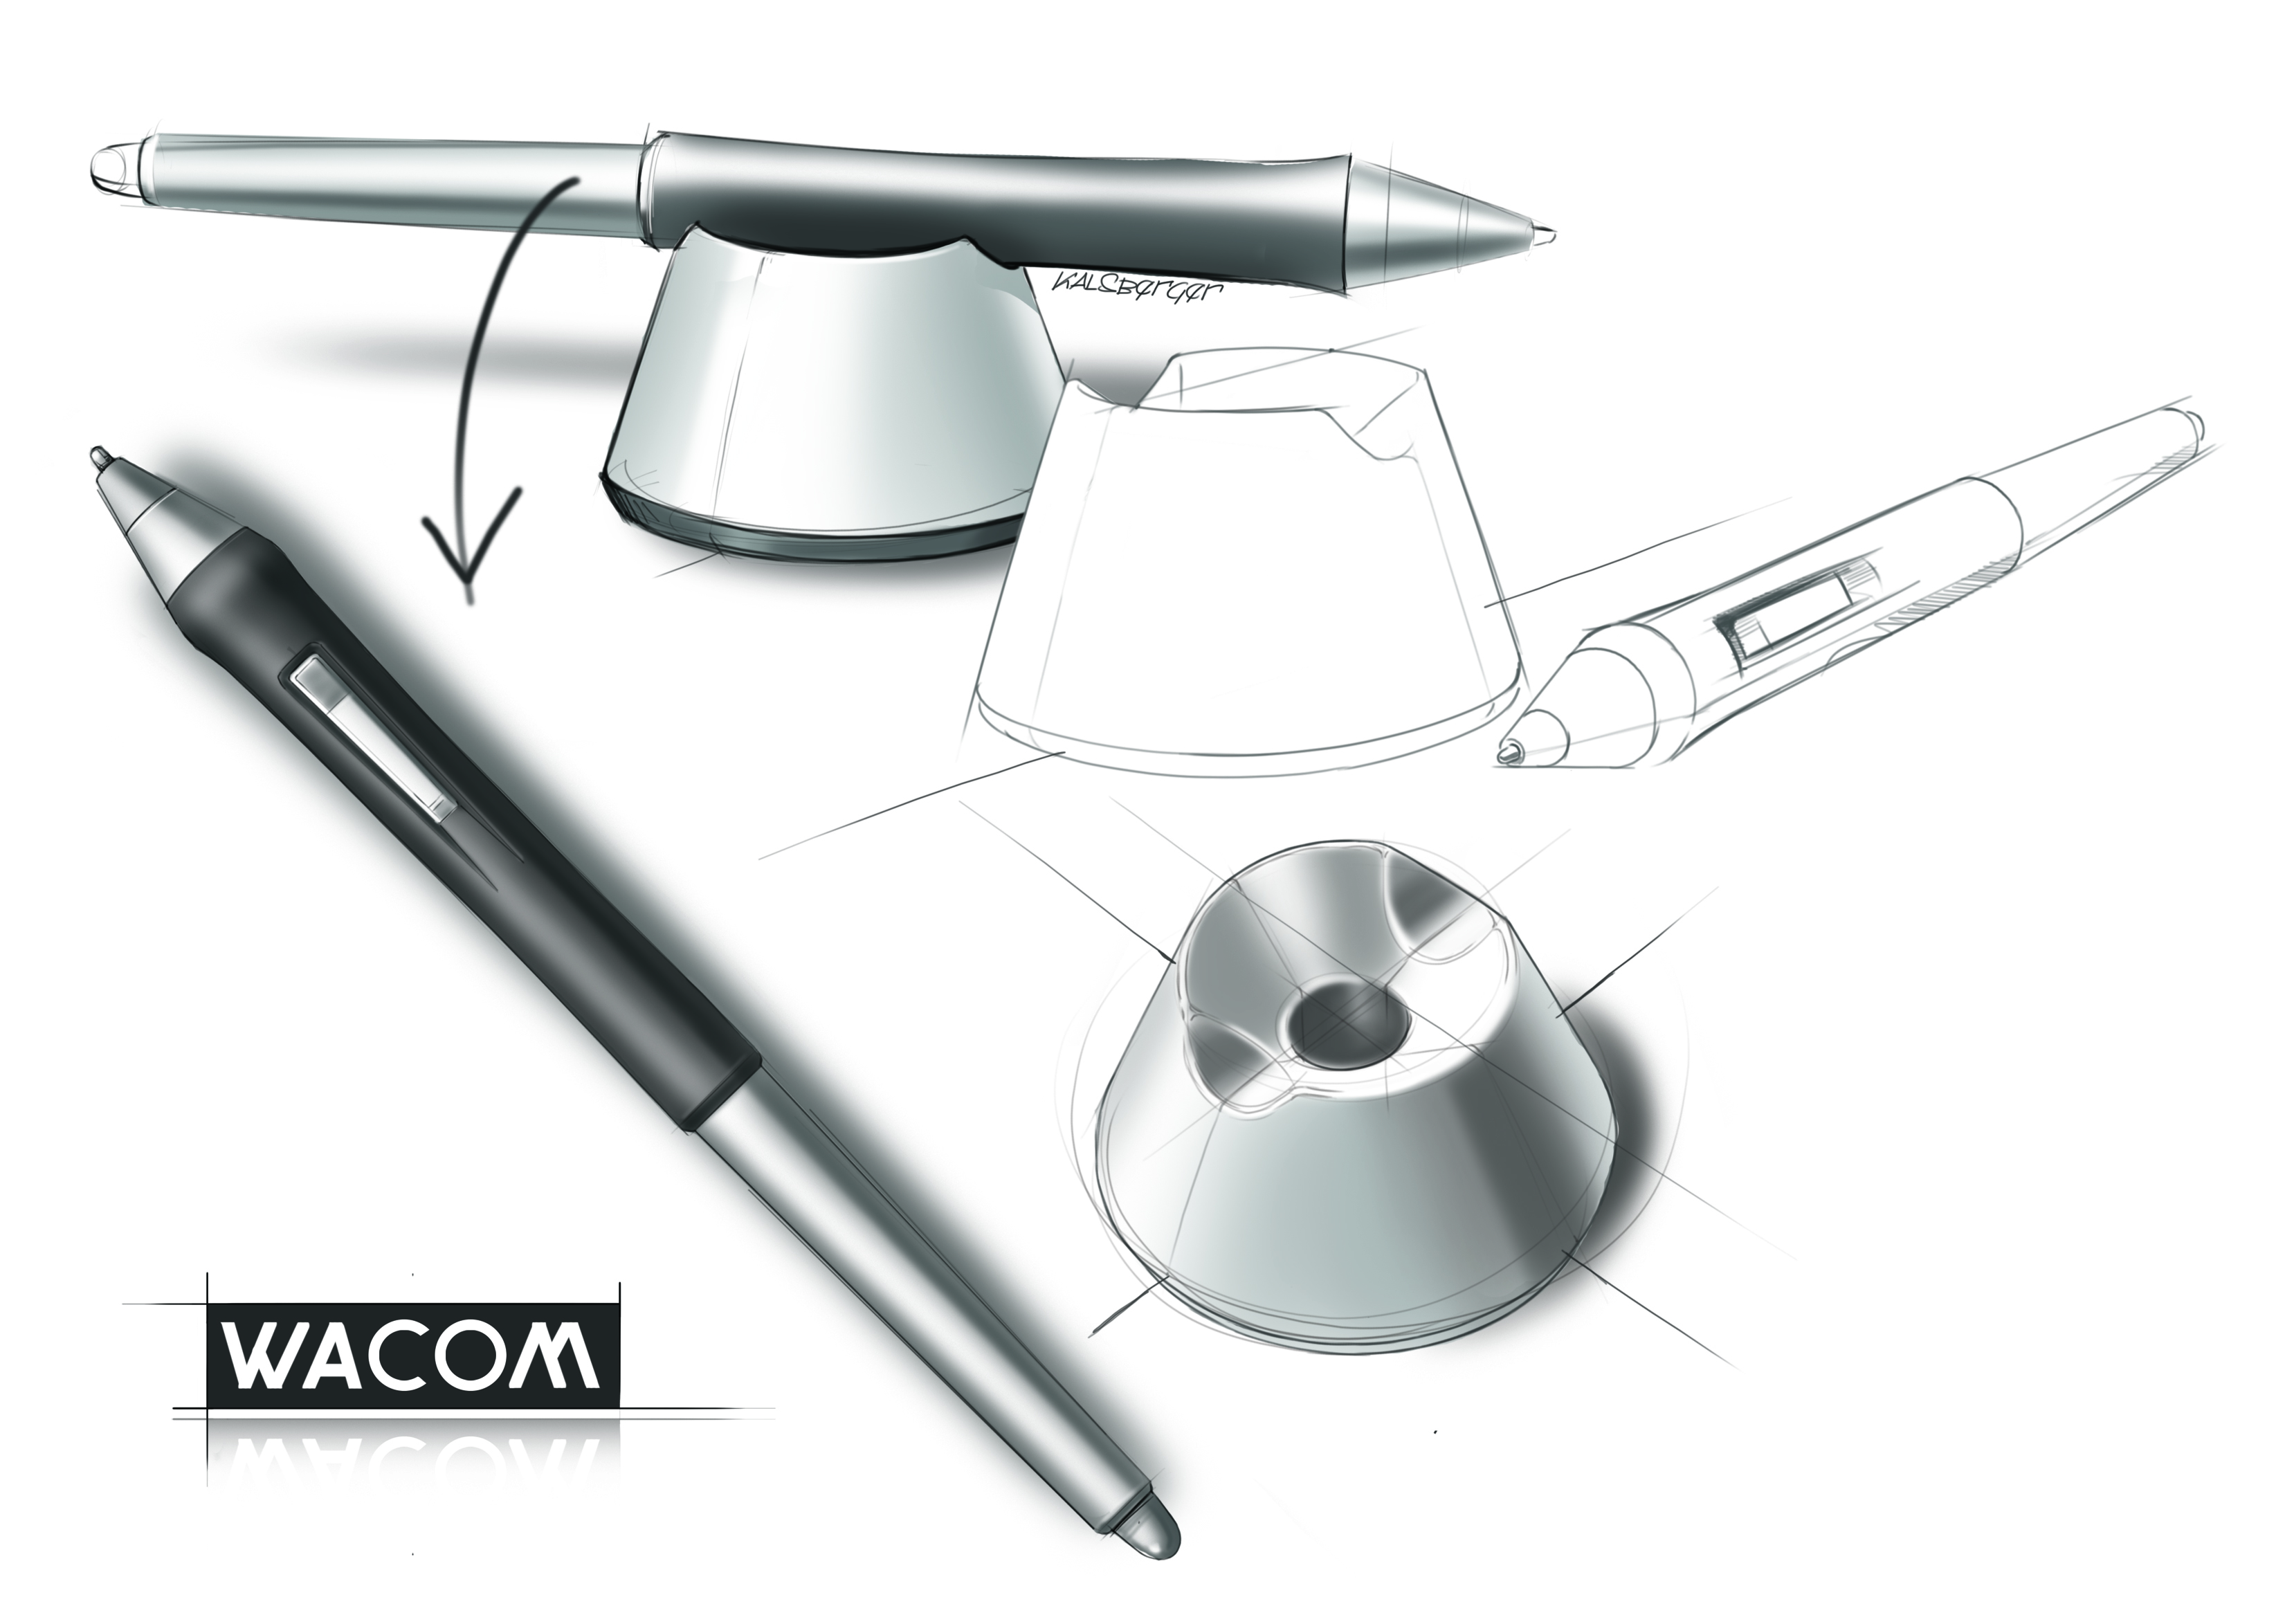
\includegraphics[width=9cm]{gfx/title_picture} \\ \medskip

		\vfill

        \myDegree \\ \medskip   
        %\myDepartment \\                            
        %\myFaculty \\
        %\myUni \\ \bigskip

        \myTime

        \vfill                      

    \end{center}  
  \end{addmargin}       
\end{titlepage}   
\thispagestyle{empty}

\hfill

\vfill

\noindent\myNameA \& \myNameB: \textit{\myTitle,} \myDegree, \textcopyright\ \myTime

%\bigskip
%
%\noindent\spacedlowsmallcaps{Supervisors}: \\
%\myProf \\
%\myOtherProf \\ 
%\mySupervisor
%
%\medskip
%
%\noindent\spacedlowsmallcaps{Location}: \\
%\myLocation
%
%\medskip
%
%\noindent\spacedlowsmallcaps{Time Frame}: \\
%\myTime

%*******************************************************
% Dedication
%*******************************************************
\thispagestyle{empty}
%\phantomsection 
\refstepcounter{dummy}
\pdfbookmark[1]{Widmung}{Widmung}

\vspace*{9cm}

\begin{center}
    %\emph{Coming together is a beginning, 
	%staying together is progress, 
	%and working together is success.} \\ \medskip
	\emph{Zusammenkommen ist ein Beginn,
	Zusammenbleiben ein Fortschritt, 
	Zusammenarbeiten ein Erfolg.} \\ \medskip
    --- Henry Ford    
\end{center}

\medskip

\begin{center}
    An alle Designer. \\ \smallskip
\end{center}
\cleardoublepage%*******************************************************
% Declaration
%*******************************************************
\refstepcounter{dummy}
\pdfbookmark[1]{Erklärung}{Erklärung}
\chapter*{Erkl{\"a}rung zur Verfassung der Arbeit}
\thispagestyle{empty}
% Hiermit erklären wir, dass wir die vorliegende Arbeit selbstständig verfasst und sämtliche in Anspruch genommenen Hilfsmittel und Quellen in der Arbeit als solche gekennzeichnet haben. Die von uns verfassten Kapitel wurden gerecht aufgeteilt und im Inhaltsverzeichnis entsprechend markiert. \\
% Diese Arbeit wurde bisher weder im Inland noch im Ausland in irgendeiner Form als Prüfungsarbeit vorgelegt.
% \bigskip
%  
% \noindent\textit{\myLocation, \myTime}
% 
% \bigskip
% 
% \begin{tabularx}{\textwidth}{p{5cm}X}
% 
% \begin{flushright}
%     \begin{tabular}{m{4.5cm}}
%         \\ \hline
%         \centering\myNameA\\
%     \end{tabular}
% \end{flushright}
% &
% \begin{flushright}
%     \begin{tabular}{m{4.5cm}}
%         \\ \hline
%         \centering\myNameB\\
%     \end{tabular}
% \end{flushright}
% 
% \end{tabularx}


\hspace{0.55cm}\begin{tabularx}{\textwidth}{m{0.47\textwidth}m{0.47\textwidth}}

\noindent\begin{flushleft}
    \myNameA \\
	Kanitzgasse 35/2/4, \\
	1230 Wien
\end{flushleft}
&
\noindent\begin{flushleft}
    \myNameB \\
	Lustkandlgasse 39/30, \\
	1090 Wien
\end{flushleft}

\end{tabularx}

\bigskip

Hiermit erklären wir, dass wir diese Arbeit selbständig verfasst haben, dass wir die verwendeten Quellen und Hilfsmittel vollständig angegeben haben und dass wir die Stellen der Arbeit - einschließlich Tabellen, Karten und Abbildungen -, die anderen Werken oder dem Internet im Wortlaut oder dem Sinn nach entnommen sind, auf jeden Fall unter Angabe der Quelle als Entlehnung kenntlich gemacht haben.

\bigskip

\bigskip

\noindent\begin{tabularx}{\textwidth}{m{0.47\textwidth}m{0.47\textwidth}}

\noindent\begin{flushleft}
    \begin{tabular}{m{4.5cm}}
        \\ \hline
        \centering\myNameA\\
    \end{tabular}
\end{flushleft}
&
\noindent\begin{flushleft}
    \begin{tabular}{m{4.5cm}}
        \\ \hline
        \centering\myNameB\\
    \end{tabular}
\end{flushleft}

\end{tabularx}

\begin{center}
    \begin{tabular}{m{4.5cm}}
        \\ \hline
        \centering(Ort, Datum)\\
    \end{tabular}
\end{center}
\cleardoublepage%*******************************************************
% Abstract
%*******************************************************
%\renewcommand{\abstractname}{Abstract}
\pdfbookmark[1]{Abstract}{Abstract}
\begingroup
\let\clearpage\relax
\let\cleardoublepage\relax
\let\cleardoublepage\relax

\chapter*{Abstract}
When working together on a project, people share their documents, materials and tools. Real life objects allow users to comunicate thoughts, ideas and concepts very easily in short time. There has been some effort to recreate a similar experience when using digital media for collaborative work. Unfortunately, existing solutions still do not offer an efficient and transparent interface between real-life and digital artifacts which is the reason why people still prefer conventional methods for collaboration. \\
The following paper describes possible implementations to use traditional design methods on digital artefacts in theory and in practice. \scribbler is one representative of a collaborative system which uses \emph{sketching}, the most important design method, to find this missing link.

\vfill

\pdfbookmark[1]{Kurzfassung}{Kurzfassung}
\chapter*{Kurzfassung}
Kollaboratives Arbeiten bedeutet das Teilen von Materialien, Dokumenten und Werkzeugen. Herkömmliche, greifbare Medien schaffen eine Kommunikationsebene zwischen den Personen, auf der es möglich ist, Gedanken, Ideen und Konzepte rasch und zugänglich aufzubereiten. In der Vergangenheit sind schon einige Versuche unternommen worden, diese Art des Arbeitens auf digitalen Medien umzusetzen. So gibt es bereits Ansätze, die die Zusammenarbeit auf einem gemeinsamen großen Display ermöglichen sollen. Jedoch stößt man bei der Arbeit mit diesen kollaborativen Systemen immer wieder auf Barrieren, da es bisher noch nicht gelungen ist, eine effiziente und transparente Schnittstelle zwischen analogen und digitalen Objekten zu schaffen.\\
Anhand theoretischer und praktischer Ansätze beschreibt die folgende Arbeit die Unterstützung traditioneller Arbeitsweisen von Designern auf digitalen Objekten. Das kollaborative System \scribbler setzt auf die wohl wichtigste Designmethode, das \emph{Skizzieren}, und versucht eine barrierefreie Schnittstelle zwischen realen und digitalen Objekten zu schaffen.

\endgroup			

\vfill
%\cleardoublepage%*******************************************************
% Publications
%*******************************************************
\pdfbookmark[1]{Publications}{publications}
\chapter*{Publications}
Some ideas and figures have appeared previously in the following publications:

\bigskip

\noindent Put your publications from the thesis here.
\cleardoublepage%*******************************************************
% Acknowledgments
%*******************************************************
\pdfbookmark[1]{Danksagungen}{Danksagungen}

\begin{flushright}{\slshape    
    We have seen that computer programming is an art, \\ 
    because it applies accumulated knowledge to the world, \\ 
    because it requires skill and ingenuity, and especially \\
    because it produces objects of beauty.} \\ \medskip
    --- \defcitealias{knuth:1974}{Donald E. Knuth}\citetalias{knuth:1974} \citep{knuth:1974}
\end{flushright}

\bigskip

\begingroup
\let\clearpage\relax
\let\cleardoublepage\relax
\let\cleardoublepage\relax
\chapter*{Danksagung}
Wir möchten uns an dieser Stelle sehr herzlich bei allen bedanken, die uns bei unserem Projekt, den Auswertungen und dem Schreiben der vorliegenden Arbeit unterstützt haben. 

Besonderer Dank gilt dabei jenen Personen, die sich bereit erklärten \scribbler zu testen. Durch sie fanden wir nicht nur Bestätigung in unserer Arbeit, sondern gewannen auch wichtige Erkenntnisse und Anregungen zur Weiterentwicklung.

Tom und Tom, wir bedanken uns bei euch für eure Unterstützung und Beratung und Peter, vielen vielen Dank für diese tolle Illustration.

Ein großes Dankeschön gebührt auch unserem Betreuer, Ao. Univ.-Prof. Peter Purgathofer für die Inspiration, Motivation und Unterstützung, die er in dieser Zeit für uns gewesen ist.

\medskip \noindent \emph{--- Danke.}

\pagebreak

\chapter*{Thomas}
Mein größter Dank gebührt meiner geliebten Familie, die mir immer Rückenwind gegeben und mich stets motiviert hat. Mum, Dad, Gerry --- ohne euch und eure Unterstützung wäre all dies nicht möglich gewesen. Ihr habt mir immer vertraut und mir Selbstbewusstsein geschenkt. Dafür bin ich euch ewig dankbar.

Anna --- danke, dass du da bist. Danke, dass du mich begleitest. Danke dass du immer Geduld und Verständnis zeigst und danke, dass du diese Zeit so unglaublich schön für mich machst. 

\pagebreak

\chapter*{Clemens}

\endgroup


\hfill

\vfill

\vspace*{0.5cm}

\begin{center}
\begin{footnotesize}
	\textcolor{Gray}{
		\begin{tabular}{rp{7cm}}
			\cs & verfasst von Clemens Sagmeister \\
			\tn & verfasst von Thomas Nägele \\
			\cs \tn & verfasst von Clemens Sagmeister \& Thomas Nägele \\
		\end{tabular} }
\end{footnotesize}
\end{center}



\pagestyle{scrheadings}
\cleardoublepage%*******************************************************
% Table of Contents
%*******************************************************
%\phantomsection
\refstepcounter{dummy}
\pdfbookmark[1]{\contentsname}{tableofcontents}
\setcounter{tocdepth}{2} % <-- 2 includes up to subsections in the ToC
\setcounter{secnumdepth}{3} % <-- 3 numbers up to subsubsections
\manualmark
\markboth{\spacedlowsmallcaps{\contentsname}}{\spacedlowsmallcaps{\contentsname}}
\tableofcontents 
% adding logograms to 1st content page
\addtocontents{toc}{\graffito{\\[0.75cm] \textcolor{Gray}{\protect \cs \protect \tn} \\[6.15cm] \textcolor{Gray}{\protect \cs} \\[6.65cm] \textcolor{Gray}{\protect \tn} \\[5.15cm] \textcolor{Gray}{\protect \cs}} \par}
% adding logograms to 2nd content page
\graffito{\\[-2.3cm] \textcolor{Gray}{\cs \tn} \\[-8.86cm] \textcolor{Gray}{\cs \tn} \\[-4.85cm] \textcolor{Gray}{\tn}}
\automark[section]{chapter}
\renewcommand{\chaptermark}[1]{\markboth{\spacedlowsmallcaps{#1}}{\spacedlowsmallcaps{#1}}}
\renewcommand{\sectionmark}[1]{\markright{\thesection\enspace\spacedlowsmallcaps{#1}}}

\vspace*{1.8cm}

\begin{footnotesize}
	\textcolor{Gray}{
		\begin{tabular}{rp{9cm}}
			\cs & verfasst von Clemens Sagmeister \\
			\tn & verfasst von Thomas Nägele \\
			\cs \tn & verfasst von Clemens Sagmeister \& Thomas Nägele \\
		\end{tabular} }
\end{footnotesize}

%*******************************************************
% List of Figures and of the Tables
%*******************************************************
\clearpage

\begingroup 
    \let\clearpage\relax
    \let\cleardoublepage\relax
    \let\cleardoublepage\relax
    %*******************************************************
    % List of Figures
    %*******************************************************    
    %\phantomsection 
    \refstepcounter{dummy}
    %\addcontentsline{toc}{chapter}{\listfigurename}
    \pdfbookmark[1]{\listfigurename}{lof}
    \listoffigures

    \vspace*{8ex}

    %*******************************************************
    % List of Tables
    %*******************************************************
    %\phantomsection 
    \refstepcounter{dummy}
    %\addcontentsline{toc}{chapter}{\listtablename}
    \pdfbookmark[1]{\listtablename}{lot}
    \listoftables
        
    \vspace*{8ex}
%   \newpage
    
    %*******************************************************
    % List of Listings
    %*******************************************************      
	  %\phantomsection 
    \refstepcounter{dummy}
    %\addcontentsline{toc}{chapter}{\lstlistlistingname}
    \pdfbookmark[1]{\lstlistlistingname}{lol}
    \lstlistoflistings 

    \vspace*{8ex}
       
    %*******************************************************
    % Acronyms
    %*******************************************************
    %\phantomsection 
    \refstepcounter{dummy}
    \pdfbookmark[1]{Akronyme}{acronyms}
    \markboth{\spacedlowsmallcaps{Acronyms}}{\spacedlowsmallcaps{Acronyms}}
    \chapter*{Akronyme}
    \begin{acronym}[UML]
		\acro{CSCW}{Computer Supported Cooperative Work}
        \acro{HCI}{Human-Computer Interaction}
		\acro{PDF}{Portable Document Format}
        \acro{HTML}{Hypertext Markup Language}
		\acro{WIMP}{Window-Icon-Menu-Pointing Device}
		\acro{GUI}{Graphical User Interface}
		\acro{SDG}{Single Display Groupware}
		\acro{USB}{Universal Serial Bus}
		\acro{CAD}{Computer-Aided Design}
    \end{acronym}

	\vspace*{8ex}
       
    %*******************************************************
    % Extracts
    %*******************************************************
    %\phantomsection 
    \refstepcounter{dummy}
    \pdfbookmark[1]{Ausz\"uge}{extracts}
    %\markboth{\spacedlowsmallcaps{Extracts}}{\spacedlowsmallcaps{Extracts}}
    %\chapter*{Extracts}
	\listofextracts
                         
\endgroup

\cleardoublepage
%********************************************************************
% Mainmatter
%*******************************************************
\pagenumbering{arabic}
% use \cleardoublepage here to avoid problems with pdfbookmark
%\cleardoublepage\part{Einleitung}
\cleardoublepage%*******************************************************
% Introduction
%*******************************************************
\cleardoublepage
%\pdfbookmark[-1]{Epilog}{Epilog}
\phantomsection
\addtocontents{toc}{\protect\vspace{\beforebibskip}} % to have the bib a bit from the rest in the toc
\addcontentsline{toc}{chapter}{\tocEntry{Einleitung}}
%\begin{quote}
%	\begin{flushright}{\slshape    
%	    zitat.} \\ \medskip
%	    --- Max Mustermann \citep{xx:xxxx}
%	\end{flushright}
%\end{quote}
%\pagestyle{empty}

\hfill

\vfill

\begingroup
\let\cleardoublepage\relax
\chapter*{Einleitung} \label{app:introduction}
In den letzten Jahrzehnten wurde viel Forschung betrieben, um die Unterstützung kollaborativer Arbeitssituationen durch technologische Mittel voran zu treiben. Vor Allem im Web stieg die Anzahl an Tools zur entfernten Zusammenarbeit an. Gleichzeitig musste man aber feststellen, dass die bequeme Onlinekollaboration auch Nachteile mit sich brachte. Einfache Eigenschaften die bei traditionellen Gruppenarbeiten existieren, wie Augenkontakt, Gestik etc. verschwanden. Aus diesem Grund haben kollaborative Meetings bis dato nicht an Beliebtheit verloren. Besonders Designer verbringen viel Zeit in Meetings um zusammen mit anderen Ideen zu erarbeiten. Ihr wichtigstes Werkzeug dafür sind Stift und Papier, mit dessen Hilfe sie Notizen und einfache Skizzen anfertigen können.\\
Da aber auch hier die Technisierung nicht halt machte und Designer vermehrt mit digitalen Medien zu tun haben, kommt es oft zu ungewolltem Mehraufwand. Designs die nur elektronisch existieren, können zwar meist in einer geeigneten Form (z.B. mittels Projektor) präsentiert werden, jedoch können Anmerkungen, Notizen oder neue Ideen nie direkt auf das digitale Design geschrieben oder gezeichnet werden. \\
Es existieren zwar bereits Systeme, die das kollaborative Skizzieren auf einem gemeinsamen Display ermöglichen, jedoch werden Skizzen an das jeweilige System gebunden, was es unmöglich macht jegliche Inhalte zu bearbeiten.

\medskip Mit der vorliegenden Arbeit, erläutern wir die Problemfelder dieser Situation und zeigen mit dem Projekt \scribbler einen möglichen Lösungsansatz. In den folgenden Kapiteln wollen wir zunächst in \autoref{ch:research} bestehende Systeme beschreiben und im Zuge dessen, wichtige Anforderungen an ein solches System sammeln. \autoref{ch:designTheorie} und \autoref{ch:kollaborativesDesign} erklären Arbeitsweisen von Designteams mittels Methoden und Verhaltensweisen in kollaborativen Settings. In \autoref{ch:DesignVSComputer} spezifizieren wir den Unterschied zwischen dem Arbeiten mit traditionellen und digitalen Medien. Anschließend charakterisieren wir in \autoref{ch:CSCWDesign} gruppenbasierte Systeme, bevor wir in \autoref{ch:scribbler} alle gewonnen Erkenntnisse mit Hilfe unseres Prototypen veranschaulichen wollen.

\bigskip \emph{Anmerkung: Über \graffito{\(\clubsuit\)}die gesamte Arbeit werden Anmerkungen, seitlich durch das \begin{footnotesize}\(\clubsuit\)\end{footnotesize}-Symbol gekennzeichnet. Kommentare \graffito{Kommentar}werden ebenfalls seitlich platziert.}
\endgroup




\cleardoublepage\part{Theorie}
%*****************************************
\chapter{Research Field}\label{ch:research}
%*****************************************
In der Arbeitswelt kommt es immer wieder zu Situationen, in der sich mehrere Personen treffen um zusammen Probleme zu diskutieren. Statistiken besagen, dass Büroangestellte sogar bis zu 70 Prozent ihrer Arbeitszeit in Meetings verbringen \cite{panko:1993}. Die meisten Meetings werden mit Hilfsmittel wie Whiteboards, Flipcharts oder Notizblöcke abgehalten, da meistens Notierungsbedarf bei neuen Ideen, Problemlösungen etc. besteht. Computer können dabei sehr hilfreich sein, wäre da nicht die Hürde der Dateneingabe die zu bewältigen ist. Herkömmliche Eingaben via Maus und Tastatur verlangsamen den natürlichen explorativen Charakter eines Meetings. Elektronische Skizzierwerkzeuge inklusive gemeinsam verwendbarer Zeichenoberflächen können hier Abhilfe für kollaboratives Arbeiten schaffen. 

\medskip Das folgende Kapitel soll anhand von Beispielen und Projekten aus der Literatur zeigen, durch welche Methoden Meetings bzw. im speziellen Designsessions unterstützt werden können. Besonderer Augenmerk soll dabei auf das Skizzieren als Designmethode und kooperatives Arbeiten in CSCW\footnote{Computer Supported Cooperative Work} Umgebungen liegen.

\section{Arbeitsweisen von Designteams}
Um herauszufinden mit welchen Methoden oder Werkzeugen man kollaborative Meetings und im Zuge dessen den Designprozess unterstützen kann, muss man zuerst wissen wie Designer zusammen arbeiten. John Tang und Larry Leifer versuchten in \cite{Tang:1988p279} als Teil einer Studie, mittels empirischen Daten das Verhalten von Designern in Meetings zu untersuchen. Dazu bildeten sie ein Framework und konzentrierten sich auf deren Arbeitsaktivitäten wie \emph{Auflisten}, \emph{Zeichnen} und \emph{Gestikulieren}, welche sie den zugehörigen Kontext zuordneten. Um diesen einzuschränken, bildeten sie vier Funktionen, die den Hauptzweck der Aktivitäten beschreiben: \emph{Festhalten von Informationen}, \emph{Vermitteln von Ideen}, \emph{Darstellen von Ideen} und \emph{Erlangen von Aufmerksamkeit}. In einem Framework (siehe \autoref{fig:Abbildung1}) stellten sie diese gegenüber und verwendeten die Daten zur Auswertung.

\medskip Obwohl sich Tang und Leifer mit ihrer Arbeit gezielt auf den Designprozess zubewegen, erwarten sie dadurch auch relevante Ergebnisse für kollaboratives Arbeiten im Allgemeinen. \par Kollaboratives Arbeiten ist für Designer eine gängige Art Probleme anzugehen und kann von den sonstigen individuellen Aktivitäten deutlich abgegrenzt werden, wie auch frühere empirische Designstudien bestätigen können (\cite{Ullman:1987}, \cite{Ballay:1987}, \cite{Akin:1978}, \cite{Lera:1983}).
In ihrer Studie führten sie 8 Sessions mit Teams zu je 3-4 Personen durch, welche jeweils eineinhalb Stunden dauerten. Die Gruppen trafen sich dafür in Konferenzräumen und saßen um einen Tisch mit einem großen Bogen Papier als Schreibunterlage. Jede Gruppe arbeitete zwar an einer anderen Designaufgabe, jedoch waren alle Teil des Designs eines Mensch-Maschinen Interfaces für ein >>smartes<< (Mikroprozessor gesteuertes) Gerät.
Die Analyse der Tests wurde durch das NoteCards Hypertext Environment \cite{Halasz:1986:NN:29933.30859} erheblich vereinfacht. Das System half die Daten zu strukturieren und aufzubereiten. \autoref{fig:Abbildung2} zeigt einen Auszug des Transkripts der ersten Session mit Anmerkungen zu einzelnen Aktivitäten und einen Teil der Schreibunterlage, welche die dazu erstellte Skizze beinhaltet. Jede Aktivität wurde anhand der Funktionen des Frameworks kategorisiert und abgezählt, um in Folge dessen die Daten statistisch auszuwerten. \autoref{fig:Abbildung3} veranschaulicht die Ergebnisse.

\medskip Wie die Abbildung zeigt, sind knapp die Hälfte (46\%) aller Aktivitäten von illustrativen Charakter, was die Wichtigkeit von Skizzen belegt. Zusätzlich kommt der Vermittlung und Darstellung von Ideen (zusammen 43\%) auch große Bedeutung zu.
Anmerkung: An diesem Punkt der Arbeit soll noch nicht auf die gesamten Erkenntnisse der Analyse eingegangen werden, sondern lediglich auf die der Ideenentwicklung. Die weiteren Ergebnisse werden in den Kapitel Single VS Group Design und CSCW \& Design behandelt.

\medskip Die Schreibunterlage spielt im Prozess der Ideenentwicklung, neben der des Festhaltens von Informationen und der Vermittlung von Ideen, eine aktive Rolle. Die Unterstützung dieses Prozesses (zb. durch elektronische Hilfsmittel) ist aber alles andere als unproblematisch, wie beispielsweise die Frustrationen von Designer beweisen, die versuchen konventionelle CAD Tools für die Weiterentwicklung von Ideen - von konzeptionellen Skizzen zu formellen Spezifikationen - zu verwenden. Dieser Aspekt zeigt die Verwendung der Schreibunterlage als Teil eines interaktiven Prozesses, anstatt der Reduzierung dessen auf ein Text-Grafik Artefakt. 
Die Studie beobachtete 2 Schlüsselmerkmale, auf die Designer bei der Entwicklung von Ideen zurückgriffen: a) In der Lage sein ohne Weiteres Darstellungen von Ideen auf einer Schreibunterlage auszuprobieren, und b) diese Darstellungen stufenweise in genaue Artefakte weiterzuverarbeiten - oft durch die Zusammenarbeit mit anderen Partizipienten. \cite{Tang:1988p279}

%\clearpage
\begin{figure}
        {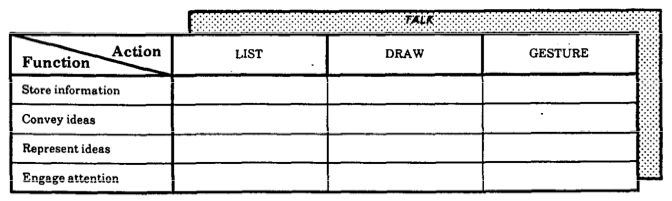
\includegraphics[width=1\linewidth]{gfx/Abb1}}
		\caption[Framework zur Untersuchung von Designaktivitäten.]{Das Framework zur Untersuchung von Designaktivitäten. In ihm werden die Aktivitäten den zweckmäßigen Funktionen gegenübergestellt. Es dient als empirische Grundlage. }\label{fig:Abbildung1}
\end{figure} 

\begin{figure}[bth]
        \myfloatalign
        \subfloat[Transkriptauszug]
        {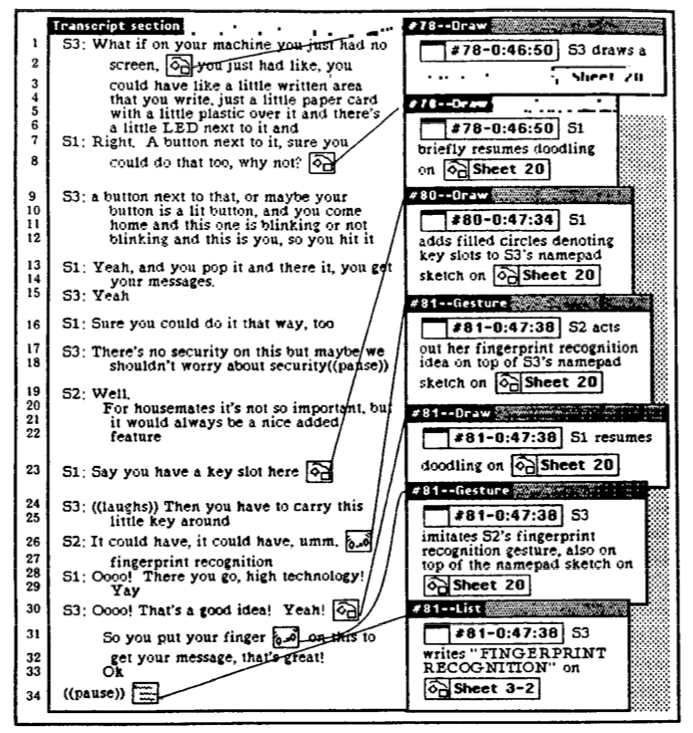
\includegraphics[width=.65\linewidth]{gfx/Abb2_1}} \quad
        \subfloat[Artefakt]
        {\label{fig:Abbildung2b}%
         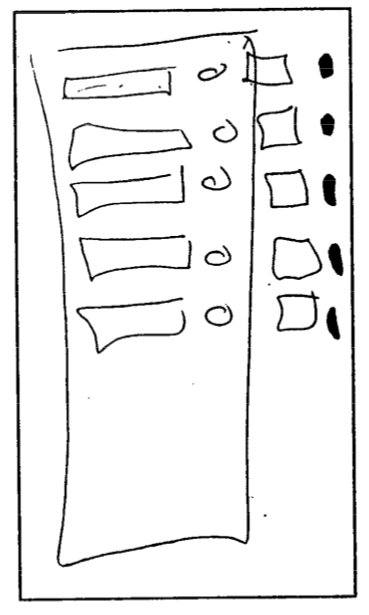
\includegraphics[width=.25\linewidth]{gfx/Abb2_2}} \\
        \caption[Auszug des Transkripts inklusive dazugehöriges angefertigtes Artefakt der ersten Designsession.]{Ein Auszug des Transkripts, erstellt mit Hilfe von NoteCards \cite{Halasz:1986:NN:29933.30859}, inklusive dazugehörigen  Artefakt der ersten Designsession. Es zeigt wie jeder Teilnehmer in kürzester Zeit einen eigenen Gedanken äußert und diesen im Artefakt manifestiert.}\label{fig:Abbildung2}
\end{figure}

\begin{figure}
        {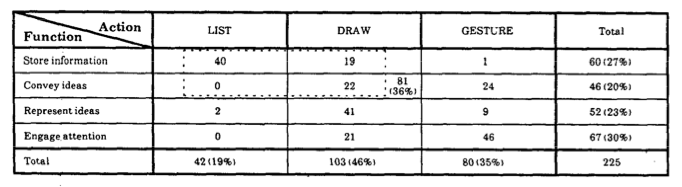
\includegraphics[width=1\linewidth]{gfx/Abb3}}
		\caption[Statistische Ergebnisse der ersten Designsession.]{Statistische Ergebnisse der ersten Designsession. Alle Aktivitäten wurden dafür im Framework anhand der Funktionen kategorisiert und anschließend abgezählt.}\label{fig:Abbildung3}
\end{figure}
\clearpage

\medskip Gemeinsam verwendbare Zeichenoberflächen spielen auch laut Sara Bly \cite{Bly:1988:UDS:62266.62286} eine besonders wichtige Rolle in Designsessions mit mehreren Teilnehmern. 
Bly beobachtete das Skizzierverhalten zweier Personen in Face-to-Face Designsessions und zeichnete diese für spätere Anaylsen auf Video auf. Bei der Auswertung stellte sie fest, dass nahezu die Hälfte aller Aktivitäten, in denen Gebrauch von Schreibwerkzeugen gemacht wurde, Skizzen waren. Noch interessanter war aber die Tatsache, dass sich im Laufe der Session verschiedene Zeichenbereiche herauskristallisiert haben. So entstanden einzelne Bereiche in denen nur ein Designer gezeichnet hat und Bereiche die zusammen benutzt wurden. 78\% aller Aktivitäten fanden jedoch im gemeinsamen Bereich statt und 25\% aller Aktivitäten eines Designers entstanden im Anschluss zu einer Zeichnung eines anderen Designers. Die Analyse zeigt also die Wichtigkeit von gemeinsamen Bereichen in Designsessions mit mehreren Teilnehmern. Zusätzlich spielten Gesten und Betonungen in Erläuterungen eine wichtige Rolle, welche die Notwendigkeit der physischen Anwesenheit nahelegt.

\section{Skizziertools in kooperativen Settings}
Dies als Ansporn und Grundlage für weitere Arbeiten nahm sich das Department of Computer Science auf der Universität in Toronto und entwickelte XSketch: ein Multiuser Skizzierwerkzeug für X11\footnote{X11 ist ein Softwaresystem für UNIX Plattformen, dass ein Grafisches User Interface (GUI) zur Verfügung stellt - auch bekannt als X-Windows.}, dass Jefferey J. Lee bereits 1990 in \cite{Lee:1990:XMS:91478.91510} vorstellt und dessen Eigenschaften ich folgend kurz beschreiben will.
Die Grundidee von XSketch ist ein simples Werkzeug für Multiuser Design- und Brainstormingsessions bereitzustellen. Da es aber auch für einzelne Benutzer geeignet sein soll, hat der Multiuserfaktor nur wenig Einfluss auf das User Interface. Es setzt auf eine Server-Client Architektur, in der alle Nachrichten und Entscheidungen zentral gesteuert werden und Benutzer via TCP/IP Protokoll kommunizieren. Das Zeichenmodell kann man mit einem Notizblock oder Flipchart vergleichen, in dem Benutzer auf leeren Seiten zeichnen und zwischen mehreren Seiten hin und her >>blättern<< können. Zeichnungen basieren auf ein objektorientierten Ansatz, sodass man leicht ganze Objekte ausschneiden und kopieren kann. Den Benutzern stehen Polylinien\footnote{Polylinien sind eine Aneinanderreihung von Linien. In der Computergrafik werden sie zur Annäherung an Kurven benutzt.}, Rechtecke und simpler Text als Objekte zur Verfügung. Die Interaktion basiert dabei hauptsächlich auf Mauseingaben, die Tastatur wird lediglich zur Eingabe und Änderung von Texten und Dateinamen verwendet. Die meisten Editieroperationen sind ebenfalls an die Mausbuttons gebunden. 
Mit dem Vorsatz das Interface so schlicht wie möglich zu halten, existieren relativ wenig Modi und keine Möglichkeit Attribute wie Linienart, -stärke, Pfeilspitzen etc. zu ändern. Dafür ist es möglich einen Telepointer durch Druck auf eine bestimmte Maustaste einzublenden, um so das Gezeichnete für die anderen Benutzer hervorheben zu können. Diese Funktion soll als Ersatz für Gesten dienen.
Die einzige Multiuser-Funktion ist der >>Invite Button<<, der dazu benutzt werden kann um anderen Benutzern Nachrichten zu schicken und sie zu einer Session einzuladen. Nehmen diese teil, können sie alle Objekte ändern, nicht nur die eigenen. Ansonsten unterscheidet sich eine Multi-User Session kaum von einer Single-User Session.

\medskip Obwohl der Prototyp von XSketch allen anfänglichen Zielen und Anforderungen der Projektgruppe entspricht, gibt es nach Lees Erfahrungen in einigen Fällen Verbesserungspotential. So wirkt z.B. das Zeichnen von Skizzen unbefriedigend. Ein möglicher Lösungsansatz für dieses Problem wäre, neue grafische Objekte wie Ellipsen oder Splines zur Objektauswahl hinzuzufügen und das Einfügen von Bitmapbildern zu erlauben, um so das Repertoire an Tools aufzustocken. \graffito{Ein gutes Multi- User Skizzier Programm benötigt eine große Auswahl an Tools oder sollte sich durch und durch auf Freihandzeichnungen beschränken.} Im Gegensatz dazu könnte man das Repertoire aber auch verringern und durch und durch auf reine Freihandzeichnungen setzen. Welcher der bessere Ansatz wäre, müsse ausprobiert werden.
Ein weiterer verbesserungsbedürftiger Punkt ist das strikte Cut\&Paste Modell. Eigentlich anfangs bewusst dafür entschieden um Kollisionen im Datenmanagement vorzubeugen, steht das Entwicklungsteam dadurch vor Usabilityproblemen. Durch die Tatsache, dass man existierende Objekte nicht nachträglich ändern kann, entsteht Frust bei den Benutzern. Ein optimistisches Sperrmodell\footnote{Sperrmodelle in der elektronischen Datenverarbeitung sind Mechanismen die Datenbankressourcen sperren, um zu verhindern, dass mehrere Datenzugriffe gleichzeitig stattfinden können. Man unterscheidet zwischen optimistischen und pessimistischen Sperrstrategien. Eine pessimistische Sperrstrategie schützt die Integrität der Datenbank, indem Datenbankressourcen während der gesamten Dauer einer Transaktion von Anfang bis Ende gesperrt werden. Eine optimistische Sperrstrategie hingegen senkt die Isolationsstufe, so dass weniger Sperren auf die Datenbankressourcen angewandt werden. Auf diese Weise können mehr Anwendungen gleichzeitig auf eine Datenbank zugreifen, was den Durchsatz potenziell erhöhen kann.} könnte, im Gegensatz zu konventionellen zentralisierten (pessimistischen) Sperrmodellen, das Selektieren und nachträgliche Ändern von Objekten ohne lästige Verzögerung ermöglichen. \graffito{Nachträgliches Ändern von Skizzen und eine dazugehörige Undo- Funktion sind wünschenswert.}Erstrebenswert wäre diesbezüglich auch eine dazugehörige Undo Funktion, welche die derzeitige Pseudo-Undo Funktion mittels Löschen ersetzt.
Wie auch schon Bly feststellte, ist in einer Designsession mit mehreren Teilnehmern der Prozess des Zeichnens für den Designprozess genau so wichtig wie die Zeichnungen selbst. \cite{Bly:1988:UDS:62266.62286} Aus diesem Grund ist es wichtig, dass alle Teilnehmer sehen können was die anderen machen. \graffito{Alle Teilnehmer müssen stets über die Tätigkeiten der anderen im Bilde sein.}Leider können Benutzer von XSketch nicht sehen, wenn andere Benutzer Objekte erstellen oder selektieren, da der Vorgang bis zu seinem Abschluss rein lokal abläuft. Diese Entscheidung ist laut Lee schlichtweg ein Fehler und muss unbedingt ausgebessert werden. Ebenso das Ausbleiben einer Möglichkeit um untereinander kommunizieren zu können, sieht er als Fehlgriff, da es im geplanten Setting oft vorkommt dass viele User in einem großen Raum verteilt sitzen und kein Telefon bei sich haben um erreichbar zu sein. Hier wäre eine integrierte Nachrichtenfunktion im Programm denkbar, wie z.B. auch in MUSK \cite{Crampton:1987} umgesetzt wurde. Das würde den Benutzern zusätzlich helfen eine Übersicht über alle Teilnehmer zu bekommen. 
Schließlich, resümiert Lee, war es rückblickend auch falsch anzunehmen, dass sich die Anforderungen von Multi-User Systemen von Single-User Systemen nicht unterscheiden. Der Prototyp wurde in simplen Designsessions mit einem, zwei und drei Benutzer(n) getestet und zeigte zwar über eine 19,2Kbaud Verbindung eine gute Performance, jedoch beschränken die oben genannten \graffito{Ein Grafiktablet in Verbindung mit einem Flatscreen wäre ein ideales Setting für ein Multi- User Skizziertool.}Probleme den Einsatz noch auf Institutsexperimente.
Unglücklicherweise zeigten die Tests auch, dass ein Maus basierendes System für interaktive Skizziersessions nicht ideal ist. Ein ideales Interface für diese Art von Programm wäre laut Lee ein gut integriertes Grafiktablet in Verbindung mit einem Flatscreen. Das wäre die bestmögliche Annäherung zu einer Technologie, die Stift und Papier ersetzen könne.

\section{Communication and Information Retrieval with a Pen-based Meeting Support Tool}
Das Paper befasst sich mit dem prototypisch implementierten Meeting Support Tool >>We-Met<<. Dieses verwendet ein stiftbasiertes Interface, das durch digitales Skizzieren der Benutzer die Kommunikation während Meetings fördern und die nachträgliche Auswertung der angefertigten Zeichnungen erleichtern soll.

\subsection{We-Met}
We-Met \cite{Wolf:1997p75} kann bei face-to-face Meetings als auch bei geographisch entfernten Meetings zusammen mit einer Telefonkonferenz eingesetzt werden. Jeder Teilnehmer benötigt einen Computer mit einem Bildschirm und einem stiftbasierten Eingabetablett. Die Geräte werden über ein lokales LAN Netzwerk verbunden. Das Interface bietet mehrere gemeinsame Bereiche für Skizzen und Zeichnungen, die nach jedem vollendeten Strich eines Benutzers aktualisiert werden. Somit sehen alle Teilnehmer die Zeichnungen der anderen nahezu in Echtzeit.

Alle Meetings werden aufgezeichnet und können während dessen oder nach Abschluss der Sitzung aufgearbeitet werden. Jeder Zeichenstrich wird mit einem Zeitstempel versehen, sodass der Zeichenprozess Schritt für Schritt vor- und zurückgespult werden kann. Außerdem erlaubt We-Met bestimmte zeitliche und räumliche Zustände der Skizzen mit Tags zu versehen, sodass sie leichter zwischen diesen hin und her springen können. Die Form der Tags ist an Markierungen angelehnt, die Personen auch in ihren echten Notizbüchern verwenden, denn sie können nicht nur aus Textelementen, sondern auch aus handgezeichneten Schnörkeln, Kügelchen oder Sternchen bestehen, wodurch das Anlegen von Tags einfacher und intuitiver wird.

\subsection{Studie: We-Met als Tool zur Kommunikation in Gruppen}
Schon während der Entwicklung von Prototypen ist es wichtig, das Konzept so früh wie möglich zu testen und evaluieren. We-Met wurde daher schon sehr bald in einer Studie mit potentiellen Nutzern getestet. Die Entwickler zogen drei Gruppen mit je drei Teilnehmern und eine Gruppe mit zwei Teilnehmern heran. Die Testpersonen erhielten die Aufgabe unter Gebrauch von We-Met einen Haushaltsroboter zu konzipieren, der Müll aufsammelt und in einen dafür vorgesehenen Behälter wirft. Viel mehr als ein finales Design zu schaffen, ging es darum, möglichst viele Ideen zu generieren und zu skizzieren.

\subsubsection{Resultate}
\begin{itemize}
	\item \textit{Einfacher Zugang durch stiftbasiertes Interface}\\
	Alle Teilnehmer empfanden das stiftbasierte Interface einfach zu benutzen. Es fiel ihnen nicht schwer, während dem Schreiben und Kritzeln der Diskussion zuzuhören und sich aktiv daran zu beteiligen. Das Arbeiten mit einer Tastatur hingegen erfordert bei vielen Personen einen zu hohen kognitiven Aufwand, um einer Diskussion noch mit ausreichender Aufmerksamkeit beiwohnen zu können. Aufgrund dieser Tatsache hat das stiftbasierte Interface das Potenzial, die Produktivität eines solchen Meetings zu erhöhen, denn es erlaubt den Teilnehmern die parallele Durchführung mehrerer Aktivitäten.
	
	Die Testpersonen sprachen, zeichneten, schrieben, gestikulierten eifrig und hielten viel Augenkontakt während der Diskussion, ähnlich wie in herkömmlichen Meetings ohne Unterstützung von Computern. Das stiftbasierte Interface ermöglichte dabei sehr rasche und flüssige Übergänge beim Wechsel zwischen diesen Kommunikationskanälen.
	
	\item \textit{Formen der Interaktion}\\
	Eine der Testgruppen arbeitete in einer höchst kollaborativen Art und Weise zusammen. Häufig definierte eine Person Anforderungen an den Haushaltsroboter und hielt diese handschriftlich fest, während eine andere Person die Anforderungen verfeinerte und Skizzen dazu anfertigte. Interessanterweise wählten diese Form der Interaktion genau jene Teilnehmer, die sich vorher nicht bekannt waren. Alle Gruppen befanden einstimmig, dass es einfacher sei sich in die Diskussion einzubringen, als bei herkömmlichen Meetings in denen Whiteboards eingesetzt werden. Oft bedeutet in jenen Sitzungen etwas beizutragen aufzustehen, zur Tafel zu gehen, und jemand anderem den Stift zu nehmen. Die natürliche Hemmschwelle, die dadurch entsteht, entfällt bei We-Met, da jeder über einen Computer und Eingabestift verfügt. Der kreative Prozess der Ideenfindung kann so optimiert werden.
	
	Die zweite Gruppe an Testpersonen wählte eine andere Form der Interaktion. Nach einer anfänglichen gemeinsamen Diskussion, zeichnete und skizzierte jeder Teilnehmer für sich. Nachdem alle fertig waren, wurden die Ergebnisse hergezeigt und wiederum diskutiert. Die Personen arbeiteten also getrennt parallel. Im weiteren Verlauf der Sitzung kam es auch vor, dass zwei Teilnehmer miteinander diskutierten, während ein Dritter für sich skizzierte. Nachdem die anderen fertig diskutiert hatten, brachte der Dritte seine neuen Ideen ein und zeigte den anderen die angefertigten Skizzen. Durch diese Art der getrennten Parallelität, die We-Met ermöglicht, können potenziell mehr Ideen gefunden werden und das Ergebnis des Meetings somit verbessert werden.
	
	Anders als bei den vorhergehenden, ergab sich in der dritten Testgruppe eine moderierte Form der Diskussion. In den ersten fünfzehn Minuten sprachen alle drei Teilnehmer miteinander, aber nur einer schrieb Notizen mit. Diese Person kontrollierte auch die Diskussion. Man kann hier das typische Modell eines Meetings mit Whiteboard erkennen.
	
	\item\textit{Gemeinsames Produkt}\\
	Auf die Frage >>Was gefällt Ihnen an We-Met?<<, antworteten Teilnehmer aus allen drei Gruppen, sie würden es gut finden, dass es die Möglichkeit biete, ein gemeinsames Produkt hervorzubringen. Im Vergleich zu herkömmlichen Meetings gäbe es ein besseres Allgemeinverständnis in der Gruppe, wodurch Missverständnisse reduziert würden.
	
	\item\textit{Aufteilung der Arbeitsfläche}
	Der getestete Prototyp von We-Met bot den Teilnehmern keinen privaten Platz für Skizzen und Zeichnungen. Einige der Testpersonen wünschten sich eine private Arbeitsfläche zur Aufzeichnung diverser Notizen. Sie wollten Skizzen auch zuerst fertigstellen, bevor sie bereit waren, sie den anderen Teilnehmern zu zeigen. Daher kam es vor, dass manche sich fernab vom eigentlichen Geschehen auf dem Canvas einen eigenen Platz für ihre Zeichnungen suchten. Andere Gruppen teilten die Arbeitsfläche auf die Teilnehmer auf, sodass jeder seinen eigenen Platz zum Skizzieren fand. Das Fehlen der privaten Arbeitsfläche könnte dazu führen, dass Ideen nicht mitgeteilt werden, da man sie bereits unfertig herzeigen müsste und ebenso könnten Ideen verloren gehen, die man sich für später notiert hätte.
	
	\item\textit{Koordination zwischen den Teilnehmern}
	In keinen der Testgruppen gab es Probleme bei der Koordination und es kam nie vor, dass Teilnehmer aus Versehen versuchten auf dem selben Bereich der Arbeitsfläche zu zeichnen und sich dadurch in die Quere gekommen wären. Da jeder die Zeichenschritte der anderen Teilnehmer Strich für Strich verfolgen konnte, war jedem immer bewusst wer gerade was zeichnete. Schwierigkeiten der Koordination gab es nur bei zwei Aktionen: wechseln der Szene und scrollen der Arbeitsfläche.
	
	Um zu einer neuen Szene zu wechseln, drückt einer der Teilnehmer auf den >>Neu<< Button, wodurch die neue Szene allen Teilnehmern angezeigt wird. Zum Wechseln zu einer bereits vorhandenen Szene, drückt man auf den >>Szenen<< Button und wählt die gewünschte Szene aus der Liste aller zuvor angelegten Szenen aus. Die Liste der Szenen wird nur der Person angezeigt, die auch den >>Szenen<< Button gedrückt hat.
	
	Es gibt drei Aspekte dieses Szenarios, die das Potenzial haben, die Teilnehmer zu verwirren: das Entscheiden, ob die Szene gewechselt werden soll, das Wechseln der Szene und das Erkennen, dass die Szene soeben gewechselt wurde. Die Entscheidung zum Wechsel wurde erwartungsgemäß meist problemlos durchgeführt: Eine Person teilte den anderen Teilnehmern ihre Intention zum Wechsel mit und wartete auf die Zustimmung der anderen.
	
	Die zweite Aktion, das tatsächliche Wechseln der Szene, führte gelegentlich zu Konfusion. Es kam vor, dass nach dem Einverständnis, die Szene zu wechseln, zwei Benutzer gleichzeitig eine neue Szene anlegten, ohne die Aktion des anderen dabei zu bemerken. Dadurch wurde eine Szene mehr angelegt, als die Gruppe im Sinn hatte. Folglich geschah es, dass die Teilnehmer verwirrt waren, als sie zu einem späteren Zeitpunkt versuchten, zur entsprechenden Szene zurück zu wechseln. In einem konkreten Fall wechselte einer der Teilnehmer fünf mal die Szene, beim Versuch, die gewünschte zu finden. Daraufhin versuchte ein anderer Benutzer, die korrekte Szene zu finden und die damit zusammenhängenden Wechsel führten zu leichtem Frust bei einem dritten Teilnehmer.
	
	Gelegentlich realisierten Benutzer nicht, dass eine Szene gewechselt wurde. Das We-Met Konzept sieht zwar vor, für jede Szene einen eindeutigen Namen, bzw. eine eindeutige ID anzuzeigen, aber der Prototyp war zum Testzeitpunkt noch nicht so weit entwickelt, weshalb den Personen weniger Informationen als notwendig angezeigt wurden und Fehlerquellen offen blieben.
	
	Einigen Teilnehmern war nicht ganz klar, dass das Scrolling sich nur auf den eigenen Viewport und nicht den der anderen bezieht. Sie erwarteten sich ein ähnliches Verhalten wie beim Szenenwechsel, welcher von einem Teilnehmer für die gesamte Gruppe durchgeführt wurde. Deshalb gab es oft Probleme die Bereiche zu finden, in denen gerade ein anderer Benutzer zeichnete. Den Testpersonen war es auch nicht einfach möglich, auf den Bildschirm eines anderen zu schauen, um sich bei der Suche nach dem gewünschten Bereich zu behelfen. Die Gruppe versuchte zwar, sich gegenseitig weiterzuhelfen, hatte jedoch Schwierigkeiten dabei. Das Konzept des Scrollens bereitet oft schon Probleme, wenn es um single-user Software geht, und im multi-user Softwarebereich scheint sich diese Problematik noch zu verschärfen.
	
	Diese verlorene Zeit beim Koordinieren der Gruppe ist definitiv ein Rückschritt im Ideenfindungsprozess, aber die gesteigerte Effizienz im kreativen Teil der Arbeit ist ein Schritt in die richtige Richtung.
\end{itemize}

\subsubsection{Zusammenfassung}
Die Studie, durchgeführt mit dem Prototypen des We-Met stiftbasierten Interfacekonzepts, zeigt deutliche Verbesserungen im Kommunikationsprozess während der kreativen Phase der Ideenfindung. We-Met erlaubt verschiedene Formen der Interaktion und ist dadurch sehr flexibel. Neben diesen Vorteilen sind auch sehr konkrete Schwachpunkte des Systems zum Vorschein gekommen. Ein unendlich großer Arbeitsbereich, der auf LCD Monitoren nur stark eingeschränkt dargestellt werden kann, und die Tatsache, dass jeder Benutzer unabhängig scrollen kann, bringt einige Schwierigkeiten in der Gruppenkoordination mit sich.


\section{Team Storm}
Team Storm \cite{Hailpern:2007p113} ist ein groupware System, das die Möglichkeit bietet, parallel an mehreren Ideen zu arbeiten. Es kommt bei Meetings in frühen Konzeptionsphasen zum Einsatz und fördert Kreativität innerhalb der Gruppe. Es konzentriert sich auf das Skizzieren von Ideen und bietet private und gemeinsame Arbeitsflächen, auf denen die Designer arbeiten können.

Das System besteht aus drei Hauptkomponenten: den sogenannten Canvases und den privaten sowie gemeinsamen Arbeitsbereichen. Eine Skizze, bzw. ein Design repräsentiert einen Canvas. Die Benutzer können eine beliebige Anzahl an Skizzen erstellen, dabei verwenden sie entweder Tablet-PCs oder andere stiftbasierte Eingabegeräte. 

Zeichnungen werden durch Icons dargestellt, die beliebig auf der privaten Arbeitsfläche (\autoref{fig:teamStorm}, unteres Fenster) positioniert und skaliert werden können. Diese Darstellung bietet deutliche Vorteile: Designer können Relevanz und Fortschritt selbst definieren und die Skizzen dementsprechend anordnen bzw. skalieren. Durch diese Freiheit können ebenso semantisch verknüpfte Zeichnungen zu Gruppen zusammen geordnet werden. Der Nachteil dieser Methode ist der hohe Platzbedarf auf dem Monitor oder dem Tablet-PC.

Auf der gemeinsamen Arbeitsfläche (\autoref{fig:teamStorm}, oberes Fenster), können Designer ihre Canvases mit den anderen Sitzungsteilnehmern teilen, diskutieren, überarbeiten und organisieren. Dieser Bereich, der für jeden vollständig sichtbar ist, bietet allen Benutzern die selben Möglichkeiten wie der private Arbeitsbereich. \autoref{fig:teamStorm} zeigt im oberen Programmfenster eine exemplarische Anordnung mehrerer Skizzen, die von verschiedenen Designern angefertigt und mit den anderen geteilt wurden. \\

\begin{figure}[bth]
	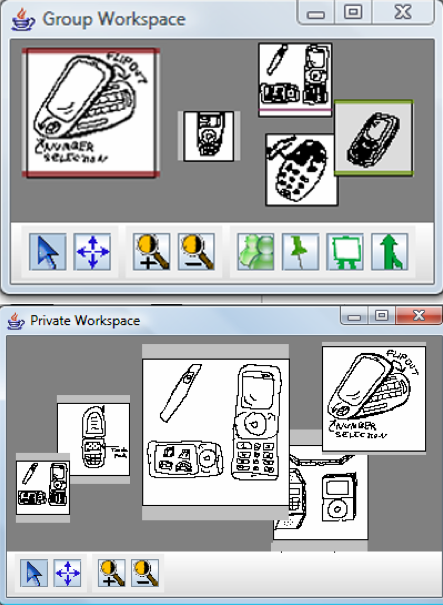
\includegraphics[width=\linewidth]{gfx/teamStormPrivateWorkspace.png}
	\caption{Gemeinsame und private Arbeitsbereiche in Team Storm. Designer können ihre Skizzen räumlich anordnen und die Größe anpassen.}
	\label{fig:teamStorm}
\end{figure}

Während ein Designer eine Skizze innerhalb des gemeinsamen Arbeitsbereichs überarbeitet oder ergänzt, sehen alle anderen Teilnehmer unmittelbar seine Änderungen. Die Gruppe kann auch gleichzeitig an unterschiedlichen Skizzen im gemeinsamen Bereich arbeiten.

Der gemeinsame Bereich wird nicht nur auf den Tablet-PCs der Designer, sondern auch auf einem großen, für alle sichtbaren Monitor dargestellt. Ähnlich wie ein Whiteboard, lädt diese Form der Darstellung dazu ein, sich davor hin zu stellen und Konzepte mit Hilfe zusätzlicher Kommunikationsformen, wie Gestik und Mimik, zu artikulieren. \autoref{fig:teamStormDisplayInteraction} zeigt, wie einer der Designer sich vor den Monitor stellt, um eine seiner Ideen zu erläutern.\\

\begin{figure}[bth]
	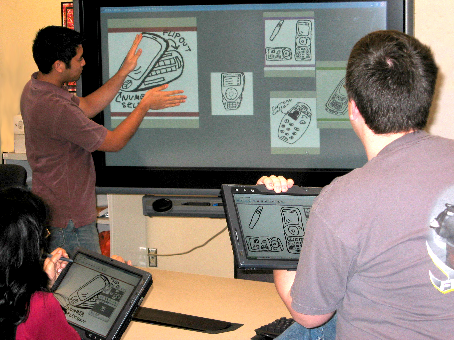
\includegraphics[width=\linewidth]{gfx/teamStormDisplayInteraction.png}
	\caption{Designer bei der Ausarbeitung von Konzepten mit Team Storm.}
	\label{fig:teamStormDisplayInteraction}
\end{figure}

Skizzen, die von einem Teilnehmer aus seinem privaten Arbeitsbereich in den gemeinsamen Bereich gezogen werden, befinden sich standardmäßig im Ausstellungsmodus. Das bedeutet, dass alle Designer die Zeichnung sehen, sie positionieren und skalieren, jedoch nicht ändern können. Sollte der Urheber der Skizze nicht wünschen, dass Größe und Position von seinen Kollegen nicht verändert werden dürfen, so kann er den Zugriff sperren. Er kann die Zeichnung jedoch auch ganz freigeben, sodass nicht nur Skalierung und Position für die Kollegen veränderbar sind. Um eine Zeichnung vom gemeinsamen Bereich zu entfernen, zieht der Designer sie wieder zurück in seinen privaten Arbeitsbereich.

Designer können freigegebene Skizzen direkt auf der gemeinsamen Arbeitsfläche modifizieren, damit die anderen Teilnehmer die Änderungen live mitverfolgen können. Zusätzlich gibt es die Möglichkeit, sich eine private Kopie zu erstellen, die ohne Einsicht der anderen Teilnehmer editiert werden kann. Dadurch können Designs in mehreren Iterationen editiert und verfeinert werden. Die unterschiedlichen Versionen nebeneinander angereiht zeigen die Evolution einer bestimmten Idee.

Die an Team Storm durchgeführte Studie \cite{Hailpern:2007p113} zeigt, dass Designer, die das erste Mal mit dem System arbeiteten, einen sehr einfachen und direkten Zugang zu dieser Groupware fanden. Es wurden sehr viele Ideen generiert und die Teilnehmer nutzten sehr stark die Features zur Organisation der Konzepte und Designs. Unterschiedliche Charaktere brachten unterschiedliche Arbeitsweisen zum Vorschein: einige Designer teilten offen jeden ihrer gezeichneten Striche mit, während andere es bevorzugten, Skizzen erst im privaten Bereich anzufertigen, um sie selbst zu evaluieren bevor sie sie herzeigten.

Die Gruppen nutzten das System auf sehr individuelle Art und Weise. Während manche hauptsächlich gemeinsam an einzelnen Designs arbeiteten, zogen andere es vor, parallel an verschiedenen Konzepten zu arbeiten, die dann gemeinsam evaluiert wurden.

Neben diesen positiven Eindrücken, kristallisierten sich auch einige mögliche Optimierungen des Systems heraus. Die Designer wünschten sich, Konzepte in Gruppen zu organisieren, die sie dann als Einheit positioniert, skaliert und hergezeigt hätten. Die Navigation wurde von vielen bei steigender Anzahl von Skizzen als ineffizient empfunden. Das System sah nur Scrolling und Zooming vor, die Teilnehmer wünschten sich hier weitere Möglichkeiten. Zusätzlich kam das Bedürfnis auf, andere digitale Artefakte (z. B. Bilder und Webseiten) einzubinden und dadurch Skizzen anzureichern.

%*****************************************
%*****************************************
%*****************************************
%*****************************************
%*****************************************

%\addtocontents{toc}{\protect\clearpage} % <--- just debug stuff, ignore
%*************************************************************
\chapter{Designtheorie}\label{ch:designTheorie} \index{Design!- theorie}
%*************************************************************

\begin{quote}
	\begin{flushright}{\slshape    
	    >>Schaut man sich die gegenwärtige Lage des Designs an, fällt der eklatante Widerspruch zwischen der Publizität des Desgignbegriffs - nach dem Motto ``Alles ist Design'' - und der Theorielosigkeit des Designs auf.<<} \\ \medskip
	    --- \defcitealias{Bonsiepe:1992}{Gui Bonsiepe}\citetalias{Bonsiepe:1992} \citep{Bonsiepe:1992}
	\end{flushright}
\end{quote}

Anders als in den meisten Professionen, kann die Disziplin \emph{Design} nicht verallgemeinert werden. Es muss stark zwischen der Theorie und der Praxis unterschieden werden. Wer nun eine allgemeine Theorie über Design erwartet, \emph{>>muss zur Kenntnis nehmen, dass eine solche Theorie nicht das intelligible Produkt eines Einzelnen sein kann, sondern allenfalls das Ergebnis einer Designdisziplin sein könnte, welche ihre Praxis reflektiert<<} \citep{Schneider:2008}.

\medskip Im folgenden Kapitel werden daher allgemeine Eigenschaften und Erklärungen von Design erläutert. Im Anschluss wird die Designpraxis, insbesondere von \ac{HCI} und Interaction Design, anhand modellzeigender Designmethoden erfasst.

\section{Was ist Design?} \index{Design}
Fragt man Fachleute verschiedener Abteilungen oder Berufsgruppen nach einer Definition von Design, so wird jeder eine andere Antwort finden. Geradezu jede Art der Kreation – vom Schreiben eines Programms bis zum Erstellen eines Businessplans – kann als Design verstanden werden. Durch diese Vielseitigkeit, ist es schwer eine präzise, nutzvolle Beschreibung zu finden.  Hier beginnt auch die Problematik. \citep{Sagmeister:2008}

\medskip John Heskett schrieb einst: \emph{>>Design is to design a design to produce design<<} \citep{Heskett:2005}. Dies zeigt, wie kompliziert und verwirrend eine Diskussion über Design durch den Begriff an sich bereits sein kann. Design hat so viele Bedeutungen, dass allein das Wort Verwirrung stiftet. Kritisch betrachtet, ist jedoch der Gebrauch des Wortes an jeder Stelle des Zitates grammatikalisch richtig. Das erste ist ein Nomen und beschreibt Design als generellen Überbegriff, wie z.B. in: >>Design ist wichtig für die Wirtschaft.<< Das zweite ist ein Verb und steht für eine Tätigkeit bzw. Prozess, wie z.B. in: >>Sie hat den Auftrag einen neuen Mixer zu designen.<< Das dritte ist wiederum ein Nomen, welches diesmal für ein Konzept bzw. einen Vorschlag steht, wie in: >>Das Design wurde dem Auftraggeber zur Freigabe vorgelegt.<< und das letzte ist wieder ein Nomen, das für ein fertiges Produkt steht, welches durch das Konzept umgesetzt wurde. Wie z.B.: >>Der neue VW Beetle lässt klassisches Design neu aufleben.<< \citep{Heskett:2005}\\
Durch diese Zerlegung kann man erkennen, dass sich der Begriff Design in zwei große Teilbereiche unterteilen lässt. Zum einen in die ursprüngliche Philosophie von Design - als Tätigkeit bzw. Prozess um ein Produkt zu entwickeln - und zum anderen in die Repräsentation eines Produkts. Webster beschreibt diesen Zusammenhang beider Bereiche wie folgt:
\begin{quote}
\slshape >>A design is an information base that describes aspects of this object, and the design process can be viewed as successive elaborations of representations, such as adding more information or even backtracking and exploring alternatives.<< 
\begin{flushright}\citep{Webster:1988}\end{flushright}
\end{quote}

\subsection{Design als Prozess} \index{Design!als Prozess}
Nach Webster ist der Designprozess eine schrittweise Ausarbeitung von Repräsentationen. Wann findet aber nun diese >>Ausarbeitung<< innerhalb eines Projektzyklus statt und was soll sie beinhalten?\\
Im Projektmanagement, welches sich mit der Gesamtheit an Aufgaben, Techniken, Mitteln etc. für die Abwicklung eines Projekts beschäftigt, spricht man dabei auch von der Designphase\index{Design!- phase}. Es gibt zwar Ansichten, dass die Designphase gleich der Entwicklungsphase ist, jedoch sind meist das die Projekte, die am Ende scheitern oder Schwierigkeiten haben, das Projekt in angegebener Zeit mit vordefiniertem Budget zu beenden.

\medskip Um ein Produkt zu entwickeln sollte man sich ausführliche Gedanken über die aufkommenden Probleme und um die Umsetzung zur Bewältigung dieser machen. Viele Projektmodelle wie z.B. das Wasserfallmodell\index{Wasserfallmodell} berücksichtigen bereits diesen Schritt. Jedoch gehen all diese Modelle von standardisierten Entwicklungsschritten aus, die zeitlich sequentiell durchlaufen werden sollen. Die Ergebnisse der Analyse- bzw. Forschungsphasen werden dabei in Dokumenten festgelegt um die weitere Entwicklung zu leiten und zu unterstützen. Das Zurückgreifen auf vergangene Phasen ist hier nicht erlaubt, jedoch in der Praxis die Regel und resultiert auf sog. >>Entwicklungsfehler<<.
Genau hier sollte das Umdenken beginnen. Die zwei (leider) gebräuchlichsten Mythen in der Industrie sind: 
\begin{quote}
	\begin{enumerate}
		\item \textsl{>>That we know what we want at the start of a project<<}, und
		\item \textsl{>>That we know enough to start building it<<.}
	\end{enumerate}
	\begin{flushright}\citep{Buxton:2007}\end{flushright}
\end{quote}

Die Realität sieht aber anders aus. Vor der Entwicklung werden einem nicht alle Probleme offenbart, welche im Projektverlauf auftreten, sondern lediglich Grundprobleme. Es ist im Vorhinein nicht möglich eine ganzheitliche Analyse durchführen ohne nicht auch Entscheidungen zu treffen, welche Analysen beeinflussen. Aus diesem Grund sollte der Designprozess durchgehend im Projektablauf verankert sein.
\autoref{fig:buxtonProductDevProcess} zeigt ein mögliches Modell eines Produktentwicklungsprozesses. Der	Designprozess	(in	rot gehalten) erstreckt sich hierbei über alle Phasen im Projekt bis zum Verkauf und beinhaltet das Design der Business- und Entwicklungspläne, sowie das Design des Produkts an sich. Plump	gesprochen ist die Hauptaufgabe	des	Designprozesses das Auffinden und Lösen von Problemen. Je nach Aufgabenstellung und Art des Projektes variieren naturgemäß die Probleme und somit auch die Aufgaben von Design als Tätigkeit. 

\begin{figure}
        {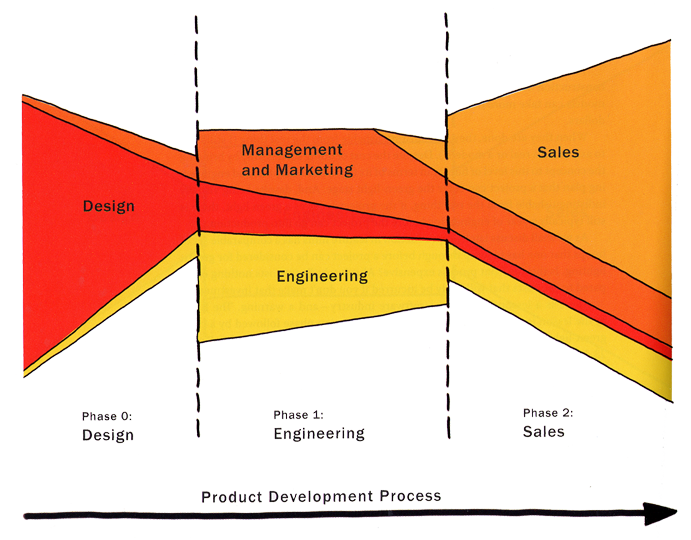
\includegraphics[width=\linewidth]{gfx/buxtonProductDevProcess}}
		\caption[Der Produktentwicklungsprozess \newline \citep{Buxton:2007}]{Der Produktentwicklungsprozess unterteilt in seine Verantwortungsbereiche. Von zentraler Bedeutung ist der Begriff Design, der das Design der Business- und Entwicklungspläne, sowie des Produkts selbst einschließt.}\label{fig:buxtonProductDevProcess}
\end{figure}

\subsection{Design als Repräsentation} \index{Design!als Repräsentation}
Das Entwickeln verwendbarer Repräsentationen eines Produkts ist essenziell im Designalltag. Repräsentationen können formal oder formlos, exakt oder vage sein und dienen verschiedenen Zwecken innerhalb des Designablaufs. Designer sollten zum einen die Fähigkeit besitzen eine passende Darstellung bzw. Repräsentation für ihre Aufgaben zu wählen, und zum anderen in der Lage sein diese auch richtig einzusetzen.
Im Laufe eines Produktdesigns können verschiedene Repräsentationen bzw. Modelle innerhalb des Designprozesses von Nöten sein. Ein gutes Modell ist präzise genug um die Eigenschaften des Systems wiederzuspiegeln, und einfach genug um Verwirrung zu vermeiden. Es verwendet eine Art der Repräsentation welche zum Zweck passt.
Die Wahl passender Modelle und das Konstruieren dieser, ist ein schwieriger aber wichtiger Teil der Arbeit von Designern. Sie müssen dabei stets beachten, wie das Modell verwendet werden soll und wer es benutzen wird. Deswegen sollte auch die Modellierungstechnik auf den Abstraktionsgrad und den >>Empfänger<< (der mit dem Modell arbeiten wird) angepasst werden. \citep{Preece:1994}
Wie im allgemeinen Produktdesign gibt es auch speziell im Softwaredesign eine große Menge an Repräsentationsarten bzw. Techniken, welche die Aufmerksamkeit auf verschiedene Aspekte des Designs lenken können. Auf diese Techniken, auch Designmethoden genannt, auf welches später eingegangen wird.

\subsection{Designdisziplinen} \index{Design!- disziplinen}
Design umfasst eine große Anzahl an verschiedenen Disziplinen. Sei es Produkt- bzw. Industriedesign, Kommunikationsdesign, Softwaredesign oder Modedesign, sie alle beinhalten auf ihrem Gebiet fachmännische Fähigkeiten und dienen zur Unterscheidung von Kompetenzen professioneller Designer. Über die Jahre kristallisierten sich ebenfalls die unterschiedlichsten Arbeitsfelder\index{Design!Arbeitsfelder} heraus. Das für Softwaredesign bedeutungsvollste der letzten Jahre ist (User) Interface Design bzw. Interaction Design, auf welche sich der folgende Text bezieht.\\
Um Interface Design beschreiben zu können, ist es vorerst nötig den Begriff des User Interfaces zu definieren. Das User Interface eines Systems besteht aus dem System selbst, dem Benutzer des Systems und der Weise, in der sie aufeinander einwirken. Es enthält somit Elemente die Teil des Systems sind, Elemente die ein Teil des Benutzers sind und Kommunikationsmethoden um Informationen von einem Ort zum anderen zu bringen.

\medskip Wie \autoref{fig:sagmeisterUI} zeigt, gibt es eine Grenze zwischen den Elementen des Systems, die Teile des User Interfaces sind und	denen, die für	die	internen Funktionen des Systems stehen. Das finden der passenden Grenze ist Aufgabe des	Designers und fällt	in den Aufgabenbereich	von	User Interface Design \citep{Barfield:1993}. Es befasst sich also mit der Entwicklung passender Benutzerschnittstellen zwischen Mensch und Maschine.

\begin{figure}
	\begin{center}
        {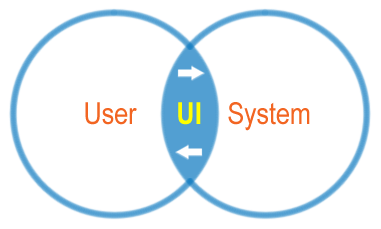
\includegraphics[width=.7\linewidth]{gfx/sagmeisterUI}}
	\end{center}
		\caption[Visualisierung des User Interfaces \newline \citep{Sagmeister:2008}]{Visualisierung des User Interfaces. Das User Interface, welches aus dem System und dem Benutzer geformt wird, stellt Methoden zu Verfügung um die Kommunikation beider Seiten bestmöglich zu unterstützen. Das Finden einer passenden Grenze von Funktionen, die zum Interface oder intern zum System gehören, ist Aufgabe von User Interface..}\label{fig:sagmeisterUI}
\end{figure}

\medskip Interaction Design beschäftigt sich ähnlich wie Interface Design mit dem Verhalten von Mensch und Maschine. Jedoch spezialisiert es sich auf die Wechselwirkungen bzw. Interaktionen zwischen Menschen, welche durch Verbindungen mit maschinellen Produkten entstehen. Der Zusammenhang zwischen User Interface Design/Engineering bzw. Interaction Design ist in \autoref{fig:safferInteractionDisciplines} ersichtlich. Sie zeigt ebenfalls verwandte Disziplinen, wie \emph{Information architecture}, \emph{Communication design}, \emph{Usability engineering} oder \emph{Human-computer interaction}, welche sie nicht nur beeinflussen, sondern auch Teil von ihnen sind. Man merkt somit wie schwierig es ist, Disziplinen, die zwar separat existieren aber sich mit vielen anderen Disziplinen überschneiden, abzugrenzen und ihre Funktionen zu beschreiben. Nicht jede Organisation benötigt einen Spezialisten für jede Disziplin. Eine Person, möge er sich Informationsarchitekt oder Interface Designer nennen, kann und wird höchstwahrscheinlich in mehreren Disziplinen, je nach Bedarf tätig sein. \citep{Saffer:2007}

\begin{figure}
	\begin{center}
        {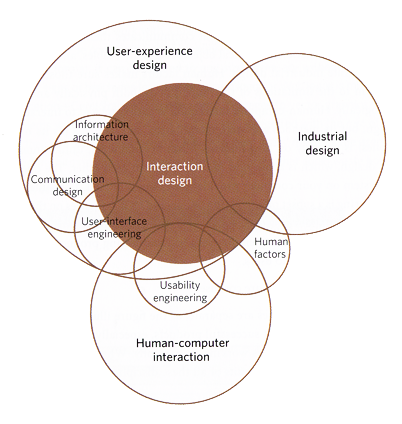
\includegraphics[width=.8\linewidth]{gfx/safferInteractionDisciplines}}
	\end{center}
		\caption[Verwandte Disziplinen von Interface- und Interaction Design \newline \citep{Saffer:2007}]{Verwandte Disziplinen von Interface- und Interaction Design. Sie beeinflussen nicht nur, sondern sind auch Teil von Interface bzw. Interaction Design. Die Schwierigkeit	Disziplinen abzugrenzen, zeigt den interdisziplinären Charakter, den Designer an den Tag legen.}\label{fig:safferInteractionDisciplines}
\end{figure}

\medskip Zu diesen zählen ebenfalls andere akademische Disziplinen, wie z.B. im sozialen, technologischen oder organisatorischen Sektor, wie \autoref{fig:benyonDisciplines} veranschaulichen soll.\\
Natürlich ist es nicht nötig, dass Designer alle Fähigkeiten zur Erstellung von Designs besitzen - vor allem da das Designen von Interaktiven Systemen meist Aufgabe eines ganzen Teams ist - jedoch müssen sie in der Lage sein, Techniken anderer Disziplinen	anwenden	zu können bzw. wenn nötig die Mittel zur Erforschung dieser besitzen. \citep{Benyon:2005}

\begin{figure}
        {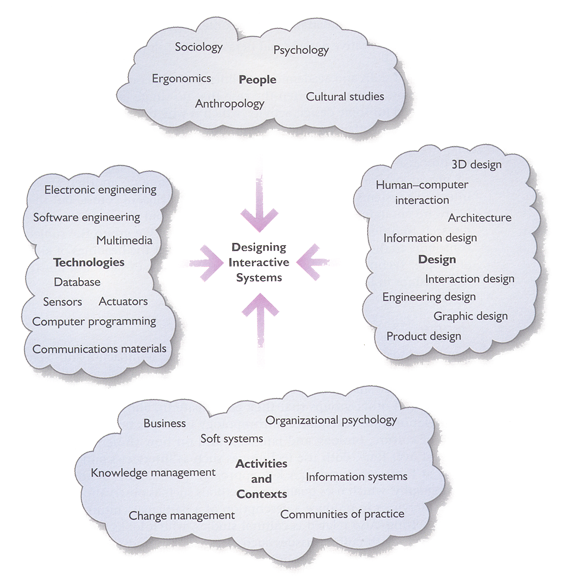
\includegraphics[width=\linewidth]{gfx/benyonDisciplines}}
		\caption[Miteinfließende Disziplinen im Interaktiven System Design \newline \citep{Benyon:2005}]{Miteinfließende Disziplinen im Interaktiven System Design. Sie verkörpern Bereiche aus welchen Designer Techniken beziehen	und anwenden. Es ist zwar nicht nötig, dass Designer jeweils alle Fähigkeiten besitzen müssen, jedoch sollten sie wenn nötig die Mittel zur Erforschung dieser besitzen.}\label{fig:benyonDisciplines}
\end{figure}

\medskip Im Allgemeinen lässt sich aber User Interface- bzw. Interaction Design wie folgt beschreiben:

\begin{quote}
	\textsl{>>The design of the subjective and qualitative aspects of everything that is both digital and interactive.<<}
	
	\smallskip oder allgemeiner: 
	\smallskip
	
	\textsl{>>The design of everything that is both digital and interactive.<<}
\begin{flushright}\citep{Moggridge:2007}\end{flushright}
\end{quote}

\subsection{Der kollaborative Charakter} \index{Design!- kollaboration}
Designkollaboration wird durch die soziale Welt geformt. Aus diesem Grund ist es unmöglich Designspezifikationen und Artefaktbeschreibungen zu interpretieren, ohne die soziale Situation in der sie erstellt wurden zu verstehen \citep{Brown:2002}. Da Design immer mit Kommunikation und Interaktion - zwischen Einzelpersonen und Gruppen in komplexen sozialen Situationen - zusammenhängt, können die technischen Ergebnisse nicht vom sozialen Charakter der Designaktivitäten getrennt werden. Er ist durchgehend in Meetings, Diskussionen, Argumenten, Debatten und Interpretationen vorhanden und macht das dichtverflochtene Gewebe von Design aus. Minneman beschreibt in diesem Zusammenhang Design als \emph{>>social contruction of a technical reality<<} \citep{Minneman:1991}.

\medskip Kollaborative Wissenskonstruktion ist wichtig für ein erfolgreiches Design. Zudem ist es auch wichtig, Mehrdeutigkeiten zu bewahren, um Teammitglieder Freiheiten zu ermöglichen.

\begin{quote}
	\textsl{>>[It is important to provide team members with] the freedom to manoeuvre independently within objects worlds and providing room for the recasting of meaning in the negotiations with others.<<}
\begin{flushright}\citep{Bucciarelli:1994}\end{flushright}
\end{quote}

\medskip Eine erfolgreiche Kollaboration zeichnet sich durch die Bildung eines gemeinsamen Verständnisses aus. Clark und Brennan benutzen den Begriff \emph{Grounding} um diesen Vorgang zu beschreiben, in dem das Kommunizierte auch verstanden wird. Sie erklären weiters: \emph{>>all collective actions are built on common ground and its accumulation<<}, womit sie betonen, dass Gemeinsamkeiten kontinuierlich von Moment zu Moment durch die Interaktion der Teammitglieder aufgebaut werden \citep{Clark:1991}. Diese Interaktionen treten in verschiedenen Formen auf und beeinflussen den kollaborativen Designprozess. Short et al. nennen in \citep{Short:1991} beispielsweise Aspekte der visuellen Kommunikation, welche soziale Interaktionen beeinflussen: 

\begin{quote}
	\textsl{>>In normal face-to-face interaction, the participants exchange in addition to the verbal material, a range of non-verbal cues such as facial expression, direction of gaze, posture, dress and physical distance.<<}
\begin{flushright}\citep{Short:1991}\end{flushright}
\end{quote}

Um also ein Verständnis über Designkollaboration zu bekommen, müssen Gemeinsamkeiten, in Hinsicht auf Relevanz und Bedeutung der in kollaborativen Designaktivitäten vorgebrachten Informationen, erlangt werden \citep{Hill:2001}.

\subsection{Designvokabular} \index{Design!- vokabular}
In einer Studie über Industrial Designer, die an Konzeptskizzen arbeiteten, fanden Pan et al. \citep{Pan:2002} heraus, dass die Designer die Formen ihres Designs auf verschiedene Weisen verbal beschrieben. Ihre Sprache war nicht klar, einheitlich oder im Allgemeinen verständlich für Außenstehende. Designer haben ein \emph{>>creative vocabulary, which has rich meanings in design communication<<}\citep{Pan:2002}. In Hinsicht auf globale Kollaborationen zwischen einzelnen Arbeitsgruppen, ist der Wunsch an ein gemeinsames Designvokabular naheliegend. Laut Hill \citep{Hill:2001} baut der Erfolg von Designteams stark auf die folgende Fähigkeit der Teilnehmer auf: \emph{>>negotiate different design perspectives and specialities<<}. \emph{>>Similarities in voice<<} ist das Um und Auf, bei Teammitglieder mit verschiedenen Disziplinen und Hintergründen.

\medskip Das Definieren eines gemeinsamen Designvokabulars scheint aber doch eher utopisch. Bucciarelli meinte dazu, dass auch wenn Teilnehmer die gleiche gemeinsame Sprache (wie z.B. Englisch) verwenden, kann die Sprache auf verschiedene Weisen angewendet werden, wodurch es scheint als würde ein Teilnehmer einer andere Sprache sprechen:

\begin{quote}
	\textsl{>>Not different in the sense that for you, as a foreigner, a translation would make meanings clear \ldots but different in that the concepts and ideas and relationships among the things of an opbject world require new leaning, like the learning of a foreign language.<<}
\begin{flushright}\citep{Bucciarelli:2002}\end{flushright}
\end{quote}

Im Grunde bedeutet dies für Designteams (speziell für globale), dass sie nicht nur eine sprachliche Hürde von z.B. Personen unterschiedlicher Herkunft meistern müssen, sondern auch von Personen, die von komplett unterschiedlichen Objektwelten stammen - abhängig von kulturellen Hintergrund, der Ausbildung und professionellen Disziplinen.

\medskip Larsson hält \emph{Negotiation} als adequateren Begriff, um die Kommunikation zwischen den einzelnen Mitgliedern eines Designteams zu beschreiben, da die Teilnehmer aktiv den Kontext und Inhalt der Situationen formen und die Informationen nicht passiv mit eindeutigen Bedeutungen und definierten Settings übertragen. \citep{Larsson:2003} \\
Die Wissenskonstruktion ist ein kollaborativer Prozess, der wie bereits Bucciarelli beobachtete, aus einer inhärenten Mehrdeutigkeit besteht, welche Designer vor die folgende, alles andere als einfache Aufgabe stellt: 

\begin{quote}
	\textsl{>>frequently bringing the results of their object world efforts, which no doubt will conflict, into coherence if design is to proceed - and they must do this without a shared proper language.<<}
\begin{flushright}\citep{Bucciarelli:2002}\end{flushright}
\end{quote}

\subsubsection{Storytelling} \index{Storrytelling}
Eine Art um Verständnis unter Designern zu vermitteln, ist das Erzählen von Geschichten. Geschichten ermöglichen Designer gezielter zu erklären, was sie gerade machen, im Gegensatz zu dem was sie machen sollten - falls sie sich an normative Designmodelle halten. Auch wenn die Geschichten nicht direkt ein Problem lösen, helfen sie dennoch ein gemeinsames Vokabular aufzubauen, um über das Design sprechen zu können. Sie kreieren \emph{>>a new language capable of describing aspacts of the evolving design<<} \citep{Lloyd:2000}.

\medskip Vereinbarte Geschichten ermöglichen Designer verschiedener Sparten, ein gemeinsames Verständnis zu kreieren, auf das sie sich beziehen können, ohne dabei zu konkreten Thematiken zustimmen zu müssen. Es sind konkrete Beispiele, auf die sich Personen mit verschiedenen Hintergründen beziehen können. Da uns das formlose Naturell von Geschichten dazu bringt sie nicht zu ernst zu nehmen, dienen sie als eine gemeinsam verfügbare Wissensquelle - die Freiraum für Interpretation und Fragestellungen aller Beteiligten zulässt \citep{Erickson:1996}. Wie in Orrs Studie über Service Techniker \citep{Orr:1986} beobachtet wurde, dienen Geschichten auch dem Zweck, Erfahrungen zu erhalten und zu verbreiten. Somit bieten sie Grundgerüst für Problemlösungsaktivitäten.

\medskip Zusätzlich bilden sie ein Transportmittel für Gedanken, da sie durch ihre Nutzung, nicht nur anderen etwas beschreiben, sondern auch uns selbst \citep{Norman:1994}.

\subsubsection{Indexical Expressions} \index{Indexical Expressions}
Neben Geschichten, die nützlich bei der Verständnisvermittlung sind, benutzen Designer auch \emph{Repräsentationen}, wie Markierungen oder Symbole, die etwas bestimmtes darstellen und ihnen bei ihren Argumentationen helfen \citep{Norman:1994}. Repräsentationen bieten auf die gleiche Weise wie Geschichten konkrete Beispiele, welche die Gedanken der Designer abbilden. Dabei benutzen sie vorhandene Tools, die die Verständnisvermittlung zwischen den Teammitgliedern im jeweiligen Moment am besten unterstützen.

\medskip In Hinsicht auf ein gemeinsames Designvokabular muss man zur Kenntnis nehmen, dass einige Teile des Vokabulars keine strikten Definitionen haben. Designer und auch andere Personen, benutzen \emph{Indexical Expressions} wenn sie kommunizieren. Eines muss man sich dabei aber vor Augen halten:

\begin{quote}
	\textsl{>>[Indexical Expressions] cannot straightforwardly be repeated or reused outside the context in which they originated, without changing their meaning.<<}
\begin{flushright}\citep{Kristoffersen:1999}\end{flushright}
\end{quote}

Beispielsweise \graffito{Markierungen und Symbole verlieren außerhalb des Kontextes ihre Bedeutung.} können Wörter wie >>hier/dort<<, >>dies/das<<, >>sein/seine<< oder >>jetzt/dann<< nicht angemessen gedeutet werden, ohne zu wissen unter welchen Umständen sie benutzt wurden \citep{Larsson:2003}.

\medskip Designvokabular dient aber nicht nur zur Verständigung, sondern ist vielmehr ein Hilfsmittel, das Designer bei ihren Arbeitsmethoden begleitet und mit diesen zusammenspielt. \emph{Storytelling} und \emph{Indexical Expressions} deuteten bereits auf essentielle Designmethoden hin, welche im folgenden Abschnitt genauer betrachtet werden.

\section{Designmethoden} \label{sec:designmethoden} \index{Design!- methoden}
Vorstellungskraft ist grundlegend für effektive Designarbeiten. Sie hilft, Dinge aus einem anderen Blickwinkel zu sehen und Designkonzepte bzw. Ideen mit anderen zu erforschen. Verschiedenste Repräsentationen von Designideen können in verschiedenen Etappen für verschiedene Menschen nützlich sein und ihre Vorstellungen beeinflussen. Sie helfen beim Finden, Austauschen und Auswerten von Ideen.

\medskip Es gibt viele Techniken bzw. Methoden, die benutzt werden können um Designprobleme zu verstehen und mögliche Lösungen zu entwickeln. Keine dieser Methoden führt höchstwahrscheinlich zum perfekten Design, aber zu einer Art Dokument oder Darstellung, die benutzt werden kann um sich besser mit Auftraggebern, Benutzern und Kollegen zu verständigen. Verständigung ist es auch, wodurch Lösungen entstehen, ausgewertet, und eventuell zum Endprodukt umgewandelt werden \citep{Benyon:2005}.

\medskip Es werden im folgenden nun wichtige Methoden und Hilfsmittel für Designer beschrieben und Einblicke über deren Grundfunktionsweise geboten. Welche Techniken aber in einem Projekt tatsächlich Anwendung finden, hängt von mehreren Faktoren ab: die Herangehensweise an die Arbeit des Entwicklungsteams, die Art des Projekts, die zur Verfügung stehenden Hilfsmittel etc. Das Auswählen von passenden Methoden bzw. Repräsentationen ist Aufgabe des Designers und erfordert Geschick, um sie auch gut einsetzen zu können. Dabei sollte aber nicht die Repräsentation an sich, sondern die Vorstellungskraft und das Verständnis im Vordergrund stehen, geistig und vor allem erfahrungsmäßig. \citep{Sagmeister:2008} 

\begin{quote}
	\textsl{>>Experience is a very dynamic, complex and subjective phenomenon. It depends upon the perception of multiple sensory qualities of a design, interpreted through filters relating to contextual factors. For example, what is the experience of a run down a mountain on a snowboard? It depends upon the weight and material qualities of the board, the bindings and your boots, the snow conditions, the weather, the terrain, the temperature of air in your hair, your skill level, your current state of mind, the mood and expression of your companions. The experience of even simple artefacts does not exist in a vacuum but, rather, in dynamic relationship with other people, places and objects.<<}
\begin{flushright}\citep{Buxton:2007}\end{flushright}
\end{quote}

\subsection{Artefakte} \index{Artefakte}
Harrison und Minneman beobachteten in \citep{Harrison:1996}, dass Objekte wesentliche Bestandteile von Designkommunikation sind, da sie einen Teil des \emph{Repräsentationspools} von Designer ausmachen. Diese Objekte oder auch Artefakte genannt, können praktisch alles sein; z.B. ein Stift, ein Sessel, eine Zeichnung, oder ein einfaches Blatt Papier. Im Konzeptdesign sind diese besonders wichtig, da in diesem Stadium des Produktentwicklungsprozess noch kein >>gemeinsames<< Designobjekt existiert \citep{Tuikka:2001}. Aus diesem Grund muss ein gemeinsames Artefakt erst durch Kollaboration konstruiert werden, um Diskussionen über Designoptionen und Ideen zu ermöglichen. \citep{Larsson:2003}

\medskip Artefakte sind ein bewehrtes Mittel in \ac{HCI} und \ac{CSCW}. Verschiedene Studien zeigen, das sie eine große Rolle in kooperativen Arbeiten spielen (vgl. \citealp{Bardram:2005, Heath:1992, Hutchins:1995, Robinson:1993, Schmidt:2002, Sellen:2003, Shapiro:1994, Vyas:2008}). Die Forschung und Literatur (z.B. \citealp{Randall:2007}) beschäftigt sich dabei vorwiegend mit drei Hauptaspekten im Bezug auf Artefakte bei der Arbeit: dem \emph{ökologischen}, dem \emph{koordinativen} und dem \emph{organisatorischen}.

\medskip \emph{Ökologisch.} Die Umwelt von Artefakten kann einiges über die Arbeitspraktiken von Personen aussagen. Der Ort, die Position, der Aufbau und die Ausrichtung der Artefakte erlaubt uns zu verstehen was und wie gearbeitet wird. Verschiedene \ac{CSCW} Studien \citep{Heath:1992, Sellen:2003} zeigten, dass die Organisation des Arbeitsbereiches Auswirkungen auf die Arbeit haben. Kidd \citep{Kidd:1994} zeigte, dass die ökologische Struktur von Artefakten eine >>primitive Sprache<< bildet, welche Arbeit erklärt. Er vertritt den Standpunkt, dass die persönliche Anordnung von Artefakten (wie z.B. Papier), Personen befähigt ein besseres Verständnis aufzubauen, da sie so ein Gesamtbild ihrer Arbeit bekommen. Ebenso werden Aufbewahrungsmöglichkeiten, wie z.B. Papierstapel oder -mappen, zu externen Repräsentation, die zusätzliches Verständnis vermitteln und bewahren. Der physische Kontext und die Positionierung geben Artefakten oder ihrer Aufbewahrung eine >>Bedeutung<<. Somit spiegelt der ökologische Aspekt eines Artefakts einige Vorgänge wieder, die zum Verständnis von Arbeitspraktiken beisteuern können.

\medskip \emph{Koordinativ.} Verschiedenste Variationen von Artefakten, welche im Arbeitsbereich, zu Hause oder sonst wo benutzt werden, können als Wissensvermittler dienen. Flugstreifen\footnote{Flugstreifen, engl. \emph{Flight (Progress) Strips}, werden in der Luftraumüberwachung eingesetzt. Die noch üblicherweise in Papier gehaltenen Streifen beinhalten wichtige Informationen zu allen derzeitigen und zukünftigen Flügen. \citep{Bentley:1992}}(vgl. \citealp{Shapiro:1994}), Pinnwände (vgl. \citealp{Bardram:2005}) oder Papierdokumente (vgl. \citealp{Sellen:2003}), zeigten beispielsweise schon in der Vergangenheit, dass wichtige Arbeitsschritte durch Artefakte koordiniert werden. Ein Papierartefakt kann eine bleibende Informationsform sein, oder auch ein Medium, welches von einem Arbeitsbereich zum nächsten wandert, um kollaboratives Arbeiten unter Mitarbeitern zu unterstützen. Sellen und Harper untersuchten in \citep{Sellen:2003} die unterschiedlichen Merkmale von Papier und zeigten, dass dessen physikalische Eigenschaften verschiedene menschliche Handlungen - wie greifen, herumtragen, falten oder darauf schreiben - ermöglichen. Sie fungieren durch ihre weitgehende Verfügbarkeit \citep{Heath:1992} und Verteilung \citep{Robinson:1993}, als Koordinationstool mehrerer Personen, die an gemeinsamen Projekten arbeiten \citep{Vyas:2008}. Gemeinsamkeiten können somit durch physikalische Objekte einfacher erarbeitet werden, als durch verbale Kommunikation alleine \citep{Larsson:2003}.

\medskip \emph{Organisatorisch.} Wie lange ein Artefakt an einem Arbeitsbereich benutzt wird, sagt viel darüber aus, wie die Arbeit organisiert ist. In einem Betrieb, wandert Information durch verschiedene Darstellungsformen. Ein Artefakt, im speziellen dessen raum-zeitlicher Aspekt, kann somit Auskunft über wichtige Prozesse, Protokolle oder Konventionen eines Arbeitsvorgangs geben. Schmidt und Wagner zeigen in \citep{Schmidt:2002}, dass \ac{CAD} Zeichnungen als mehrlagiges Artefakt, die Koordination und Organisation mehrerer verschiedener Aktivitäten erleichtern kann. Eine \ac{CAD} Zeichnung mit einer Mischung aus Chiffren für Funktionen und Materalien, könnten so beispielsweise auch Details über Verantwortungsbereiche einer Arbeit veranschaulichen. Kidd zeigt in \citep{Kidd:1994}, dass durch die fühlbaren raum-zeitlichen Aspekte der Artefakte (wie z.B. Papierstöße), Arbeitsfortschritte gemessen werden können. \citep{Vyas:2008}

\bigskip Die tatsächlichen Eigenschaften von Artefakten müssen zwangsweise nicht optimal oder vollkommen geeignet sein um das Denken von Designer zu unterstützen. In einer Studie über die Benutzung von Artefakten von Designstudenten, erkannte Brereton \citep{Brereton:2000}, dass es im Vorhinein nicht möglich ist, das >>richtige<< Artefakt für eine Designsituation zu bestimmen:

\begin{quote}
	\textsl{>>The hardware was simply conveniently available and had some attribute that meant students found it helpful to gesture and think with.<<}
\begin{flushright}\citep{Brereton:2000}\end{flushright}
\end{quote}

\subsubsection{Conversational Props} \index{Conversational Props}
Der beabsichtigte Zweck von Artefakten, das Verständnis essentiell zu fördern, bedeutet dass Designer Objekte suchen, die ihnen helfen ihre eigenen Gedanken zu formen und diese den anderen Teilnehmern eines Designteams zu vermitteln. Diese Objekte werden auch \emph{Conversational Props} \citep{Brinck:1992} genannt, da mit ihnen ein Element der Realität zu einer Konversation hinzufügt wird. \citep{Larsson:2003}

\subsubsection{Boundary Objects} \index{Boundary Objects}
Artefakte können auch als Mediatoren zwischen verschiedenen Personen oder Gruppen dienen, indem sie das Terrain werden >>on which conflicts and collaboration occur<< \citep{Perry:1998}. Bei Gruppenmitglieder verschiedener Disziplinen, mit unterschiedlichen Interessen und Zielen werden Artefakte als sog. \emph{Boundary Objects} \citep{Star:1989} angesehen und benutzt. Sie sind nützliche Repräsentationen für alle Gruppenmitglieder, haben aber möglicherweise noch zusätzliche Bedeutungen für jeden einzelnen. \citep{Larsson:2003}

\begin{quote}
	\textsl{Boundary Objects >>have different meanings in different social worlds but their structure is common enough to more than one world to make them recognizable, a means of translation.<<}
\begin{flushright}\citep{Star:1989}\end{flushright}
\end{quote}

Laut Bucciarelli \citep{Bucciarelli:2002} sind Boundary Objects oder gemeinsame Artefakte auch für Teilnehmer gleicher Disziplinen essentiell, da die analytische Natur einer Sprache meist nicht ausreicht.
\begin{quote}
	\textsl{>>[Language] hardly allows \ldots the kind of experimentation and innovative thinking that designing requires.<<}
\begin{flushright}\citep{Bucciarelli:2002}\end{flushright}
\end{quote}

\subsection{Skizzieren} \index{Skizzen}
Die Kunst des Skizzierens ist eine Fähigkeit, die jeder Designer beherrschen sollte. Ideen und Gedanken können schnell veranschaulicht und erforscht werden - entweder für sich selbst oder für andere. \citep{Sagmeister:2008} 

\medskip Donald Schöns Beobachtungen zeigten, dass Designer beim Skizzieren eine Wechselbeziehung mit ihren Zeichnungen eingehen. Er nennt dies \emph{>>conversation with the materials of the situation<<} \citep{Schoen:1983}, womit er den Vorgang beschreiben will, in der Designer etwas zeichnen, dann ihre Skizze interpretieren und wieder weiter zeichnen. Den selben Prozess beobachtete auch Gedenryd, in dem Designer durch wie er es nennt >>stepwise reasoning-by-drawing<< nachdenken und neue Ideen generieren \citep{Gedenryd:1998}.

\subsubsection{Warum skizzieren?} 
Skizzen sind ein Weg um Ideen offenzulegen, eigene Gedanken zu veröffentlichen oder flüchtige Gedanken zu fixieren. Wörter können zwar das selbe, aber Skizzen haben den Vorteil bildliche Gedanken direkt zu vermitteln. Benutzte Elemente und räumliche Relationen auf Papier verdeutlichen Elemente und räumliche Relationen in der Realität. Das könnte auch ihre Allgegenwart erklären; Landkarten und architektonische Pläne wurden in verschiedenen Kulturen überall auf der Welt in Stein geritzt, in Leder gebrannt, in Ton geprägt und auf Papier gezeichnet. Skizzen können ebenfalls abstrakte Ideen metaphorisch beschreiben, wo Elemente und räumliche Relationen auf Papier, abstrakte Elemente und Relationen ausdrücken. Das Äußern von Ideen in einem bildhaften Medium macht Verständnis und Folgerung einfacher als in einem abstrakten Medium wie Sprache. Die Klarheit von Skizzen und gleichartigen kognitiven Werkzeugen treibt das Erinnerungsvermögen an, in dem sie etwas liefern, das nicht nur auf das unzuverlässige Gedächtnis des Menschen vertraut. Sie bieten ebenso ein Souvenir an frühere Gedanken, in dem sie gleichzeitig den Inhalt und dessen Bedienung vermitteln. Die öffentliche Natur von Skizzen erlaubt einer Gemeinschaft Ideen zu beobachten, zu kommentieren, oder zu ändern - und dies in der Repräsentation festzuhalten.

\medskip So wie Sprache (gesprochen oder geschrieben), sind Skizzen eine Form von Kommunikation. Aber anders als Sprechen, dienen Skizzen auch zur Kommunikation mit sich selbst. Eine Aufgabe von Skizzen ist die Vollständigkeit und interne Konsistenz einer Idee - im Besonderen räumliche Ideen - zu prüfen. Eine Skizze ist ein schriftliches Modell einer Idee, eine Existenzüberprüfung. Eine weitere Aufgabe ist neue Relationen und Formen für sich selbst zu entdecken, welche zu neuen Ideen führen können. Skizzen werden mit einer bestimmten Ausgangsidee und einem Ziel begonnen, enden aber meinst durch Zufall in neuen Objekten und Konfigurationen. Dies führt zu unbeabsichtigten Entdeckungen und kann eine fruchtbare Quelle für neue Designideen sein. \citep{Tversky:2002}

\medskip Goel geht einen Schritt weiter und versucht konkrete Eigenschaften für Skizzen zu formulieren: \index{Skizzen!Eigenschaften}
\begin{enumerate}
	\item Die dichte Anordnung von einzelnen Skizzen, die sich vielleicht auch nur gering unterscheiden, hilft eine Skizze gegebenenfalls in eine andere umzuwandeln und das Ausschließen von Möglichkeiten im Vorhinein zu unterbinden.
	\item Die Mehrdeutigkeiten von Skizzen versichern, dass die Darstellungen bzw. auch Inhalte während der frühen Phasen des Designs unbestimmt bleiben. Das ist wichtig, um die Entwicklung des Designs durch Konkretisieren von Ideen nicht zu früh zu blockieren.
	\item Die dichte Anordnung von inhaltlich ähnlichen Skizzen, oder auch Skizzen der gleichen Bezugsquelle versichern, dass Möglichkeiten nicht ausgeschlossen werden, um Ideen in andere umzuwandeln.
\end{enumerate}
\begin{flushright}\citep{Goel:1995}\end{flushright}

\subsubsection{Was beinhalten Skizzen?} \index{Skizzen!Inhalte}
\emph{Schematische Strukturen.} Das beste und weitverbreiteste Beispiel dafür sind Landkarten und Wegbeschreibungen. Sie beinhalten wichtige Informationen zu ihrem Zweck und eliminieren die unwichtigen. Darüber hinaus vereinfachen und verzerren sie sogar die Informationen, um einer bestimmten Struktur zu entsprechen. Die Struktur, die mit den Skizzen eingefangen wird, ist nicht die Struktur der Umwelt, sondern eine konzeptuelle Struktur der Information. Wie Sprache, bestehen Skizzen aus Elementen. Diese können vereinfachte Figuren, Linien, Kurven und tropfenartige Gebilde sein \citep{Tversky:2000}. Diese Elemente können in verschiedenen Weisen kombiniert werden um verschiedene, sprachähnliche, Bedeutungen zu erlangen \citep{Goodman:1968}.

\medskip \emph{Hierarchische Strukturen.} Skizzen von Regionen zeigen z.B. andere Charakteristiken. Die Reihenfolge in der Personen Landkarten zeichnen, spiegelt die konzeptuelle Struktur der Karten wieder \citep{Taylor:1992}. Versuchen Teilnehmer eine gesehene Karte zu reproduzieren, bleibt die Reihenfolge der Elemente gleich. Das zeigt, dass Personen hierarchische Strukturen aufbauen um die Umwelt zu strukturieren \citep{Tversky:2002}.

\medskip Skizzen sind keine Präsentationen der Realität, sondern Repräsentationen der Realität \citep{Tversky:1999}. Sie unterschieden sich von der Realität auf folgenden Arten: sie lassen bestimmte Informationen weg, fügen Informationen hinzu und verzerren Informationen. Somit sind sie keine Bilder, zumindest nicht im >>klassischem<< Sinne \citep{Kosslyn:1980}. Skizzen können vielmehr Abbildungen von Ideen sein. Als solche können sie Ideen - besonders bildhafte - effektiv vermitteln.

\subsubsection{Was gewinnt man aus Skizzen?} \index{Skizzen!Verwertung}Man kann nicht garantieren, dass Personen Skizzen so verstehen, wie sie der Macher beabsichtigte. Häufig sind sie selbst für denjenigen, der sie angefertigt hat ein Rätsel, wenn er sie nach langer Zeit erneut betrachtet. %Wie oft haben wir unsere eigenen Skizzen und Schreibereien nach längerer Zeit wieder angesehen, und waren verdutzt darüber, was wir damit ausdrücken wollten. 
In zahlreichen Bereichen, mitunter bei Karten und Gerätedarstellungen, wird versucht eine Struktur zu vermitteln. Die Struktur einer Route kann durch eine gut gezeichnete Wegbeschreibung, genauso wie die Struktur eines Gerätes, durch eine gute schematische Darstellung entnommen werden \citep{Heiser:2002}.

\medskip Skizzen bieten Designer, wie bereits erwähnt eine Quelle für neue Ideen. Skizzen und Diagramme können auch nützlich sein um mehr als nur eine Struktur zu vermitteln. Sie sind auch ein effektives Mittel um bestimmte Abstraktionen zu verdeutlichen, welche von der Struktur gefolgert werden und keinen direkten Zusammenhang mit der Skizze an sich haben. Gute Beispiele hierfür wären eine Fahrradpumpe, die Bremsen in einem Auto oder ein Flaschenzug. All diese Dinge sind in Bewegung, bzw. bewegen sich um einen bestimmten Zustand zu erreichen. Wie sie sich bewegen und was ihr Ziel ist, wird üblicherweise nicht direkt in den Skizzen verdeutlicht. Das Hinzufügen eines Pfeiles hingegen, ändert ihre Interpretation.

\begin{quote}
	\textsl{>>When asked to write descriptions of what is portrayed in the diagram, participants viewing simple diagrams of a car brake, pulley system or bike pump write structural descriptions. When arrows were added to the diagrams, participants write functional descriptions of the devices, explaining what they do, step-by-step.<<}
\begin{flushright}\citep{Tversky:2002}\end{flushright}
\end{quote}

Pfeile vermitteln zeitliche Abläufe und erlauben den Betrachtern ein Gerät gedanklich zu animieren \citep{Hegarty:1992}.

\subsubsection{Sketching for Experience} \index{Sketching for Experience}

Egal ob Designer zeichnen oder schreiben, die besten Werkzeuge dafür bleiben Stift und Papier. Kein digitales Medieum war bis jetzt in der Lage, die Flexibilität, die Geschwindigkeit und die Mühelosigkeit des Skizzierens auf Papier oder Whiteboard zu überbieten \citep{Sagmeister:2008}. Warum das so ist, soll in \autoref{ch:DesignVSComputer} erörtert werden.

\medskip Eine weitere bewährte Form des Skizzierens ist Modellierung. \index{Modellierung}Modelle können durch eine Vielzahl an Materialien, von Ton bis Styropor gebildet werden und bieten somit dreidimensionale Repräsentationen (siehe \autoref{fig:vyasModelle}). Modelle wie Skizzen, können in einem kurzen Zeitraum schnell zusammengefügt werden, um grobe Annäherungen von Gegenständen und Umgebungen zu erstellen. Die Unbestimmtheit dieser, die auch schon Goel erwähnte, führt dazu, dass die Betrachter sich in ihrer Kommentierfunktion uneingeschränkt fühlen und stets neue Ideen und Anregungen einbringen.

\medskip Bill Buxton spricht bei dieser Art von Skizzen (dies inkludiert auch Modellierung) von \emph{Sketches for Experience}: 
\clearpage
\begin{figure}
	\begin{center}
        {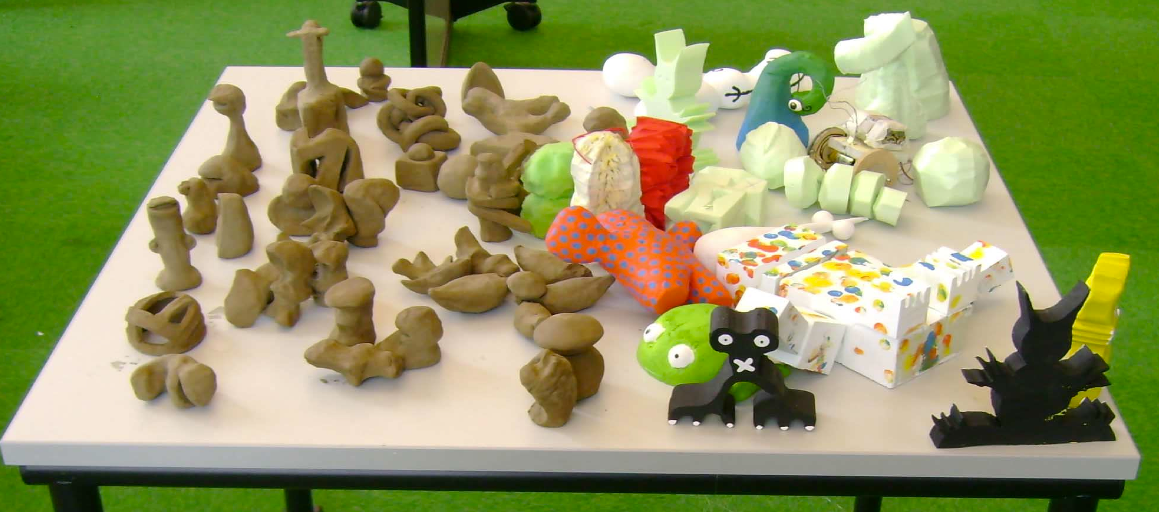
\includegraphics[width=\linewidth]{gfx/vyasModelle}}
	\end{center}
		\caption[Physikalische Modelle. \newline \citep{Vyas:2008}]{Einige physikalische Modelle, erstellt in einem Designstudio.}\label{fig:vyasModelle}
\end{figure}

\begin{quote}
	\textsl{>>One thing that we know is that sketches for experience and interaction desgin will likely differ from conventional sketching since they have to deal with time, phrasing, and feel - all attributes of the overall user experience.<<}
\begin{flushright}\citep{Buxton:2007}\end{flushright}
\end{quote}

Auch wenn sich \emph{Sketches for Experience} von herkömmlichen Skizzen unterscheiden, unterliegen sie trotzdem denselben Eigenschaften.

\medskip Skizzen sollten:
\begin{itemize}
	\item Schnell, reichlich und in kurzer Zeit herstellbar, billig und verwerfbar sein,
	\item Eindeutige Gestik, minimale Detailstufe und angemessenen Grad an Feinheit haben,
	\item und durch Mehrdeutigkeit zum Erforschen und Vorschlagen anregen.
\end{itemize}
\begin{flushright}\citep{Buxton:2007}\end{flushright}

\subsubsection{Low-fidelity Prototypen} \index{Prototyping!Low-fidelity} Skizzen werden auch öfters fälschlicherweise als Prototypen angesehen. Da im nächsten Punkt näher auf Prototypen eingegangen wird, soll an dieser Stelle lediglich auf die Eigenschaften von \emph{Low-fidelity Prototypen}, welche Skizzen am ähnlichsten sind, Bezug genommen und der Unterschied zu Skizzen verdeutlicht werden.

\medskip \emph{Low-fidelity Prototypen} haben wie Skizzen wenig Ähnlichkeit mit fertigen Produkten. Es werden Materialien, wie z.B. Papier oder Karton verwendet, die sich von der gewollten fertigen Version unterscheiden. Sie sind simpel, billig in der Herstellung und leicht zu verändern. \emph{Low-fidelity Prototypen} werden nie mit dem Hintergedanken produziert sie zu behalten und in das Endprodukt zu integrieren \citep{Sharp:2002}.

\medskip Trotz der Ähnlichkeit zu Skizzen, besteht ein feiner Unterschied. Beide beschreiben zwar Designkonzepte, dienen aber unterschiedlichen Zwecken und finden folglich in verschiedenen Stadien des Designprozesses Einsatz. Skizzen werden wie schon erwähnt in den anfänglichen Phasen	der	Ideenfindung verwendet, wobei Prototypen im	Allgemeinen	erst in späteren Phasen eingesetzt werden. Wie \autoref{fig:sagmeisterElaborationReductionFunnels} zeigt, können \emph{Sketching} und \emph{Prototyping} als Trichter im Design Prozess verstanden werden. Am Anfang des Prozesses steht die Ausarbeitung verschiedenster Ideen und Möglichkeiten – am Ende die Reduzierung dieser bzw. die Entscheidungsfindung.
Ebenfalls unterscheidet sich der Aufwand beider Methoden, da Prototypen im Gegensatz zu Skizzen mehr Zeit benötigen bis sie fertig gestellt sind. Sie besitzen somit auch nicht den Wegwerfcharakter einer Skizze. \\
Der Unterschied liegt also nicht in	der	Form der Methoden, sondern eher im Nutzen bzw. in der Bedeutung dieser,	welcher	durch fließende Übergänge beider Methoden in \autoref{fig:buxtonSketch2prototype} anschaulich dargestellt wird \citep{Sagmeister:2008}.

\medskip Per Definition ist eine Skizze ein grobes, ungefähres Design. Es ist lückenhaft, mangelhaft und hat unausgereifte Eigenschaften. Im Gegensatz dazu hilft ein Prototyp Ideen auszuwerten - entweder durch Absprache mit dem Klienten, in der sie ihn ausprobieren, oder durch Usabilitytests. Nicht überraschend, können vorzeitige Usabilityauswertungen von Skizzen bzw. Prototypen, signifikante Probleme aufzeigen, die das Design frühzeitig vernichten - vorallem wenn neue Designs mit konservativeren verglichen werden. Das zieht Folgen für die Entwickler und Forscher mit sich \citep{Greenberg:2008}.
	
\begin{figure}
	\begin{center}
        {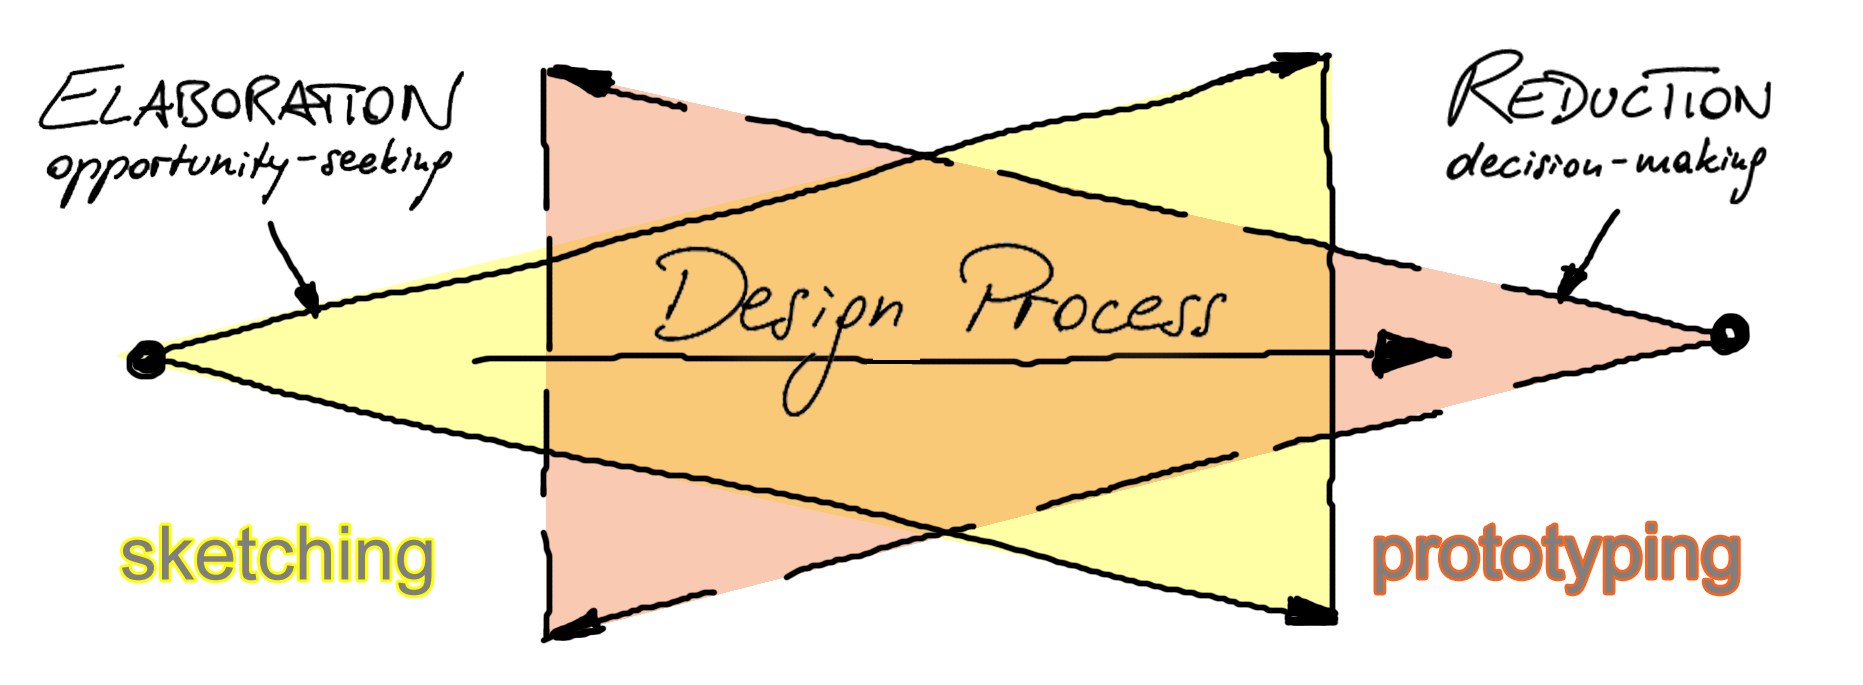
\includegraphics[width=\linewidth]{gfx/sagmeisterElaborationReductionFunnels}}
	\end{center}
		\caption[Skizzen und Prototpyen im Designprozess. \newline \citep{Sagmeister:2008}]{Skizzen und Prototpyen im Designprozess. Die Reduktion, die durch Entscheidungsfindungen bei Prototypen entsteht, wird durch Ausarbeitung von neuen Ideen mit Skizzen ausgeglichen. Dies verdeutlicht die Bedeutungen beider Methoden und deren Einsatzzweck.}\label{fig:sagmeisterElaborationReductionFunnels}
\end{figure}

\begin{figure}
	\begin{center}
        {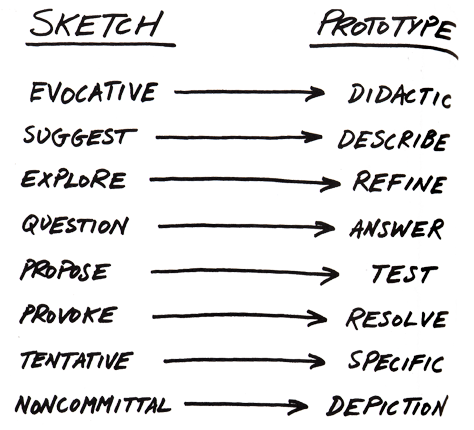
\includegraphics[width=\linewidth]{gfx/buxtonSketch2prototype}}
	\end{center}
		\caption[Übergang von Skizzen zu Prototypen. \newline \citep{Buxton:2007}]{Übergang von Skizzen zu Prototypen. Der Unterschied von Skizzen und Prototypen liegt nicht in der Form der Methoden sondern im Nutzen bzw. in der Bedeutung. Die Pfeile zeigen, dass es sich hierbei um einen fließenden Übergang handelt.}\label{fig:buxtonSketch2prototype}
\end{figure}
\clearpage

\subsubsection{Getting the Right Design vs. Getting the Design Right} \index{Design!getting it right} \label{sssec:rightDesign}
Die Kehrseite frühzeitiger Usability Auswertungen von Skizzen animieren Entwickler jedes Problem in iterativen Schritten zu lösen. Das führt zu >>local hill climbing<<, in dem viel Aufwand betrieben wird um das anfängliche Design richtig hinzubekommen (\emph{Getting the Design Right}) (siehe \hyperref[fig:greenbergBuxtonRightDesign]{Abbildung \ref{fig:greenbergBuxtonRightDesign}a}). Unglücklicherweise blockieren Auswertungen früher Skizzen, Designer oft davon andere, vielleicht bessere Ideen zu entwickeln. \citep{Greenberg:2008}

\medskip Eine Skizze bildet typischerweise nur eines der möglichen Designs und Variationen zum Abwägen ab. Frühes Design benötigt jedoch viele Ideenskizzen, einen Vergleich vieler konkurrierender Ideen und eine Auswahl des aussichtsvollsten Designs (siehe \hyperref[fig:greenbergBuxtonDesignRight]{Abbildung \ref{fig:greenbergBuxtonDesignRight}}). Die aussichtsvolle Idee wird dann weiter abgestimmt und entwickelt, bis man sie als Prototyp verwenden kann. In anderen Worten: Skizzieren dreht sich um das Finden des richtigen Designs (\emph{Getting the Right Design}) \citep{Tohidi:2006, Buxton:2007, Greenberg:2008}. 

\begin{figure}
	\myfloatalign
	\subfloat[Getting the Right Design.]
	{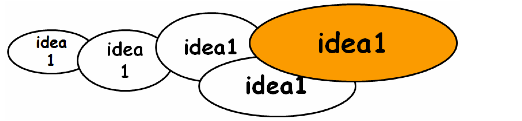
\includegraphics[width=\linewidth]{gfx/greenbergBuxtonDesignRight}} \\
	\subfloat[Getting the Design Right.]
	{\label{fig:greenbergBuxtonDesignRight}%
	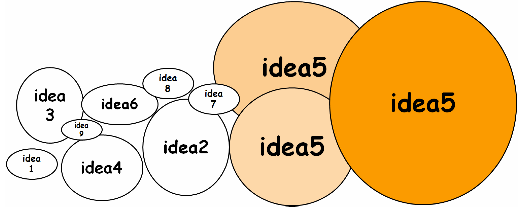
\includegraphics[width=\linewidth]{gfx/greenbergBuxtonRightDesign}} \\
	\caption[Getting the Right Design vs. Getting the Design Right. \newline \citep{Greenberg:2008}]{Getting the Right Design vs. Getting the Design Right. Die richtige Herangehensweise ist das Erstellen von Skizzen, danach das iterative Design, gefolgt von Auswertungen.}\label{fig:greenbergBuxtonRightDesign}
\end{figure}

\subsection{Prototyping} \index{Prototyping}
Der abschließende und wichtigste Schritt bevor ein Produkt oder Service engeführt, oder idealerweise mit Benutzern getestet wird, ist die Erstellung eines Prototyps - oder besser mehrerer Prototypen.

\begin{quote}
	\textsl{>>Prototyping is where, finaly, all pieces of the design come together in a holistic unit.<<}
\begin{flushright}\citep{Saffer:2007}\end{flushright}
\end{quote}

Viele Auftraggeber haben Schwierigkeiten ein Design zu verstehen, bevor sie nicht einen Prototypen gesehen und benutzt haben. Prototypen sind ein Kommunikationswerkzeug. Sie übermitteln die Botschaft >>So könnte das Ganze aussehen und funktionieren<<.

\medskip Industrial Designer z.B. erstellen in dieser Phase ein glaubwürdiges Modell eines Produktgehäuses, einschließlich Knöpfe, Drehschalter oder anderer Bauteile, welches so real aussieht, dass es sogar die Auftraggeber täuschen kann. Zusätzlich werden oft Screen Designs, Animationen oder interaktive Demonstrationen erstellt, um Benutzern zu zeigen, wie das Produkt reagieren soll \citep{Vertelney:1990}.

\medskip Welche Form aber nun Prototypen im Allgemeinen annehmen, hängt von den Mitteln ab, die Designern zu Verfügung stehen bzw. von der Art des Produkts um das es sich handelt. Ein Designer mit den richtigen Ressourcen kann \emph{high-fidelity Prototypen} erstellen, welche so aussehen und reagieren als wären sie das fertige Produkt.

Der Zweck von Prototypen ist aber das Erforschen der Eigenschaften des Endprodukts. Ein Prototyp ist vielleicht effizient und ausdruckslos und ein anderer ist wiederum skurril und zugänglich. Der eine ist Menü-basiert und der andere benutzt direkte Manipulationen. Designer benutzen Prototypen um herauszufinden, welche Funktionen oder Eigenschaften funktionieren, und zwar für sich selbst, die Auftraggeber und die Benutzer \citep{Saffer:2007}. Da Designer nicht unfehlbar sind und somit das erste Design nicht perfekt sein wird, werden die Erkenntnisse, welche aus diesen sog. \emph{>>formative Evaluations<<} gewonnen werden, zur Erstellung verbesserter Prototypen benutzt. Dieser iterative Prozess aus Verbesserungen läuft so lange bis klarer weise keine Verbesserungen mehr nötig sind. Oder mit anderen Worten: 

\begin{quote}
	\textsl{>>This is exactly how iterative prototyping works: you start somewhere, evaluate it to see how to make it better, change it to make it better and then keep on doing this until it can't get any better.<<}
\begin{flushright}\citep{Dix:2004}\end{flushright}
\end{quote}

Eine Gefahr, die Prototyping mit sich bringen kann, ist die Wahl eines falschen Anfangsdesigns. Wenn man mit einem schlechten Design-Konzept beginnt Prototypen zu erstellen, kann es sein, dass man am Ende nur eine >>verschönerte<< Version der schlechten Idee bekommt (vgl. \ref{sssec:rightDesign} \nameref{sssec:rightDesign}).\\ Die Vorraussetzungen um Prototyping Methoden richtig einsetzen zu können sind also:

\begin{enumerate}
	\item Ein Verständnis über die Elemente die neu designed gehören und wie man sie verbessern kann, und
	\item Ein gutes Anfangsdesign als Startprodukt.
\end{enumerate}
\begin{flushright}\citep{Dix:2004}\end{flushright}

Gute Designer schaffen es vielleicht auch durch Erfahrung und Urteilungsvermögen ein passendes Anfangsdesign zu finden, jedoch wird auch ihnen dies durch die Komplexität der Probleme, gerade in Interaction Design, erschwert. Das Ausarbeiten von Skizzen und Modellen, um Probleme aus verschiedenen Blickwinkeln zu beleuchten ist deswegen gerade vor dem Erstellen von Prototypen essenziell.
Die meisten Designer arbeiten mit drei Arten von Prototypen: Digitalen Prototypen, physikalischen Prototypen und Prototypen aus Papier. Es soll nun kurz näher auf diese eingegangen und im Besonderen \emph{Paper Prototyping} diskutiert werden. 

\subsubsection{Digitale Prototypen} \index{Prototyping!Digital}
Digitale Prototypen (siehe \autoref{fig:safferDigitalPrototype}) können verschiedenste Formen annehmen, von statischen Bildern bis hin zu komplexen 3D Umgebungen. Sie können in ihrer Funktionalität sehr eingeschränkt sein – z.B. indem sich Benutzer durch eine Reihe an Bildern >>durchklicken<< - oder im hohen Grade funktionell, so dass User in der Lage sind mit dem System zu arbeiten als wäre es das Endprodukt. Entscheidet man sich für die komplexere Variante, sollten reichhaltig Funktionen vorhanden sein, um das problemlose Interagieren des Users gewährleisten zu können. Es ist schwer für Benutzer sich z.B. ein Werkzeug um Rechtecke zu zeichnen vorzustellen, ohne es dabei wirklich benutzen zu können. Die Gefahr dabei ist jedoch, dass Benutzer und Auftraggeber denken könnten, dass der Prototyp bereits das finale Produkt ist. Fügt man einmal ein visuelles Design hinzu, richtet man seine Aufmerksamkeit diesem anstatt auf die Funktionalität \citep{Saffer:2007}.\\
Seit den 80er Jahren gibt es für beide Formen digitaler Prototypen eine Vielfalt an Programmen zur Erstellung dieser. Seien es Programme wie \emph{MacDraw}, \emph{Protoscreens}, oder \emph{Prototyper} damals, oder Tools wie \emph{Photoshop}, \emph{Shockwave} oder \emph{Visual Basic} heutzutage; sie alle verfügen über die Funktionalität, Prototypen (mit ihren beschränkten Grad an Nutzen) zu erstellen \citep{Miller-Jacobs:1991}. \\
Ein Vorteil der daraus entsteht, ist dass digitale Prototypen leicht veröffentlicht werden können. Designer können sie einfach aufs Web stellen oder auf Disks verbreiten, um Benutzern die Möglichkeit zu bieten, die Prototypen egal wo sie sind auszuprobieren. 

\begin{figure}
	\begin{center}
        {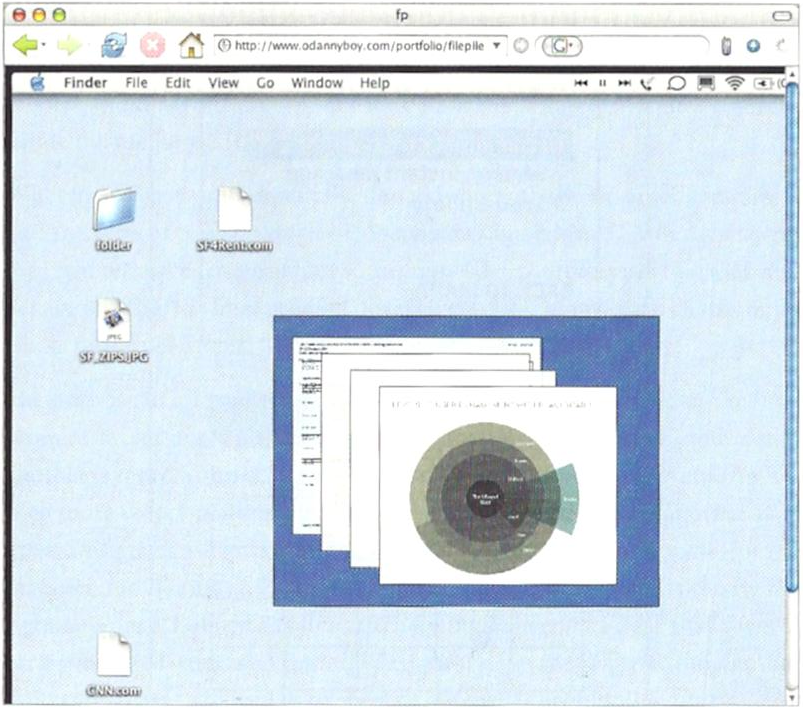
\includegraphics[width=\linewidth]{gfx/safferDigitalPrototype}}
	\end{center}
		\caption[Digitale Prototypen. \newline \citep{Saffer:2007}]{Digitale Prototypen können Formen in verschiedener Detailstufen annehmen und leicht über das Internet verbreitet werden.}\label{fig:safferDigitalPrototype}
\end{figure}

\subsubsection{Physikalische Prototypen} \index{Prototyping!Physikalisch}
Physikalische Prototypen (siehe \autoref{fig:safferPhysicalPrototype}) können simple Teile eines Designs (wie zum Beispiel einzelne Schalter oder Wahltasten) bis hin zu kompletten physikalischen Umgebungen schaffen. Wie aber auch bei anderen Prototypen kann sich dabei die Funktionalität und Beschaffenheit unterscheiden. Ein Gerät beispielsweise kann aus exakt denselben Materialien wie das Endprodukt erstellt werden (z.B. Plastik oder Metall), oder durch Materialien wie Holz oder Ton angeglichen werden. 

\begin{figure}
	\begin{center}
        {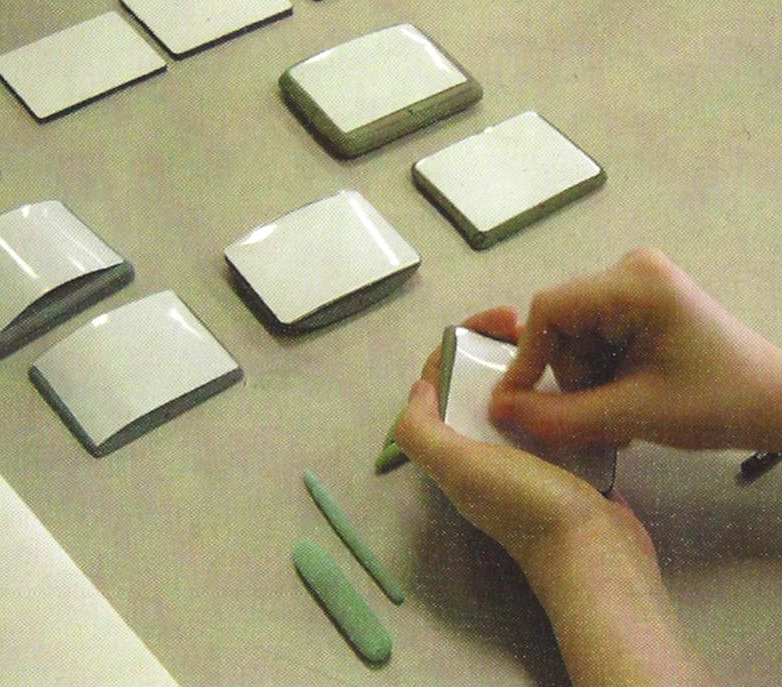
\includegraphics[width=.8\linewidth]{gfx/safferPhysicalPrototype}}
	\end{center}
		\caption[Physikalische Prototypen. \newline \citep{Saffer:2007}]{Physikalische Prototypen können so klein wie ein Schalter sein, oder so groß wie ein ganzer Raum.}\label{fig:safferPhysicalPrototype}
\end{figure}

\subsubsection{Papier Prototypen} \index{Prototyping!Papier}
Papier Prototypen sind meistens die schnellste Art um die Funktionalität eines Produkts oder Services zu demonstrieren. Vor allem im Interaction Design kann ein Designer auf Papier leicht einen gesamten Systemdurchlauf erstellen, wobei jedes Blatt Papier einen ‚Moment’ des Designs repräsentiert. Diese Momente könnten eine Webseite, ein Screenshot oder Teil eines Services sein. Zuseher können so Schritt für Schritt den Prototyp durchlaufen indem sie sich in einer gewissen Reihenfolge zwischen den Seiten bewegen.
Wie diese Bewegung abläuft, kann auf mehrere Arten erfolgen. Dan Saffer z.B. schlägt vor die Seiten zu nummerieren, und dem User klare Instruktionen zu geben wie er vorzugehen hat („Wenn Sie diesen Button drücken, gehen Sie auf Seite 9“). Während des Testens können bei diesem Verfahren Beteiligte, also Benutzer und Designer, Kommentare und Notizen direkt auf dem Prototyp schreiben \citep{Saffer:2007}.\\
Carolyn Snyder hingegen vertritt eine andere Auffassung von \emph{Paper Prototyping}: 

\begin{quote}
	\textsl{>>Paper prototyping is a variation of usability testing where representative users perform realistic tasks by interacting with a paper version of the interface that is manipulated by a person "playing computer", who doesn't explain how the interface is intended to work.<<}
\begin{flushright}\citep{Snyder:2003}\end{flushright}
\end{quote}

Laut ihr hat mindestens eine Person neben dem User zu sitzen und agiert (vollkommen still) als Computer und übernimmt dessen Aufgaben. Kommentare und Notizen machen andere Personen, die ebenfalls still als Beobachter im Raum sitzen. Zusätzlich kann noch ein Moderator hinzu gezogen werden, welcher dem User das Umfeld erklärt bzw. ihm Aufgabenstellungen erteilt.

\medskip Im Allgemeinen signalisieren Papier Prototypen, egal nach welcher Methode erstellt, den Benutzern, dass es sich hierbei noch nicht um das Endprodukt handelt und gewähren ihnen somit unterbewusst mehr Freiheiten, Eigenschaften und Funktionsweisen zu kommentieren. Snyder fasst weiters folgende Vorteile zusammen:

\medskip Papier Prototypen:
\begin{itemize}
	\item Liefern substanzielles User Feedback in einem frühem Stadium des Entwicklungsprozesses (bevor Bemühungen in die Implementierung gesteckt wurden),
	\item Fördern schnelle iterative Entwicklung, durch Experimente mit mehreren Ideen, anstatt nur mit einer,
	\item Erleichtern die Kommunikation innerhalb des Entwicklungsteams sowie zwischen dem Team und den Benutzern,
	\item Erfordern keine technischen Fähigkeiten, womit eine multidisziplinäre Mannschaft zusammenarbeiten kann, und
	\item Regen Kreativität im Produktentwicklungsprozess an.
\end{itemize}
\begin{flushright}\citep{Snyder:2003}\end{flushright}
	
Paper Prototyping folgt somit dem >>Maximum Feedback for Minimum Effort<< - Prinzip. Wie sieht aber nun ein Papier Prototyp aus und wie wird er erstellt?

\medskip Materialien wie einfaches weißes Papier, unlinierte Karteikarten, Marker, Stifte, Scheren, durchsichtiges entfernbares Klebeband, transparente Folien, Permanentmarker usw. dienen als Werkzeuge in Paper Prototyping.\\
Durch sie werden anfangs Hintergründe bzw.  Hintergrundsmasken\index{Hintergrundsmasken} kreiert. Diese können z.B. gezeichnete Repräsentationen eines Browserfensters sein, wenn der Browser mit seinen herkömmlichen Funktionen über den Testverlauf hinweg unverändert bleibt, oder andere statische Gegebenheiten. Ein Hintergrund ist zwar nicht immer notwendig, zeigt dem Benutzer jedoch, dass er es mit einer Repräsentation eines Computerbildschirms oder anderen elektronischen Gerät zu tun hat und sich somit auf diese konzentrieren soll. Es kann manchmal auch helfen - besonders bei kleinen Geräten (z.B. bei PDAs oder Handys) – durch Masken den nutzbaren Platz zu begrenzen, da gerade hier oft jeder Pixel zählt. \autoref{fig:snyderMasks} zeigt dazu ein Beispiel. \\
Nachdem die Hintergründe bzw. Masken\index{Masken|see{Hintergrundsmasken}} erstellt wurden, ist es nötig alle Interface Widges, wie \emph{buttons}, \emph{checkboxes}, \emph{dialog boxes}, \emph{text fields}, \emph{lists}, \emph{cursors} etc. zu erstellen. Interface Widges helfen später im User Testing die Interaktivität zu simulieren \citep{Snyder:2003}.

\begin{figure}
	\begin{center}
        {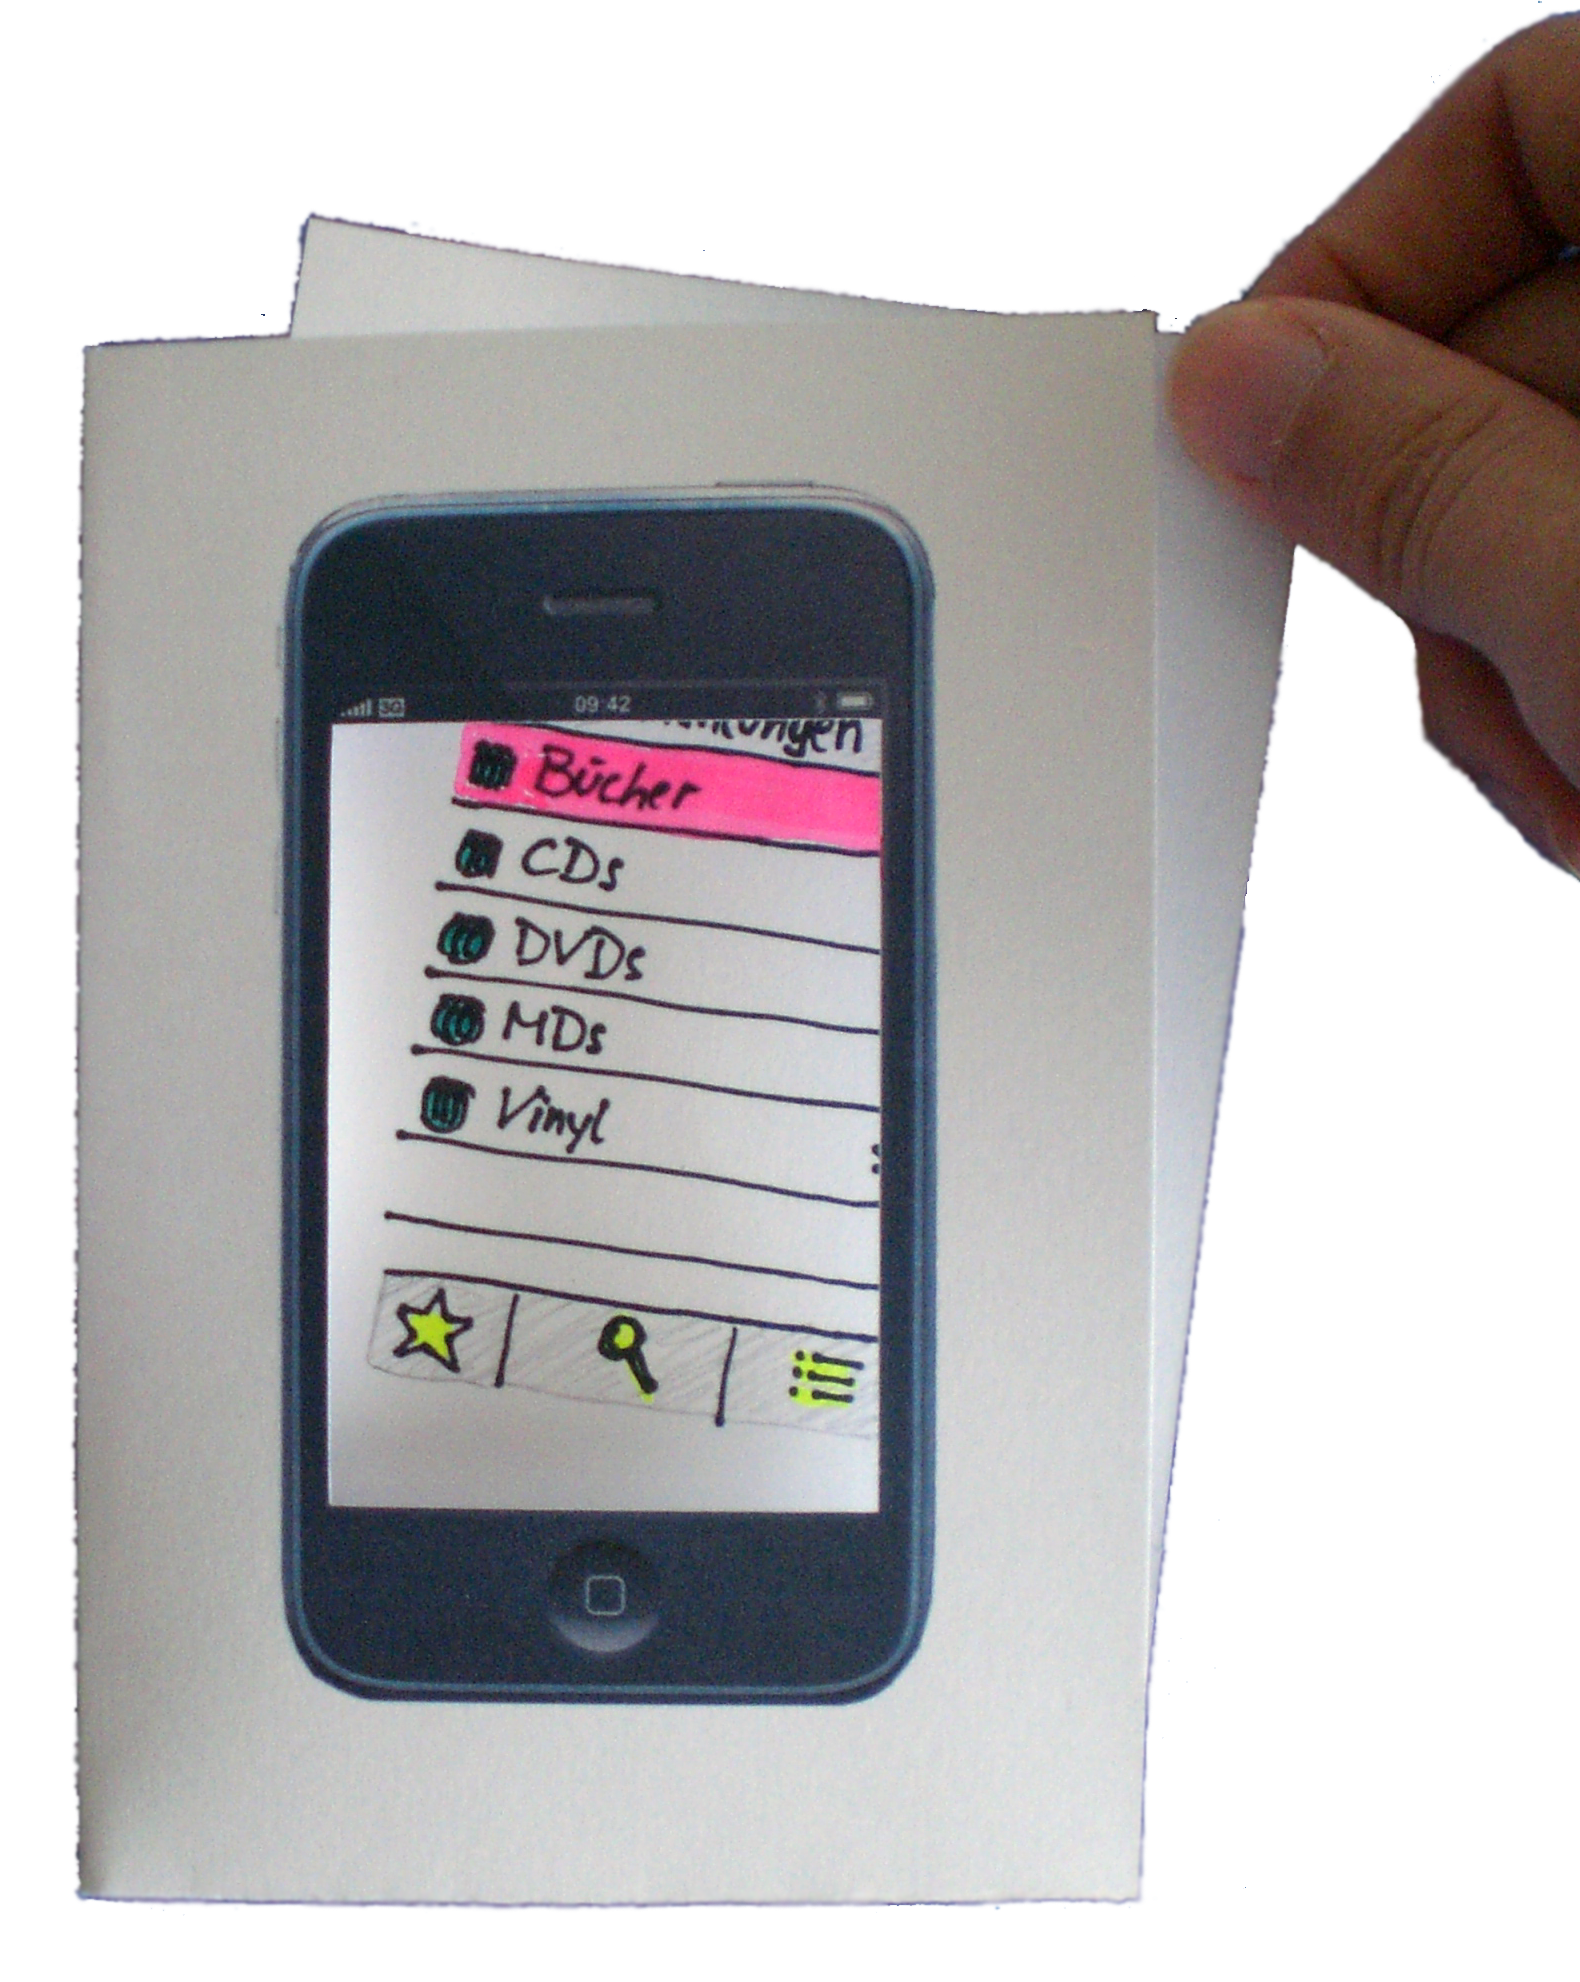
\includegraphics[width=.7\linewidth]{gfx/snyderMasks}}
	\end{center}
		\caption[Hintergrundmasken \newline \citep{Snyder:2003}]{Hintergrundmasken werden im ersten Schritt von Paper Prototyping erstellt. Besonders bei kleinen Geräten kann es helfen, den nutzbaren Bereich einzugrenzen, da hier meist jeder Pixel zählt.}\label{fig:snyderMasks}
\end{figure}

\medskip Sie sollten deswegen so gut wie möglich vorbereitet werden, um lange Wartezeiten im Testing zu vermeiden. Im Allgemeinen ist es natürlich auch erlaubt Screenshots von Elementen (inklusive Hintergrund) zu machen, jedoch muss man sich dabei immer fragen wie viel man vielleicht nachträglich ändern will. Meistens ist es schneller, Elemente selbst zu zeichnen. \autoref{fig:snyderPaperPrototype} zeigt Vorbereitungselemente aus den verschiedensten Materialien und deren möglichen Einsatzzweck \citep{Snyder:2003}.

\begin{figure}
	\myfloatalign
	\subfloat[Papierelemente]
	{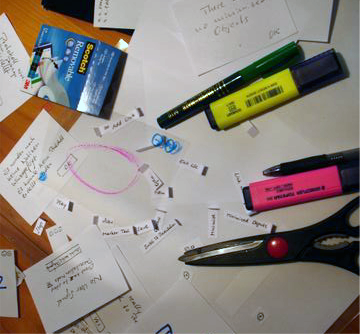
\includegraphics[width=.48\linewidth]{gfx/snyderPaperElements}} \quad
	\subfloat[Papier Prototyp]
	{\label{fig:snyderPaperElements}%
	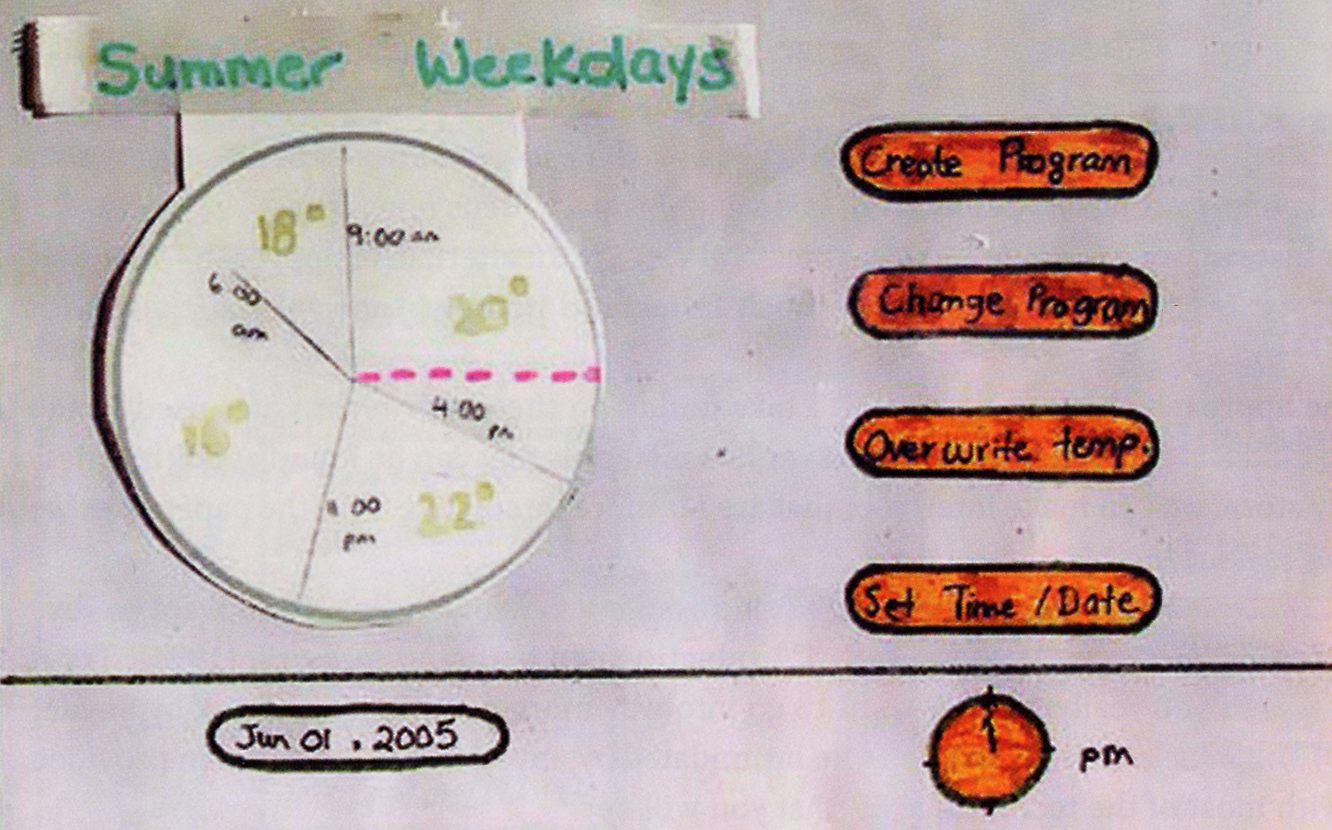
\includegraphics[width=.48\linewidth]{gfx/snyderPaperPrototype}} \\
	\caption[Paper Prototyping \newline \citep{Sagmeister:2008}]{Papierelemente (a) für Interface Widges können durch einfache Materialien wie Papier und Stifte erstellt werden. Sie sollten vor dem User Testing vorbereitet werden, um lange Wartezeiten zu vermeiden. Ein Papier Prototyp, wie in (b), imitiert zwar nur das Enprodukt, bietet dem User aber die volle Interaktivität. Der Benutzer interagiert dabei direkt mit dem Prototypen als wäre es ein Touch Screen.}\label{fig:snyderPaperPrototype}
\end{figure}

\medskip Nachdem ein Prototyp fertig gestellt wurde, sollte er logischerweise auch Einsatz finden. Das richtige Publikum dafür sind die User, die das Endprodukt benutzen werden. Man nennt diesen Prozess auch User Testing, der im folgenden Punkt beschrieben wird.

\subsection{(User) Testing} \index{Testing} \index{User Testing|see{Testing}}
Der oft verwendete Begriff User Testing ist eigentlich eine Fehlbezeichnung. Getestet werden natürlich nicht die User sondern das Produkt bzw. das Service. 
Das Testen mit potentiellen Benutzern hilft falsche Annahmen, die in der Vorbereitung bzw. Erstellung des Designs gemacht wurden, zu korrigieren. Am besten werden diese durch Beobachtungen und Rücksprache mit den Testpersonen aufgedeckt. Dabei ist es oft am besten, wenn Designer anderen Teammitgliedern oder \emph{Usability Spezialisten} gestatten die Tests zu leiten, um selbst eine Beobachterrolle einzunehmen. Designer neigen meist dazu ihr Gegenüber zu belehren (>>Schau doch mal zu den Button rechts oben<<), weil sie ihr Design besser kennen. Es sollte zusätzlich vermieden werden, dass sich Designer als solche zu erkennen geben, da Testpersonen oft ihr Feedback danach richten bzw. gegebenenfalls ihre Kritik abschwächen. Auch wenn für Designer nichts demütigender ist, als anzusehen wie Testpersonen durch ihr Design stolpern, müssen sie diese Bürde auf sich nehmen, die Testdurchläufe ernst nehmen und nach Verhaltensmustern Ausschau halten.  Diese bewegen sie dann dazu, Prototypen zu ändern und sie erneut zu testen. Erfahrene Designer wissen eins mit Sicherheit: Das erste Design ist es selten das richtige. \\
Testings werden am besten direkt im geplanten Umfeld der Endnutzer durchgeführt, es sei denn ein handelt sich um ein Service, dass eine bestimmte Prototypumgebung erfordert. Digitale und physikalische Prototypen sollten somit auf ihren geplanten Computern und Umfeldern Anwendung finden (vgl. \autoref{fig:safferUserTesting}). Papier Prototypen erfordern eine bestimmte Prototyp-umgebung, die es erlaubt die Testings auch in Testlaboratorien o.ä. durchzuführen. Testlaboratorien haben den Vorteil, dass Designer viele Tests an einem einzigen Tag durchführen können, ohne dabei den Ort wechseln zu müssen \citep{Saffer:2007}.

\medskip Je nach Qualität bzw. Aufwand der für einen Prototypen betrieben wurde, variiert auch der Ablauf eines User Testings. Oft reicht es, wie z.B. bei \emph{high fidelity} Digitalprototypen, dem User lediglich eine Aufgabe zu stellen und ihn dann sich selbst zu überlassen um ihn zu beobachten. Manchmal benötigt man auch einen Moderator, der den User durch den Testablauf leitet. Bei \emph{low fidelity} Prototypen jedoch, zu denen meist Papierprototypen zählen, muss mehr Aufwand betrieben werden. Wie schon im vorigen Punkt erwähnt, ist es notwendig jemanden den Part des Computers bzw. Gerätes übernehmen zu lassen. Bei Paper Prototyping sitzt diese Person meist neben oder gegenüber der Testperson und übernimmt stillschweigend alle interaktiven Tätigkeiten.

\medskip Dieses Prinzip ist aber nicht nur eine Eigenheit von Papierprototypen. Eine der ersten Anwendungen fand sich schon 1971 mit dem Testen eines elektronischen Flugticket Schalters am Chicago O’Hare Airport \citep{Erdmann:1971}. Da es von echten Kunden, mit echtem Geld zur Anschaffung echter Tickets für damals aktuelle Flüge verwendet wurde, musste es nicht nur von der \emph{user-interaction}-Perspektive, sondern auch von der organisatorischen und finanziellen Seite her arbeiten. Doch da das System noch nicht fertig gestellt war und man es trotzdem einem Test unterziehen wollte, musste eine Person im Hintergrund alle Tätigkeiten, wie am normalen Ticketschalter, managen. Auch wenn es aus Sicht des Kundenservices teuer und ineffizient schien, brachte es wichtige Informationen über das Desgin, die \emph{Usability} und die Akzeptanz mit sich \citep{Buxton:2007}.

\begin{figure}
	\begin{center}
        {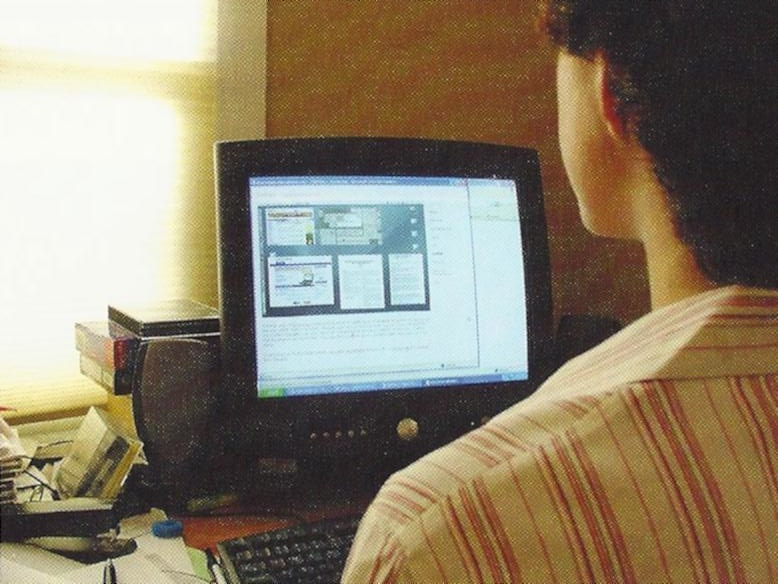
\includegraphics[width=\linewidth]{gfx/safferUserTesting}}
	\end{center}
		\caption[(User) Testing \newline \citep{Saffer:2007}]{Testings werden am besten im geplanten Umfeld der Endnutzer durchgeführt. Ein digitaler Prototyp sollte z.B. beim Benutzer zu Hause getestet werden.}\label{fig:safferUserTesting}
\end{figure}

\begin{figure}
	\begin{center}
        {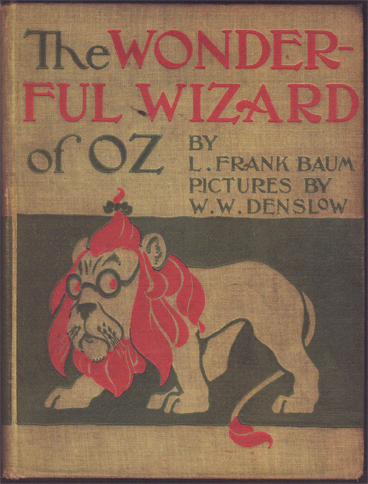
\includegraphics[width=\linewidth]{gfx/buxtonWizardOz}}
	\end{center}
		\caption[Wizard of Oz \newline \citep{Buxton:2007}]{Das Cover der Erstedition des Buches, das einen unerwarteten Einfluss auf das Thema Interaction Design zur Folge hatte. Die Wizard of Oz Technik beschreibt eine Interaktion zwischen Mensch und Maschine in der eine Person die Reaktionen eines Systems erzeugt.}\label{fig:buxtonWizardOz}
\end{figure}

\medskip Diese Art des Testens nennt man auch \emph{Wizard of Oz Technique}\index{Wizard of Oz Technique}, die ihren Ursprung in der Kindergeschichte \emph{The Wonderful Wizard of Oz} von L. Frank Baum findet. (siehe \autoref{fig:buxtonWizardOz}) \\ Sie handelt von einem kleinen Mädchen Dorothy, welches zusammen mit ihrem Hund Toto von einem Wirbelsturm von ihrer Farm in Kansas in das Land der Munchkins getragen wird. Verzweifelt, mit dem Wunsch wieder nach Hause zu kommen, traf sie auf die Gute Hexe des Nordens, die der gelandeten Dorothy riet, in die Smaragdstadt zu gehen und dort den Zauberer von Oz um Hilfe zu bitten. Mit neu gefunden Freunden zog Dorothy los und fand tatsächlich den Zauberer, der sich jedem in einer anderen Gestalt zeigte. Er versicherte zu helfen, unter der Bedingung, dass einer die Böse Hexe des Westens tötet. Nach einigen Abenteuern schafften sie dies auch und kehrten zurück zum Zauberer um das Versprechen, das er ihnen gab einzulösen. Nach anfänglichem Zögern seitens des Zauberers von Oz, sich zu zeigen, brachten sie ihn schlussendlich dazu und mussten feststellen, dass er gar kein großer Zauberer war, sondern nur ein alter Mann, den durch seine Ankunft mit einem Heißluftballon jeder als Magier ansah. \citep{Baum:2008}

\medskip Dorothy und ihr Hund Toto fanden natürlich einen anderen Weg nach Hause, die Geschichte zeigte uns aber, dass hinter dem großen \emph{Wizard of Oz} ein schüchterner alter Mann steckte, der mit seinem Trick so überzeugend war, dass er alle glauben ließ er sei jemand, der er gar nicht war. Und das ist auch die Quintessenz: 

\begin{quote}
	\textsl{>>To her the Wizard was real, and therefore so were all her experiences.<<}
\begin{flushright}\citep{Buxton:2007}\end{flushright}
\end{quote}

Folgt man also dem Beispiel des Zauberers, kann man im User Testing Systeme >>herbei beschwören<<, die den Benutzern reale wirkungsvolle Erfahrungen bieten, bevor das richtige System im eigentlichen Sinne existiert. Die wichtigsten Punkte, die man dabei beachten sollte sind folgende:

\medskip Eigenschaften von Testsystemen:\index{Testsysteme}
\begin{itemize}
	\item Es ist das Detailreichtum der Erfahrung und nicht die des Prototyps, Skizze oder Technologie, die wichtig ist, im Sinne der Ideenfindung und des Anfangsdesigns.
	\item Man kann alles verwenden, um diese Erfahrungen >>zu beschwören<<.
	\item Umso früher damit begonnen wird, desto wertvoller sind sie.
	\item Es ist einfacher, billiger, schneller und zuverlässiger einen alten Mann, ein Mikrofon und Lautsprecher zu finden als einen richtigen Zauberer. Dies gilt auch für die meisten Systeme:  Fake it before you build it.
\end{itemize}
\begin{flushright}\citep{Buxton:2007}\end{flushright}
	
Die Zielsetzung ist also nicht, das tatsächliche System zu bilden, sondern etwas nach zu ahmen, das Benutzer wirklich erfahren können. Das ermöglicht Design Konzepte in ihrer Tätigkeit zu erforschen und sie viel früher im Prozess zu erfahren als sonst möglich. Solch ein System sollte preiswert, schnell zu verwirklichen und verwerfbar sein und nur soviel Detailreichtum wie nötig besitzen, um seinen Zweck zu erfüllen. Es sollte somit alle Eigenschaften aufweisen, die auch Skizzen kennzeichnet, jedoch einer Regel unbedingt unterliegen: 

\begin{quote}
	\textsl{>>Generally the last thing that you should do when beginning to design an interactive system is write code.<<}
\begin{flushright}\citep{Buxton:2007}\end{flushright}
\end{quote}	

Mit den richtigen Testsystemen und klaren Aufgabenstellungen ist es für die Designer einfacher bestimmte Verhaltensmuster aus den Benutzererfahrungen zu erkennen. Oft werden zusätzlich im Laufe des Testings zu den vordefinierten Aufgaben, die Zeit und die Fehlerquote gemessen bzw. der Weg, wie ein User ein Problem löst, aufgezeichnet. Dies soll messbare Qualitätsmerkmale über das Design liefern und bei den abschließenden Rücksprachen mit den Benutzern Orientierungshilfe bieten.
Gewöhnlich werden 5-12 Testpersonen in ein Testing miteinbezogen. \citep{Dumas:1999} Meist sind es aber weniger, da man sich an einen fixen Projektzeitplan halten muss. Deswegen werden oft auch nur \emph{Quick and Dirty} – Tests mit 1-2 Usern durchgeführt, um schnelles Feedback zu einer Designidee zu bekommen \citep{Sharp:2002}.

\medskip Skizzieren, das Erstellen von Prototypen und Testen sind wichtige Methoden, um Ideen zu sammeln, sie zu einem Design zusammenzutragen und durch Erfahrungen zu verbessern bevor das endgültige Produkt erstellt wird. Viele Designer arbeiten mit ihnen effektiv und uneingeschränkt, jedoch ist es manchmal hilfreich zu wissen, von wem und wie genau ein Produkt verwendet werden soll. Dies wird nun abschließend im letzten Punkt erläutert.

\subsection{Personas \& Szenarien} \index{Personas} \index{Szenarien}

Der Begriff Personas umfasst eine Sammlung an typischen Personen, die mit einem Produkt oder Service zu tun haben. Sie zeigen Designern, dass sie für bestimmte Personen mit bestimmten Eigenschaften und Vorlieben designen und nicht schlicht für >>die Benutzer<<. 
Designer erfinden aus diesem Grund verschiedene Personas mit Hilfe von Beobachtungen und Unterhaltungen mit Usern. Zitate von diesen sind z.B. sehr nützlich, um Personas zu beschreiben (>>Ich fliege mindestens einmal pro Woche<<), oder um einfache Überschriften (>>Der häufige Passagier<<) zu finden. Personas fassen also Personen zusammen, die ähnliche Ziele, Beweggründe und Verhalten teilen. Ein Persona Dokument sollte diese Eigenschaften klar aufzeigen, um eine Persona von einer anderen unterscheiden zu können (siehe \autoref{fig:safferPersona}).

\begin{figure}
	\begin{center}
        {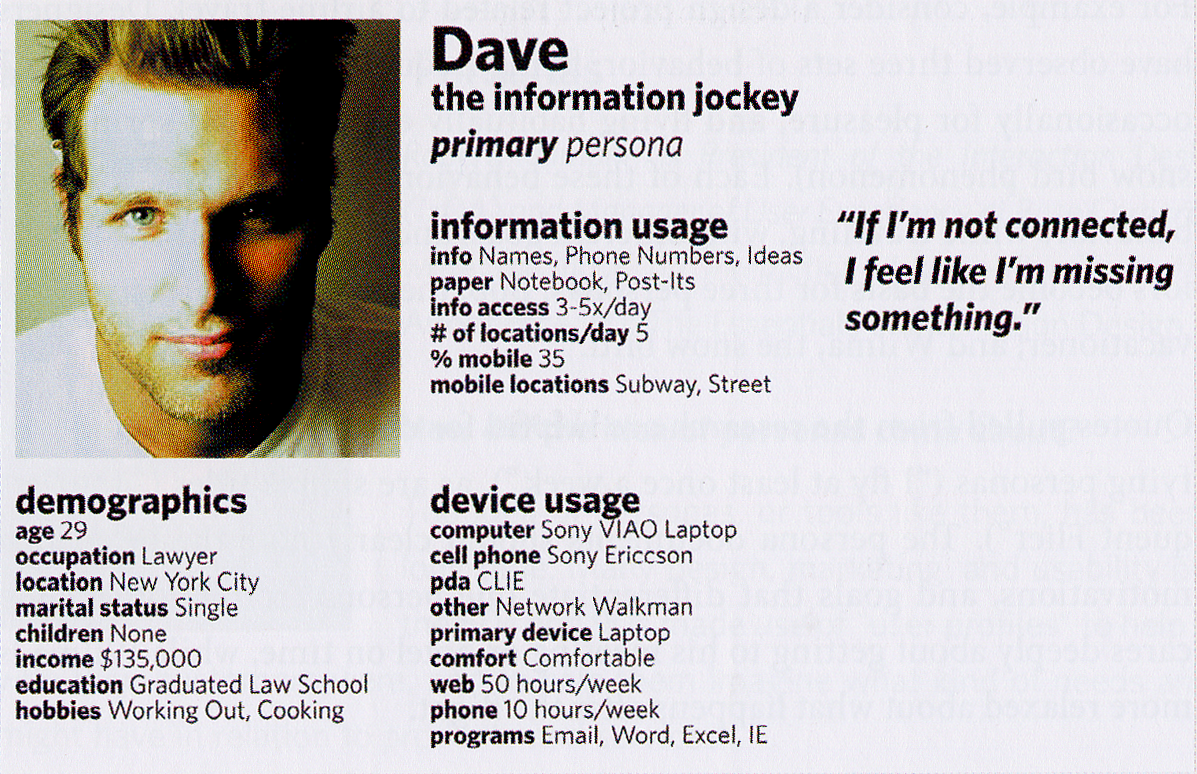
\includegraphics[width=\linewidth]{gfx/safferPersona}}
	\end{center}
		\caption[Persona \newline \citep{Saffer:2007}]{Personas verwandeln >>die Benutzer<< in identifizierbare menschliche Wesen.}\label{fig:safferPersona}
\end{figure}

\medskip Im Allgemeinen sollte man die Anzahl an Personas gering halten – am besten zwischen eins und sieben. Nach ca. sieben Personas fällt es einem schwer, sich an alle zu erinnern bzw. sie unterscheiden zu können. (vgl. \ref{ssec:GuidingPrinciples} \nameref{ssec:GuidingPrinciples}) Vor allem wird es mit zunehmender Anzahl immer schwieriger ein Design zu finden, welches allen Ansprüchen genügt. Man muss sich deswegen stets darum bemühen sich an das Kernverhalten zu richten, und nicht an alle verschiedenen Facetten.

\medskip Nachdem eine Sammlung an Personas zusammengestellt wurde, sollte man ein Foto für jede finden. Bilder helfen mehr als alles andere, eine persönliche Note hinzuzufügen und um sich leichter an diese zu erinnern. So lange Personas nicht veröffentlicht werden, können Fotos auch von Services wie z.B. \emph{Yahoo Personals} oder anderen Internetseiten verwendet werden. Personas an sich sind schlicht unbrauchbar wenn sie nicht zusammen mit Szenarien eingesetzt werden. In Szenarien können sie benutzt werden um Systemeigenschaften auf Nutzen und Eignung zu testen. 
Während viele Designer Personas nützlich finden, lehnen sie mache ganzheitlich ab. Diese Designer sehen Personas als eine Art künstliche Blockade zwischen dem Produkt und dessen Benutzer. Personas können jedoch, wenn sie auf Forschungen basieren und die richtigen Charakteristiken (Verhalten, Motivationen und Ziele) zeigen als wertvolles Tool dienen. Ob man Personas nun verwenden will, hängt schlussendlich vom Designer und der Größe des Projektes ab. \citep{Saffer:2007}

\medskip \emph{Szenarien} hingegen bieten einen schnellen und effektiven Weg um sich Design Konzepte vorzustellen. Man kann sie sich als Prototypen, welche lediglich aus Wörtern bestehen, vorstellen, da sie simple Geschichten bilden, welche fertig gestellte Produkte beschreiben. Die zentralen Darsteller dieser Geschichten sind Personas, die durch sie einen Kontext erhalten und zum Leben erwachen. Das Durchlaufen eines Szenarios mit verschiedenen Personas eignet sich somit perfekt zur Darstellung, Analyse und Planung der Auswirkungen eines Systems auf das Verhalten der User. Man betrachte folgendes Beispiel eines Szenarios:

\begin{quote}
	\textsl{>>Sarah logs onto her BigGrocery account. She sees her order from last week and decides to use it again for this week's order. She removes a few items by dragging them off her BigGroceryList. Her total cost adjusts appropriately. She has all the groceries she wants now, so she clicks the Deliver button. Her saved credit card account is charged, and her confirmation page tells her to expect the groceries in about an hour.<<}
	 \begin{flushright} \citep{Saffer:2007} \end{flushright}
\end{quote}

Dieses Szenario nahm nur ein paar Minuten in Anspruch um es zu schreiben, aber es würde Stunden benötigen um ein Storyboard\index{Storyboards}\footnote{Storyboards haben ihren Ursprung in der Filmindustrie. Sie bestehen aus Bildern (potentiellen Screenshots) und dazugehörigen Beschreibungen. Zusatzinformationen über den Ablauf werden durch Bildübergänge  erreicht. \emph{>>Storyboarding is a way to look at the film without spending a lot of money \ldots It’s not the ultimate film, but it represents a first chance to look at it<<} -- Production Illustrator Marty Kline \citep{Braa:1989}}  zu erstellen, Tage um es realistisch darzustellen, und Wochen um einen Prototypen anzufertigen. Mit der Hilfe von Szenarien sind Designer in der Lage mit Wörtern zu skizzieren. \citep{Saffer:2007} 

\medskip Szenarien müssen aber nicht unbedingt textlich verfasst werden. Es können auch Storyboards, Videonachbildungen, oder reale Situationen erfunden werden, um bestimmte Benutzeraktivitäten zu unterstützen. Der Detailreichtum kann ebenfalls variieren. Das obige Szenario ist z.B. ein sehr allgemein gehaltenes, welches viel detaillierter verfasst hätte werden können. Ein detailliertes Szenario beschreibt z.B. zusätzlich die Systemfunktionalität und dessen Systemkomponenten wie Hardware, Software oder die User-Interface Elemente, die auftreten.

\medskip Im Allgemeinen beschreiben Szenarien aber konkrete Anwendungsfälle und konzentrieren sich dabei auf die Fragen: >>Was passiert?<<, >>Wie passiert es?<< und >>Warum passiert es?<< 
Sie befassen sich also mit Tätigkeiten zukünftiger Benutzer, was gleichzeitig die Designentwicklung antreibt und somit das Endergebnis bereichert. Szenarien sind deswegen oft offen und lückenhaft beschrieben, um den Entwicklern zu helfen mehr zu hinterfragen und damit Möglichkeiten zu eröffnen. \citep{Carroll:1995}

\medskip Susanne B{\o}dker fasst Szenarien wie folgt zusammen:
Szenarien sind ein Weg um Anwendungen und deren Nutzen für User zu beschreiben und konzentrieren sich dabei auf die Tätigkeiten (inklusive deren Reihenfolgen) der User und das daraus resultierende Feedback des Produkts. Szenarien helfen die Arbeitspraxis der Benutzer zu reflektieren und die Änderungen dieser beim Einsatz neuer Artefakte aufzuzeigen. \citep{Bodker:1991}

\medskip Ob und wie Szenarien benutzt werden, hängt wie bei Personas von den Designern ab. Tatsache ist jedenfalls, dass heutzutage Szenarien helfen und meist sogar benötigt werden, um User Trainings, Dokumentationen und User Tests zu konzipieren \citep{Carroll:1995}. Da sie aber meist unvollständig und lückenhaft sind, sollten sie ständig hinterfragt und vervollständigt werden.
\clearpage

\section{Guiding Principles} \label{ssec:GuidingPrinciples} \index{Guiding Principles} \index{Goldene Regeln|see{Guiding Principles}} \index{Meme|see{Guiding Principles}}
Wie designed man jetzt aber richtig und erstellt das richtige Design? Im Softwaredesign, wie aber auch in anderen Disziplinen gibt es dafür sogenannte Guiding Principles bzw. Leitbilder. Guiding Principles sind, wie sie der Evolutionsbiologe Richard Dawkin in seinem Buch The Selfish Gene beschreibt, Meme, über die wir nicht unbedingt nachdenken, sondern unsere Tätigkeiten leiten.

\begin{quote} \slshape
>>Examples of memes are tunes, ideas, catch-phrases, clothes fashions, ways of making pots or of building arches. Just as genes propagate themselves in the gene pool by leaping from body to body [..], memes propagate themselves in the meme pool by leaping from brain to brain via a process which, in the broad sense, can be called imitation.<<
\begin{flushright}\citep{Dawkins:1989}\end{flushright}
\end{quote}

\begin{figure}
	\begin{center}
        {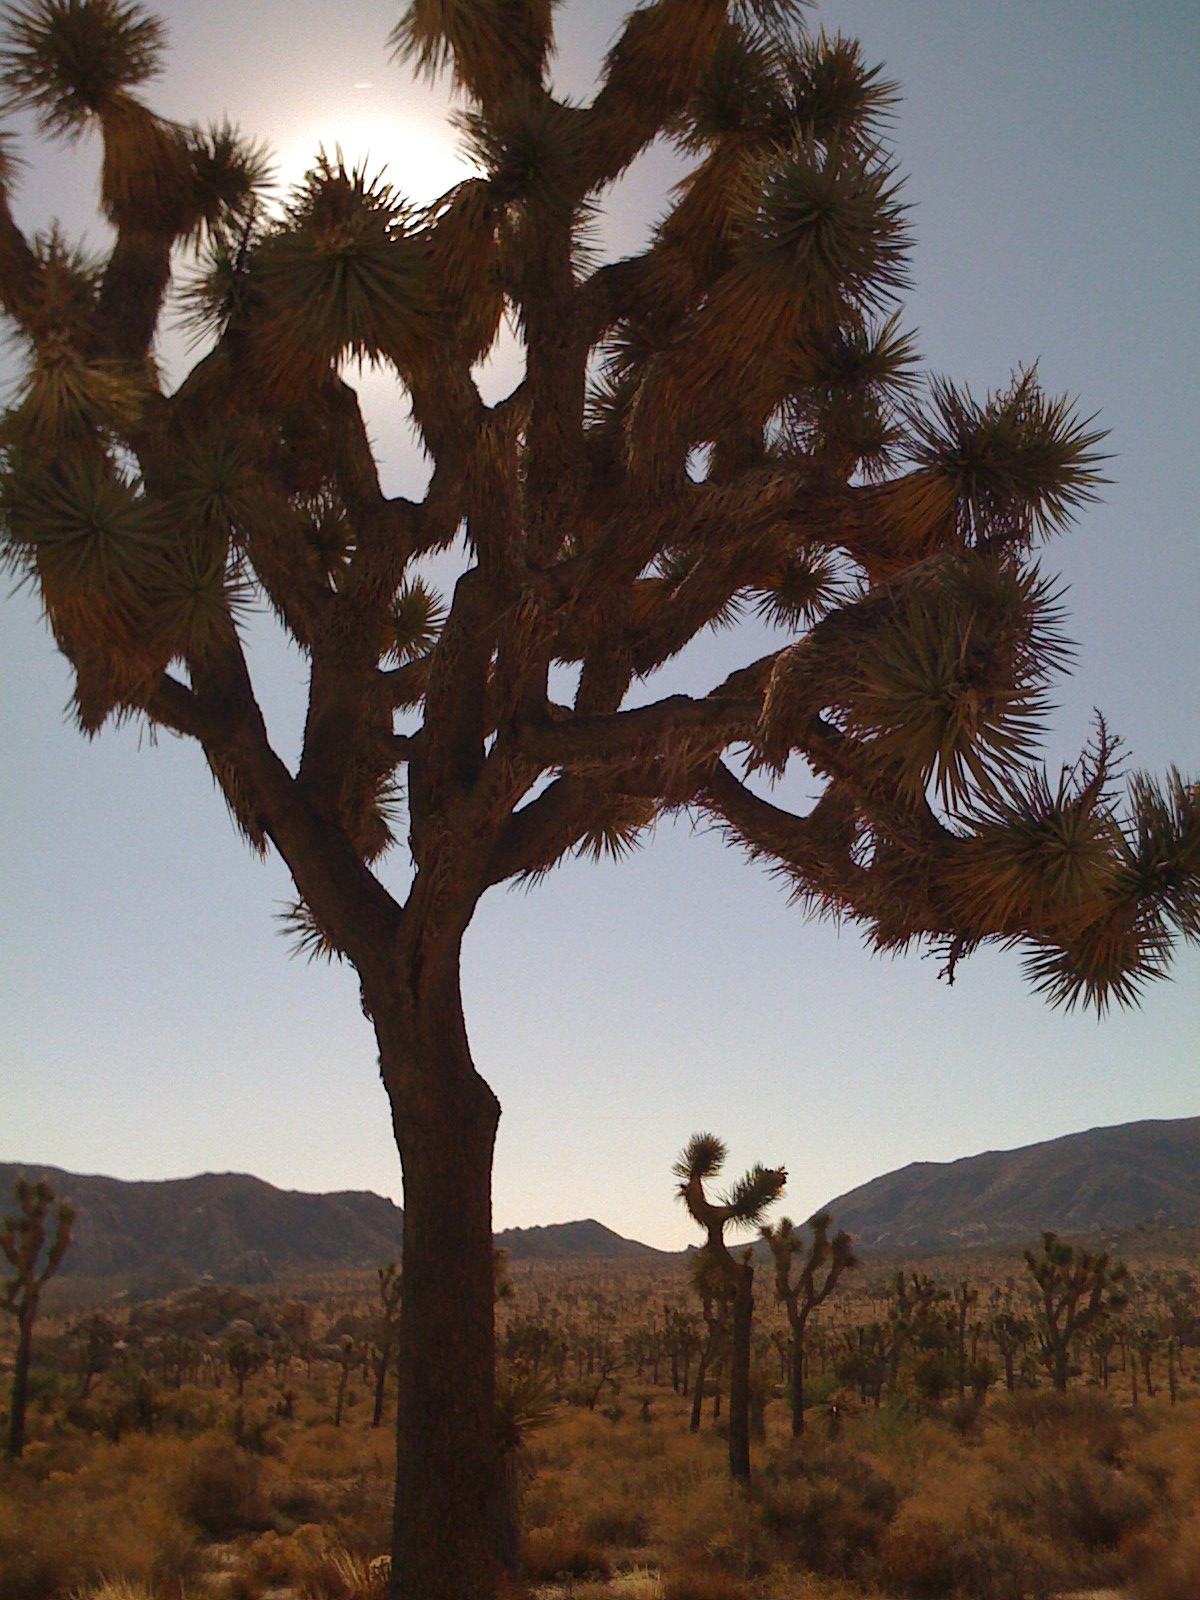
\includegraphics[width=.5\linewidth]{gfx/sagmeisterJoshuaTrees}}
	\end{center}
		\caption[Joshua Trees \newline \citep{Sagmeister:2008}]{Joshua Trees, die einzigen Schattenspender in der Mojave Wüste, gelten als Leitbilder für das Joshua Tree Principle, welches die Wirkungsweise von Guiding Principles beschreibt.}\label{fig:sagmeisterJoshuaTrees}
\end{figure}

Um die Wirkungsweise von Guiding Principles (im Sinne von Memen) zu veranschaulichen, soll eine kurze Geschichte helfen. 

\begin{quote}
	\textsl{>>Vor nicht all zu langer Zeit reiste ich durch die Wüstenlandschaften von Kalifornien, Arizona, Nevada und Utah. Dabei passierte ich einen Teil der Mojave Wüste, welche die 4 Bundesstaaten verbindet. Die Besonderheit dieser Wüstenlandschaft sind die dort wachsenden Joshua Trees\index{Joshua Trees} [vgl. \autoref{fig:sagmeisterJoshuaTrees}]. Sie waren seit jeher für die Einheimischen sehr wertvoll, da sie in der endlos scheinenden Wüstenlandschaft Schatten spendeten, wie mir der Tourguide erklärte. Bevor jedoch die Reiseleitung überhaupt begonnen hatte über die Joshua Trees zu sprechen, wusste ich bereits über sie Bescheid und erkannte sie. Nicht weil ich in meiner Freizeit Naturbücher auswendig lerne, sondern weil ich ironischer weise kurz vor meinem Reiseantritt ein Buch über Design von der Autorin Robin Williams gelesen habe. Sie beschreibt in ihrem Buch ein Prinzip auf welches ich mit meiner Geschichte ebenfalls hinzielen möchte: The Joshua Tree Principle. Wäre ich vor meiner Reise bereits in dieser Region unterwegs gewesen, wären mir die Bäume mit großer Sicherheit nie aufgefallen. Doch kaum wusste ich den Namen, wurde mir der Baum bewusst.<<}
\begin{flushright}\citep{Sagmeister:2008}\end{flushright}
\end{quote}

Genau das ist auch der Punkt:

\begin{quote}
	\textsl{>>Once you can name something, you’re conscious of it. You have power over it. You own it. You’re in control.<<}
\begin{flushright}\citep{Williams:1994}\end{flushright}
\end{quote}

Dawkin möchte ebenfalls mit dem Begriff Memen auf dieses Phänomen hinzielen: 

\begin{quote}
	\textsl{>>A meme should be regarded as a unit of information residing in a brain.<<}
	\begin{flushright}\citep{Dawkins:1982}\end{flushright}
	\smallskip
	\textsl{>>Meme can propagate themselves from brain to brain, from brain to book, from book to brain, from brain to computer, from computer to computer.<<}
	\begin{flushright}\citep{Dawkins:1986}\end{flushright}
\end{quote}

Durch das Wissen um Guiding Principles und die Fähigkeit sie benennen zu können, sollte es uns also möglich sein, sie kontrolliert einzusetzen, um das richtige Design zu kreieren. Wie kommt es dann aber, dass schlechtes Design keine Seltenheit ist? Guiding Principles sind Meme, die Designer in ihr Konsortium, welches aus vielen Memen besteht, aufnehmen. Abgesehen davon, dass Guiding Principles nur in bestimmten Kontexten wirken, können Entwickler Meme besitzen, die sie daran hindern ein gutes Design zu erstellen. Das können z.B. Meme über die Unternehmensorganisation, die Arbeit an sich oder das Umfeld sein. Das >>Sammeln<< von Memen, die zu einem guten Design führen, ist ein Lernprozess und unterscheidet somit ausgebildete Designer von Nicht- Designern. \\
Da nun klar ist, was Guiding Principles sind und wie sie wirken, wird in weiterer Folge auf einige Prinzipien des Interface Designs eingegangen. Über die Jahre wurden viele Design Prinzipien oder auch sog. Goldene Regeln des Designs entwickelt. Ihr Ursprung liegt dabei in der Psychologie und im Sammeln praktischer Erfahrungen. Ein Vorreiter auf diesem Gebiet war der Kognitionswissenschafter und Informatikprofessor Don Norman, der bereits 1988 mit seinem Bestseller The Design of Everyday Things \citep{Norman:1988} auf die Schwächen und Stärken von Designs hindeutete. Viele Designer und Autoren wie Williams, Shneiderman, oder Benyon bauten auf diese auf und erstellten darauf hin ihre eigenen aus Erfahrungen zusammengetragenen Prinzipien - einige vage, einige detaillierter formuliert. Angewendet, sollen sie im Allgemeinen helfen ein System zu lernen, das Gefühl geben stets die Kontrolle zu haben und vor Unsicherheit vorbeugen.

\begin{small}
\begin{enumerate}
	\item \emph{Bewahre die Konsistenz}\index{Guiding Principles!Konsistenz} - Diese Regel ist die meist missachtete. Unter anderem vielleicht weil es viele verschiedene Formen der Konsistenz gibt. Konsistenz sollte bei Standardoperationen und Repräsentationen, sowie bei der Benützung von Metaphern eingesetzt werden – innerhalb Applikationen und zwischen Applikationen. Sie hilft den	Benutzer ein mentales Modell eines Systems zu erstellen und es zu erhalten.\\
Ähnliche Situationen erfordern konsistente Aktionsabläufe; Bezeichnungen sollten in	Eingabeaufforderungen, Menüs und in der Hilfefunktion ident sein; Auf gleiche Farben, Layouts, Großschreibungen, Schriftarten usw. sollte durchgehend geachtet werden. Ausnahmen, wie das >>Nichtzeigen<< von Passwörtern oder das Bestätigen von Löschaktionen, sollten in ihrer Anzahl minimal gehalten werden.
	\item \emph{Gib Feedback}\index{Guiding Principles!Feedback} - Biete dem Benutzer für jede Aktion (so schnell wie möglich) genügend informatives Feedback, um ihm zu zeigen welchen Effekt seine Aktion hat. Für kleine, häufige Aktionen kann die Rückmeldung bescheiden ausfallen, wobei bei seltenen Haupttätigkeiten ein umfangreicheres Feedback gegeben werden sollte.
	\item \emph{Entwickle für Fehlverhalten}\index{Guiding Principles!Fehlverhalten} - Eine übliche Ausrede für auftretende Systemprobleme, ist das menschliche Fehlverhalten. Da irren jedoch menschlich ist, und Menschen Fehler machen müssen um zu lernen, sollte ein System so gut wie möglich designed werden, um	ernste Fehler zu vermeiden bzw. das Auftreten von Fehler so gering wie möglich zu halten. Beispiele wären Auswahlmenüs um Formulare auszufüllen oder das Ignorieren von	Buchstaben in numerischen Eingabefeldern. Falls Fehler trotzdem gemacht werden,	sollten simple, konstruktive Anweisungen geboten werden um das Problem zu lösen. Man	spricht hierbei auch von >>guten Fehlermeldungen<<.
	\item \emph{Zeig Toleranz}\index{Guiding Principles!Toleranz} - Gestatte Benutzern ihre Aktionen, insbesondere Fehler rückgängig zu machen. Diese Funktion nimmt die Angst von den Usern und ermutigt sie zur Erforschung von neuen Optionen.
	\item \emph{Übergib die Kontrolle}\index{Guiding Principles!Kontrolle} - Benutzer haben das Verlangen stets die Kontrolle über das	System zu haben. Unerwartete Systemaktionen führen zu Angst und Unbehagen. Deswegen sollte immer klar gemacht werden wer oder was gerade die Kontrolle besitzt,	um an das Vertrauen des Benutzers zu gelangen.
	\item \emph{Vereinfache die Programmstruktur}\index{Guiding Principles!Programmstruktur} - Laut dem Psychologen George Miller können sich	Menschen maximal 7±2 verschiedene Informationen merken (laut mancher Literatur sogar weniger). Er spricht dabei auch von der magischen Zahl 7\index{Die magische Zahl 7}. Aus diesem Grund sollte die Beanspruchung des Kurzzeitgedächtnisses minimal gehalten werden. Viele Entwickler halten sich strikt an diese Zahl z.B. beim Anzeigen von Items, vergessen jedoch, dass die Information meistens sowieso am Bildschirm zu sehen ist. Auf die Informationen kann also stets zurückgegriffen werden, ohne sie sich merken zu müssen. Es ist also nicht nötig Millers Theorie wörtlich im Design zu übernehmen, jedoch sollte eine Anwendung immer nur so komplex wie nötig und nicht wie möglich sein. Ein Beispiel wäre das Versenden einer Email. Die benötigte Information hierbei ist die Absender- und Empfängeradresse. Es wäre jedoch unnötig die Absenderadresse jedes Mal erneut einzugeben - Der Email-Client kümmert sich darum. Die Komplexität wurde somit aus der Sicht des Benutzers verringert.
	\item \emph{Vermittle Vertrautheit}\index{Guiding Principles!Vertrautheit} - Sprache und Symbole sollten immer so gewählt werden, damit sie für den Benutzer vertraut wirken. An Stellen wo dies nicht möglich ist, weil die	Konzepte so sehr von dem abweichen was die Benutzer kennen, sollten Metaphern verwendet werden (Beispiel: Papierkorb am Desktop). Sie stellen eine Verbindung zu bestehenden Wissen, einer vertrauten Quelle her. Im Allgemeinen sollten Elemente so	designed werden, dass immer Klarheit herrscht wofür sie stehen. Buttons müssen z.B.	aussehen wie Buttons, damit Benutzer wissen, dass man sie drücken muss.
	\item \emph{Achte auf Sichtbarkeit}\index{Guiding Principles!Sichtbarkeit} – Es sollte stets sichergestellt werden, dass Elemente sichtbar sind, damit der Benutzer sehen kann welche Funktionen verfügbar sind und mit welcher Aufgabe das System gerade beschäftigt ist. Dies basiert auf der psychologischen Grundregel, dass es einfacher ist etwas zu erkennen als sich daran erinnern zu müssen.
	\item \emph{Erstelle Grenzen}\index{Guiding Principles!Grenzen} - Grenzen sollen Benutzern das Gefühl geben, dass es nur einen möglichen Weg gibt - den richtigen natürlich. Sie bewahren User davor, unangebracht zu handeln indem sie ernste Fehler durch >>normale<< Tätigkeiten hervorrufen.\\
	Und schlussendlich..
	\item \emph{Sei freundlich}\index{Guiding Principles!Freundlichkeit} – Interaktive Systeme sollten höflich, freundlich, und angenehm gestaltet sein. Nichts ruiniert die Erfahrung mit einer Anwendung mehr als eine aggressive Mitteilung oder abrupte Unterbrechungen.
\end{enumerate}
\end{small}
\citep{Benyon:2005, Preece:1994, Saffer:2007, Shneiderman:1998}

\section*{Zusammenfassung}
Design ist ein alltäglicher und weitgehender Begriff, der sowohl Bedeutung als Tätigkeit und als Repräsentation in sich trägt. Es gibt viele verschiedene Designdisziplinen welche zur Unterscheidung von Kompetenzen professioneller Designer dienen. Ein wichtiger Bereich für Softwaredesign ist (User) Interface Design bzw. Interaction Design, welche sich besonders mit den subjektiven und qualitativen Aspekten, bei der Interaktion von Menschen und Computer, beschäftigen. Es gibt verschiedenste Methoden, die benutzt werden können um Designprobleme zu verstehen und um nötige Lösungsstrategien zu entwickeln. Skizzen bieten durch ihre minimale Detailstufe und der kurzen Herstellungszeit Mehrdeutigkeiten, die zum Weiterforschen und Kommentieren anregen. Dieser soziale Prozess ist wichtig in der Ideenfindung am Anfang einer Designphase. Prototypen verbinden alle Teile eines Designs, zu einer Einheit und verschaffen im (User) Testing neue Einblicke. Beobachtungen von Verhaltensmustern innerhalb der Testings bewegen schlussendlich dazu das Design iterativ zu überarbeiten. Es kann zusätzlich auch nützlich sein, sich durch Personas und Szenarien eine Art Leitfaden zusammen zu stellen, der durch das Beleuchten von Tätigkeiten potentieller Benutzer zustande kommt. Dieser sollte aber ständig vervollständigt werden, da er meist Lücken aufweist. Es gibt kein Rezept für das \emph{richtige} Design, jedoch entstanden über die Jahre sog. Guiding Prinicples oder Leitfäden, die Designern helfen sollen bessere Systeme zu entwickeln. \\
Design hängt immer mit der Kommunikation und Interaktion von Personen zusammen und ist somit eine >>soziale Konstruktion einer technischen Realität<<. Das folgende Kapitel soll nun näher auf den kollaborativen Charakter eingehen.


%*************************************************************
\chapter{Kollaboratives Design}\label{ch:kollaborativesDesign}
%*************************************************************

lorem ipsum

\section*{Zusammenfassung}
lorem ipsu
%*************************************************************
\chapter{Design VS Computer}\label{ch:DesignVSComputer}
%*************************************************************

Menschen arbeiten mit Dokumenten in zwei verschiedenen Welten: der elektronischen Welt des Computers und der physikalischen Welt am Schreibtisch. Jede Welt hat ihre Vor- und Nachteile (siehe \autoref{tab:wellnerDokumente}), welche uns dazu bewegen die >>richtige<< für bestimmte Aufgaben zu wählen \citep{Wellner:1993}.

\begin{table}
    \myfloatalign
\begin{tabularx}{\textwidth}{p{5cm}X}
    \toprule
	    \tableheadline{Elektronische Dokumente} & \tableheadline{Papierdokumente}
	     \\ \midrule
		\begin{itemize} 
			\item{schnelles Editieren}
			\item{schnelles Kopieren}
			\item{schnelles Senden}
			\item{schnelles Freigeben}
			\item{schnelles Ablegen}
			\item{schnelles Abrufen}
			\item{erlaubt Stichwortsuche}
			\item{erlaubt \newline Rechtschreibprüfung}
			\item{erlaubt sofortige \newline Berechnungen}
		\end{itemize} &
		\begin{itemize} 
			\item{3-dimensional}
			\item{überall akzeptiert}
			\item{billig}
			\item{portabel}
			\item{geläufig}
			\item{hochauflösend}
			\item{einfach zu lesen}
			\item{fühlbar}
			\item{man kann beide \newline Hände \& Finger \newline zum bearbeiten \newline verwenden}
			\item{man kann mit einem Stift darauf kritzeln}	
		\end{itemize}
	\\  \bottomrule
\end{tabularx}
  \caption[Elektronische Dokumente und Papierdokumente \newline \citep{Wellner:1993}]{Gegenüberstellung der Eigenschaften von elektronischen Dokumenten und Papierdokumenten.}
  \label{tab:wellnerDokumente}
\end{table}

\begin{figure}
        \myfloatalign
        \subfloat[Geschriebene Darstellung (in der Wortebene).]
        {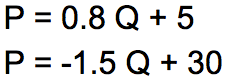
\includegraphics[width=.48\linewidth]{gfx/johnsonDarstellungsformenB}} \quad
        \subfloat[Graphische (schematische) Darstellung.]
        {\label{fig:johnsonDarstellungsformenB}%
         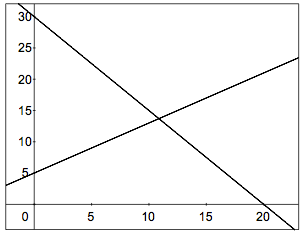
\includegraphics[width=.48\linewidth]{gfx/johnsonDarstellungsformen}} \\
        \caption[Darstellungsformen \newline \citep{Johnson:2009}]{Die schematische Darstellung (a) und die Darstellung in der Wortebene (b) eines mathematischen Verhältnisses. Beide Darstellungsformen zeigen die gleiche Information. }\label{fig:johnsonDarstellungsformen}
\end{figure}

\medskip In mancher Hinsicht scheint es aber, als wäre Papier bald obsolet. Manche prophezeien das papierlose Büro schon in wenigen Jahren. Das Eigenartige dabei ist nur, dass sich die Leute ungern von Papier trennen. Studien belegen, dass der Papierkonsum in Büros seit 1970 um das 6-fache anstieg und derzeit jährlich um 20\% steigt \citep{seybold:1992}. Papier hat ebenso wie elektronische Dokumente Eigenschaften, die Menschen nicht aufgeben wollen. Das macht sie in Hinsicht auf computerbasierende Alternativen >>unverwüstlich<<. \citep{Luff:1992} 

\medskip Wie wichtig Papier (im Zusammenhang mit Skizzen) für Designer ist, wurde auch im Kapitel \nameref{ch:designTheorie} beschrieben. Welchem Umstand dies das alte Medium zu verdanken hat, lässt sich laut Sellen und Harpers Arbeit \emph{The Myth of the Paperless Office} \citep{Sellen:2003} nicht durch einfache Merkmalgegenüberstellungen herausfinden. Nur Studien und Observationen können das kognitive Verhalten bei der Benutzung von Papier und digitalen Artefakten beschreiben. 

\medskip Das nun folgende Kapitel soll die Stärken und Schwächen traditioneller und digitaler Arbeitsweisen gegenüberstellen und mittels verschiedenster Studien eine Erklärung zum oben genannten Phänomen finden. %-- Können die beiden Welten von einander lernen?
%Deswegen initierten Terrenghi et al. eine Designstudie, die dabei helfen sollte, das kognitive Verhalten bei der Benutzung von Papier und digitalen Artefakten zu beschreiben. \citep(Terrenghi:2007) Ihre Ergebnisse sollen in den nächsten beiden Abschnitten erläutert werden.

\section{Skizzieren auf Papier} \index{Skizzen!auf Papier}
%Skizzieren erlaubt Personen mit abstrakten und ungenauen Elementen zu arbeiten, diese daraus resultierenden oft mehrdeutigen Kritzeleien wiederholt zu interpretieren und alternative Bedeutungen zu erlangen. Skizzierte Abbildungen, Bilder und Karten helfen Personen ihre Gedanken zu manifestieren oder Ideen anderen zu erklären. \citep{YiLuenDo:2005}
Skizzieren fördert eine schnelle und formlose Informationsverarbeitung. Eine Telefonnummer würde man beispielsweise eher auf ein Whiteboard in der Nähe des Schreibtischs schreiben, als sie in den Computer einzugeben, schnelle Berechnungen oder \emph{To-Do-Lists} auf einem Blatt Papier, da sie leicht zu erstellen sind und das Ergebnis portabel ist.
Larkin und Simon verglichen \emph{schematische} Darstellungen mit \emph{Darstellungen in der Wortebene} (geschrieben oder gesprochen) und zeigen damit dass räumliche Darstellungen oft mehr aussagen, als die gleiche Information in einem ausführlich geschriebenen Statement \citep{Larkin:1987}. Wie effizient Information verarbeitet werden kann, hängt technisch betrachtet davon ab, wieviel >>Rechenaufwand<< von Nöten ist, um Vorgaben so zu übersetzen, damit Verständnis entsteht. Um beispielsweise einen mathematischen Ausdruck eines Verhältnisses zu beschreiben, würde sich eine schematische Darstellung besser eignen. Der gleiche Ausdruck als Darstellung in der Wortebene würde eine längere Berechnungszeit benötigen (siehe \autoref{fig:johnsonDarstellungsformen}).

\medskip Wenn Personen skizzieren, fassen sie relevante Informationen zusammen und lassen die irrelevanten aus \citep{Tversky:2002}. Zeichnen erlaubt Personen Papier als externen Speicher zu verwenden, um ihre kognitive Belastung zu verringern. Schematische Darstellungen stellen ein vereinfachtes Abbild von Informationsbereichen dar \citep{Tversky:2000}. Per Hand gezeichnete Landkarten bzw. Wegbeschreibungen, werden z.B. mit simplen Formen wie Rechtecke oder Kreise für Gebäude, Linien oder Pfeile für Wege und sich überschneidende Linien für Kreuzungen gezeichnet \citep{Tversky:1999}. Die Form und Krümmung von Gebäuden und Linien werden lediglich geschätzt, da Menschen bei genau gezeichneten Karten Schwierigkeiten haben, die kleinen Unterschiede zwischen der Karte und der echten Welt abzugleichen. Räumliche Darstellungen sind ein beeindruckendes Hilfsmittel beim Lernen. Skizzieren erlaubt Lernenden Konzepte, so wie sie verstanden wurden, aufzuzeichnen und diese von erfahrenen Personen auf Inkonsistenzen und Fehlern überprüfen zu lassen \citep{Forbus:2008}.
%Van Sommers studierte ausgiebig das Zeicheinverhalten von Personen \citep{VanSommers:1984}. 

\medskip Goel führte in \citep{Goel:1995} eine Reihe an Experimenten durch, um die kognitiven, handlungsauffordernden Merkmale von Skizzen zu erforschen. In seinen Studien verglich er traditionelle Papier-und-Stift Skizzen mit Skizzen, die mit Hilfe von computerbasierten Zeichenprogrammen erstellt wurden. Die teilnehmenden Designer bekamen Anweisungen, ein Artefakt auf beide Arten zu designen. Dabei kam ein modifiziertes Softwaretool zum Einsatz, das lediglich strukturierte Eingaben, wie gerade Linien, Rechtecke und Ellipsen unterstützte. \graffito{Skizzieren mit einem strukturierten Softwaretool kommt nicht an die Schnelligkeit von unstrukturierten Papier-und-Stift Skizzen heran.} Die Ergebnisse zeigten, dass das strukturierte Computerprogramm bezüglich der Ideenfindung nicht an die Schnelligkeit vom unstrukturierten Papier-und-Stift System herankam. Skizzieren unterstützt Designer bei der schnellen Entwicklung vieler unterschiedlicher Ideen. Diesen explorativen Charakter von Skizzen beschrieb Goel als \emph{Quertransformationen}, die sich im Gegensatz zu den \emph{vertikalen Transformationen}, welche sich durch Verfeinern von Ideen auszeichnen, deutlich abgrenzen. Bei den beiden Transformationstypen stützt sich Goel auf die von Newman und Landay in \citep{Newman:2000} beschriebenen Aktivitäten verschiedener Designstufen. Am Anfang des Designprozesses sind Designer mit der Ideengenerierung und -findung beschäftigt (Quertransformationen). Später konzentrieren sich Designer schrittweise Überarbeitungen und Änderungen (vertikale Transformationen).

\medskip 

\section{Skizzieren am Computer} \index{Skizzen!am Computer}

Heutige stiftbasierte Hardware orientiert sich vorwiegend am Schreiben und Lesen von Text. Wenn man erwägt, diese auch für Designaktivitäten einzusetzen, sollte man sie mit den Werkzeugen, die Designer in der Praxis benutzen, vergleichen. 

Designer können schnell Zeichnungen auf Papier anfertigen und zwischen den einzelnen Seiten blättern. Sie können ebenfalls die Zeichnungen nebeneinander an die Wand heften, um sie zu vergleichen. Die Stiftspitze zeichnet dabei sofort bei Berührung auf dem Papier und es können zwei Hände benutzt werden um das Blatt Papier nach Belieben zu drehen bzw. um Hilfsmittel wie ein Lineal zu halten.

\medskip Am einfachsten wäre es, wenn computerunterstützes Skizzieren genau die selben Eigenschaften aufweisen würde. Jedoch mangelt es der derzeitigen Hardware an Portabilität, schnellem Reaktionsvermögen und dem vertrauten Gefühl traditioneller Designpraktiken. Die kommerzielle Entwicklung und Forschung verbessert kontinuierlich Hardware auf diesem Sektor, so unterstützen viele Geräte wie z.B. PDAs, Tablet PCs oder interaktive Wandinstallationen bereits eine Art von Stift- oder Touchinput. Während stiftbasierte Systeme seit Jahrzehnten bei Forscher im Einsatz sind, verbreiten sie sich erst seit Mitte der 90er Jahre und werden stetig billiger.

\medskip >>Skizzierhardware<<\index{Skizzierhardware} kann in zwei Gruppen unterteilt werden: 
\begin{itemize}
	\item{Hardware, die nur Eingaben unterstützt und}
	\item{Hardware, die Eingaben und Ausgaben unterstützt.}
\end{itemize}

Tablets\index{Tablets} geben den Benutzern die Möglichkeit, mit Hilfe eines Eingabestifts zu schreiben bzw. zu zeichnen. Manche beschränken sich dabei aber lediglich auf die Eingabe und zeigen nicht gleichzeitig das Gezeichnete. Geräte, die Ein- und Ausgaben unterstützen, haben sich besonders bei den Tablet PCs durchgesetzt. Zusätzlich gibt es auch Systeme, die das gezeichnete indirekt >>scannen<<. Z.B. entwickelte PARC das ScanScribe System, welches Zeichnungen analysiert, die mit herkömmlichen Stift und Papier erzeugt wurden und erstellt daraus eine mit dem Computer aufgebesserte Version. \citep{Johnson:2009}

\subsection{Electronic Ink} \index{Electronic Ink|textbf}
Wenn man eine Zeichnung mit künstlerischem Ausdruck zu Papier bringt, gibt es viele Faktoren die das Endergebnis beeinflussen. So z.B. die Stärke des Schreib- bzw. Zeichengeräts, sowie die Materialeigenschaften des Papiers. In vielen Branchen, wie beispielsweise in der Computeranimation, ist es noch immer üblich, Illustrationen zuerst auf Papier zu zeichnen und danach schrittweise zu digitalisieren. Es wurden zwar einige Versuche gestartet, direkt auf digitaler Ebene zu zeichnen, jedoch wird dies nach wie vor hauptsächlich nur dort verwendet, wo der Computer nicht nur optional benutzt wird. \citep{Henzen:2005}

Viele Tablets sind druckempfindlich. Designer benutzen oft stärkere Linien, um Objektgrenzen hervorzuheben und dünne Linien um dezente Texturen, Schatten oder Rundungen anzudeuten. Geräte, die Druck messen können, erlauben Designer dickere oder dunklere Striche zu zeichnen, ohne vorher in einen anderen Zeichenmodus wechseln zu müssen.

Die Druckmessung\index{Electronic Ink!Druckmessung} wurde auf verschiedene Weisen umgesetzt. Z.B. durch zwei übereinander liegenden leitfähigen Schichten mit entgegengesetzten Stromrichtungen. Die Schichten berühren sich nicht und sind oft durch eine nicht leitende Flüssigkeit abgeschirmt. Wenn etwas (ein Stift oder Finger) die obere Schicht berührt, verändert sich die Spannung und die Position kann mittels Interpolation an den Kanten errechnet werden. Andere berührungsempfindliche Oberflächen messen die elektrischen Eigenschaften der Dinge, die sie berühren. Darum funktionieren auch Handschuhe auf manchen Laptop Trackpads nicht. Wacom\texttrademark{} Tablets und gleichartige induktive Geräte, benötigen spezielle Stifte, die in einem vom Tablet generierten elektromagnetischen Feld mitschwingen. Wieder andere Tablets erkennen akkustische oder optische Störungen zur Positionsberechnung.

Es gibt Oberflächen, die lediglich die Koordinaten eines einzigen Berührungsortes liefern können und Oberflächen, die mehrere erkennen. Diese werden auch Multitouchoberflächen genannt. Multitouchsysteme, wie z.B. \emph{Hans's Frustrated Total Internal Reflection technique} \citep{Han:2005} und \emph{Microsoft's Surface System} \citep{Surface:2010} befinden sich derzeit im Aufschwung, werden aber mit den Fingern order Händen benutzt und bieten deswegen völlig andere Anwendungserlebnisse als Stiftbasierte Oberflächen.

\subsection{Der Unterschied zwischen Eingabestift und Maus} \index{Eingabestifte} \index{Mäuse}

Egal welche Abtasttechnologie man wählt, alle oben genannten Geräte erlauben Benutzern eine Eingabevariante, die näher an das traditionelle Schreiben herankommt, als die Maus jemals könnte. Obwohl Stift- und Mauseingaben viele Eigenschaften teilen (beide erlauben Benutzer im 2D Raum zu interagieren), haben sie einige grundlegende Unterschiede.

\medskip Mauseingaben liefern Daten über die \emph{Bewegung}, Stifteingaben liefern Daten über die \emph{Position} \citep{Hinckley:2002}. Mit anderen Worten produzieren Mäuse relative \emph{Änderungen} in der (x,y) Position und Stifte direkte, absolute (x,y) Positionen. Benutzer können Tablets aber auch so konfigurieren, damit sie sich wie Mäuse verhalten und relative Positionen erzeugen.

\medskip Die Form der Geräte ist ebenfalls extrem wichtig. Ein Stift zwingt die Benutzer die Feinmotorik ihrer Finger einzusetzen um die Stiftspitze zu steuern, wohingegen die Hand- und Unterarmmuskeln die Maus steuern. Finger können zwar auch zur Maussteuerung benutzt werden, aber nicht mit der gleichen Fertigkeit. Je nach Art der Arbeit ist ein Stift ergonomisch besser als eine Maus oder umgekehrt.

Tablets können aber mehr als nur die Stiftposition erkennen. Manche Geräte können auch den Aufpressdruck, den Winkel oder die Rotation des Stifts messen. Das andere Ende des Stifts wird auch oft als alternativer Modus (z.B. als ein Radierer) benutzt. 

Einige Stifte haben noch zusätzliche Buttons. Während Buttons unentbehrliche Bestandteile von Mäusen sind, können sie entlang des Stiftgehäuses schwer benutzbar sein \citep{Plimmer:2008}. Die Kraft, die bei einem Buttonklick an der \emph{Maus} entsteht, ist orthogonal zu der Oberfläche, auf der die Maus benutzt wird und beeinflusst die Zielgenauigkeit nur unwesentlich. Ein Knopfdruck am \emph{Stift} hingegen kann die Stiftspitze ungewollt bewegen, was das Zeigen auf ein \graffito{Buttons an Tabletstiften können schwer benutzbar sein und sich auf längere Zeit unangenehm auswirken.}bestimmtes Objekt und das gleichzeitige Drücken einer Taste erschwert (siehe \autoref{fig:johnsonButtonPress}). Zudem muss der Benutzer beim Drücken einer Taste üblicherweise den Stift erst so drehen, damit sich sein Finger wieder über der Taste befindet (was durchaus öfter vorkommt). Diese Aktion lenkt ab und ist auf längere Zeit gesehen unbequem. \citep{Johnson:2009}

\begin{figure}
        \myfloatalign
        \subfloat[Drücken einer Maustaste erzeugt eine Kraft, die orthogonal auf die darunterliegende Oberfläche wirkt.]
        {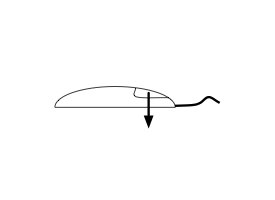
\includegraphics[width=.48\linewidth]{gfx/johnsonMousePress}} \quad
        \subfloat[Drücken einer Stifttaste erzeugt eine ungewollte Stiftspitzenbewegung.]
        {\label{fig:johnsonButtonPressB}%
         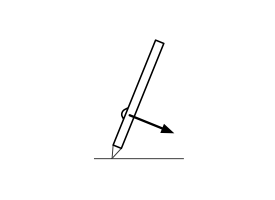
\includegraphics[width=.48\linewidth]{gfx/johnsonStylusPress}} \\
        \caption[Kräfte bei Buttonklicks. \newline \citep{Johnson:2009}]{Entstehende Kräfte beim Drücken einer Maustaste (a) und einer Stifttaste (b) eines Tablets.}\label{fig:johnsonButtonPress}
\end{figure}
\clearpage

\subsection{Interaktionstechniken für stiftbasierte Skizziersysteme} \index{Skizziersysteme!Interaktionstechniken}
Bei der Entwicklung neuer Technologien ist es wichtig das Ausmaß der kognitiven Belastung des Tools zu berücksichtigen. Aus Oviatt's Studie \citep{Oviatt:2006} über Mathematikstudenten geht hervor, dass das Arbeiten mit stiftbasierte Applikationen auf Tablet PCs erheblich schlechter funktioniert als mit herkömmlichen Stift und Papier. Durch die Benutzung der Tablets benötigten die Studenten mehr Zeit bei der Lösung von Mathematikaufgaben, was dazu führte dass sie sich mit der Technologie nicht anfreunden konnten. Anthony et al. führten eine ähnliche Studie durch, in der sie Eingaben von Studenten verglichen, die Gleichungen beinhalteten. Zur Eingabe dienten ein \emph{Standard \acs{WIMP}\index{WIMP}\footnote{Die Abkürzung WIMP wurde 1980 von Merzouga Wilberts ins Leben gerufen und steht für Window, Icon, Menu, Pointing Device. Es bezeichnet das Grundkonzept moderner grafischen Benutzerschnittstellen (\acp{GUI}).} Interface} und ein Eingabetablet \citep{Anthony:2005}. 

Sie kamen zur Erkenntnis, dass die Studenten Stifteingaben bevorzugten und \graffito{Umso mehr Aufmerksamkeit man (Software-)Tools schenken muss, desto weniger Aufmerksamkeit bekommt das eigentliche Problem.}handgeschriebene Gleichungen schneller und genauer niederschreiben konnten, als mit Keyboard und Maus. Papier und Stift wurden dem elektronischen Schreiben zwar vorgezogen, jedoch waren ihnen Stifte im Allgemeinen lieber als Tastatur- und Mauseingaben. Beide Studien kamen zum selben Schluss: Je mehr Aufmerksamkeit Benutzer aufbringen müssen um das Tool zu verwenden, desto weniger Aufmerksamkeit schenken sie dem eigentlichen Problem.

\medskip Zur Redzuierung der kognitiven Belastung\index{Skizziersysteme!Kognitive Belastung} müssen demnach natürlichere Interaktionstechniken entwickelt werden. Verschiedenste Methoden erwiesen sich bis dato durchaus brauchbar zum effizienten Arbeiten mit Stiftapplikationen. Kontextmenüs sind ein gutes Beispiel dafür \citep{Kurtenbach:1991}. Traditionelle Menüs zeigen eine Liste an Optionen, welche das Menü nach unten und rechts wachsen lassen. Bei Tablets, die Eingaben und Ausgaben unterstützen (z.B. Tablet PCs) kann dies dazu führen, dass Benutzer das Menü mit der Hand verdecken. >>Torten<<-Menüs (eine Art Kontextmenü) erscheinen zentriert um die Stiftposition und zeigen die Optionen kreisförmig (siehe \autoref{fig:johnsonPieMenu}). Die Hand ist zwar bei dieser Art von Menüs noch immer teilweise im Weg, aber zumindest ist ein Teil des Menüs dadurch sichtbar. Der Vorteil dieser Methode ist, dass sich Personen Gesten anlernen können, ohne die Menüeinträge jedesmal erneut lesen zu müssen. Voraussetzung dafür ist jedoch, dass sich die Menüeinträge niemals ändern. Eventuell schwindet auch der Bedarf eines visuellen Menüs durch die Gesten. Tortenmenüs werden in Applikationen wie Maya \citep{Maya:2010}, Spielen wie The Sims \citep{EA:2010} oder als Erweiterungen in Webbrowser verwendet. Der Ansatz funktioniert zwar gut, bringt aber auch zwei Nachteile mit sich. Zum einen ist es nicht klar wie man das Menü aufrufen kann und zum anderen müssen Gesten erst entdeckt, erlernt und ins Gedächtnis gerufen werden.

\begin{figure}
        \myfloatalign
        \subfloat[Tortenmenüerweiterung für den Firefox Webbrowser.]
        {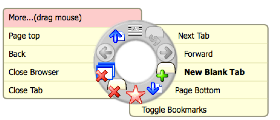
\includegraphics[width=.48\linewidth]{gfx/johnsonPieMenuFF}} \quad
        \subfloat[Autodesk Maya Tortenmenü.]
        {\label{fig:johnsonPieMenuB}%
         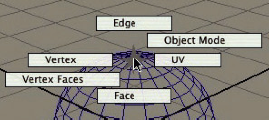
\includegraphics[width=.48\linewidth]{gfx/johnsonPieMenuMaya}} \\
        \caption[Tortenmenüs \newline \citep{Johnson:2009}]{Tortenmenüs in Firefox (a) und Maya (b).}\label{fig:johnsonPieMenu}
\end{figure}

\medskip Ramos et al. \citep{Ramos:2004} erforschte weiters die Benutzung von Aufpressdruckdaten bei stiftbasierenden Interaktionen. Zu der zweidimensionalen (x,y) Stiftposition kommt die Druckstärke des Stiftes als dritte Dimension hinzu, die der Benutzer frei verändern kann. Zum Beispiel kann ein leichter Druck ein Menü zeigen und ein harter Druck ein anderes Menü. Druck kann eine effektive Eingabeart sein, wenn sie richtig (mit haptischen und visuellen Feedback) eingesetzt wird.

\medskip Hinckley et al. \citep{Hinckley:2005} empfiehlt die Benutzung von \emph{Begrenzer} um Kontextmenüs aufzurufen. \emph{Begrenzer} sind Eingaben, die Benutzer normalerweise nicht zeichnen würden aber dennoch leicht zu merken sind. Ein Beispiel zeigt ihr System Scriboli, in dem ein >>Rattenschwanz<< (eine Schleife am Ende einer Selektionsgeste) als Begrenzer benutzt wird. Diese flüssige Bewegung lässt den Benutzer Zielobjekte kennzeichnen, um auf sie anschließend ein Kommando anwenden zu können.

\medskip Wieder andere haben Interface Idiome\index{Idiome}\footnote{Ein Idiom im Sinne der Softwaretechnik ist ein programmiersprachenspezifisches Muster. Ein Idiom beschreibt, wie man bestimmte Aspekte von Komponenten oder Beziehungen zwischen ihnen mit den Mitteln einer bestimmten Programmiersprache implementiert \citep{Buschmann:1998}.} zur Unterstützung von Stift- \& Skizzeneingaben entwickelt. \emph{Gedrics} sind auf Gesten basierende Icons für stiftbasierte Applikationen \citep{Geissler:1995}. Jedes Gedric ist mit einer Klasse an Aufgaben, wie >>ändere die Schriftarteigenschaften<< in einem Texteditor, verknüpft. Um ein Kommando durchzuführen, muss der Benutzer eine Geste auf ein Gedric zeichnen. Das System erkennt die Geste und gibt dem Icon anschließend die auf die Geste verknüpfte Bedeutung, welche durch Darauftippen aktiviert wird. Zeichnet man z.B. eine schräge Linie auf einem >>Schriftart<<-Gedric stellt das System einen markierten Text kursiv. Zeichnet man eine vertikale Linie von unten nach oben, wird die Schriftgröße erhöht. \clearpage So komfortabel Operationen auf Gedrics auch wirken, erfordern sie trotzdem eine Eingewöhnungsphase, in der Benutzer lernen müssen ihre Absichten in Gesten umzuwandeln. (vgl. \autoref{fig:geisslerGedric}) 

\begin{figure}
        \myfloatalign
        \subfloat[Gedric Icons.]
        {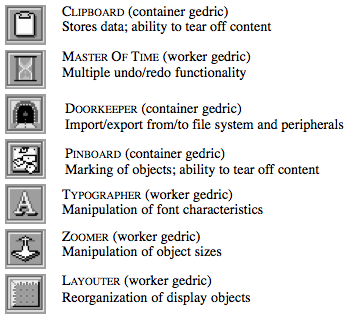
\includegraphics[width=.38\linewidth]{gfx/geisslerGedricIcons}} \quad
        \subfloat[Layouter Gesten.]
        {\label{fig:geisslerGedricIcons}%
         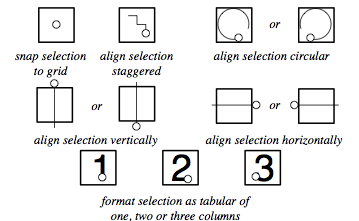
\includegraphics[width=.58\linewidth]{gfx/geisslerGedricLayouter}} \\
        \caption[Gedric \newline \citep{Geissler:1995}]{Beispiele für Gedric Icons (a) und Gesten einer Layoutfunktion (b).}\label{fig:geisslerGedric}
\end{figure}

\medskip Während Point \& Click Aktionen für Aufgaben zu Anwendungen, die üblicherweise mit der Maus ausgeführt werden, ausgelegt sind, raten Accot und Zhai zur \emph{Kreuzen}-Technik zur Stiftinteraktion \citep{Accot:2002}. Das experimentelle Zeichenprogramm \emph{CrossY}\index{CrossY} \citep{Apitz:2004} zeigt Interface Widgets\footnote{Widgets (dt. Steuerelemente) sind Interaktionselemente in einer grafischen Benutzeroberfläche (\ac{GUI}), beispielsweise eine Schaltfläche oder eine Bildlaufleiste.}, die Kreuzen erlauben. Um ein CrossY Button zu aktivieren, muss der Benutzer eine Linie von einer Seite des Buttons zur anderen zeichnen und somit den Button überqueren. Kreuzen macht es möglich, mehrere Aktionen in einer flüssigen Bewegung abzuhandeln. Zum Beispiel kann man die Farbe und Stärke der Electronic Ink des Stiftes gleichzeitig ändern, in dem man den Stift über benachbarte CrossY Widgets bewegt (siehe \autoref{fig:accotCrossY}).

\begin{figure}[bth]
	\begin{center}
	
	{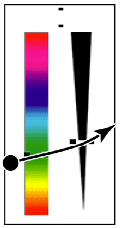
\includegraphics[width=0.28\linewidth]{gfx/accotCrossY}}
	\caption[CrossY \newline \citep{Johnson:2009}]{CrossY Interface Widgets erlauben Benutzer mehrere Parameter mit einer einzigen Bewegung zu ändern -- in diesem Beispiel die Stiftfarbe und -stärke.}
	\label{fig:accotCrossY}
	\end{center}
\end{figure}

\medskip So wie Skizzen mehrdeutig sein können, können auch stiftbasierte Interaktionen, wie das Drücken eines Buttons oder die Auswahl eines Menüpunktes, mehrdeutig sein. Wenn der Benutzer mit Hilfe des Stiftes, mit einem Objekt interagieren will, kann es sein, dass das System sein Ziel erst eindeutig machen muss. Zum Beispiel kann beim Drücken eines Buttons der Stift unabsichtlich zu einem anderen Button rutschen. Dieser Umstand wird auch \emph{Target Amibiguity}, oder laienhaft übersetzt \emph{Ziel Mehrdeutigkeit} genannt \citep{Mankoff:2000p77,Mankoff:2000}.

Eine Alternative, um gegen die Mehrdeutigkeit vorzugehen, ist, sie im Voraus zu bekämpfen. Pegasus und Chateau \citep{Igarashi:2001,Igarashi:2003} demonstrieren ein \emph{Empfehlungssystem}, das vorhersagt, was der Benutzer zeichnen wird und alle möglichen Aktionen aufzeigt. Diese Technik eignet sich besonders, wenn die Umgebung eine regelmäßige Grammatik aufweist oder strukturierte Eigenschaften wie Symmetrie genutzt werden soll.
Tsang et al. benutzten ein Empfehlungssystem in ihrem Programm, das Formen wie Flugzeugaußenhüllen modellieren kann \citep{Tsang:2004}. Das System bietet ein Overlay, das den Benutzer durch zusätzlichen Skizzierinput leitet. Benutzer zufolge führt dies zu präziseren Input. Das System benutzt die angefangenen Skizzen als Vorlagen, vergleicht diese mit Datenbankeinträgen um ähnliche Zeichnungen zu finden und empfielt zusätzliche Geometrie, die vielleicht dazu passen könnte.

\medskip Bae's 3D Kurvenmodellierungsystem zeigt wie verschiedene kaligraphische Interaktionstechniken zusammen benutzt werden können um eine flüssige Skizzierumgebung zu schaffen \citep{Bae:2008}. Das sog. \emph{ILoveSketch}\index{ILoveSketch} System imitiert ein physikalisches Skizzierbuch. Die Eingaben erfolgen per Stift und können optional durch Drücken von physikalischen Buttons durch die andere Hand verändert werden (siehe \autoref{fig:baeILoveSketch}). Das Interface verzichtet auf herkömmliche on-screen Buttons, Scrollbars und Menüs. Stattdessen gibt der Benutzer Kommandos durch Gesten, die oft vom Kontext abhängen. Zum Beispiel kann der Benutzer zu älteren Zeichnungen zurück >>blättern<<, in dem er an einer Ecke zieht. Um ein Objekt zu löschen, muss der Benutzer eine >>Durchstreichen<<-Geste anwenden. Viele Techniken in ILoveSketch betreffen Herausforderungen beim Skizzieren von 3D Objekten. Zum Beispiel errechnet das System automatisch aus der Arbeit des Benutzers die richtige Blickrichtung durch Drehungen und Verschiebungen.

\begin{figure}[bth]
	\begin{center}
	
	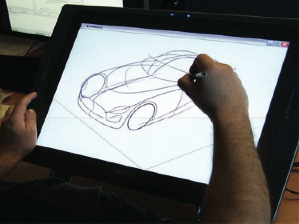
\includegraphics[width=0.7\linewidth]{gfx/baeILoveSketch}
	\caption[ILoveSketch \newline \citep{Johnson:2009}]{ILoveSketch zeigt ein >>natürliches<< Skizziersystem, welches mehrere kaligraphische Interaktionstechniken miteinander vereint \citep{Bae:2008}.}
	\label{fig:baeILoveSketch}
	\end{center}
\end{figure}

Alvarado fasste in \citep{Alvorado:2004} eine Liste aus sieben Designguidelines\index{Skizziersysteme!Designguidelines} zur Entwicklung von \emph{Sketch Recognition User Interfaces} (Benutzeroberflächen zur Skizzenerkennung), kurz SkRUIs zusammen: 

\begin{enumerate}
	\item Zeige Skizzenerkennungsergebnisse erst, wenn der Benutzer fertig ist mit dem Zeichnen
	\item Sorge für offensichtliche Hinweise, um das Skizzieren von der Erkennung zu unterscheiden
	\item Beschränke die Erkennung auf einen einzelnen Bereich, solange keine automatische Bereichserkennung machbar ist
	\item Integriere stiftbasiertes Editieren
	\item Skizzieren und Editieren sollten bestimmten Stiftbewegungen zugrunde liegen
	\item SkRUIs benötigen große Buttons
	\item Der Stift muss stets in real-time reagieren.
\end{enumerate}

Während WIMP Interfaces seit Mitte der 1980er Jahre weit verbreitet benutzt werden, müssen stiftbasierte Interfaces erst Fuß fassen. Um bessere Interaktionsrichtlinien, Interface Design Patterns und Toolkits zu entwickeln, muss die Forschung weiterhin Skizzierapplikationen entwickeln und evaluieren.

\subsection{Das Modusproblem}\label{sec:ModusProblem} \index{Modus} \index{Modus!- problem}
Oft interpretiert das User Interface Eingaben unterschiedlich, je nach dem in welchen Modus sich das Programm gerade befindet. Zum Beispiel hat ein Zeichenprogramm Eingabemodi wie \emph{Auswahl}, \emph{Linie zeichnen} oder \emph{Füllwerkzeug}. So ein Programm erlaubt dem Benutzer beispielsweise rechteckige Bereiche zu selektieren oder, wenn das Stifttool ausgewählt ist, zu zeichnen - beides indem der Benutzer eine Maustaste drückt und die Maus bewegt. Das Programm interpretiert die Eingaben hinsichtlich dem ausgewählten Werkzeug. 

Manchmal ist sich der Benutzer jedoch nicht im Klaren, in welchen Modus er sich befindet oder weiß nicht, wie er in einen anderen Modus umschalten kann. \graffito{Mehrere Programmmodi führen oft zu kognitiver Überlastung.} Die Handhabung der Modi führt oft zu kognitiver Überlastung der Benutzer, da sich diese auf das ausgewählte Tool konzentrieren, anstatt auf ihre Arbeit. Dabei spricht man auch vom sog. \emph{Modusproblem} \citep{Tesler:1981}, welches seit den Anfängen interaktiver Systemen besteht und nicht nur auf Skizziersoftware beschränkt ist.

\medskip \emph{Sketchpad}\index{Sketchpad}\footnote{Sketchpad war ein interaktives Designsystem aus dem Jahr 1963, das Technikern erlaubte Modelle mit Hilfe eines Lichtstiftes auf einem Display zu erstellen. Der Benutzer konnte dabei verschiedene Bedingungen (wie z.B. >>erstelle eine Linie parallel zu dieser Linie und erhalte das Verhältnis) auf das Gezeichnete anwenden. \citep{Sutherland:1964}}, das wohl erste nennenswerte elektronische Skizziersystem, behalf sich mit physikalischen Steuerelementen (Knöpfe, Schalter, Regler), durch die der Benutzer mit seiner linken Hand zu den verschiedenen Modi schalten konnte (siehe \autoref{fig:ellisSketchpad}) \citep{Sutherland:1964}. 

\begin{figure}[bth]
	{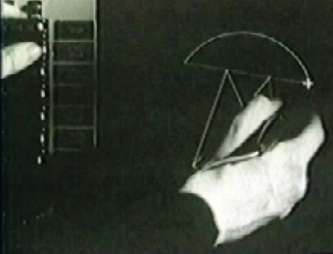
\includegraphics[width=\linewidth]{gfx/ellisSketchpad}}
	\caption[Sketchpad \newline \citep{Johnson:2009}]{Sketchpad unterstützt Benutzer beim Erstellen von Designzeichnungen mittels Stift (rechte Hand) und verschiedener Modi/Bedingungen (erreichbar über die Knöpfe auf der linken Seite).}
	\label{fig:ellisSketchpad}
\end{figure}

\begin{figure}
        \myfloatalign
        \subfloat[Input]
        {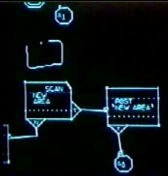
\includegraphics[width=.48\linewidth]{gfx/ellisGRAILinput}} \quad
        \subfloat[Output]
        {\label{fig:ellisGRAILinput}%
         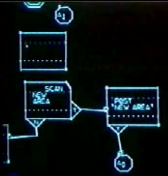
\includegraphics[width=.48\linewidth]{gfx/ellisGRAILoutput}} \\
        \caption[GRAIL Funktionalität \newline \citep{Johnson:2009}]{GRAIL analysiert die Benutzereingaben (a) und errechnet automatisch die bestimmungsgemäße Information (b) - hier z.B. ein Rechteck.}\label{fig:ellisGRAILoutput}
\end{figure}

\medskip Im \emph{GRAIL}\index{GRAIL}\footnote{RAND's GRAIL (GRAphical Input Language) System aus dem Jahr 1968, interpretierte Stifteingaben in einer besonderen visuellen Programmiersprache, um Flussdiagramme zu erstellen \citep{Ellis:1969}. Benutzer konnten via Eingabetablet semantisch wertvolle Modelldaten (Rechtecke, Pfeile, Schrift) und Kommandos (Lösche eine Linie, Bewege ein Rechteck, etc.) zeichnen und GRAIL errechnete anschließend automatisch die bestimmungsgemäße Information.} System können Benutzer nicht explizit in einen anderen Modus wechseln, um Text und Grafiken zu bearbeiten. Stattdessen versucht das System die Absichten des Benutzers aus einer Analyse des Gezeichneten bzw. dessen Kontext zu erschließen (siehe \autoref{fig:ellisGRAILoutput}) \citep{Ellis:1969}. 

\medskip Diese zwei früh entwickelten Systeme stellen zwei Extreme gegenüber, die zeigen, wie man mit dem Modusproblem umgehen kann. Sketchpad's Ansatz baut auf explizite Modiwechsel abseits des Stiftes auf, GRAIL's Ansatz auf implizite Modiwechsel, errechnet durch Stifteingaben.

\medskip Es scheint keinen >>richtigen<< Weg geben, um dem Modusproblem entgegenzuwirken. Implizite Modiwechsel scheinen natürlicher, aber nur wenn das System die Benutzereingaben richtig interpretiert. Interpretationstechniken sind fehleranfällig. Viele Systeme ermöglichen deswegen eine Kombination dieser zwei Arten oder verhängen Zeichenkonventionen.

\medskip Saund and Lank erforschten automatische Interpretationen und Modiwechsel, basierend auf Eingaben von Benutzern und bereits Gezeichneten \citep{Saund:2003p66}. Ihr \emph{Inferred-Mode Protocol} beschreibt einen Ansatz zur Analyse des Gezeichneten, um herauszufinden, ob Aktionen mit Absicht durchgeführt wurden oder nicht. War eine Aktion unklar, wird ein Mediator eingesetzt, der Methoden vorschlägt, um die Unklarheit zu beseitigen.

\medskip Li et al. verglichen in \citep{Li:2005} verschiedene Moduswechseltechniken\index{Modus!- wechseltechniken} für stiftbasierende User Interfaces. Dabei wurden folgende Techniken miteinbezogen: 
\begin{itemize}
	\item Tasten am Stift,
	\item Drücken und Halten,
	\item Benutzung der schwachen Hand, um einen physikalischen Button zu drücken,
	\item ein neue durckbasierte Methode und
	\item Benutzung des >>Radierers<< des Stiftes
\end{itemize}

Interessanterweise \graffito{Explizite Modiwechsel durch physikalische Buttons sind die schnellsten, am Fehler unanfälligsten und beliebtesten.}war die Methode, in der die schwache Hand verwendet wurde, die schnellste, am Fehler unanfälligsten und die beliebteste. Die >>Drücken und Halten<< Methode, wurde auch von Schilit et al. \citep{Schilit:1998} verwendet, die dies auch >>Rast<<-Geste bezeichneten. Microsoft Windows for Tablet PCs benutzt diese Geste beispielsweise, um die Rechtsklick-Kontextmenüs aufzurufen.

\medskip Bei Skizziersystemen tritt das Modusproblem vorwiegend auf, da es mehrere Typen an Stifteingaben gibt. Manche Eingaben sollen auf einer Seite angezeigt werden, da sie Wörter, Zeichnungen oder andere Modellelemente (\emph{Model Operations}) darstellen. Andere sollen im Hintergrund weiterverarbeitet werden, da sie Selektionen oder Kommandos (\emph{Environment Operations}) angeben.

\medskip \emph{Flow Selection}\index{Flow Selection} \citep{Johnson:2006} erlaubt Benutzern mit Hilfe der Rast-Geste nahtlos vom Zeichen- zum Selektionsmodus zu wechseln. Anschließende Operationen, wie Verschieben eines Teilabschnitts einer Linie, werden durch Bewegung des Stiftes ausgeführt, ohne den Stift vorher abzusetzen. Wieviel Einzelpunkte vom darunter liegenden Objekt selektiert werden - man spricht dabei auch von der Selektionstärke - hängt vom Abstand zur Stiftposition ab und wie lange der Benutzer den Stift an der selben Stelle ruhen lässt. Die Selektionstärek wird bei Operationen wie Verschieben oder Glättung verwendet (vgl. \autoref{fig:johnsonFlowSelection3}).

\begin{figure}
        \myfloatalign
        \subfloat[ ]
        {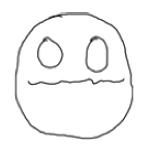
\includegraphics[width=.22\linewidth]{gfx/johnsonFlowSelection1}} \quad
        \subfloat[ ]
        {\label{fig:johnsonFlowSelection1}%
         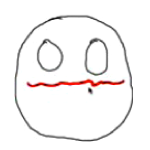
\includegraphics[width=.22\linewidth]{gfx/johnsonFlowSelection2}} \quad
		\subfloat[ ]
        {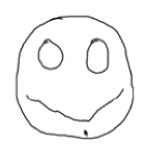
\includegraphics[width=.22\linewidth]{gfx/johnsonFlowSelection3}} \quad
        \subfloat[ ]
        {\label{fig:johnsonFlowSelection2}%
         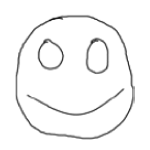
\includegraphics[width=.22\linewidth]{gfx/johnsonFlowSelection4}} \quad
        \caption[Modiwechsel \newline \citep{Johnson:2009}]{Modiwechsel der Flow Selection geschehen durch Halten und Bewegen des Stiftes \citep{Johnson:2006}. Der Benutzer positioniert dazu den Stift am gewünschten Objekt (a), bewegt es (b) ohne dabei den Stift zu heben (c). Der Benutzer hält den Stift anschließend an der Position bis die Kurve geglättet wurde (d) bevor er den Prozess durch heben des Stiftes abschließt.}\label{fig:johnsonFlowSelection3}
\end{figure}
\clearpage
\section{Die Bedeutung von Gestik}\label{sec:Gestik}\index{Gestik}

\begin{quote}
	\begin{flushright}{\slshape    
	    Design is an “activity of the mind \ldots grounded in mechanisms that evolved for interaction with the environment”.} \\ \medskip
	    --- \defcitealias{Wilson:2002}{M. Wilson}\citetalias{Wilson:2002} \citep{Wilson:2002}
	\end{flushright}
\end{quote}

Die Kombination von Gesten und Sprache bilden die Grundlage zur menschlichen dialogorientierten Interaktion. Sie sind sie somit auch ein wichtiger Bestandteil von Design (vgl. obiges Zitat von Wilson). Um diese Modalitäten auch richtig in \ac{HCI} anwenden zu können, man ihre Wechselwirkung zur Kommunikation verstehen.

\medskip Was sind eigentlich Gesten? Wenn ein Student mit einer Krawatte in die Klasse kommt und der Professor keine trägt, geben beide eine Aussage über ihre Einstellung zu der Klasse ab. 

Solche Handlungen nennt man auch >>Nonverbale Kommunikation<<. Ein breites Spektrum an Verhaltensweisen zählt dazu: die Wohn- und Arbeitsumgebungen, die wir schaffen; den Abstand, den wir zwischen uns und unseren Gegenüber einnehmen; ob wir unseren Körper bewegen, Augenkontakt herstellen, oder unsere Stimme erheben; all dies spielt zusammen und sendet Signale aus.

Die traditionelle Sicht auf Kommunikation teilt sich in die verbale und nonverbale Komponente bzw. ihr Zusammenspiel. Adam Kendon (1980) war einer der ersten, der sich mit dieser Ansicht beschäftigte. Er behauptet, dass sich mindestens eine Form des nonverbalen Verhaltens - Gestik - von einer Konverstation nicht trennen lässt. David McNeill zeigte 1992 in seinen bahnbrechenden Studien über Gestik und Sprache, dass Handbewegungen, die wir beim Sprechen produzieren, fest mit dem Gesprochenen, bezüglich Timing, Bedeutung und Funktion verstrickt sind. Wenn man Gestik ignoriert, ignoriert man einen Teil der Konversation.

\medskip Gestik ist ein Begriff\index{Gestik!Begriff}, der für einen großen Bereich steht. Betrachtet man z.B. lediglich Handbewegungen, kann man nicht einmal von einer eigenen Kategorie sprechen. \citep{Goldin:2003} 

Ekman und Friesen veröffentlichten 1969 einen Entwurf um nonverbales Verhalten zu klassifizieren und identifizierten dabei fünf Typen:
\begin{itemize}
	\item \emph{Illustratoren}, dies sind Verhaltensweisen, die das Gesagte untermalen, illustrieren oder verdeutlichen;
	\item \emph{Adaptoren}, dies sind Verhaltensweisen, die der Erregungsabfuhr oder der Selbststimulierung dienen können;
	\item \emph{Emblemen}, dies sind Verhaltensweisen, die das gesprochene Wort ersetzen;
	\item \emph{Regulatoren}, dies sind Verhaltensweien, die Interaktion steuern;
	\item \emph{Affektdarstellungen}, dies sind Verhaltensweisen, die Affekte, Stimmungen und Emotionen ausdrücken.
\end{itemize} \begin{flushright} \citep{Schaefer:2003} \end{flushright}

\index{Gestik!Handgesten}Im folgenden wird eine dieser fünf betrachtet: Illustratoren, auch \emph{Gestikulation} von Kendon (1980) und \emph{Gestik} von McNeill (1992) genannt. All diese Begriffe beschreiben Handbewegungen, die im direkten Bezug zu Gesprochenen stehen. Diese können das Tempo einer Rede vorgeben, auf Referenten verweisen, oder symbolischen Charakter haben, um den Inhalt einer Rede zu verdeutlichen. \citep{Goldin:2003}

\medskip Bezüglich Skizzen ermöglicht es Gestik, Meetingteilnehmer Details zu Zeichnungen zu erklären und zu interpretieren. Zusätzlich können hypothetische Modifikationen vorgenommen werden. Gestik bietet einen Mechanismus um Aktivitäten, Größen, Verbindungen, Richtungen oder Blickrichtungen zu kommunizieren. 

Dantec schildert in \citep{Dantec:2009} die Erfahrungen, die er in einem Architekturdesignmeeting mit Gestik gemacht hat. \graffito{Gesten sind das primäre Mittel um Designprobleme zu lösen.} Über das gesamte Meeting hinweg waren Gesten das primäre Mittel um Designprobleme zu lösen. Trotz der unbeständigen Natur von Gesten, wurden sie wiederholt und effektiv eingesetzt um komplexe Konzepte zu kommunizieren, ohne zuvor ein spezielles Training absolviert zu haben. Die Effektivität von Gesten und die Art, wie sie zwischen allen Teilnehmer fungierten, zeigte wie mehrere Teilnehmer mit eigenen Spezialisierungen ein verständliches Kommunikationsmittel fanden und so zum gemeinsamen Design beitrugen.

\medskip In Dantecs beschriebenen Szenario wurden Gesten auch dazu verwendet, um über Merkmale von Designs zu sprechen, die im zweidimensionalen Design nicht eindeutig hervorgingen. So machte z.B. ein Teilnehmer große schwungvolle Gesten, um die Form und Platzierung kleiner Fenster in einer Kapelle zu beschreiben (siehe \autoref{fig:dantecGestures}). Die Gesten zeigten mit der Hilfe von den Skizzen ein klares Bild von Form und Größe, boten zudem aber noch mehr. Sie beinhalteten eine metaphorische Qualität, da sie ausdrücken konnten, wie der Raum Ruhe erzeugt. Somit bekräftigten sie den Zweck des Gebäudes, der als Ort der Trauer gilt (siehe \extref{ext:dantecGestures}). Die Tatsache, dass die Nutzung von Gesten, physikalische Eigenschaften und metaphorische Qualitäten beschreiben kann, bestätigen auch die Forschungsergebnisse von Casasanto und Lozano, die die Rolle von Gesten beim Erarbeiten von abstrakten Konzepten untersuchten \citep{Casasanto:2006}.

\medskip Obwohl Gesten typischerweise nicht als Medium gesehen werden, die Informationen speichern (da sie keine permanenten Spuren hinterlassen), fanden Tang \& Leifer in \citep{Tang:1988p279} einen Beweis, dass Gesten Informationen effektiv in Stücke zerteilen und ins Gedächtnis zurückrufen können - insbesondere dann, wenn die Gesten von anderen nachgeahmt oder schriftlich bzw. skizzenhaft zu Papier gebracht werden. In einer Designstudie beobachteten sie diesen Umstand. Durch Nachahmung einer Geste und dessen Benennung mit der Phrase >>slide and tap<<, blieb eine Idee in den Köpfen der Teilnehmer verankert.

\medskip In der selben Studie wurden diese und auch andere Funktionen von Gesten beobachtet und statistisch erfasst. Die gerade erwähnte Funktion \emph{Speichern von Information} wurde einmal verzeichnet, das \emph{Verdeutlichen von Ideen} 24 mal, \emph{Hinweisen auf Ideen} neun mal und \emph{Aufmerksamkeit erlangen} 46 mal (vgl. \autoref{fig:tangStatistik}). Wie man durch die Statistik erkennen kann, spielen Gesten eine wichtige Rolle in kollaborativen Situationen, da sie hauptsächlich dazu benutzt werden, um anderen Personen Aktionen zu demonstrieren und die Aufmerksamkeit auf bestimmte Orte zu lenken.

\medskip \index{VideoDraw} Tang \& Minneman konzentrierten sich in \citep{Tang:1991p28} auf die Benutzung von Handgesten in Verbindung mit Zeichnungen. Handgesten treten oft in Verbindung mit Skizzen auf, um Informationen zu verdeutlichen. Aus diesem Grund entwickelten sie VideoDraw, ein kollaboratives Skizziersystem, das das Zusammenspiel von Skizzen und Gesten unterstützt. Das VideoDraw Setup besteht aus zwei Videokameras, die die Arbeitsflächen der Teilnehmer aufnimmt und direkt an den jeweilig gegenüberliegenden Bildschirm überträgt (vgl. \autoref{fig:tangVideoDraw}). Die Bildschirme fungieren als Whiteboard, auf das jeder Teilnehmer direkt mit Marker zeichnen kann. Die Zeichnungen \emph{und} Handgesten der Teilnehmer werden somit durch die Kamera erfasst und zum anderen Teilnehmer übertragen.

\medskip Handgesten können in VideoDraw beispielsweise eingesetzt werden, um einem Teilnehmer die geplante Bedienung eines User Interfaces zu erklären. Die Effektivität dieser Art von Gesten hängt von der Aufrechterhaltung der Verbindung zwischen den Händen und den Skizzen am VideoDraw Screen ab.

\medskip
\begin{figure}[bth]
	{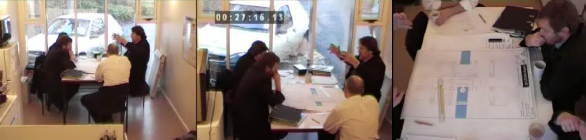
\includegraphics[width=\linewidth]{gfx/dantecGestures}}
	\caption[Beispiel von Gestik in einem Designmeeting. \citep{Dantec:2009}]{Ein Teilnehmer gestikuliert um Gebäudemerkmale zu beschreiben.}
	\label{fig:dantecGestures}
\end{figure}

\begin{extract}[Transkript eines Designmeetings. Skizzen und Gestik dienen als Ausdrucksmittel.]{
		\myfloatalign
		\begin{tabularx}{\textwidth}{p{1cm}X}
    		Adam & that wasn’t the idea I was anticipating that the hearses would be parked here [sketches] \\
			Anna & were there OK that’s fine yeah \\
			Adam & exactly as they are at the moment that the coffin would be drawn out	here and they would simply [points] walk it in I wasn’t thinking that they’d try and park \\
			Anna & no that’s OK \\
			Adam & in there \\
			Anna & yes well that’s what they’re wondering how that would work then so we’d work I wasn’t quite aware \\
			Adam & we’d work it exactly the same way as the present system I mean maybe this should be made more obvious by perhaps a different colour in the paving or something [sketches] I mean what I’m trying to say here is that that’s the vehicular line [sketches] \\
			Anna & yes \\
			Adam & and that these areas [points] are for people to mill about in and you’ve got a place for people to stand \\
			Anna & yes they will probably want to know how [points] how + how far that is from the because they’re going to be possibly carry the coffins in and most of the men are sort of in their seventies and eighties [laughs] carrying the coffin \\
		\end{tabularx}
	}
	\label{ext:dantecGestures}
	\captionX{Gestik in Designmeetings.}
\end{extract}

\begin{figure}[bth]
	{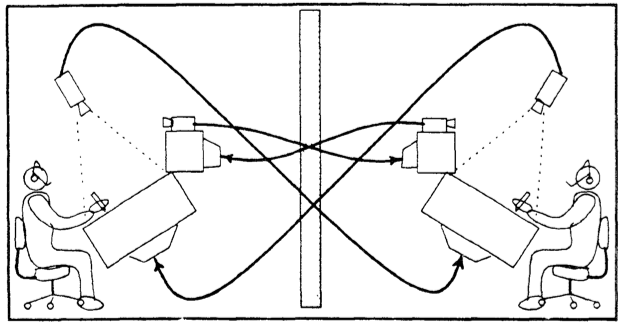
\includegraphics[width=\linewidth]{gfx/tangVideoDraw}}
	\caption[VideoDraw \newline \citep{Tang:1991p28}]{Schematische Darstellung von VideoDraw in einem Zwei-Personen-Szenario an verschiedenen Orten.}
	\label{fig:tangVideoDraw}
\end{figure}

%instead of newpage use \\[4cm]
\newpage Zusätzlich übermittelt VideoDraw auch Gesten mehrerer Hände und/oder Finger. Diese Kommunikation der Gesten ist reichhaltiger als die der meisten Computersysteme (typischerweise stellen diese lediglich einen mausgesteuerten Cursor zu Verfügung). VideoDraw überträgt ebenso das Gefühl von Dreidimensionalität.
Benutzer verfügen über >>räumliche<< Gesten und können sogar alltägliche Gegenstände ins Kamerabild holen, wodurch eine dreidimensionale Wahrnehmung von Raumverhältnissen den anderen Teilnehmern vermittelt werden kann.

\medskip Durch Observationen von Tang \& Minnemans System lassen sich vier Hauptmerkmale zusammenfassen.

\medskip VideoDraw:
\begin{itemize}
	\item übermittelt Handgesten unter den Teilnehmern,
	\item verursacht keine problematischen Verzögerungen in der Interaktion,
	\item bietet eine neuartige Wahrnehmung von räumlichen Beziehungen zwischen den Teilnehmern und ihrer Zeichenoberfläche und
	\item erlaubt mehreren Teilnehmern gleichzeitiges Arbeiten auf der gleichen Arbeitsfläche.
\end{itemize}

VideoDraw erlaubt Teilnehmern gewohnte Tätigkeiten auf eine neue Art zu erleben. Es ermöglicht Benutzern ihre Zeichenoberfläche mit anderen Teilnehmern am selben oder an einem anderen Ort zu teilen - ohne dass dabei Verwirrungen in der Interaktion entstehen. Es ermöglicht zudem die Hände der Teilnehmer näher aneinander zubringen, als es in der Realität je möglich wäre, ohne die Teilnehmer gegenseitig zu behindern. \citep{Tang:1991p28}
\clearpage
\section{Case Study - Digital and Paper Media}

2010 führten Hinckley et al. eine Studie durch, in der sie mittels Observationen herausfinden wollten, wie Personen mit Papier, Stiften und Hilfsmittel arbeiten. Sie stellten den Probanden die Aufgabe, Ideen zu einem hypothetischen Kurzfilm zu illustrieren. Zur Verfügung standen ihnen Notizblöcke, Scheren, Stifte, Klebeband und 20 Seiten an inspirierendem Material. Acht Personen nahmen an der Studie teil und unterstützten so Hinchley et al. auf der Suche nach Verhaltensmustern in Sachen Gestik und Arbeitsplatzstrukturierung. Neun Verhaltensweisen (V\itshape 1\upshape-V\itshape 9\upshape) stachen besonders hervor:

\medskip \begin{enumerate}[V\itshape 1\upshape)]
	\item Teilnehmer klemmten den Stift zwischen die Finger der starken Hand, wenn sie vom Schreiben zum Schnipselverschieben wechselten (\hyperref[fig:hinckleyPaperNotebook]{Abbildung \ref*{fig:hinckleyPaperNotebook}a}).
	\item Teilnehmer hielten Schnipsel mit einem Finger der schwächeren Hand an einer Stelle (\hyperref[fig:hinckleyPaperNotebook]{Abbildung \ref*{fig:hinckleyPaperNotebook}a}).
	\item Teilnehmer tendierten dazu, Schnipsel mit der schwächeren Hand festzuhalten, wenn sie darauf schrieben (\hyperref[fig:hinckleyPaperNotebook]{Abbildung \ref*{fig:hinckleyPaperNotebook}b}).
	\item Eine häufig eingesetzter Handgriff war das Halten eines Schnipsels mit Daumen und Zeigefinger während dem Schreiben (\hyperref[fig:hinckleyPaperNotebook]{Abbildung \ref*{fig:hinckleyPaperNotebook}b}).
	\item Teilnehmer benutzten nur Teile des inspirierenden Materials. Sie schnitten Schnipsel über dem Notizblock indem sie das Material mit der schwächeren Hand hielten und die stärke Hand zuschnitt (\hyperref[fig:hinckleyPaperNotebook]{Abbildung \ref*{fig:hinckleyPaperNotebook}c}).
	\item Teilnehmer schoben das Notizbuch nahe zu ihrem Körper, wenn sie zu den darüber liegenden Hilfsmittel fassten (\hyperref[fig:hinckleyPaperNotebook]{Abbildung \ref*{fig:hinckleyPaperNotebook}d}).
	\item Das Anhäufen von Schnipsel war ein häufiges Verhalten. Benutzer formten Stapel aus >>interessanten<< Objekten, während sie die übrigen in der schwächeren Hand hielten.
	\item Einige missbrauchten Schnipsel als Schablone, um einen Rahmen um ein Objekt zu zeichnen (\hyperref[fig:hinckleyPaperNotebook]{Abbildung \ref*{fig:hinckleyPaperNotebook}e}).
	\item Das Reißen von Papier war eine zweihändige Arbeit, die mit den Fingern vollzogen wurde (\hyperref[fig:hinckleyPaperNotebook]{Abbildung \ref*{fig:hinckleyPaperNotebook}f}).
\end{enumerate}

\begin{flushright} \citep{Hinckley:2010} \end{flushright}

\begin{figure}[bth]
	{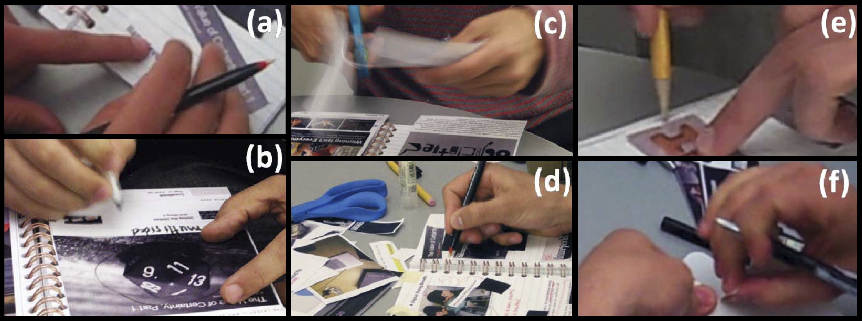
\includegraphics[width=\linewidth]{gfx/hinckleyPaperNotebook}}
	\caption[Designstudie über die Benutzung von Notizbüchern \newline \citep{Hinckley:2010}]{Verhaltensweisen bei der Benutzung von Notitzbüchern. \begin{inparaenum}[\itshape a\upshape)] \textbf{\item} Benutzer klemmen Stifte zwischen ihre finger, während sie Objekte bearbeiten. \textbf{\item} Daumen und Zeigefinger halten ein Objekt fest, während darauf geschrieben wird. \textbf{\item} Papierschnipsel fallen auf die Arbeitsfläche. \textbf{\item} Benutzer greifen oft nach Hilfsmitteln und neuen Inhalten, die über dem Notizbuch liegen. \textbf{\item} Zeichnen eines Rahmens mit einer Schablone, durch Halten der Schablone mit der Hilfshand und Nachfahren der Kanten mit dem Stift. \textbf{\item} Reißen einer Seite durch Festhalten des Papiers mit dem Daumen und Ziehen mit den Fingern der anderen Hand. Der Stift ist währenddessen wiederum zwischen den Fingern eingeklemmt. \end{inparaenum}}
	\label{fig:hinckleyPaperNotebook}
\end{figure}

Piper \& Hollan suchten im Weiteren den direkten Vergleich von Papier zu digitalen Medien und starteten dazu eine Untersuchung, in der sie Paare von Studenten mit Papier und digitalen Materialien auf Tabletop-Umgebungen arbeiten ließen. Die digitale Umgebung umfasste ein Tabletop-Display (vgl. \hyperref[fn:tableTop]{Fußnote \ref*{fn:tableTop}} in \autoref{sec:groupWareTools}) mit einer \emph{\ac{SDG}}\footnote{Single Display Groupware (\ac{SDG}) ist eine Spezialform von Groupware (vgl. \nameref{ch:CSCWDesign}) und beschreibt eine Displaytechnologie, die Eingaben von mehreren Benutzern gleichzeitig unterstützt \citep{Stewart:1997}. \ac{SDG}Ï führt zu höherem Engagement und gerechteren Aufgabenteilung \citep{Stewart:1999}.} - die andere enthielt Papier, Hilfsmittel und einen Tisch.

\medskip 20 Studenten einer neurowissenschaftlichen Einführungslehrveranstaltung nahmen fünf Wochen an der Untersuchung teil. Die Studenten mussten mit den vorgegebenen Systemen arbeiten und am Ende der Lehrveranstalung in der Lage sein, die Anatomie des Gehirnes aufzusagen, komplexe Systeme (wie z.B. die Entladung einer Nervenzelle) zu verstehen und zu beschreiben, sowie verschiedene Graphen und Schaltungen von Gehirnaktivitäten zu erstellen. Jede Teiluntersuchung umfasste folgende drei, vom Professor ausgewählte, Aktivitäten:
\begin{enumerate}
	\item das Beschriften der Gehirnanatomie,
	\item das Auseinandersetzen mit einem dynamischen System und
	\item das Zeichnen eines Graphen oder einer Schaltung.
\end{enumerate}
Das Ziel jeder Teiluntersuchung war, die Studenten auf ein kommendes Examen vorzubereiten. Die Arbeitsmittel beider Gruppen (analog, sowie digital Arbeitende) wurden soweit wie möglich angeglichen. Lediglich die Größe der Arbeitsfläche unterschied sich von der 79cm langen Bildschirmdiagonale zu den ca. 35cm Diagonale eines Blatt Papiers im A4 Format.

\medskip Papier- und Digitalmedien haben einzigartige und ergänzende Merkmale für kleine Lerngruppen. Die Studenten, die mit Papiermaterialen gearbeitet hatten, machten detaillierte Notizen und erarbeiteten meist ernsthaftere Arbeitsstrategien. Auf der anderen Seite diskutierten die Studenten, die am Tabletop-Display arbeiteten, ihre Ideen, bevor sie sich die Antworten ansahen, wiederholten Aktivitäten und schnitten besser im Endexamen ab. \citep{Piper:2009}

Während die folgenden Ergebnisse der Studie auf die Aktivitäten von Lerngruppen ausgelegt sind, können trotzdem auch allgemeine kognitive und soziale Merkmale in Bezug auf die Arbeit in beiden Welten (traditionell \& digital) entnommen werden.

\subsection{Kognitive Merkmale}
Papier ist das traditionelle Medium für Schulungsunterlagen. In Lerngruppen interagieren Studenten üblicherweise mit Papierdokumenten. Dadurch, dass die Teilnehmer der Studie keine vorgehende Erfahrung mit einem kollaborativen Tabletop Umgebungen hatten, hatten sie anfangs geringe Schwierigkeiten sich an das System zu gewöhnen. Jedoch förderte die Neuheit des digitalen Mediums einen gewissen Freiraum zur Interaktion. Munter kritzelten die Studenten mit den digitalen Stiften darauf los, während der Enthusiasmus bei den Studenten, die mit den traditionellen Mitteln arbeiteten sich in Grenzen hielt. Ebenso, ermutigten der geringe Aufwand und die geringen Konsequenzen (wenn etwas falsches gezeichnet wird, kann es leicht wieder gelöscht werden) die Studenten spontan Zeichnungen zu erstellen um die Diskussion zu unterstützen. 

Diese spontanen Skizzen können den Lernprozess ebenso in kognitiver Art unterstützen; die Skizzen bieten eine externe Abbildung der Diskussionen und bieten eine Grundlage um ein Verständnis zu entwickeln. Studenten, die mit Papierdokumenten arbeiteten, waren eher dazu geneigt die vorgegebenen Diagramme zu wenden, um auf der Rückseite zu zeichnen, anstatt direkt auf dem Bild. Die digitalen Medien ermutigten die Studenten nicht nur direkt auf ein Diagramm zu zeichnen, sondern auch die Radierfunktion öfter einzusetzen. Notizen auf Papierdokumenten wurden weniger ausradiert. Dadurch konnten die Studenten, die mit Papier arbeiteten, zurück gehen und ihre alten Notizen und Skizzen durchsehen, was bei den digitalen Materialien oft nicht mehr möglich war. Natürlich muss dies nicht zwangsweise so ablaufen. Die Formbarkeit digitaler Medien erlaubt zahlreiche interessante Lösungsansätze. Die Möglichkeit digitale Annotierungen zu löschen führt zu kognitiven Folgen, die nähere Untersuchungen benötigen.

\medskip Digitale Tische können ein dynamischeres und umfassenderes Erlebnis ermöglichen, als traditionelle Papierdokumente. Das hat positive wie negative Konsequenten. Studien über das Lernen mit Diagrammen zeigen, dass digital animierte Diagramme Personen dazu zwingen, das Diagramm wahrzunehmen, es richtig zuzuordnen und dann Diagrammänderungen durchzuführen, was zu einer höheren kognitiven Belastung führt, als statische Papierdiagramme \citep{Price:2002}. Andererseits ermöglichen große Touchscreens und interaktive Möglichkeiten, Formen an Interaktionen, die sich von den Papiermaterialen unterscheiden. Kognitionstheorien und die neuesten empirischen Forschungen zeigen, dass uns die körperliche Belastung hilft und zwingt abstrakte Konzepte zu verstehen \citep{Clark:1996,Johnson:1987,Nunez:1999,Varela:1991}. Das Zeichnen oder Nachverfolgen von Graphen mit dem Finger, ist ein konkreter kognitiver Prozess, der möglicherweise zu einem besseren Verständnis und Verinnerlichung eines abstrakten Konzeptes führt \citep{Goldin:2003}. \extref{ext:piperCognitiveAffordances} zeigt zwei Aussagen von Studenten, die mit digitalen Dokumenten arbeiteten. Piper \& Hollan glauben, dass konkrete Wahrnehmung eine zentrale Rolle im Verstehen kognitiver Askpekte im Zusammenhang mit Multitouchoberflächen spielen. \citep{Piper:2009}

\begin{extract}[Zwei typische Aussagen beim Arbeiten mit einem digitalen Tabletop-System.]{
		\myfloatalign
		\begin{tabularx}{\textwidth}{p{2cm}X}
    		Student D1 & Want to redraw it together to help memorize it? \\
			 & ... \\
			Student D2 & You want to try tracing it [the answer key]? It’s good practice. \\
		\end{tabularx}
	}
	\captionX{Arbeiten an digitalen Tabletop-Systemen.}
	\label{ext:piperCognitiveAffordances}
\end{extract}

\subsection{Soziale Merkmale}
Tabletop-Displays erlauben durch ihre Größe und ihre gemeinsame Nutzbarkeit, einen gleichmäßigen Zugang zu Materialen und erlauben gleichzeitiges Arbeiten. Aber verbessert dies den Lernprozess? Es gibt interessante Unterschiede zwischen den von Piper \& Hollan beobachteten parallelen Arbeitsweisen mit digitalen Dokumenten und seriellen Arbeitsweisen mit Papierdokumenten. Zum einen bedeutet paralleles Arbeiten, dass mehrere den gleichen und direkten Zugang zu Materialen haben. Zum anderen kann dies aber dazu führen, dass man wichtige Teile der Aktivitäten bzw. des Problemlösungsprozess verpasst. Eine serielle Arbeitsweise hat positive und negative Auswirkungen auf den Lernprozess. Während sich beide Studenten gemeinsam auf eine Aufgabe konzentrieren, macht einer den Hauptteil der Arbeit. Der Partner nimmt eine passive Rolle an.

\medskip Idealerweise würde die Lernumgebung Studenten dazu bewegen, sich gleichermaßen zu beteiligen und den Fokus auf die Aufgabe zu richten. Tabletop-Technologien erlauben Unterrichtenden zumindest die Darstellung der Lehrmittel soweit zu verändern, damit soziale Barrieren vermieden werden und eine ausgeglichene Beteiligung herrscht. \citep{Piper:2009}

\section*{Zusammenfassung}
Traditionelle und digitale Medien haben unterschiedliche Stärken und Schwächen. Papierdokumente sind billig, portabel und perfekt geeignet, um mit beiden Händen und einfachen Geräten, wie z.B. Stiften, daran zu arbeiten. Digitale Dokumente können hingegen mit Leichtigkeit editiert und schnell abgelegt bzw. abgerufen werden. Trotzdem kommt das Arbeiten mit einem strukturierten Softwaretool nicht an die Schnelligkeit von unstrukturierten Papier-und-Stift Skizzen heran.

Um auf Computer ähnlich gut skizzieren zu können, wurden Eingabegeräte wie Tablets geschaffen. Die Interaktion mit Tabletstiften unterscheidet sich jedoch stark von der der Maus. Aus diesem Grund wurden eigene Interaktionstechniken für stiftbasierte Skizziersysteme entwickelt. Skizziersysteme besitzen oft mehrere Programmmodi um die Funktion der Stifte zu bestimmen. Dabei kommt es oft zu kognitiven Überlastungen bei den Benutzern, welche mit Hilfe einiger Strategien vermieden werden sollten.

Gestik ist ebenso ein wichtiger Faktor im kollaborativen Designprozess und kann bei digitalen Arbeitsweisen berücksichtigt werden. Weitere Faktoren und Eigenschaften von kollaborativen computerbasierten Systemen werden nun im nächsten Kapitel erläutert.
% %*************************************************************
\chapter{Single- VS Groupdesign}\label{ch:SingleVSGroupDesign}
%*************************************************************

lorem ipsum

\section{was auch immer}

\begin{table}
    \myfloatalign
\begin{tabularx}{\textwidth}{p{5cm}X}
    \toprule
	    \tableheadline{Design Criteria} & \tableheadline{Reasons}
	     \\ \midrule
	\small{
    1) 
	Provide ways of conveying and supporting gestural communication.
	Gestures should be clearly visible, and should maintain their relation with objects within the work surface and with voice communication.} & \small{
	\begin{compactitem}
		%\setlength{\parskip}{-6pt}
		%\setlength{\topsep}{-6pt}
		%\setlength{\partopsep}{-6pt}
		\item gestures are a prominent action %\par
		\item gestures are typically made in relation to objects on the work surface %\par
		\item gestures must be seen if they are to be useful %\par
		\item gestures are often accompanied by verbal explanation 
	\end{compactitem} }
	\\ [-12pt] \hline
	\small{
    2) 
	Minimize the overhead encountered when storing information.} & \small{
	\begin{compactitem}
		\item only one person usually records information %\par
		\item other participants should not be blocked from continuing private or group work while information is being stored 
	\end{compactitem} }
	\\ [-12pt] \hline
	\small{
    3) 
	Convey the process of creating artifacts to express ideas.} & \small{ 
	\begin{compactitem}
		\item the process of creation is in itself a gesture that communicates information %\par
		\item speech is closely synchronized with the creation process %\par
		\item artifacts in themselves are often meaningless 
	\end{compactitem} }
	\\ [-12pt] \hline
	\small{
	4) 
	Allow seamless intermixing of work surface actions and functions} & \small{ 
	\begin{compactitem}
		\item a single action often combines aspects of listing, drawing and gesturing %\par
		\item writing and drawing alternates rapidly %\par
		\item actions often address several functions 
	\end{compactitem} }
	\\ [-12pt] \hline
	\small{
	5) 
	Enable all participants to share a common view of the work surface while providing simultaneous access and a sense of close proximity to it} & \small{ 
	\begin{compactitem}
		\item people do not see the same things when orientation differs %\par
		\item simultaneous activity is prevalent %\par
		\item close proximity to the work surface encourages simultaneous activity 
	\end{compactitem} }
	\\ [-12pt] \hline
	\small{
	6) 
	Facilitate the participants natural abilities to coordinate their collaborations} & \small{ 
	\begin{compactitem}
		\item people are skilled at coordinating communication %\par
		\item we do not understand the coordinating process well enough to mechanize it 
	\end{compactitem} }
	\\ [-12pt] \bottomrule
\end{tabularx}
  \caption[Tangs Designkriterien]{Tangs Designkriterien zur Erstellung von Multi-User Zeichenprogrammen.}
  \label{tab:tangDesignKriterien}
\end{table}
 % Single- VS. Groupdesign
%*************************************************************
\chapter{CSCW \& Groupware}\label{ch:CSCWDesign} \index{CSCW}
%*************************************************************

	Der Begriff >>Computer Supported Cooperative Work<< (\ac{CSCW}) bezeichnet ein multidisziplinäres Forschungsgebiet, das die kooperative Zusammenarbeit mehrerer Gruppen untersucht und Technologien zu ihrer Unterstützung entwickelt. \ac{CSCW} existiert seit den frühen achtziger Jahren. Um herauszufinden, wie die Technik Menschen bei ihrer Zusammenarbeit unterstützen kann, organisierten Irene Greif und Paul Cashman im Jahre 1984 einen Workshop für Personen, die sich mit der Arbeitsweise von Menschen auseinandersetzten \citep{Grudin:1994}. Unter diesen Personen befanden sich Spezialisten aus verschiedenen wissenschaftlichen Bereichen, wie zum Beispiel Ökonomie, Sozialpsychologie, Anthropologie, Ethnologie und Pädagogik. Dieser Workshop war der Versuch der Techniker, Teamarbeit besser zu verstehen und folglich unterstützende Technologien entwickeln zu können \citep{Grudin:1994, Rama:2006p245}. Seither hat \ac{CSCW} sich zu einem nahezu riesigen wissenschaftlichen Forschungsgebiet entwickelt, dem sich heute unzählige Experten widmen. Trotzdem sind sich die Wissenschaftler nicht immer ganz einig bei der Definition des Begriffes \ac{CSCW}. Die Bedeutung von >>Cooperative Work<< erscheint nicht eindeutig und führt häufig zu unterschiedlichen Interpretation seitens wissenschaftlicher Autoren \citep{Gerlicher:2007p241}. Einige setzen >>Cooperation<< gleich mit >>Collaboration<<, andere hingegen unterscheiden die beiden Begriffe sehr strikt. Dillenbourg et al. definieren die Begriffe beispielsweise so: 
	
	\medskip\begin{quote}{>>Cooperation and collaboration do not differ in terms of whether or not the task is distributed, but by virtue of the way in which it is divided; in cooperation the task is split (hierarchically) into independent subtasks; in collaboration cognitive processes may be (heterarchically) divided into intertwined layers. In cooperation, coordination is only required when assembling partial results, while collaboration is “...„ a coordinated, synchronous activity that is the result of a continued attempt to construct and maintain a shared conception of a problem.<<} \begin{flushright}\citep{Dillenbourg:1995} \end{flushright}\end{quote}
	
	\medskip Die beiden Begriffe unterscheiden sich also nicht darin, \emph{ob} Arbeit auf mehrere Individuen aufgeteilt wird oder nicht, sondern in der Art und Weise, \emph{wie} sie aufgeteilt wird. Bei >>Cooperation<< wird die Arbeit in einzelne, unabhängige Module aufgeteilt, die zuerst abgewickelt und danach wieder zu einem Ganzen zusammengesetzt werden können. Koordination wird in diesem Fall hauptsächlich beim Zusammenfügen der Module benötigt. >>Collaboration<< hingegen ist eine koordinierte, synchrone Aktivität und resultiert aus dem fortwährenden Versuch, eine gemeinsame Auffassung eines Problems zu konstruieren und zu erhalten.
	
	In dieser Arbeit werden die beiden Begriffe synonym verwendet, da sich beide aus dem Englischen als >>Zusammenarbeit<< übersetzen lassen. Um den Begriff \ac{CSCW} jedoch besser zu verstehen, sollen weitere Definitionen von >>Cooperative Work<< begutachtet werden.
	
	Die Ökonomie kennt den Begriff >>Cooperative Work<< schon sehr lange und Marx definiert ihn als mehrere Individuen, die gemeinsam in einer koordinierten Art und Weise an einem oder mehreren, zusammengehörigen Produktionsprozessen arbeiten \citep{Marx:1867}. Im deutschen Sprachraum wurde diese Definition im 19. Jahrhundert häufig durch andere Autoren wiederverwendet, jedoch gibt es sehr viele Formen von >>Cooperative Work<< und es gibt in der Literatur keine klare Trennung zwischen Begriffen wie >>Cooperative Work<<, >>Collaborative Work<<, >>Collective Work<< und >>Group Work<< \citep{Bannon:1990p244}.
	
	Die Definition von >>Cooperative Work<< nach Bannon und Schmidt besagt, dass sie im Allgemeinen aus Arbeitsprozessen besteht, die ein Produkt oder ein Service hervorbringen. Ein typisches Merkmal dieser Arbeitsform ist die Planung der Abwicklung, die vor Beginn der eigentlichen Arbeit durchgeführt wird. >>Cooperative Work<< beinhaltet \emph{direkte}, \emph{indirekte}, \emph{verteilte} und \emph{kollektive} Arten der Interaktion. \emph{Kollektiv} in einer Gruppe geleistete Arbeit, sprich >>Group Work<< ist lediglich eine spezielle Form von >>Cooperative Work<<. Es ist aber ebenfalls möglich, dass >>Cooperative Work<< von einer geographisch \emph{verteilten} Gruppe halb autonomer Personen geleistet wird, die bei der Abwicklung strategisch nach eigenem Ermessen vorgehen. Zusätzlich kann >>Cooperative Work<< \emph{indirekt}, über den Arbeitsprozess selbst, als auch \emph{direkt}, durch Kommunikation zwischen den einzelnen Gruppenmitgliedern durchgeführt werden. \citep{Bannon:1990p244}
	
	\bigskip Die Erkenntnisse, die bei der Erforschung von \ac{CSCW} gewonnen werden, verwendet man dazu, sinnvolle Groupware \index{Groupware} zu konzipieren. Groupware bezeichnet also die technische und praktische Umsetzung, die auf den Theorien der \ac{CSCW}-Forschung basiert. Alle Systeme, Applikationen und Werkzeuge, die \ac{CSCW} unterstützen, können somit unter dem Begriff Groupware zusammengefasst werden \citep{Koch2008, Gerlicher:2007p241}. Häufig werden diese Systeme auch als >>kollaborative Software<< bezeichnet \citep{Bannon:1990p244}. Gerlicher definiert Groupware wie folgt:
	
	\clearpage
	
	\medskip\begin{quote}>>Der Begriff Groupware bezeichnet ein aus Software und eventuell spezifischer Hardware bestehendes System, das die Zusammenarbeit im Team durch die Schaffung von Kommunikations- und/oder Koordinationslösungen unterstützt oder ermöglicht.<< \begin{flushright}\citep{Gerlicher:2007p241}\end{flushright}\end{quote}
	
	\medskip Michael Koch definiert Groupware als:
	
	\medskip\begin{quote}>>[...] Nevertheless, there are some technologies and tools [Groupware] that facilitate shaping [...] socio-technical systems. For these technologies and tools the term Groupware is used. In contrast to traditional computer systems that are primarily designed for a single user, the major goal of Groupware is to assist a group of users in communicating, in collaborating, and in coordinating their activities.<< \begin{flushright}\citep{Koch2008}\end{flushright}\end{quote}
	
	\medskip Groupware unterscheidet sich also von >>Ein-Benutzer-Systemen<< darin, dass sie für mehrere Benutzer konzipiert ist und versucht, die höchste Effizienz und Flexibilität für die Teamarbeit dieser Benutzer zu gewährleisten. Gerlicher nennt die folgenden Gründe, warum Groupware eingesetzt wird: 
	
	\begin{itemize}
		\item {Verbesserung der Kommunikation in der Gruppe}
		\item {Ermöglichen von Kommunikation, wo sie sonst nicht möglich wäre}
		\item {Ermöglichen von Telearbeit (für geographisch entfernte Benutzer)}
		\item {Einsparung von Reisekosten}
		\item {Bündelung von Fachwissen und Gedankenaustausch in der Gruppe}
		\item {Bildung von Gruppen mit gemeinschaftlichem Interesse}
		\item {Reduktion von zeitlichem und finanziellen Aufwand bei der Koordination von Gruppen}
		\item {Problemlösung in der Gruppe}
		\item {Erlangung neuer Kommunikationsmöglichkeiten, beispielsweise dem anonymen oder strukturierten Informationsaustausch}
	\end{itemize}
	\begin{flushright}
		\citep{Gerlicher:2007p241}
	\end{flushright}
	
	Demgegenüber steht die Schwierigkeit, erfolgreiche Groupware Systeme zu entwickeln. Im Gegensatz zu single-user Software ist dies äußerst komplex und es gibt viele kritische Faktoren. Zum einen sind die technischen Voraussetzungen diffiziler, weitaus entscheidender ist jedoch, dass Groupware von der Gruppe lebt und daher ist die Akzeptanz durch die Zielgruppe maßgebend für den Erfolg von Groupware \citep{Gerlicher:2007p241}.
	
	\medskip \ac{CSCW} soll aber nicht nur Technologien und Werkzeuge zur Unterstützung von Kollaboration bereitstellen, sondern auch soziotechnische Systeme entwickeln \citep{Koch2008}. In den 1950er Jahren wurden Experimente durchgeführt, bei denen technische Systeme in mehrere verschiedene soziale Gruppen eingeführt wurden. Dabei stellte man fest, dass die Technologieeinführung in den Gruppen sehr unterschiedliche Auswirkungen hatte. Dadurch kamen die Wissenschaftler zum Schluss, dass das technische, als auch das soziale System auf diese Zusammenführung hin optimiert werden müssen, um ein erfolgreich funktionierendes, einheitliches Gesamtsystem hervorzubringen \citep{Koch2008}. Wenn diese Optimierung nicht passiert und bei der Einführung der Technik die sozialen Aspekte und Eigenheiten nicht berücksichtigt werden, kann das Ergebnis nur suboptimal sein. Soziale Prozesse sind die Basis für die Entwicklung und das Design von neuen Technologien und Systemen und umgekehrt strukturieren diese Technologien die Möglichkeiten des sozialen Austauschs. Für den Erfolg von neuen Technologien ist es unerlässlich, diese sozialen und technischen Aspekte bei Entwicklung und Design mit einzubeziehen \citep{Mumford:2000}.
	
	Das Forschungsgebiet \ac{CSCW} versucht also soziale Interaktion in Gruppen und Teams zu verstehen und technische Systeme zur Unterstützung selbiger zu konzipieren, zu entwickeln und zu evaluieren \citep{Koch2008}.

\section{Klassifikation von CSCW} \index{CSCW!Klassifikation}

\ac{CSCW} kennt zwei Dimensionen: Raum und Zeit. Dies sind die Kriterien, nach denen \ac{CSCW} und Groupware eingeteilt werden. \autoref{fig:ramaCSCW} illustriert die Kategorisierung von \ac{CSCW} und ordnet den vier sich aus der Überschneidung der Dimensionen ergebenden, Quadranten einige Beispiele zu. 

Der erste Quadrant umfasst alle Systeme und Technologien, bei denen die Benutzer zur selben Zeit am selben Ort sein müssen. Beispielsweise könnten sich zwei Personen in einem Meetingraum treffen und gemeinsam Konzepte an einem digitalen Whiteboard ausarbeiten. Sie teilen zeitliche und räumliche Komponenten miteinander. 

\begin{figure}
	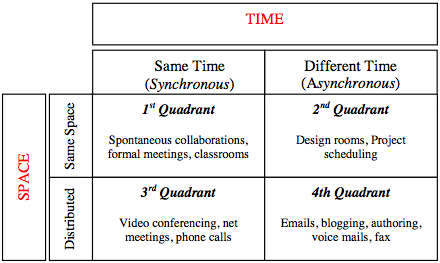
\includegraphics[width=\textwidth]{gfx/ramaCSCWQuadranten.png}
	\caption[CSCW-Kategorien \newline \citep{Rama:2006p245}]{Die Grafik illustriert die Unterteilung von CSCW in vier Kategorien, die sich durch ihre räumlichen und zeitlichen Eigenschaften unterscheiden. Der Faktor Zeit definiert, ob Zusammenarbeit in einer Gruppe synchron oder asynchron passiert und der Faktor Raum definiert, ob sie am selben oder an geographisch distanzierten Orten stattfindet.}
	\label{fig:ramaCSCW}
\end{figure}

Der zweite Quadrant kategorisiert all jene Technologien, die Personen am selben Ort zu unterschiedlichen Zeiten nutzen können. Ein Designraum mit elektronischen Geräten könnte ein Beispiel dafür sein. Angenommen, eine Person überlegt sich ein Konzept und zeichnet Skizzen auf ein Tabletop Display. Zu einem späteren Zeitpunkt, als die Person den Raum bereits verlassen hat, kommt eine andere Person herein, arbeitet mit den Skizzen weiter und entwickelt eigene Konzepte, die sie wiederum auf dem Tabletop festhält. 

Zum dritten Quadranten gehören alle Systeme, die zur selben Zeit an verschiedenen Orten eingesetzt werden können. Das wohl bekannteste dieser Systeme ist das Telefon. Es kann nur von zwei Personen gleichzeitig benutzt werden, aber die Personen können sich dazu an beliebigen Orten befinden.

Im vierten Quadranten befinden sich alle Technologien, die zu unterschiedlichen Zeiten an unterschiedlichen Orten zum Einsatz kommen. E-Mail, das elektronische Nachrichtensystem, ist ein gutes Beispiel solcher Groupware. Um auf diesem Wege zu kommunizieren, müssen zwei Personen weder gleichzeitig damit interagieren, noch sich am selben Ort befinden. 

\medskip Gerlicher definiert zusätzlich eine weitere Kategorie in \ac{CSCW}, auf die im Abschnitt \nameref{sec:multisynchronousCSCW} näher eingegangen werden soll, nachdem die vier grundlegenden Kategorien im folgenden näher definiert werden.

\subsection{Asynchrone Systeme} \index{CSCW!Asynchrone Systeme}

Unter asynchroner Groupware versteht man Systeme, die keine Echtzeitanforderungen erfüllen müssen. Das bedeutet, dass die Nutzung dieser Systeme im Normalfall zeitversetzt erfolgt. Die wohl bekannteste asynchrone Groupware-Anwendung ist die digitale Übermittlung von Textnachrichten in Form einer \emph{E-Mail}. Diese Nachrichten können an und von mehreren Personen versendet, empfangen und weitergeleitet werden. Dabei müssen Absender und Empfänger nicht gleichzeitig online sein, denn die \emph{E-Mail} kann zu jedem beliebigen Zeitpunkt vom Empfänger abgerufen werden.

Eine andere, jedoch der \emph{E-Mail} sehr ähnliche Form asynchroner Groupware, sind \emph{Newsgroups und Mailinglisten} \citep{Gerlicher:2007p241}. Sie dienen dem Nachrichtenaustausch in einer größeren Gruppe an Benutzern. \emph{Newsgroups} zeigen Nachrichten nur dann an, wenn ein Benutzer diese direkt anfordert, \emph{Mailinglisten} hingegen werden automatisch an all jene Personen weitergeleitet, welche die entsprechende Liste abonniert haben.

Auch \emph{Workflow-Management-Systeme} werden von Gerlicher \citep{Gerlicher:2007p241} zur asynchronen Groupware gezählt, da sie die Arbeit unterschiedlicher Personen in einer Organisation regeln. Sie dienen der Steuerung arbeitsteiliger Prozesse. Man bezeichnet sie auch als \emph{Geschäftsprozess-Management-Systeme}.

Das World Wide Web (WWW) ist ein \emph{Hypertext-basiertes System} und gehört ebenfalls zur asynchronen Groupware \citep{Gerlicher:2007p241}, da es einer sehr großen Anzahl an Personen ermöglicht, auf digitalem Wege Informationen auszutauschen. \emph{Hypertext-basierte Systeme} nutzen das Internet oder ein bestimmtes Intranet, um ihre Dienste über einen Webbrowser zugänglich zu machen. Solch eine Webschnittstelle kann prinzipiell für fast jede Art der asynchronen Groupware implementiert werden. 

Schlussendlich nennt Gerlicher noch \emph{Gruppenkalender} als asynchrones Groupware System. Der \emph{Gruppenkalender} ist ein Tool, das sehr häufig in größeren Unternehmen eingesetzt wird. Er ermöglicht die Terminplanung und Koordination von vielen Personen. Terminkonflikte werden automatisch erkannt und das System kann eigenständig jene Zeiträume finden, zu denen jeder erforderliche Teilnehmer eines Meetings frei zur Verfügung steht. Dies setzt jedoch eine gute Datenpflege aller Benutzer voraus und wird teilweise als unangenehmer Eingriff in die Privatsphäre empfunden \citep{Gerlicher:2007p241}.
\clearpage

\subsection{Synchrone Systeme} \index{CSCW!Synchrone Systeme}

Dem gegenüber stehen synchrone Groupware Systeme, die sich dadurch charakterisieren, dass Benutzer zeitgleich auf Daten und Informationen zugreifen \citep{Gerlicher:2007p241}. Ein Beispiel dafür sind \emph{elektronische Tafeln}, denn sie erlauben mehreren Nutzern, die sich an unterschiedlichen Orten befinden, auf eine für alle sichtbare Fläche zu zeichnen. Häufig werden solche Tafeln bei Besprechungen eingesetzt, bei denen die Teilnehmer nicht im selben Raum sind. Dadurch wird es möglich, Konzepte und Ideen besser zu kommunizieren und für die anderen greifbarer zu machen.

\emph{Application Sharing Systeme} zählen ebenfalls zur synchronen Groupware und gestatten das Teilen von Drittapplikationen mit anderen Personen \citep{Gerlicher:2007p241}. Man bezeichnet diese Anwendungen im Englischen auch als \emph{Remote Desktop}\footnote{Zu Deutsch: Entfernter Schreibtisch. Gemeint ist damit die virtuelle Schreibtischfläche des Betriebssystems.}. Dadurch wird es möglich, mit geografisch distanzierten Kollegen an jedem beliebigen Programm zu kooperieren. Beide Benutzer sehen die Applikation, die auf einem der Computer läuft und können mit ihr interagieren. 

Weitere synchrone Systeme sind \emph{Video- und Multimediale Konferenzsysteme} \citep{Gerlicher:2007p241}. Erstere übertragen Video und Audio an mehrere verteilte Computer und werden eingesetzt, um virtuelle Meetings abzuhalten. Die Teilnehmer befinden sich meist an verschiedenen Orten und können so fast genauso kommunizieren, als würden sie sich in einem Raum befinden. Letztere bieten zusätzlich die Möglichkeit, multimediale Inhalte (beispielsweise Präsentationen) an die Teilnehmer der Konferenz zu übertragen. Systeme zu Entscheidungsfindung sind oft ein integraler Bestandteil solcher Software und bieten Werkzeuge für Ideenfindung und Brainstorming. Über auf diesem Wege generierte Konzepte kann dann abgestimmt und so die Spreu vom Weizen getrennt werden. 

\emph{Chat-Systeme}, ebenfalls der synchronen Groupware zuzuordnen, sind weitgehend bekannt und werden sehr häufig eingesetzt. Benutzer können durch diese Anwendungen in Echtzeit untereinander Textnachrichten austauschen und so eine Konversation führen, als säßen sie sich gegenüber. 

\subsection{Multisynchrone Systeme}\label{sec:multisynchronousCSCW}\index{CSCW!Multisync. Systeme}

\emph{Versionsverwaltungssysteme} werden von Gerlicher als multisynchrone Systeme definiert \citep{Gerlicher:2007p241}. Häufig werden diese in Softwareprojekten und auch bei der Erstellung von umfangreichen Dokumenten, beispielsweise Büchern eingesetzt. Das System übernimmt die Verwaltung der Dateien und sichert die Konsistenz der Daten. Es wird dadurch möglich, dass mehrere Personen gleichzeitig an der selben Datei arbeiten. Tatsächlich haben aber alle Benutzer eine eigene Kopie der Datei und das System synchronisiert die Dateien im Nachhinein selbständig. Ein weiterer großer Vorteil von \emph{Versionsverwaltungssystemen} ist die Nachvollziehbarkeit von Änderungen \citep{Gerlicher:2007p241} an einzelnen Dateien. Das System legt für jede neue Version einer Datei ein Backup ab, das zu einem späteren Zeitpunkt bei Bedarf wiederhergestellt werden kann. Es ist zu jedem Zeitpunkt klar, wer welche Änderungen an einer bestimmten Datei durchgeführt hat. 

\bigskip Es wird deutlich, dass \ac{CSCW} und Groupware sehr weitläufig sind und viele verschiedene Bereiche betreffen. Daher ist es bis heute immer noch eine große Herausforderung geblieben, bedienbare, effiziente und intuitive Systeme zu entwickeln, die die Arbeit der Benutzer tatsächlich optimieren und keinen Mehraufwand verursachen. Der folgende Abschnitt widmet sich den Problemfeldern, die damit zusammenhängen.

\section{Design von Groupware} \index{Groupware!Design}

Eine formale Beschreibung von Groupware Lösungen zu geben ist äußerst schwierig, da sie stark von den Menschen bzw. den organisatorischen Umständen abhängen von und in denen sie eingesetzt werden \citep{Suchman:1995}. Obwohl also alle Groupware Systeme mit eigenen Anforderungen und Gegebenheiten zurecht kommen müssen, gehen Entwickler beim Design normalerweise von bekannten und bewährten Lösungen aus und versuchen dann, diese für die neue Situation anzupassen \citep{Herrmann:2003}. Diese Vorgehensweise ist natürlich völlig legitim, kann aber zu Schwierigkeiten führen wenn es nicht gelingt, die Expertise erfahrener Entwickler auf die Kollegen zu übertragen. Eine gute Dokumentation ist daher von großer Bedeutung, denn sie erlaubt es den Entscheidungsträgern im Projekt, schon sehr früh mit Endbenutzern über Funktionalität und Design zu diskutieren. Hermann et al. schlagen daher vor, sogenannte Patterns\index{Groupware!Patterns}\footnote{aus dem Englischen: >>Muster<< beschreiben zum einen ein Problem, das immer wieder in einer gegebenen Umgebung auftritt und bieten eine generische Lösung dafür. Diese Lösung muss so formuliert werden, dass sie jedes mal (nahezu) unverändert eingesetzt werden kann. \citep{Herrmann:2003}} zu verwenden \citep{Herrmann:2003}. 

\medskip Die Idee, Wissen und Problemlösungen in Form von Patterns zu archivieren, gibt es schon länger und Gamma et al. haben dieses Konzept der Patterns von urbaner Architektur auf Softwarearchitektur umgemünzt und eine Kollektion von Patterns für objektorientierte Softwareentwicklung veröffentlicht \citep{Gamma:1995}. Im Bereich \ac{HCI} bietet Jan Borchers einige gute Beispiele für User Interface Patterns \citep{Borchers:2000}.

\medskip Da Groupware stark abhängig vom Umfeld ist, müssen Patterns in dieser Domäne nicht nur technische, sondern auch soziale Aspekte berücksichtigen. Dazu gehören unter anderem soziale Unternehmensstrukturen, involvierte Personen und ihre Rollen im Unternehmen. Groupware Patterns sollten also anwendungsorientiert sein und dabei helfen, soziotechnische Systeme zu verstehen und zu designen \citep{Herrmann:2003, Eason:1988}. Laut Herrmann et al. bestehen Groupware Patterns aus statischen und dynamischen Aspekten. Statische Aspekte beschreiben die technische Struktur des Patterns und dynamische Aspekte repräsentieren die sozialen Prozesse, die involviert sein können. Da der dynamische Teil jedoch sehr variabel ist und schwer generalisiert werden kann, müssen und können Groupware Patterns nicht vollständig sein. Diese Unvollständigkeit wird bewusst beibehalten, damit menschliches Verhalten und menschliche Eigenheiten nicht als fix definiert angenommen werden. Diese Faktoren sind überaus instabil und müssen auch so behandelt werden \citep{Herrmann:2003}.

\medskip Für eine ausreichend vollständige und anschauliche Beschreibung von Groupware Patterns propagieren Herrmann et al. Fotos, Screenshots und Kurzvideos, die typische Situationen zeigen, in denen das jeweilige Pattern zum Einsatz kommt. Das technische System soll also in einem sozialen Kontext gezeigt werden, um Eigenheiten und Herausforderungen besser vermitteln zu können. Da Patterns häufig auf elektronischem Wege, beispielsweise im Internet oder auf digitalen Datenträgern veröffentlicht werden, ist eine multimediale Darstellung die beste Form der Veranschaulichung. Zusätzlich sollte es ein Diagramm geben, das eine formale und schematische Beschreibung des Lösungsansatzes bietet. Gegenüber normalen Textbeschreibungen haben Diagramme den Vorteil, dass sie einprägsamer und leichter wiedererkennbar sind. Außerdem können sie auf verschiedene Arten gelesen werden und sind daher flexibler. Es müssen also Repräsentationen der Patterns geschaffen werden, die eine ausreichend detaillierte Beschreibung von Problem und Lösung bieten und gleichzeitig jedoch genügend Freiräume und Flexibilität beibehalten, um die menschlichen Faktoren nicht von vornherein zu stark einzuschränken. Bei der Verwendung von Groupware Patterns muss man sich jedoch im Klaren darüber sein, dass das Verhalten und die Eigenheiten der Benutzer von soziotechnischen Systemen niemals konkret vorausgesagt bzw. angenommen werden können und somit Patterns keine allumfassende, immer gültige Lösung, sondern nur einen Ansatz darstellen, der sich unter gewissen Bedingungen erfolgreich bewährt hat \citep{Herrmann:2003}.

\bigskip Ein Begriff, der in den Fachbereichen \ac{CSCW} und \ac{HCI} sehr häufig vorkommt ist >>Awareness<<.\index{Awareness} Er bezeichnet das Bewusstsein eines Benutzers über die momentanen Aktivitäten und Zustände der anderen Benutzer \citep{Dourish:1992, Hornecker:2008}. Bei Groupware, die den Benutzern ermöglicht, gleichzeitig in der selben Arbeitsumgebung zu arbeiten, ist Awareness ein äußerst wichtiges Kriterium für eine hohe Usability. Die Zusammenarbeit der Personen kann nur dann ausreichend zufriedenstellend sein, wenn jeder immer über die anderen Bescheid weiß. Ohne diese Information wäre es gar nicht oder nur schwer möglich, die folgenden kollaborativen Aktivitäten durchzuführen:

\begin{itemize}
	\item{Koordinieren von Tätigkeiten}
	\item{Aufteilung der Benutzer in Teilgruppen zur Erledigung von Subtasks}
	\item{Diskussion über die Tätigkeit}
	\item{Die Aktionen anderer Benutzer vorhersehen und darauf reagieren}
	\item{Andere Benutzer bei ihren Aktivitäten unterstützen}
\end{itemize}
\begin{flushright}
	\citep{Gutwin:1999}
\end{flushright} 

Gutwin und Greenberg haben ein konzeptuelles Framework zur Aufrechterhaltung von Awareness in Groupware Systemen entwickelt. Der erste Teil des Frameworks teilt das Konzept der Awareness in mehrere Komponenten auf. Diese Komponenten sind in der ersten Spalte von \autoref{tab:gutwinAwareness} zu sehen und beantworten die Fragen: \emph{Wer}, \emph{Was}, \emph{Wo}, \emph{Wann} und \emph{Wie?} Alle Teilnehmer sollten also wissen, mit wem sie arbeiten, was die anderen gerade machen, wo sie gerade arbeiten und welche Ereignisse wann eintreten. Diese Informationen sind bei jeglicher kollaborativen Arbeit äußerst wichtig und Designer von Groupware sollten immer versuchen, diese Informationen in ihren Systemen so gut wie möglich zum Benutzer zu transportieren. Erst wenn die Teilnehmer über diese Dinge Bescheid wissen, können sie effizient zusammenarbeiten.


\begin{table}
    \myfloatalign
\begin{tabularx}{\textwidth}{p{1.5cm}p{3cm}X}
    \toprule
	    \tableheadline{Kategorie} & \tableheadline{Element} & \tableheadline{Fragestellung}
	       	\\ \midrule
			Wer 	& Präsenz \newline Identität \newline Urheberschaft 				& Befindet sich jemand in der Arbeitsumgebung? \newline Wer nimmt teil? \newline Wer ist das? \newline Wer macht das? \\
			Was 	& Aktion \newline Intention \newline Artefakt 						& Was macht die Person? \newline Welches Ziel verfolgt die Person? \newline An welchem Objekt arbeitet die Person? \\
			Wo 		& Ort \newline Blickrichtung \newline Sichtfeld \newline Reichweite & Wo arbeitet die Person? \newline Wohin schaut die Person? \newline Was sieht die Person? \newline Was liegt in ihrer Reichweite? \\
			Wann 	& Ereignishistorie 													& Wann ist das Ereignis eingetreten? \\
			Wie 	& Aktivitätshistorie \newline Artefakthistorie 						& Wie kam diese Aktivität zustande? \newline Wie kam das Artefakt in diesen Zustand? 	
			\\ \bottomrule
\end{tabularx}
  \caption[Fragen der Awareness \newline \citep{Gutwin:1999}]{Optimale Awareness garantiert, dass jeder Benutzer zu jedem Zeitpunkt alle diese Fragen beantworten kann.}
  \label{tab:gutwinAwareness}
\end{table}

Wenn sich die teilnehmenden Benutzer im selben Raum gegenüber sitzen, ist Awareness natürlich viel einfacher zu erreichen, als bei geographisch verteilten Systemen. Die Schwierigkeit, andere Benutzer und ihre Aktivitäten zu verfolgen, ergibt sich aus der eingeschränkten Wahrnehmung, die solche Systeme zwangsläufig mit sich bringen. Mit ihrem Framework versuchen Gutwin und Greenberg die fehlenden Informationen wiederherzustellen, aufgrund der knappen Platzverhältnisse auf Displays muss aber sehr genau evaluiert werden, welche Informationen wirklich genügend Relevanz besitzen, um den Platz dort einzunehmen \citep{Gutwin:1999}.

\medskip Um ein besseres Verständnis für notwendige Designkriterien zu erlangen, haben Prante et al. drei verschiedene Groupware Applikationen für Ideenfindung im Team untersucht und Stärken und Schwächen ermittelt. Auf dieser Studie aufbauend, formulieren sie drei Anforderungen an Groupware dieser Art.\index{Groupware!Anforderungen} Die folgenden Anforderungen an Groupware zur Ideenfindung haben sich also herauskristallisiert:

\begin{itemize}
	\item{\emph{Ermöglichung der gleichzeitigen Bearbeitung von Inhalten} \\
		 \graffito{Wenn das System stets nur einem Benutzer erlaubt, digitale Inhalte zu bearbeiten, wird die Effizienz drastisch gesenkt.}Wenn das System stets nur einem Benutzer erlaubt, digitale Inhalte zu bearbeiten, wird die Effizienz drastisch gesenkt. Ähnlich wie bei Brainstormings, bei denen auch immer nur eine Person etwas zum Gesamten beitragen kann, entsteht bei diesen Technologien ein Flaschenhals. Daher ist die erste und wichtigste Anforderung an ein Groupware System die Vermeidung dieser äußerst kritischen Schwäche.
	}
	\item{\emph{Möglichkeiten zur Strukturierung der Ideen} \\
		Die Studie hat gezeigt, dass die Effizienz des Prozesses der Ideenfindung deutlich gesteigert werden kann, wenn den Benutzern die Möglichkeit geboten wird, ihre Ideen und Konzepte auf der digitalen Arbeitsfläche zu strukturieren. Dadurch kann zuerst sehr frei und uneingeschränkt agiert werden. In einer zweiten Phase werden dann Struktur und Gliederung hinzugefügt.
	}
	\item{\emph{Keine Einschränkung von Vorgehensweisen} \\
		Durch die Observation der Benutzer bei der Ideenfindung haben Prante et al. herausgefunden, dass es keine allgemeine Vorgehensweise gibt. Die Gruppen haben sehr unterschiedliche Formen der Interaktion und Kooperation gezeigt und daher auch andere Ansprüche an das System gestellt. Häufig erschienen die Aktionen chaotisch und frei von jeder Struktur. Im Laufe der Sitzungen wurden diese Aktionen dann klarer und Gliederungen hinzugefügt. Aufgrund dieser Tatsache, ist es äußerst wichtig für diese Art von Groupware, dass alle Formen des Vorgehens möglich und effizient durchführbar sind. 
	}
\end{itemize}
\begin{flushright}
	 \citep{Prante:2002p86}
\end{flushright}

Auch Tang hat aus seiner Studie der Eigenheiten der Zusammenarbeit in kollaborativen Zeichenprogrammmen Designkriterien\index{CSCW!Designkriterien|textbf} für \ac{CSCW} Software abgeleitet \citep{TangJC:1989}. Diese werden in \autoref{tab:tangDesignKriterien} dargestellt.

\begin{table}
    \myfloatalign
\begin{tabularx}{\textwidth}{p{5cm}X}
    \toprule
	    \tableheadline{Design Criteria} & \tableheadline{Reasons}
	     \\ \midrule
	\small{
    1) 
	Provide ways of conveying and supporting gestural communication.
	Gestures should be clearly visible, and should maintain their relation with objects within the work surface and with voice communication.} & \small{
	\begin{compactitem}
		%\setlength{\parskip}{-6pt}
		%\setlength{\topsep}{-6pt}
		%\setlength{\partopsep}{-6pt}
		\item gestures are a prominent action %\par
		\item gestures are typically made in relation to objects on the work surface %\par
		\item gestures must be seen if they are to be useful %\par
		\item gestures are often accompanied by verbal explanation 
	\end{compactitem} }
	\\ [-12pt] \hline
	\small{
    2) 
	Minimize the overhead encountered when storing information.} & \small{
	\begin{compactitem}
		\item only one person usually records information %\par
		\item other participants should not be blocked from continuing private or group work while information is being stored 
	\end{compactitem} }
	\\ [-12pt] \hline
	\small{
    3) 
	Convey the process of creating artifacts to express ideas.} & \small{ 
	\begin{compactitem}
		\item the process of creation is in itself a gesture that communicates information %\par
		\item speech is closely synchronized with the creation process %\par
		\item artifacts in themselves are often meaningless 
	\end{compactitem} }
	\\ [-12pt] \hline
	\small{
	4) 
	Allow seamless intermixing of work surface actions and functions} & \small{ 
	\begin{compactitem}
		\item a single action often combines aspects of listing, drawing and gesturing %\par
		\item writing and drawing alternates rapidly %\par
		\item actions often address several functions 
	\end{compactitem} }
	\\ [-12pt] \hline
	\small{
	5) 
	Enable all participants to share a common view of the work surface while providing simultaneous access and a sense of close proximity to it} & \small{ 
	\begin{compactitem}
		\item people do not see the same things when orientation differs %\par
		\item simultaneous activity is prevalent %\par
		\item close proximity to the work surface encourages simultaneous activity 
	\end{compactitem} }
	\\ [-12pt] \hline
	\small{
	6) 
	Facilitate the participants natural abilities to coordinate their collaborations} & \small{ 
	\begin{compactitem}
		\item people are skilled at coordinating communication %\par
		\item we do not understand the coordinating process well enough to mechanize it 
	\end{compactitem} }
	\\ [-12pt] \bottomrule
\end{tabularx}
  \caption[Tangs Designkriterien \newline \citep{TangJC:1989}]{Tangs Designkriterien zur Erstellung von Multi-User Zeichenprogrammen.}
  \label{tab:tangDesignKriterien}
\end{table}

\bigskip Bei der Recherche, die der Entwicklung ihrer Roomware \emph{iLand} \citep{Streitz:1998p198} voranging, entdeckten Streitz et al. einige wichtige Anforderungen und Kriterien für Design und Konzipierung von \ac{CSCW} Systemen, sprich Groupware. Für ihre Studie untersuchten sie fünf Arbeitsgruppen mit insgesamt 80 Mitgliedern, indem sie mündliche Interviews führten, schriftliche Fragebögen ausfüllen ließen und selbst die Teamarbeitsräume inspizierten.

Kreative Teams stellen sich als optimalen Ort für Meetings einen möglichst großen, variabel gestaltbaren Raum vor, der den Charakter einer Landschaft oder eines Platzes hat. Das folgende Zitat aus der Studie untermauert dies: 

\medskip\begin{quote}
	>>Meetings werden nicht mehr abgehalten, indem man sich in einem Raum trifft, sondern indem man die Umgebung und die Situation dafür schafft.<< 
\end{quote}
\begin{flushright}
	\citep{Streitz:1998p198}
\end{flushright}

\medskip Trotzdem hält sich auch der Anspruch nach höchster Flexibilität und Mobilität. Das bedeutet, dass die Teilnehmer der kreativen Sitzungen gerne die Möglichkeit hätten, sich ins Freie zu bewegen und dort ihre Sitzung uneingeschränkt oder sogar unter besseren Bedingungen fortzuführen.

Die befragten Personen wünschen sich von solch allumfassender Groupware wie \emph{iLand} einen sehr einfachen und direkten Zugang zu jeglicher Art von Informationen. Seien dies interne Unternehmensdaten oder externe Informationen von kommerziellen Datenbankanbietern oder Kunden. Diese Daten sollten barrierefrei zugänglich sein und möglichst in multimedialer Form aufbereitet werden. Besonders wichtig wären sogenannte Ideenpools, in denen nach Themen geordnete Materialien vorhanden sein sollten. 

Für ein sinnvolles und effizientes kreatives Arbeiten in der Gruppe ist es von äußerster Wichtigkeit, Flexibilität und Individualität zu bewahren. Jedes Team entwickelt eigene Kreativitätstechniken und \ac{CSCW} Systeme müssen sich entsprechend adaptieren können. Zur Zeit der Untersuchung, im Jahre 1998, war ein Großteil dieser Kreativitätstechniken papierbasiert.\graffito{>>Wir haben das kreative Potential, nicht unsere Rechner!<<} Dadurch ergaben sich Problemfelder wie beispielsweise Unlesbarkeit, Unordentlichkeit, mangelnder Platz und die eingeschränkte Flexibilität in Hinblick auf Löschen, Ändern und Umorganisieren von Informationen. Hier besteht große Hoffnung in computerbasierte Techniken, die diese Einschränkungen aufheben sollen.

Ein weiteres wichtiges Kriterium ist die Möglichkeit der adäquaten Präsentation von Ideen und Ergebnissen der kreativen Arbeit. Kreative Teams legten hier einen großen Wert auf flexible Alternativen zur herkömmlichen Frontalpräsentation. Sie wünschten sich einen partizipativen Präsentationsstil, bei dem die Zuhörer direkt eingebunden werden. So sollten Inhalte besser vermittelt und leichter verstanden werden.

Die Befragten nannten die Visualisierung von Daten und Informationen als wichtigen Bestandteil von kreativen Sitzungen. Sie waren sich einig, dass eine gute und einfache Visualisierung von Konzepten und Ideen inspirierend wirken würde. Einerseits verstehe man sie dadurch besser, andererseits wären sie die Quelle neuer Ideen. Eine gute Visualisierung bewerteten sie als elementaren Bestandteil der Kommunikation von Konzepten innerhalb der Gruppe.

Kreative Teams leisten aber nicht nur kreative Arbeit, sondern müssen genauso Planung und Verwaltung von Projektarbeit durchführen. Für diese Art der Tätigkeit wünschen sie sich Groupware, die diesen zusätzlichen Aufwand möglichst minimiert, beispielsweise durch computerbasierte Unterstützung für Projekt-, Zeit- und Agenda-Management \citep{Streitz:1998p198}.

\section{Problemfelder} \index{Groupware!Problemfelder}

In seiner Studie über die Schwierigkeit des Designs und der Evaluierung von Groupware, nennt Jonathan Grudin drei grundlegende Problemfelder:

\begin{itemize}
	\item
	Das Missverhältnis zwischen denen, die einen zusätzlichen Aufwand betreiben müssen und jenen die einen tatsächlichen Nutzen haben
	\item
	Das Treffen von Entscheidungen durch leitende Personen, basierend auf ihrer Intuition
	\item
	Das Unterschätzen der Schwierigkeiten, die mit einer Evaluierung von \ac{CSCW}-Systemen verbunden sind
\end{itemize}
\begin{flushright}
	\citep{Grudin:1988p126}
\end{flushright}

Am Beispiel einer Software zur automatischen Planung von Sitzungen zeigt Grudin, wie ein ungleiches Verhältnis zwischen einzelnen Nutzern einer Groupware entstehen kann. 

Wenn ein Mitarbeiter eine Sitzung mit anderen vereinbaren möchte, so muss er der Software nur die gewünschten Teilnehmer mitteilen. Das Programm\graffito{Groupware muss so konzipiert werden, dass jeder Benutzer einen Nutzen hat und zusätzliche Aufwände so gering wie möglich ausfallen.} vergleicht dann eigenständig die elektronischen Kalender dieser Personen und bucht einen Termin zu jener Zeit, in der noch alle Teilnehmer frei sind. Voraussetzung hierfür ist, dass jeder Mitarbeiter im Unternehmen einen elektronischen Kalender führt. Jene Personen, die in leitenden Positionen tätig sind, führen sehr wahrscheinlich einen Kalender oder haben eine Sekretärin, die diese Aufgabe übernimmt. Probleme ergeben sich dann, wenn leitende Mitarbeiter Termine mit Angestellten vereinbaren möchten und diese häufig keinen elektronischen Kalender führen. Das System glaubt daher, dass ein Termin zu jeder Zeit möglich wäre und bucht unter Umständen einen ungünstigen Zeitpunkt für entsprechende Teilnehmer.  Um dieser Problematik vorzubeugen, müssten alle Mitarbeiter, vom einfachen Angestellten bis hin zum Geschäftsführer, einen elektronischen Kalender führen. Angestellte hätten dadurch einen zusätzlichen Aufwand, jedoch wenig bis gar keinen Nutzen vom System. Dieser Umstand kann sehr leicht dazu führen, dass die Software in der Praxis keine Akzeptanz unter den Benutzern findet und dadurch scheitert.

\medskip Beim Design von multi-user Software verlassen sich laut Butler et al. Entscheidungsträger häufig auf ihre Intuition, die wiederum auf persönlichen Erfahrungen, zumeist im single-user Bereich, beruht \citep{ButlerK:1987}. Es mag relativ einfach sein, ein Gespür dafür zu entwickeln, wie gut die >>User Experience<<\index{User Experience}\footnote{User Experience bezeichnet das Nutzungserlebnis, das eine Person empfindet, während sie ein Produkt, einen Service, eine Software, etc. benutzt, bzw. in Anspruch nimmt. Ziel des User Experience Designs ist es, dieses Anwendungserlebnis für den Benutzer möglichst angenehm und positiv zu gestalten und all seine Erwartungen zu erfüllen.} eines Textverarbeitungs- oder Tabellenkalkulationsprogramm ausfällt, jedoch wird Groupware von einem breiten Spektrum an Personen verwendet und alle diese Benutzer haben unterschiedliche Hintergründe und Berufe, ungleiches technisches Know-How und abweichende Zugänge zum Programm. Die Software wird sehr wahrscheinlich scheitern, wenn die Intuition der Entscheidungsträger die Komplexität ignoriert, die durch solch eine Gruppendynamik zustande kommt. 

Die von Grudin angeführte Software zur automatischen Planung von Sitzungen bezeichnet er selbst als anfällig für ein solches Scheitern durch falsche Intuition von leitenden Mitarbeitern. Er begründet dies so, dass jene leitenden Mitarbeiter selbst mit großer Wahrscheinlichkeit bereits einen elektronischen Kalender führen und daher vordergründig nur den eigenen Nutzen erkennen. Mangelnde Empathie kann zu Folge haben, dass der zusätzliche Aufwand, der einfachen Angestellten entsteht, nicht berücksichtigt wird.

\medskip Die Evaluierung von Groupware erfordert eine spezielle Vorgangsweise, basierend auf den Methoden der Psychologie und Anthropologie. Laut Grudin fehlen diese Fähigkeiten zum Zeitpunkt der Untersuchung (1988) in den meisten Entwicklungs- und Forschungsteams, da qualifizierte Personen aus den Bereichen >>Human Factors Engineering\footnote{Als Human Factors Engineering bezeichnet man jene Disziplin, die sich mit den Fähigkeiten und Grenzen des Menschen beschäftigt und diese Erkenntnisse auf das Design von Produkten, Prozessen, Systemen und Arbeitsplätzen anwendet. Dazu gehört das Überprüfen auf >>Usability<<, das Erstellen von Nutzerprofilen und die Entwicklung von Benutzerdokumentation und Trainingsprogrammen.} und kognitiver Psychologie noch selten vertreten sind. Zusätzlich ist der mit der Evaluierung verbundene zeitliche und finanzielle Aufwand erheblich höher, da immer ganze Gruppen an Probanden getestet werden müssen. \citep{Grudin:1988p126}

\medskip Markus und Connolly greifen Grudins Überlegungen auf und erweitern diese. Ihren Behauptungen zufolge, kann Groupware auch dann scheitern, wenn gar keine Asymmetrie herrscht zwischen jenen Personen, die von dem System profitieren und jenen, die nur zusätzlichen Aufwand haben. Weiters sehen sie auch Entscheidungsträger in Groupware Projekten, die eine gute Intuition für den kollektiven Nutzen haben und richtige Entscheidungen treffen, nicht als ausreichenden Schutz gegen das Scheitern der Groupware. Sie argumentieren, dass der Nutzen eines \ac{CSCW} Systems für einen Benutzer zu stark vom Verhalten anderer Benutzer abhängt. \citep{Markus:1990}

\medskip Zu den Vorteilen, die Groupware bieten kann, zählen Markus und Connolly finanziellen Nutzen, zeitliche Einsparungen oder Verminderung von Arbeitsaufwand, als auch weniger rationale Nutzen, wie die Freude an der Benutzung neuer Technologien. Als Nachteile nennen sie finanzielle Auslagen, zeitliche Verzögerungen und zusätzlichen Aufwand durch etwaige Fehler, sowie Verwirrung und Ärgernisse bei der Benutzung der Groupware. 

\medskip Zwischen diesen Vor- und Nachteilen können zwei verschiedene Formen gegenseitiger Abhängigkeiten entstehen. Die eine Form ist die Abhängigkeit in der Nutzung des Systems (>>Usage<<). Diese entsteht, wenn die Fähigkeit zur Nutzung des Systems einer Person von der Nutzung des Systems einer anderen Person abhängt. Ein Beispiel dafür wäre ein User, der Daten aus einer Datenbank abfragen möchte. Er kann dies nur tun, wenn bereits andere Personen Daten in der Datenbank abgelegt haben. Auch ein elektronisches Meeting-Planungssystem kann beispielhaft genannt werden: Die Nutzbarkeit hängt für jeden von der Nutzung des Systems durch die anderen Personen ab. 

	Situationen in denen die Nutzung des Systems durch bestimmte Personen positive oder negative Folgen (>>Payoff<<) für andere Benutzer hat, nennen Markus und Connolly die zweite Form der gegenseitigen Abhängigkeit. Die Autoren nennen diese beiden Abhängigkeiten >>Usage interdependency<< und >>Payoff interdependency<<.
	
	\medskip Ihre Argumentation untermauern sie anhand dreier Beispiele. Das erste handelt von einer Abteilung in einem Unternehmen, in der ein Computer für alle Mitarbeiter zur Verfügung steht. Auf diesem ist ein Textverarbeitungsprogramm installiert, das alle Angestellten für ihre Arbeit benötigen. Die Maschine ist daher vollkommen ausgelastet und zu Stoßzeiten ist es äußerst schwierig für Mitarbeiter, Zugang zum Programm zu bekommen. 
	
\begin{figure}
	        {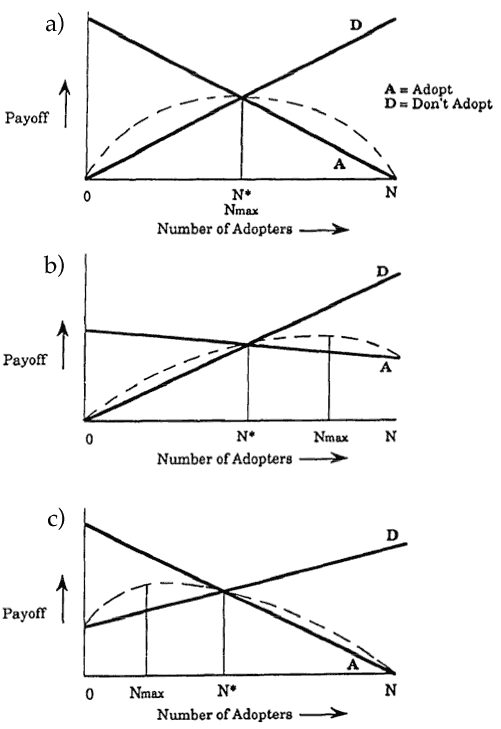
\includegraphics[width=1\linewidth]{gfx/markusCongestedTextProcessor}}
		\caption[>>Payoff<< durch Nutzung zweier Textverarbeitungsmaschinen \newline \citep{Markus:1990}]{Die Grafiken illustrieren drei Szenarios der Entwicklung des tatsächlichen Nutzen (>>Payoff<<) für die Abteilung durch Einführung eines zweiten Computers mit einem Textverarbeitungsprogramm.}\label{fig:markusText}
\end{figure}
	
	Der Abteilungsleiter entscheidet daher, einen zweiten Computer anzuschaffen und teilt dies der Belegschaft mit. In dieser Situation ist es wahrscheinlich, dass das Verhalten der Mitarbeiter den maximalen Nutzen der zweiten Maschine verhindert. Jeder hat zwei Optionen offen und kann entweder auf den neuen Computer umsteigen (\emph{A} für >>Adopt<<) oder beim alten bleiben (\emph{D} für >>Don't Adopt<<). \hyperref[fig:markusText]{Abbildung \ref*{fig:markusText}a} zeigt eine theoretische Verteilung des tatsächlichen Nutzen der Einführung des zweiten Computers. Auf der horizontalen Achse ist die Anzahl der Mitarbeiter dargestellt, die auf das neue Gerät wechseln. \emph{N} bezeichnet die Gesamtanzahl aller Mitarbeiter. Die Linien \emph{A} und \emph{D} sind linear invers zueinander und stellen die Auslastung der beiden Geräte dar. Diese ergibt sich aus der Anzahl der jeweiligen Nutzer. Die vertikale Achse zeigt den Nutzen für die gesamte Abteilung. Theoretisch erreicht man einen maximalen Nutzen für die Abteilung, wenn beide Geräte gleich ausgelastet sind, in der Praxis jedoch ist dies oft nicht der Fall.
	
	\medskip Es gibt viele Faktoren, die den Verlauf von \emph{A} und \emph{D} beeinflussen können, beispielsweise unterschiedliche Rechenleistungen und Performance der beiden Computer oder der Aufwand, der mit dem Erlernen eines neuen User Interface am neuen Rechner verbunden ist. \hyperref[fig:markusText]{Abbildung \ref*{fig:markusText}b} und \hyperref[fig:markusText]{Abbildung \ref*{fig:markusText}c} zeigen zwei weitere mögliche Szenarios, bei denen der maximale Nutzen dann erreicht wird, wenn der größere Teil der Belegschaft entweder beim alten Gerät bleibt oder zum neuen wechselt.
	
	Dieses Beispiel zeigt, dass es notwendig ist, spezielle Situationen genau zu analysieren und entsprechend darauf zu reagieren. So läge es hier am Abteilungsleiter, die optimale Auslastung der beiden Geräte zu finden und zu forcieren. Die gegenseitige Abhängigkeit, die in solch einem Szenario entsteht, ist der Grund für diese unterschiedlichen Ergebnisse \citep{Markus:1990}.
	
	\medskip Als zweites Beispiel behandeln Markus und Connolly ein System zur automatischen Planung von Meetings, genauso wie Jonathan Grudin in seiner Studie \citep{Grudin:1988p126}. Dieses System wird für eine Gruppe von Personen in einem Unternehmen eingeführt, die untereinander alle ungefähr gleich vielen Meetings beiwohnen. Damit sei gesichert, dass theoretisch jeder gleich viel vom System profitieren kann. 
	
	In diesem Szenario sind >>Adopter<< jene Personen, die regelmäßig ihre Termine in das System eintragen und pflegen. Sobald Termine eingetragen werden, sind sie für alle zugänglich. Daher haben >>Non-Adopter<< einen Vorteil: sie haben keinen zusätzlichen Aufwand, da sie nichts eintragen, trotzdem verfügen sie über alle Informationen im System. Diese Situation kann auch als >>multi-person prisoner's dilemma<< bezeichnet werden \citep{Schelling:1987}.

\begin{figure}
	{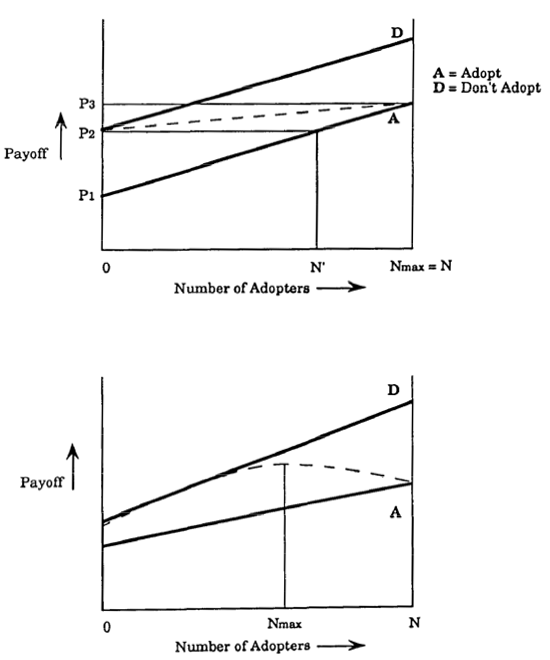
\includegraphics[width=1\linewidth]{gfx/markusMeetingPlanner}}
\caption[>>Payoff<< durch Nutzung eines automatischen Meeting Planers \newline \citep{Markus:1990}]{Die Grafiken illustrieren zwei Szenarios der Entwicklung des tatsächlichen Nutzen (>>Payoff<<) für die Abteilung durch Einführung eines automatischen Meeting Planers.}\label{fig:markusMeeting}
\end{figure}

In \hyperref[fig:markusMeeting]{Abbildung \ref*{fig:markusMeeting}a} wird der Nutzen von >>Adoptern<< und >>Non-Adoptern<< als zwei parallele Linien dargestellt. Die Differenz dieser beiden Werte bezeichnet den zusätzlichen Aufwand, den nur >>Adopter<< haben. Deswegen ist ihr Nutzen geringer. Man erkennt sofort, dass es irrelevant ist, wie viele Personen das System nutzen und wie viele nicht, denn diejenigen, die es nicht nutzen, werden immer einen Vorteil haben. Dies bedeutet aber auch, dass es für jeden das Beste wäre, das System nicht zu nutzen, weshalb es zu Schwierigkeiten bei der Einführung eines solchen Systems kommen könnte. In so einem Fall läge es wiederum am Abteilungsleiter, entsprechende Maßnahmen zu ergreifen, damit sich dieses ungleiche Verhältnis verbessert. 

\hyperref[fig:markusMeeting]{Abbildung \ref*{fig:markusMeeting}b} zeigt eine Situation, in der sich ausreichen Mitarbeiter zusammenschließen und gemeinsam in einer Koalition das System nutzen. Sie schaffen dadurch den selben kollektiven Nutzen für >>Adopter<<, wie wenn keiner das System verwenden würde. Dies setzt natürlich voraus, dass die Koalition über genügend Mitglieder verfügt, da die Rechnung sonst nicht aufgeht.

\medskip Im letzten Beispiel erläutern Markus und Connolly die Relevanz der kritischen Masse. Sie untersuchen dazu ein neu eingeführtes Kommunikationssystem, das es den Mitarbeitern erlaubt, intern mittels E-Mail zu kommunizieren. Vor Einführung dieses neuen Systems standen den Angestellten das Telefon, face-to-face Meetings und interne Post als Kommunikationsmittel zur Verfügung. 

Es ist offensichtlich, dass der Nutzen dieses neuen Mediums für die ersten >>Adopter<< relativ gering ist. Genauso wie das Telefon macht das E-Mail System wenig Sinn, wenn es nicht von jedem genutzt wird. Gibt es aber genügend Personen die es nutzen, steigt der Nutzen für alle stark an, unter Umständen sogar so weit, dass er den Nutzen anderer Kommunikationskanäle übersteigt. 

\medskip \hyperref[fig:markusMass]{Abbildung \ref*{fig:markusMass}a} zeigt den Punkt der kritischen Masse dort, wo die >>Payoff<< Linien von >>Adoptern<< und >>Non-Adoptern<< sich schneiden. Der tatsächliche Nutzen für das Kollektiv wird durch die gestrichelte Linie dargestellt. Für das einzelne Individuum ist es vor Erreichen der kritischen Masse vorteilhafter, nicht auf das neue System umzusteigen, doch nach Erreichen der kritischen Masse ist das Umsteigen vorteilhafter. Der steigende Nutzen vor der kritischen Masse für >>Non-Adopter<< ergibt sich aus der Annahme, dass durch mehr >>Adopter<< weniger Personen die alten Kommunikationsmittel nutzen und diese dadurch entlastet werden. >>Non-Adopter<< finden also leichter freie Räume für Meetings und kommen auf telefonischem Wege leichter zu anderen Mitarbeitern durch, da deren Linien seltener besetzt sind. In dieser Situation erreicht der Nutzen für das kollektiv seinen Höchststand, wenn alle Mitarbeiter das neu System verwenden. 

\medskip \hyperref[fig:markusMass]{Abbildung \ref*{fig:markusMass}b} stellt einen sinkenden Nutzen für >>Non-Adopter<< dar, während die Anzahl der >>Adopter<< steigt. Diese Situation könnte beispielsweise eintreten, wenn Personen wichtige Informationen nicht erhalten, nur weil sie das neue E-Mail System nicht nutzen. Höchst interessant ist in dieser Illustration die Tatsache, dass, wenn niemand das neue System verwendet, ein gleich hoher Nutzen für das Kollektiv entsteht, wie wenn alle es verwenden.

\begin{figure}
	{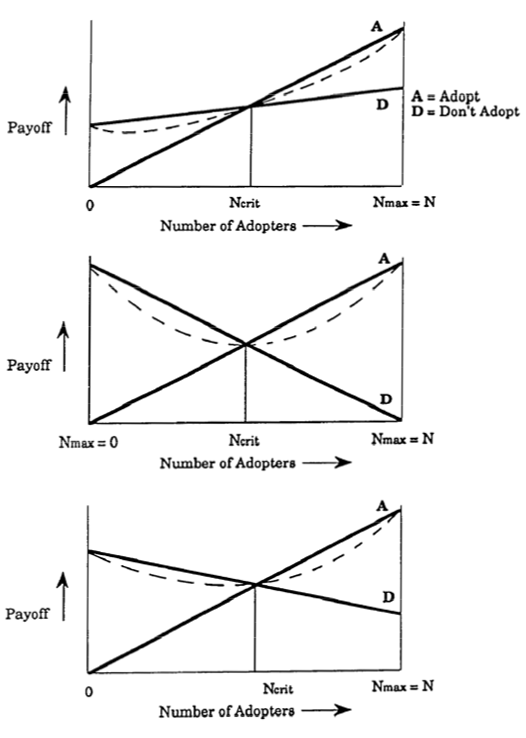
\includegraphics[width=1\linewidth]{gfx/markusCriticalMass}}
\caption[Die kritische Masse \newline \citep{Markus:1990}]{Die Grafiken illustrieren drei Szenarios der kritischen Masse unter verschiedenen Umständen.}\label{fig:markusMass}
\end{figure}

\medskip \hyperref[fig:markusMass]{Abbildung \ref*{fig:markusMass}c} geht von einem noch pessimistischeren Szenario aus und zeigt den maximalen Nutzen wenn jeder Mitarbeiter auf das neue System umsteigt. Wichtig ist hier jedoch die Tatsache, dass die Belegschaft besser dran ist, wenn keiner umsteigt, als wenn nur einige, sprich weniger Personen als für die kritische Masse notwendig, umsteigen. Das bedeutet, solange die Rate der Umsteiger sich nicht 100\% nähert, ist es vorteilhafter, wenn keiner der Mitarbeiter umsteigt.

\medskip Aus diesen designierten Szenarios wird ersichtlich, dass die gegenseitigen Abhängigkeiten, denen Groupware unterliegt, eng verknüpft sind mit Nutzen und Schaden, die das jeweilige System anrichten kann. Diese Eigenheiten müssen beim Design von Groupware beachtet werden, damit der Erfolg selbiger nicht gefährdet ist. \citep{Markus:1990}

\section*{Zusammenfassung}
In der Wissenschaft gibt es verschiedene Definitionen und Auslegungen des Begriffes >>Computer Supported Cooperative Work<<. Die Wurzel dieser Uneinigkeit findet sich schon tiefer, bei der genauen Definition und Unterscheidung von >>Collaborative Work<<, >>Collective Work<< und >>Cooperative Work<<. Viele Wissenschaftler verwenden die Begriffe synonym, andere hingegen bestehen auf einer klaren Trennung der Termini. Für die Zwecke dieser Arbeit reicht jedoch eine synonyme Verwendung aus, denn letztendlich bezeichnet der Begriff \ac{CSCW} ein multidisziplinäres Forschungsgebiet, das kooperative Zusammenarbeit innerhalb Gruppen untersucht und Technologien zur Förderung und Unterstützung selbiger entwickelt. Unter >>Groupware<< versteht man alle Systeme, egal ob Hard- oder Software, welche die in \ac{CSCW} gewonnenen Erkenntnisse in die Praxis, zum Zwecke der Verbesserung von Teamwork, umsetzen. Design und Entwicklung solcher Systeme ist eine schwierige Aufgabe und wird von vielen verschiedenen Faktoren beeinflusst, die über Erfolg oder Misserfolg entscheiden. Es gibt Frameworks und Patterns, die versuchen formale Richtlinien zu geben, jedoch bildet jedes System und vor allem das Umfeld, in dem es eingesetzt wird, einen einzigartigen Kontext, der genau analysiert und berücksichtigt werden muss.


\cleardoublepage\part{Praxis}
%*************************************************************
\chapter{Scribbler}\label{ch:scribbler} \index{Scribbler}
%*************************************************************

Die vergangenen Kapitel zeigen viele Beispiele, wie und mit welchen Hilfsmitteln Gruppenmeetings abgehalten werden können. Seien es traditionelle Medien wie Papier und Flip-Charts, oder elektronische Medien wie computerunterstützte Whiteboardsysteme - sie alle finden Einsatz in Designsessions und bieten verschiedenste Vor- und Nachteile.

\medskip Im folgenden wird \scribbler vorgestellt, ein elektronisches Interface, das die kollaborative Arbeit an virtuellen Artefakten unterstützt. Ähnlich wie die Autoren der bereits im ersten Kapitel beschriebenen Systeme, wurde mit \scribbler versucht, ein System zu kreieren, das die beiden Design-Arbeitswelten - geprägt durch traditionelle und elektronische Medien - mit einander verbindet und ihre Vorteile herausarbeitet. Im Gegensatz zu den bisherigen Ansätzen ist \scribbler ein elektronisches Skizziersystem, das ein barrierefreies Arbeiten ermöglicht.

\medskip Um dies zu zeigen, wird zuerst kurz die Ausgangssituation geschildert und danach die Anforderungen an ein kollaboratives Skizziersystem, die sich aus der Literaturrecherche ergeben haben, präsentiert. Danach wird die Vorgehensweise zur Erstellung des Prototyps erklärt, welche selbst einige Designmethoden aus \autoref{ch:designTheorie} beinhaltet. Anschließend folgt eine Präsentation der simplen Oberfläche von \scribbler und dessen Funktionsumfang mitsamt technischer Hintergründe. Schlussendlich werden die Anforderungen und Merkmale gegenübergestellt und die aus User-Tests gewonnenen Erkenntnisse beschrieben.

\section{Ausgangssituation \& Rahmenbedingungen} \label{sec:ausgangssituation} \index{Scribbler!Ausgangssituation}
Die Technisierung vieler Berufe führte dazu, dass gewisse Arbeitsgegenstände ein elektronisches Abbild bekamen. Im Gegensatz zu früher, fertigen Grafikdesigner heutzutage Präsentationszeichnungen oft an einem digitalen Medium an. Neuere Berufssparten wie Interfacedesign setzen die tagtägliche Arbeit mit digitalen Artefakten voraus. Wie schon in den vorigen Kapiteln erwähnt, ist (im Besonderen) Design eine kollaborative Tätigkeit, wofür sich Gruppen in Meetings treffen, um gemeinsam neue Lösungen zu erarbeiten. Ein bewährtes und wichtiges Instrument dazu sind Stifte zur Erstellung von Skizzen, um Gedanken auszudrücken.

Ein wesentlicher Bestandteil moderner Meetingräume ist ein zentraler Bildschirm oder Projektor, der als Präsentationsmedium eingesetzt wird. Zudem ist meistens eine Zeichenfläche vorhanden, wie z.B. Whiteboards oder Flip-Charts, um kollaborativ erarbeitete Ideen festzuhalten und neue Ideen zu explorieren.

\medskip Das Institut für Gestaltungs- und Wirkungsforschung an der TU Wien verfügt über so einen Meetingraum. Darin befinden sich mehrere Tische, die in der Mitte des Raumes zusammengestellt wurden und um die sich Sitzmöglichkeiten befinden. Neben einem Flip-Chart befindet sich ein {54\dq} großer Bildschirm in der Mitte einer Wand, auf den alle Meetingteilnehmer von ihren Sitzplätzen aus blicken können. Mit dem Screen ist ein Computer (Apple Mac Mini) verbunden, auf den Daten über ein drahtlos Netzwerk gespielt werden können. Eine zusätzliche drahtlose Tastatur und Maus ermöglichen eine bequeme Steuerung. Zusätzliche Peripherie kann an der Rückseite des Computers angeschlossen werden.

\medskip Das Kerngebiet des Instituts ist \ac{HCI}. Hier wird der Meetingraum oft dazu verwendet, Designs für interaktive Systeme, Applikationen oder Webinhalte zu erarbeiten. Erwartungsgemäß sind nur bereits umgesetzte Inhalte digital vorhanden. Diese Problematik macht den Einsatz der wichtigsten Designmethode - Skizzieren - auf dem Artefakt fast unmöglich. Das Ziel der vorliegenden Arbeit war es nun ein Tool zu entwickeln, das es ermöglicht, auf jegliche präsentierte Inhalte ob Webseiten, Programmoberflächen oder Bilder, >>kritzeln<< zu können. \scribbler soll so die Barriere zwischen der realen Welt und der digitalen Welt aufbrechen.

\section{Anforderungen an kollaborative Skizziersysteme} \label{sec:anforderungen} \index{Skizziersysteme!Anforderungen}
In den vorhergehenden Kapiteln wurde ein Überblick über das Verbesserungspotential vieler existierender Systeme gegeben. Wichtige literarische Größen auf diesem Gebiet, wie beispielsweise Lee, Olsen, Tang, Larsson, Johnson oder Prante, wiesen auf wesentliche Erkenntnisse hin, die ein solches System formen. Diese Erkenntnisse können vier großen Einflussfaktoren zugeordnet werden: \emph{Hardware}, \emph{Software}, \emph{Kollaboration} und \emph{Skizzieren} und bieten eine Art Checkliste für kollaborative Systeme. \autoref{fig:scribblerKollaborativesSkizziersystem} zeigt eine Aufstellung dieser Erkenntnisse, in Verbindung zu ihren Einflussfaktoren. 

\begin{figure}
	        {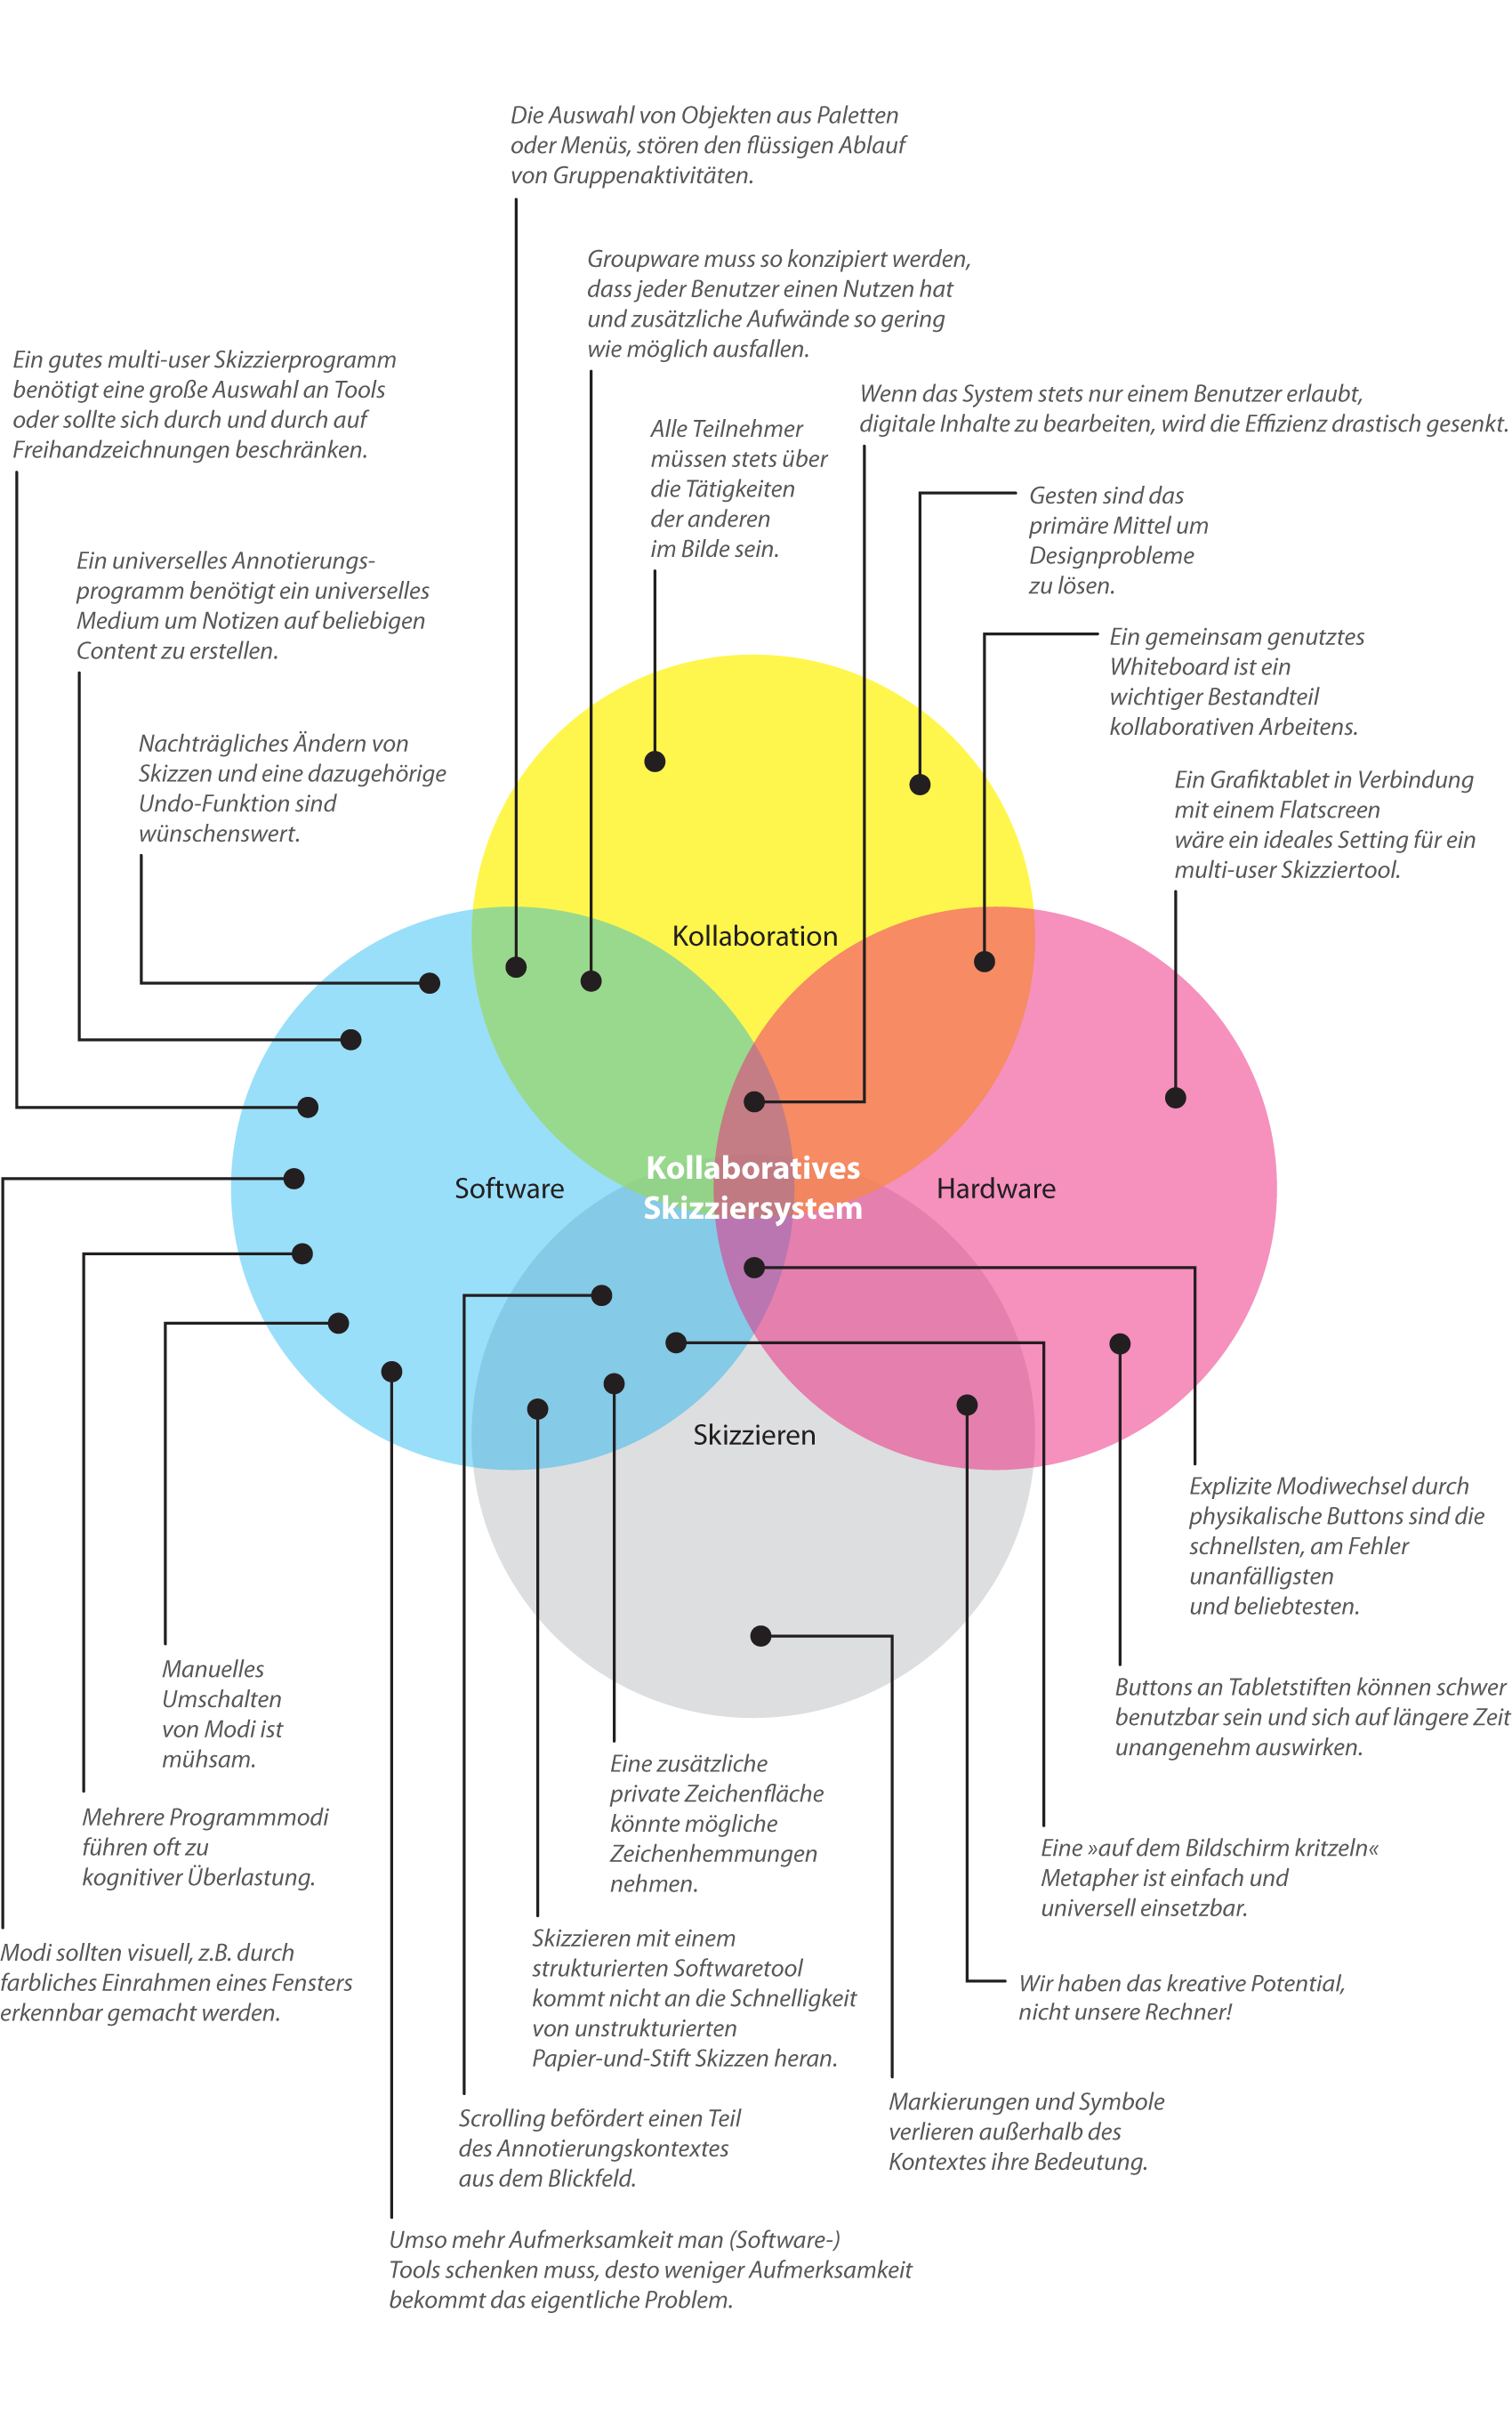
\includegraphics[bb=0cm 0cm 14.39cm 23.01cm]{gfx/scribblerKollaborativesSkizziersystem}}
		\caption[Anforderungen eines kollaborativen Skizzersystems]{Anforderungen eines kollaborativen Skizzersystems, bestehend aus den vier Einflussfaktoren: Hardware, Software, Kollaboration \& Skizzieren.}\label{fig:scribblerKollaborativesSkizziersystem}
\end{figure}

\subsubsection*{Hardware} Ein ideales Setting für ein kollaboratives Skizziertool wäre laut Lee ein Grafiktablet in Verbindung mit einem Flatscreen. Dies wäre die bestmögliche Annäherung an eine Technologie, die Stift und Papier ersetzen könnte. Sie würde ebenso zur Umsetzung eines Whiteboard Systems beitragen, was einen wichtigen Bestandteil kollaborativen Arbeitens ausmacht. Buttons an Tabletstiften können schwer benutzbar sein und sich auf längere Zeit unangenehm auswirken, deswegen sollte davon abgeraten werden diese mit Funktionen zu belegen. 

\subsubsection*{Software} Ein gutes multi-user Skizzierprogramm benötigt eine große Auswahl an Tools oder sollte sich ausschließlich auf Freihandzeichnungen beschränken. Welcher Ansatz besser funktioniert, müsse laut Lee ausprobiert werden. Je mehr Aufmerksamkeit ein Softwaretool erfordert, desto weniger Aufmerksamkeit kann jedoch dem eigentlichen Problem zukommen. Folglich sollte solch ein System so einfach wie möglich aufgebaut sein.

Die Verwendung mehrerer Programmmodi führt oftmals zu kognitiver Überlastung. Aus diesem Grund sollte der aktuelle Modus visuell, z.B. durch farbliches Einrahmen eines Fensters, erkennbar gemacht werden. Zudem ist das manuelle Umschalten von Modi mühsam. Explizite Modiwechsel durch physikalische Buttons sind dennoch die schnellsten, am Fehler unanfälligsten und beliebtesten. 

Will man ein universelles Annotierungstool schaffen, das über alle verwendeten Programme eines Benutzers funktioniert, benötigt man auch ein universelles Medium, um Notizen auf beliebigem Content zu erstellen. Außerdem wären das nachträgliche Ändern von Skizzen und eine dazugehörige Undo-Funktion wünschenswert.

\subsubsection*{Kollaboration} Gemeinsam genutzte Systeme müssen so konzipiert werden, dass jeder Teilnehmer einen Nutzen hat. Wenn das System nur einem Benutzer erlaubt digitale Inhalte zu bearbeiten, wird die Effizienz drastisch gesenkt. Zusätzliche Aufwände sollten so gering wie möglich ausfallen. Die Auswahl von Objekten aus Paletten oder Menüs, stören beispielsweise den flüssigen Ablauf von Gruppenaktivitäten. Die Teilnehmer der Kollaboration sollten ebenso stets über die Tätigkeiten der anderen im Bilde sein. Dabei spielen Gesten eine wichtige Rolle.

\subsubsection*{Skizzieren} Das Zeichnen mit einem strukturierten Softwaretool ersetzt nicht das Zeichnen von unstrukturierten Papier-und-Stift Skizzen. Eine >>auf dem Bildschirm kritzeln<< Metapher ist somit einfach und universell einsetzbar. Skizzen verlieren außerhalb des Kontextes ihre Bedeutung. Daher muss darauf geachtet werden, dass der Kontext stets bewahrt wird. Scrolling befördert z.B. einen Teil des Annotierungskontextes aus dem Blickfeld und benötigt somit zusätzliche Aufmerksamkeit bei der Umsetzung. Außerdem könnte eine zusätzliche, private Zeichenfläche mögliche Zeichenhemmungen von Teilnehmern nehmen. Schlussendlich haben die Benutzer das kreative Potential - ein Skizziersystem muss sich entsprechend adaptieren können.

\section{Vorgehensweise} \index{Scribbler!Vorgehensweise}
Aufgrund des Bedarfs nach einem elektronischen Skizziersystem wurde zuerst eine Suche nach vergleichbaren Systemen veranlasst. Eine Brainstorming-Sitzung diente dazu, verschiedene Begriffe zu sammeln und zu explorieren. Viele wissenschaftliche Datenbanken stellen eine Fülle an Literatur bereit, die wiederum Hinweise zu bestehenden kollaborativen Skizziertools liefert. Nach der Lektüre und Analyse der gesammelten Werke konnte ein vorläufiges Anforderungsprofil an solche Systeme erstellt werden.

Eine wichtige Designfrage stellte sich schon zu diesem Zeitpunkt: Welche Eingabetechnologie sollte für \scribbler eingesetzt werden? \autoref{fig:scribblerVorgehensweise} zeigt Aufzeichnungen zu der wohl wichtigsten hardwarespezifischen Frage. Nachträglich digitalisierte Skizzen, würden das System unabhängig von notwendigen Gerätschaften machen. Diese Voraussetzung käme der Flexibilität des Systems zu Gute. Jedoch ist es technisch aufwändig und fehleranfällig, gezeichnete Objekte nachträglich zu erkennen. Es müsste Mustererkennung zum Einsatz kommen, und das Ergebnis könnte unter Umständen nicht zufriedenstellend ausfallen. Würden Zeichnungen direkt auf digitalem Wege angefertigt, z.B. via Tablets, wäre die Flexibilität des Systems zwar eingeschränkt, das Ergebnis jedoch besser.

Im Hinblick auf \scribbler wurde zusammen mit dem Institut entschieden, auf die zweite Variante zu setzen, da Tablets bereits vorhanden waren und für einen ersten Prototypen ausreichen sollten.

\begin{figure}
	        {\includegraphics[width=1\linewidth]{gfx/scribblerVorgehensweise}}
		\caption[Aufzeichnung zur frühesten Designfrage]{Aufzeichnung zur frühesten Designfrage. Sollten Skizzen nachträglich digitalisiert werden oder sollte gleich auf digitales Zeichnen gesetzt werden?}\label{fig:scribblerVorgehensweise}
\end{figure}

Nachdem das grobe Konzept geklärt war, folgte der nächste Schritt, das Verstehen des eigentlichen Skizzierens. Es wurden dazu verschiedene Szenarios exploriert, um einen Einblick in die Praxis der Thematik zu erlangen. Anschließend wurden mehrere Mockups erstellt und das Skizzierverhalten von verschiedenen Probanden analysiert. Das Konzept konnte dadurch nach und nach verfeinert werden, doch aussagekräftigere Tests waren notwendig. Aus diesem Grund wurde bald mit der Anfertigung von Prototypen mit größerem Funktionsumfang begonnen. Die Mockups konnten auch nur Ein-Benutzer-Szenarios abdecken, weshalb schon bald mit der Implementierung begonnen wurde.

\bigskip \emph{Anmerkung: \graffito{\(\clubsuit\)} Zu diesem Zeitpunkt kam erstmals der Begriff >>Scribbler<< auf, der fortan als Codename für das Projekt benutzt wurde.}
\bigskip

Während der Implementierungsphase konnten Funktionalität und Verhalten des Systems durch interne Tests kontinuierlich verbessert werden. Mit Hilfe von potentiellen Nutzern wurde die finale Beta-Version von \scribbler einem Review unterzogen.

\medskip In den folgenden Punkten werden die angesprochenen und verwendeten Designmethoden (vgl. \autoref{sec:designmethoden}) beschrieben und mit Hilfe verschiedener Bilder veranschaulicht. Die Beschreibung des Designprozesses soll so angereichert und durch konkrete, praktische Beispiele verständlicher aufbereitet werden.

\subsection{Recherche}
Recherche ist nicht direkt den Designmethoden zuzuordnen, stellt aber trotzdem einen wichtigen Teil in der Entwicklung eines Produkts dar. Recherche ermöglicht Einsicht in den betehenden Markt und die aktuelle Forschung. Des weiteren wird ein Einblick in deren Funktionsweisen erlangt.

\medskip Durch die Literaturrecherche wurden einige vergleichbare Systeme gefunden, die jedoch die große Einschränkung hatten, dass Content und Input nicht miteinander verknüpft wurden. Es gibt zwar Annäherungen, jedoch bringen diese den Inhalt nur in eine statische Scheinbeziehung mit den Eingaben. Dies verdeutlichte die Notwendigkeit eines Skizziersystems wie \scribbler, das über die Grenzen des Instituts hinausgehen könnte.

Zusätzlich wies die Literatur bereits auf Probleme hin, die durch die notwendige Selektion eines Werkzeuges entstehen konnten (vgl. \pointref{sec:ModusProblem}).

\medskip Das Erlangen neuer Sichtweisen des Systems durch die ausgiebige Recherche resultierte schließlich im vorläufigen Anforderungsprofil.

\subsection{Skizzieren}
Alleiniges bzw. gemeinsames Skizzieren waren die wichtigsten Instrumente in der Anfangsphase von \scribbler. Skizzen ermöglichten die Veranschaulichung bzw. Generierung neuer Ideen und dienten somit auch als Diskussionsbasis. 

Aus der Literaturrecherche geht hervor, dass meistens ein Sitzungsteilnehmer als Schreiber fungiert und die wichtigsten, besprochenen Fakten in Stichwörtern und kurzen Sätzen zusammenfasst (vgl. \autoref{fig:scribblerVorgehensweise}). Skizzen wurden manchmal angefertigt um bestimmte Vorgehensweisen aus der Literatur zu illustrieren. Dies führte meist zu kollaborativen Arbeitsvorgängen, bei denen zusammen an einer Skizze gearbeitet wurde. 

\medskip Wie bereits erwähnt, wurden später Skizzen zu wichtigen Szenarios erstellt. Eine farbliche Kennzeichnung war dabei oft sehr hilfreich. Zudem konnten Zugehörigkeiten oder zeitliche Abläufe durch Hinzufügen von Nummerierungen leicht angedeutet werden (siehe \autoref{fig:scribblerSzenarien}).

\medskip Abschließend zeigt \autoref{fig:scribblerDetailSkizze} ein Beispiel einer detaillierten Skizze, die dazu verwendet wurde, technische Abläufe zu verstehen. Sie entstand im Laufe der Entwicklung, in der ständig neue Ideen aufkamen, die durch Skizzen innerhalb des Teams erforscht wurden.

\begin{figure}
	\begin{center}
	        {\includegraphics[width=0.8\linewidth]{gfx/scribblerSzenarien}}
		\caption[Skizzierte Szenarien in Scribbler]{Skizzierte Szenarien in Scribbler. Zugehörigkeiten wurden durch eine Nummerierung gekennzeichnet.}\label{fig:scribblerSzenarien}
	\end{center}
\end{figure}

\begin{figure}
	        {\includegraphics[width=1\linewidth]{gfx/scribblerDetailSkizze}}
		\caption[Detailskizze eines technischen Ablaufs]{Detaillierte Skizze eines technischen Ablaufs, um diesen besser zu verstehen.}\label{fig:scribblerDetailSkizze}
\end{figure}

\subsection{Prototyping}
Das Erarbeiten von Prototypen war keine leichte Aufgabe, da das Setting an sich, durch die verschiedenen Einflussfaktoren, kompliziert erschien. Dennoch konnten anfangs simple Prototypen, sogenannte Mockups angefertigt werden, um vorerst detailliertere Szenarios zu erstellen und später das Skizzierverhalten einiger Probanden zu beobachten. Mockups sind low-fidelity Prototypen, beispielsweise Papierprototypen. Dieser >>Wegwerfcharakter<< impliziert eine einfache Erstellung und rudimentäre Funktionalität, die für frühe Tests ausreicht.

\medskip \autoref{fig:scribblerMockups} zeigt ein Mockup, das im Wesentlichen nur aus einem Screenshot eines \acs{WIMP}-Systems bestand (in diesem Fall Mac OS X mit zwei offenen Programmfenstern) und in Verbindung mit einem Tablet PC benutzt wurde. Die konzipierten Szenarios, wurden durch den höheren Detailgrad konkreter, wodurch mehrere Funktionen im Voraus geplant werden konnten. Später wurden diese verwendet, um erste Tests durchzuführen. Der Prototyp beschränkte die Interaktionen der Benutzer auf das Skizzieren. So konnte beispielsweise festgestellt werden, welche Plätze zum Zeichnen gesucht werden, wie bestimmte Elemente markiert werden oder Zusammenhänge von Inhalten hergestellt werden.

\begin{figure}
	        {\includegraphics[width=1\linewidth]{gfx/scribblerMockups}}
		\caption[Mockups in Scribbler]{Simple Mockups, die durch Screenshots auf einem Tablet PC erstellt wurden.}\label{fig:scribblerMockups}
\end{figure}

\medskip Darauf folgende Prototypen als programmierte Versionen von \scribbler wurden ebenfalls getestet.

\subsection{(User-) Testing}
Die erstellten Prototypen vor der Implementierung des Programms, ermöglichten die Testung eines kleinen Funktionsteils mit Usern. Wichtige Systemverhaltensweisen bzw. Interaktionen konnten aber nur durch zusätzliche Testdurchgänge während der Umsetzung, auf Verständlichkeit und Anklang geprüft werden.

\medskip Einen Vorteil stellte die geringe Vorbereitungszeit dar. Es mussten keine bestimmten Anweisungen oder Aufgaben gestellt werden. Zum einen sollte die reale Welt in Bezug auf das Skizzieren mit Papier und Stift nachgebildet werden. Zum anderen sollten keine aufwändigen Aufgaben notwendig sein, sodass Probanden einfach >>loskritzeln<< konnten.

\medskip Es bestand außerdem die Möglichkeit, \scribbler innerhalb einer Gruppe von fünf Personen zu testen, die an einem bestimmten Design arbeiteten und dazu den in \autoref{sec:ausgangssituation} beschriebenen Meetingraum vom Institut nutzten (siehe \autoref{fig:scribblerUserTest}).

\begin{figure}
	        {\includegraphics[width=1\linewidth]{gfx/scribblerUserTest}}
		\caption[Scribblertesting in einer Designsession]{Scribblertesting in einer Designsession. Fünf Personen überarbeiten mittels Scribbler ein Designvorschlag.}\label{fig:scribblerUserTest}
\end{figure}

\medskip Nach Fertigstellung der Betaversion konnte \scribbler zusätzlich am Beginners-Day\footnote{Der Beginners-Day ist eine Infoveranstaltung für alle Studienanfängerinnen und Studienanfänger in den Informatik-, Wirtschaftsinformatik- und Lehramtsstudien. \citep{TU:2010}} der TU Wien vorgeführt und mit vielen erstsemestrigen Studenten getestet werden. Abschließend konnten auch ausführliche Tests mit Designern durchgeführt werden, die in \autoref{sec:userReview} ausführlich beschrieben sind.

\section{Scribbler at a Glance} \index{Scribbler!at a Glance}
Durch die verschiedenen Designmethoden veränderte sich die Funktionalität von \scribbler öfters. Aus diesem Grund wird das Konzept erst in diesem Kapitel angeführt.

\medskip \scribbler ermöglicht neben der herkömmlichen Arbeit an einem Desktop (\acs{WIMP}) System, mittels Stiften auf jedes beliebige Programmfenster zu zeichnen. Das System läuft im Hintergrund und aktiviert sich bei Bedarf. Es unterscheidet dabei generell zwei Hauptmodi: den Zeichen- und den Mausmodus. In letzterem kann die Maus wie gewohnt zur Navigation zwischen Programmfenster eingesetzt werden. Die Verwendung eines Tabletstifts hingegen wechselt in den Zeichenmodus. Die Benutzer können so auf das momentan aktive Fenster einer Drittapplikation >>kritzeln<<. Da besonders geübte Tabletbenutzer die Stifte auch als Ersatz für die Maus verwenden, ermöglicht \scribbler auch das explizite Wechseln der beiden Modi durch Drücken einer Tablettaste.

\medskip Da beim Skizzieren natürlich auch Fehler auftreten können, bietet \scribbler eine >>Undo<< bzw. >>Redo<< Funktion. Versehentliche Aktionen können so rückgängig gemacht oder wiederhergestellt werden. Zudem können einzelne Striche gelöscht bzw. >>ausradiert<< oder der gesamte Zeichenbereich geleert werden.

\medskip Diese Grundfunktionalität soll vor allem Designer die Möglichkeit bieten, bestehende Arbeiten und Designs zu besprechen, Anmerkungen in direkter Verbindung zu digitalen Artefakten zu verfassen und kontextbezogene Erweiterungen zu zeichnen. Weil natürlich nicht immer schon vorhandene Designs vorliegen, bietet \scribbler aber auch eine Whiteboard Funktion. Hierbei wird eine weiße Fläche über den gesamten Bildschirm eingeblendet, auf dem Benutzer Raum zum freien Skizzieren bekommen.

\medskip Um erarbeitete Skizzen zu speichern, besitzt \scribbler eine Screenshot Funktion. Nur durch Speichern eines Bildes, kann aus unserer Sicht der Kontext zu den Zeichnungen bewahrt werden. Eine Unterbrechung, jedoch nicht Beendigung von \scribbler, erfolgt durch eine integrierte Standby Funktion.

\medskip Die folgenden Punkte sollen nun nähere Informationen zur Hardware, dem grafischen User Interface und dem logischen Programmaufbau geben. 

\subsection{Hardware} \label{ssec:hardware} \index{Scribbler!Hardware}
\scribbler benötigt ein relativ komplexes Hardware-Setting. Für die Ausgabe wird ein großes Display oder ein Beamer benutzt, während es für die Eingabe erforderlich ist, dass jeder Benutzer über ein Tablet mit Stift verfügt. Diese Tablets und das Ausgabegerät werden mit einem Rechner verbunden, auf dem das Apple Betriebssystem OS X 10.6 >>Snow Leopard<< läuft. Ältere Versionen von OS X werden von \scribbler nicht unterstützt. Für ein optimales Nutzungserlebnis sollte der Computer über eine gute Rechenleistung verfügen. Bei der Umsetzung des Prototypen fiel die Entscheidung auf die Nutzung von Tablets aus der Modellreihe Intuos3 von Wacom. Diese Geräte verfügen über jeweils vier Buttons an beiden Seiten neben der Zeichenoberfläche, die mit verschiedenen Funktionen belegt werden können. Über diese Tasten können die folgenden Aktionen durchgeführt werden:

\begin{itemize}
	\item \emph{Wechsel des Interaktionsmodus für den Tabletstift}\\
	Ermöglicht das Umschalten von Zeichen- in den Mausmodus und umgekehrt. (Dies betrifft nur den Tabletstift, die Maus selbst ist immer im Mausmodus und kann nicht zum Zeichnen verwendet werden)
	\item \emph{Whiteboard}\\
	Blendet eine weiße Fläche über den gesamten Screen ein oder aus. Auf dieser kann ebenfalls gezeichnet werden.
	\item \emph{Zurücksetzen}\\
	Löscht alle Zeichnungen des momentan aktiven Fensters.
	\item \emph{Sichern}\\
	Erstellt einen Schnappschuss des Bildschirm samt den Zeichnungen des aktiven Fensters und legt diesen in einer Datei am Schreibtisch ab.
\end{itemize}

\begin{figure}
	\begin{center}
        {\includegraphics[width=0.8\linewidth]{gfx/scribblerTabletTasten}}
		\caption[Tablet Tastenbelegung]{Die Anordnung der \scribbler Funktionen auf den Tasten des Tablets. Der Fotoapparat links oben erstellt ein Bildschirmfoto, das Verbotszeichen auf der rechten, oberen Taste löscht alle Zeichnungen des aktiven Fensters, die Maus auf der genoppten, mittleren Taste wechselt den Interaktionsmodus und das Whiteboard auf der unteren Taste blendet selbiges ein oder aus.}\label{fig:scribblerTabletTasten}
	\end{center}
\end{figure}

\autoref{fig:scribblerTabletTasten} zeigt die Anordnung der Buttons auf den Tablets. Die mittlere Taste ist mit einer Noppe versehen und bietet dadurch ein haptisches Feedback. Dadurch kann der Button ertastet werden ohne dass ein Hinsehen von Nöten ist. Sinnvollerweise sollte diese Taste mit der wichtigsten Funktion belegt werden. In \scribbler ist dies der Wechsel des Interaktionsmodus, denn dieser ermöglicht, den vollen Interaktionsumfang mit nur einem Eingabegerät (dem Stift) zu nutzen. Die anderen beiden wichtigen Funktionen, sprich das Bildschirmfoto und das Whiteboard, liegen auf den zwei großen Tasten links oben und unten. Das Zurücksetzen aller Zeichnungen wird relativ selten gebraucht und liegt daher auf der kleinen Taste rechts oben. Damit Benutzer diese Anordnung nicht auswendig lernen müssen, wurden bei den Tests entsprechende Icons an den Tasten angebracht. Auf der rechten Seite der Zeichenoberfläche des Tablets sind die selben Tasten spiegelverkehrt angebracht, damit auch Linkshänder \scribbler optimal verwenden können.

\medskip Neue Wacom Tablets werden üblicherweise mit nur einem Stift ausgeliefert. In den Testsettings wurden jedem Benutzer mehrere Stifte zur Verfügung gestellt. Diese verfügen alle über eine Hardware-ID und können dadurch von \scribbler eindeutig identifiziert werden. So ist es möglich, jedem Stift eine eigene Farbe zuzuordnen. \autoref{fig:scribblerColors} zeigt vier Stifte mit unterschiedlichen Farben. Um dies klar zu machen, wurde jeder Stift mit einem entsprechend gefärbten Sticker versehen. Der Wechsel zwischen Farben war dadurch so intuitiv wie das Wechseln zwischen zwei Buntstiften.

\begin{figure}
        {\includegraphics[width=1\linewidth]{gfx/scribblerColors}}
		\caption[Tabletstiftfarben]{Jeder Stift ist eindeutig vom System identifizierbar und hat eine eigene Farbe zugeordnet. Zur Verdeutlichung, wurde jedem Stift ein entsprechend gefärbter Sticker aufgeklebt.}\label{fig:scribblerColors}
\end{figure}

Jeder Stift hat einen Kippschalter an der Seite. Dieser erfüllt in \scribbler die Funktionen >>Undo<< und >>Redo<<, die die letzte Aktion rückgängig machen oder wiederherstellen. 
%sDie Tests haben gezeigt, dass diese Buttons häufig unabsichtlich gedrückt wurden und daher in einer optimalen Version von \scribbler gar nicht mit Funktionen belegt werden sollten.
Stifte werden vom System erst dann wahrgenommen, wenn die Stiftspitze ein bis eineinhalb Zentimeter über das Tablet gehalten werden, wie \autoref{fig:scribblerProximity} demonstriert. Dies ist auf die Hardware zurückzuführen und es kann kein Einfluss darauf genommen werden. Ebenso wird das Drücken des Kippschalters am Stift nur dann registriert, wenn der Stift sich in der entsprechenden Entfernung zum Tablet befindet. Am hinteren Ende eines Stiftes befindet sich ein weiterer Button, der üblicherweise eine Radierfunktion bietet, ähnlich einem mit Radiergummi versehenen Bleistift. Auch \scribbler belegt diese Taste mit einer Radierfunktion, jedoch können damit nur komplette Linien gelöscht werden.

\begin{figure}
        {\includegraphics[width=1\linewidth]{gfx/scribblerProximity}}
		\caption[Proximity Event]{Die Hardware erkennt Stifte erst dann, wenn die Spitze ein bis eineinhalb Zentimeter über das Tablet gehalten wird. Das Betriebssystem empfängt dann ein >>Proximity Event<<, das von \scribbler weiterverarbeitet wird.}\label{fig:scribblerProximity}
\end{figure}

\subsection{Grafisches User Interface} \index{Scribbler!GUI}
\scribbler ist ein Dienst, der im Hintergrund läuft und lediglich das Betriebssystem an Funktionalität anreichert. Daher hat es ein sehr subtiles \ac{GUI}, das nahezu vollständig transparent bleibt und Benutzer nicht von ihrer eigentlichen Arbeit ablenkt. Es besteht nur aus einem sternförmigen Icon in der Systemleiste des Betriebssystems, siehe \picref{fig:scribblerIcon}. Dahinter verbirgt sich ein Menü, dargestellt in \picref{fig:scribblerMenu}, das die Funktionen von \scribbler zur Verfügung stellt. Diese können fast alle auch über die Tasten am Tablett durchgeführt werden. Eine Ausnahme bilden der erste Menüeintrag, der \scribbler temporär in einen Standby-Zustand und somit inaktiv setzt, und der letzte Menüeintrag, der das Programm vollständig beendet.

\medskip Benutzer sollen das Programm gar nicht bemerken, müssen aber dennoch ein gewisses Maß an Feedback erhalten, um sinnvoll mit \scribbler arbeiten zu können. Dass der Zeichenmodus aktiv ist, wird Benutzern beispielsweise dadurch mitgeteilt, dass statt dem normalen Pfeil-Cursor (vgl. \picref{fig:scribblerMousePosition}) ein Fadenkreuz-Cursor (vgl. \autoref{fig:scribblerSketching}) angezeigt wird. Zusätzlich markiert \scribbler das aktive Fenster (einer Drittapplikation) mit einem blauen Rahmen. Den Benutzern wird so kommuniziert, welchem Fenster ihre Zeichnungen zugeordnet werden. Man kann sich also vergewissern, ob tatsächlich auf das gewünschte Fenster gezeichnet wird.

\medskip \emph{Scribblers} herausragendstes Feature, das es von allen bisherigen ähnlichen Systemen abhebt, ist der >>Sticky Mode<<. Diese Funktion bewirkt, dass Zeichnungen immer dort bleiben, wo sie hingehören. Wenn ein Benutzer auf ein Fenster zeichnet und dieses nachträglich verschiebt, erkennt \scribbler die Änderung der Fensterposition und verschiebt die Zeichnungen ebenfalls, sodass sie wieder genau dort über dem Fenster liegen, wo sie ursprünglich gezeichnet wurden.

Neben der Fensterposition kann \scribbler auch erkennen, wenn der Benutzer in einem Fenster die Scrollposition ändert. Zeichnet der Benutzer beispielsweise auf ein Element einer Webseite und scrollt dann nach unten oder oben auf der Seite, verschiebt \scribbler wiederum automatisch die Zeichnungen, sodass sie immer an der selben Stelle, relativ zum Inhalt bleiben.

Benutzer erhalten so direktes Feedback vom GUI, da die Zeichnungen in Echtzeit neu positioniert werden und dadurch scheinbar am Fenster haften. Außerdem färbt sich das Programm-Icon in der Systemleiste schwarz (siehe \picref{fig:scribblerMagic}), sobald diese innovativen (nahezu magischen) Funktionen zum Einsatz kommen; ein kleines Detail im Sinne einer besseren User Experience. 

\begin{figure}
	\begin{center}
        \myfloatalign
        \subfloat[Scribbler Icon]
		{\label{fig:scribblerIcon}
        \includegraphics[width=0.47\linewidth]{gfx/scribblerIcon}} \quad
        \subfloat[When magic happens]
        {\label{fig:scribblerMagic}
        \includegraphics[width=0.47\linewidth]{gfx/scribblerMagic}} \quad
		\subfloat[Scribbler Menu]
		{\label{fig:scribblerMenu}
		\includegraphics[width=1\linewidth]{gfx/scribblerMenu}} \\
        \caption[Scribbler Menu Icon]{Scribbler Menu Icon}\label{fig:scribblerMenuIcon}
	\end{center}
\end{figure}

\begin{figure}
        {\includegraphics[width=1\linewidth]{gfx/scribblerSketching}}
		\caption[Skizzieren in Scribbler]{Skizzieren in Scribbler}\label{fig:scribblerSketching}
\end{figure}

\subsection{Programmlogik} \label{sec:programmLogik} \index{Scribbler!Programmlogik}
\scribbler wurde auf das von Apple entwickelte \emph{Cocoa}-Framework aufgebaut und genießt somit alle Vorteile einer objektorientierten Programmiersprache. Zusätzlich bietet \emph{Mac OS X} eine Schnittstelle für Bedienungshilfen, sog. Accessibility Daten, die einen wichtigen Teil des Systems ausmachen. Im folgenden Kapitel wird näher auf die Grundfunktionalität von \scribbler eingegangen.

\subsubsection* {Warum weiß Scribbler, wann ein Benutzer zeichnen will?}
\scribbler fängt sogenannte globale und lokale Eingabe-\emph{Events} ab. \emph{Events} sind vom Benutzer ausgelöste Ereignisse, die durch Interaktion mit Eingabegeräten hervorgerufen werden. So ist ein Druck auf die linke Maustaste beispielsweise ein \emph{LeftMouseDownEvent}, oder das Halten einer Taste auf der Tastatur ein \emph{KeyDownEvent}. Geschehen die Aktionen im eigenen Programm, spricht man von lokalen Events. Ereignen sich die Aktionen in anderen Programmen, spricht man von globalen Events. Auf die selbe Weise erkennt das System auch \emph{TabletProximityEvents}. Wie bereits im Punkt \pointref{ssec:hardware} erwähnt, entsteht ein \emph{TabletProximityEvent} wenn ein Stift in die Nähe - mit 1-1.5 cm Abstand - zu einem Tablet kommt (vgl. \autoref{fig:scribblerProximity}). \scribbler wechselt somit automatisch in den Zeichenmodus. 

\bigskip \emph{Anmerkung: \graffito{\(\clubsuit\)} Voraussetzung dafür ist, dass zuvor nicht explizit in den Mausmodus gewechselt wurde.}
\bigskip

\autoref{lst:events} zeigt die Aufrufe, die benötigt werden um globale und lokale Events zu empfangen.

\lstset{language=[Objective]C}
\begin{lstlisting}[float,caption=Global and Local Event Monitoring,label=lst:events]
[NSEvent addGlobalMonitorForEventsMatchingMask: (NSLeftMouseDraggedMask | NSKeyDownMask | NSKeyUpMask | NSTabletProximityMask | NSMouseEnteredMask | NSLeftMouseDownMask | NSOtherMouseDownMask | NSRightMouseDown | NSOtherMouseDownMask)
    handler:^(NSEvent *incomingEvent) {
	
    ...
}];	

[NSEvent addLocalMonitorForEventsMatchingMask: (NSOtherMouseDownMask | NSRightMouseDownMask | NSKeyDownMask | NSKeyUpMask | NSTabletProximityMask)
    handler:^(NSEvent *incomingEvent) {

    ...
}];	
\end{lstlisting}

\subsubsection* {Wie erkennt Scribbler das aktive Programmfenster?} 
Das >>aktive<< Fenster wird in \emph{Mac OS X} auch \emph{Key Window} genannt und bezeichnet das am weitesten vorne liegende Fenster, das gerade den Fokus hat. Leider bietet \emph{Cocoa} oder auch andere Frameworks keine direkte Abfrage nach dem \emph{Key Window}. Es gibt zwar eine sogenannte \emph{WindowList}, in der Informationen über alle offenen Programmfenster abgelegt sind, jedoch ohne Kennzeichnung des aktiven Fensters. \scribbler hat daher einen eigenen Mechanismus, um das aktive Fenster zu finden.

Dazu greift es auf die Daten des aktiven Programms zu und sucht in der \emph{WindowList} nach allen dazugehörigen Einträgen. Da die Einträge der \emph{WindowList} stets nach der Reihenfolge ihres Erscheinens sortiert sind, nimmt \scribbler den Eintrag an erster Stelle und hat somit das aktive Fenster gefunden.

\subsubsection* {Woher weiß Scribbler, wann und wohin sich ein Fenster verschoben hat?}
Immer wenn ein Benutzer ein Programmfenster verschiebt, muss er ein Eingabegerät benutzen. Eine Fensterverschiebung wird naturgemäß durch ein Mausevent, ein sogenanntes \emph{LeftMouseDraggedEvent} ausgelöst. Da \scribbler diese Events empfängt, kann im Anschluss eines solchen Events überprüft werden, ob sich das entsprechende \emph{Key Window} verschoben hat. 

Dazu bedient sich \scribbler an den Informationen, die zu jedem Fenster in der \emph{WindowList} gespeichert werden. Somit können allgemeine Informationen, wie z.B. der Programmname oder auch spezifische, wie die Fenstergröße und -position (zusammengefasst in sog. \emph{Bounds}) gewonnen werden. \autoref{lst:keyWindowHandling} zeigt die Funktionen zur Gewinnung des Programmnamens und der Windowbounds.

\begin{lstlisting}[float,caption=Key Window Handling,label=lst:keyWindowHandling]
// get keyWindow App Name
- (NSString*) getKeyWindowsApplicationName: (NSMutableDictionary*)windowInfos {
	
    return [windowInfos objectForKey:(id)kCGWindowOwnerName];
}
// get keyWindow Bounds
- (NSRect) getKeyWindowBounds: (NSMutableDictionary*) windowInfos {
	
    CGRect rect;
    CFDictionaryRef ref = (CFDictionaryRef)[windowInfos objectForKey:(id)kCGWindowBounds];
    CGRectMakeWithDictionaryRepresentation(ref, &rect);

    return *(NSRect *)&rect;
}
\end{lstlisting}

\begin{figure}
	\begin{center}
        \myfloatalign
        \subfloat[Mouse Position]
        {\label{fig:scribblerMousePosition}
		\includegraphics[width=1\linewidth]{gfx/scribblerAccessibility}} \\
        \subfloat[Accessibility Inspector]
        {\label{fig:scribblerAccessibilityInspector}
        \includegraphics[width=0.7\linewidth]{gfx/scribblerAccessibilityInspector}} \\
        \caption[Accessibility Daten zur aktuellen Mausposition]{Accessibility Daten zur aktuellen Mausposition}\label{fig:scribblerAccessibility}
	\end{center}
\end{figure}

\subsubsection* {Wie können sich die Skizzen beim Scrolling mitbewegen?}
Im Prinzip ist Scrolling dasselbe wie eine Fensterverschiebung: Digitale Inhalte bewegen sich über den Bildschirm. Scrollingaktionen kann man zwar über die bewährten \emph{Events} ansteuern, aber es ist weitaus komplizierter herauszufinden, welche Elemente sich wie weit bewegt haben. Aus Sicherheitsgründen darf ein Programm nicht auf Informationen anderer Programme zugreifen. Wie macht dies dann aber \scribbler?

Hier kommen die anfangs erwähnten Bedienungshilfen bzw. Accessibility Daten ins Spiel. Bedienungshilfen sind Funktionen, die für behinderte Menschen eingeführt worden sind und ausdrücklich in den Systemeinstellungen\footnote{Erreichbar unter Mac OS X: Systemeinstellungen - Bedienungshilfen - >>Zugriff für Hilfsgeräte aktivieren<<.} aktiviert werden müssen. 

\bigskip \emph{Anmerkung: \graffito{\(\clubsuit\)} Scribbler benötigt den >>Zugriff für Hilfsgeräte<< um an Scrollinginformationen anderer Programme zu kommen.}
\bigskip

Unterstützt das aktive Programm Bedienungshilfen, können Accessibility Daten abgerufen werden. Je nach Programmherausgeber unterscheidet sich die Anzahl an verfügbaren Daten. Nicht jedes Programm, das Bedienungshilfen implementiert hat, stellt auch essentielle Daten zur Berechnung von Scrollinginformationen bereit. \autoref{lst:accessiblityDaten} zeigt allgemeine Informationen, die jedoch bei jeder Accessibilitykonfiguration vorhanden sind. So kann durch Bedienungshilfen beispielsweise, auf einfachem Weg das aktive Fenster ermittelt werden. Jedoch nur wenn das aktive Programm Accessibility Daten unterstützt. Welche Accessiblity Daten von einem Programm unterstützt werden, kann mittels dem Dienstprogramm \emph{Accessibility Inspector} herausgefunden werden, das alle verfügbaren Accessibility Daten zu der aktuellen Mausposition anzeigt (siehe \autoref{fig:scribblerAccessibility}). 

\picref{fig:scribblerAccessibilityInspector} zeigt außerdem alle für Scrolling relevanten Einträge. Besitzt \emph{AXParent} das Attribut \emph{AXScrollArea}, existiert ein scrollbarer Bereich innerhalb des aktiven Fensters. Aus den \emph{AXPosition} und \emph{AXSize} Einträgen kann man mittels einfacher Mathematik die aktuelle Scrollingposition errechnen und somit die Bewegung innerhalb des Fensters.

\begin{lstlisting}[float,caption=Laden von Accessibility Daten,label=lst:accessiblityDaten]
_systemWideElement = AXUIElementCreateSystemWide();
	
//Get the app that has the focus
AXUIElementCopyAttributeValue(_systemWideElement, (CFStringRef)kAXFocusedApplicationAttribute, (CFTypeRef*)&_focusedApp);

//Get the window that has the focus
if(AXUIElementCopyAttributeValue((AXUIElementRef)_focusedApp, (CFStringRef)NSAccessibilityFocusedWindowAttribute, (CFTypeRef*)&_focusedWindow) == kAXErrorSuccess) {
    ...
}		
\end{lstlisting}

\section{User Review} \label{sec:userReview} \index{Scribbler!User Review}
Der Prototyp von \scribbler wurde mit verschiedenen potenziellen Nutzern getestet. Darunter drei Designer aus den Bereichen Produkt-, Interaction-, und User Experience Design, die sich an \scribbler in einem reduzierten Setting, sprich mit nur einem Tablet versuchten. Zusätzlich setzte eine Arbeitsgruppe am Institut für Gestaltungs- und Wirkungsforschung der technischen Universität Wien \scribbler in einem kollaborativen Setting bei einem Projekt-Meeting ein. 

Bei allen drei Sitzungen wurden die Aktionen der Testpersonen durch eine Videokamera gefilmt und ihre Kommentare auf einem Tonträger festgehalten. Die drei Designer wurden zusätzlich interviewt, und die Transkripte sind im Appendix im Kapitel \nameref{ch:interviews} zu finden.

Es folgen nun positives und kritisches Feedback, das aus diesen Tests hervorgegangen ist.

\subsection{Positives Feedback}

\scribbler wurde von den Testpersonen durchwegs positiv aufgenommen und alle waren interessiert an Konzept und Funktionsweise. Die Arbeitsgruppe am Institut für Gestaltungs- und Wirkungsforschung der technischen Universität Wien konnte den Prototypen produktiv bei ihrem Projekt-Meeting einsetzen und die Idee hinter \scribbler wurde als sinnvoll erachtet. 

Peter, seines Zeichens Produktdesigner und Dozent an der Universität für angewandte Kunst Wien, konnte sich sehr schnell mit \scribbler anfreunden und bewertete das Konzept sehr gut.

\begin{extract}[Peter, Produktdesigner, über \scribbler.]
	{
		\myfloatalign
		\begin{tabularx}{\textwidth}{p{1.5cm}X}
    		Peter  & Für mich ist das auf jeden Fall eine Traumsituation, da ich jetzt schon Notizen zu Präsentationen mache. Nur das Problem ist eben jetzt, dass ich die Notizen auf Zetteln mache und mir dazuschreiben muss, zu welcher Zeichnung die Notizen gehören, damit ich sie nachträglich wieder zuordnen kann.
		\end{tabularx}
	}
	\captionX{Traumsituation}
\end{extract}

Er könnte sich vorstellen, das Tool im Unterricht im kollaborativen Setting einzusetzen und erklärt, in welchen spezifischen Situationen \scribbler nützlich wäre und in welchen nicht.

\begin{extract}[Peter über den Einsatz von \scribbler im Unterricht.]
	{
		\myfloatalign
		\begin{tabularx}{\textwidth}{p{1.5cm}X}
    		Peter & Ja das wäre super, wenn ich das im Unterricht einsetzen könnte. Es wäre spitze wenn jeder die Möglichkeit hätte, mitzuarbeiten. Wobei ich nicht ganz sicher bin ob Darstellungstechnik das passende Unterrichtsfach für \scribbler ist, weil da geht es konkret um das Zeichnen und dann reichen Grobskizzen leider nicht aus, sondern man muss schon detaillierte Zeichnungen anfertigen. Anders sieht es da bei Designvisualisierungen aus, die auch in meinem Unterricht vorkommen. Da wäre es wirklich cool, die Studenten direkt einzubinden. Jeder könnte auch Stichworte dazuschreiben und ähnlich einem Brainstorming vernetzen. Das könnte ich mir gut vorstellen. 
		\end{tabularx}
	}
	\captionX{Einsatz im Unterricht}
\end{extract}

Jedem Stift eine eigene Farbe zuzuweisen findet Peter gut. Für seine Zwecke benötigt er mehr als nur eine Farbe und dies erscheint ihm eine gute Lösung. Er weist jedoch auch darauf hin, dass er gerne Kontextmenüs in Zeichenprogrammen verwendet und so schneller zwischen verschiedenen Farben wechseln kann.

\begin{extract}[Jedem Stift wird eine eigene Farbe zugewiesen.]
	{
		\myfloatalign
		\begin{tabularx}{\textwidth}{p{1.5cm}X}
    		Clemens & Du zeichnest derzeit mit der Farbe Magenta. Du hast vorher gemeint für Grobskizzen reicht dir eine Farbe oder?\\

			Peter & Also wenn ich in der Strukturierungsphase bin, wäre es schon gut wenn ich mehrere Farben hätte.\\

			Clemens & Ok. Dazu haben wir eigentlich mehrere Stifte mit unterschiedlichen Farben angedacht.\\

			Peter & Wirklich wahr?\\

			 & \emph{(Peter greift zu einem anderen Stift und probiert ihn aus)}\\

			Peter & Wahnsinn. Ja, das finde ich super wenn man das so löst.\\

			Thomas & Wir haben uns gedacht wir halten uns daran, möglichst realitätsnahe zu bleiben. Beim Zeichnen auf Papier würdest du auch einen anderen Stift zur Hand nehmen.\\

			Peter & Verstehe. Was ich irrsinnig gerne verwende sind Untermenüs bzw. Popupmenüs. Das gibt es bei verschiedenen Programmen. Wenn ich z.B. auf die Stifttaste drücke geht ein Untermenü auf. So wie bei >>Autodesk Maya<< oder >>Sketchbook<<. Das sind Programme in denen ich z.B. immer zeichne. Und da hätte man im Untermenü auch die Möglichkeit auf eine Farbpalette, oder vielleicht auch 2-3 verschiedene Strichstärken. Dazu drück ich auf die Stifttaste, fahre mit dem Stift auf das Menü, lass wieder aus, das Menü ist wieder weg und ich habe die neue Einstellung. Beim Zeichnen ist das super; das ist etwas was mir z.B. in Photoshop abgeht.
		\end{tabularx}
	}
	\captionX{Farben}
\end{extract}

Das Whiteboard, das in \scribbler eingeblendet werden kann und dazu dient, auf eine weiße Fläche statt einem bestimmten Fenster zu zeichnen, wurde von allen Testpersonen positiv bewertet. Es gibt Situationen, in denen man schnell etwas aufkritzeln möchte, das nicht mit dem Fensterkontext in Verbindung steht, beispielsweise eine spontane Idee für ein Konzept oder ein Design. In diesen Momenten bietet \scribbler die passende Funktion und die Idee kann so abseits vom aktuellen Geschehen festgehalten und später wieder abgerufen werden.

Durch \scribbler ist es möglich, auf mehrere nebeneinander angeordnete Fenster des Desktops zu zeichnen und dadurch semantische Verbindungen herzustellen. Dadurch können Inhalte auf eine ganz neue Art und Weise präsentiert werden. Momentan ist es so, dass Zeichnungen sich immer an das aktive Fenster, beispielsweise das Browserfenster heften und ihre Position relativ zur Fenster- und Scrollposition mitbewegen.

\begin{extract}[Zeichnungen heften sich an das aktive Fenster, auch wenn außerhalb dessen gezeichnet wird.]
	{
		\myfloatalign
		\begin{tabularx}{\textwidth}{p{1.5cm}X}
    		Thomas & Habe ich es richtig verstanden, dass du es gerne so hättest, dass wenn mehrere gleichzeitig zeichnen, jeder auf sein eigenes Fenster zeichnet und die jeweiligen Zeichnungen auf dem eigenen Fenster kleben bleiben? Momentan hängen alle Zeichnungen - egal von wem gezeichnet - nur auf dem aktivem Fenster. Sobald du das Fenster verschiebst, verschiebst du die Zeichnungen mit.\\

			 & \emph{(Peter denkt nach)}\\

			Peter & Weiß ich nicht. Also für mich funktioniert das derzeit von der Überlegung her recht gut. Aber ich müsste es erst länger ausprobieren, um auch die wirklichen Stärken zu finden.
		\end{tabularx}
	}
	\captionX{Zugehörigkeit}
\end{extract}

Als Produktdesigner zeichnet Peter wahnsinnig gerne und tut dies auch während er Besprechungen hält. Das Zeichnen hilft ihm mit den anderen zu kommunizieren und bringt seine Kreativität in Schwung. 

\begin{extract}[Zeichnen um besser zu kommunizieren.]
	{
		\myfloatalign
		\begin{tabularx}{\textwidth}{p{1.5cm}X}
			Peter & Was hier (in \scribbler) auch gut funktioniert, ist das Verdeutlichen von Ideen. Ich bin jemand, der irrsinnig gerne zeichnet zum Reden. Ich könnte so z.B. ein paar Punkte rausholen und einen Teil, der hier im Bereich unten schwer zu erkennen ist, noch einmal rauszeichnen.
		\end{tabularx}
	}
	\captionX{Kommunikation}
\end{extract}

Deshalb sieht er für \scribbler gute Einsatzmöglichkeiten bei Brainstormings und in Ideenfindungsphasen. Dadurch können Konzepte und Ideen schnell und effizient vermittelt und Inspiration gefördert werden. Ebenfalls denkbar wäre für ihn der Einsatz von \scribbler in Graphic-Recording-Meetings. Es handelt sich dabei um Sitzungen, bei denen eine Person jegliche verbale Kommunikation in der Gruppe als Skizzen festhält.

\begin{extract}[Ein Einsatz bei Graphic-Recordings wäre denkbar.]
	{
		\myfloatalign
		\begin{tabularx}{\textwidth}{p{1.5cm}X}
			Peter & Das ist eine recht interessante Geschichte. Es handelt sich um Leute, die Meetings mit zeichnen. Das passiert analog auf einem Blatt Papier mit Stift. Nehmen wir an da sitzen mehrere Techniker und andere in ein Projekt verwickelte Personen, die Konzepte verbal besprechen und dann gibt es einen Zeichner, der, während die Leute ihre Ideen artikulieren, diese direkt zu Papier bringt und aufzeichnet. Darauf baut dann die Diskussion weiter auf und die Teilnehmer können gleich auf die Skizzen eingehen und sie weiter entwickeln oder verwerfen. Am Ende kann man anhand der Bilder nachvollziehen, worüber gesprochen worden ist. Das wäre sicherlich auch ein Gebiet, bei dem man \scribbler oder ähnliche Anwendungen zum Einsatz bringen könnte.
		\end{tabularx}
	}
	\captionX{Graphic-Recording}
\end{extract}

\scribbler könnte diese Art von Meetings unterstützen, indem die Skizzen und Zeichnungen, welche die verbale Kommunikation der Sitzung abbilden, auf digitalem Wege erstellt werden. Dadurch wäre es leichter, Kopien anzufertigen und für jeden Teilnehmer bereitzustellen. Außerdem könnten sie in digitaler Form auch gleich per E-Mail versendet werden. \scribbler könnte außerdem das Meeting anreichern. Angenommen, die Teilnehmer besprechen verschiedene Webseiten oder Produkte der Konkurrenz, so könnte der Zeichner jene Seiten öffnen und direkt darauf die Skizzen des Meetings festhalten. Es gäbe dann einen konkreten Kontext, wodurch mehr Informationen gesammelt werden könnten.

\subsection{Kritisches Feedback}
Die Tests mit den potentiellen Benutzern haben nicht nur positive, sondern auch kritische Aspekte von \scribbler enthüllt. Einige davon waren uns bereits vor dem Testen bewusst und wurden durch die Tests und Interviews bestätigt, andere waren komplett neue Einsichten und haben uns auf wichtige Dinge aufmerksam gemacht. Die einzelnen Punkte haben unterschiedliche Gründe und werden im folgenden verschiedenen Kategorien zugeordnet, um ein besseres Verständnis zu bieten.

\subsubsection{Unvollständigkeit des Prototypen}
Als die Arbeitsgruppe am Institut für Gestaltungs- und Wirkungsforschung \scribbler in einem kollaborativen Setting beim Meeting einsetzte, war die erste Aktion der Benutzer logischerweise das Zeichnen. Alle griffen sofort zum Stift und wollten loslegen. Die Enttäuschung war groß, als sie realisierten, dass der Prototyp jeweils nur einem Benutzer zu zeichnen erlaubt, während andere warten müssen, bis sie dran kommen. Uns war von Anfang an bewusst, dass dies eines der wichtigsten Features von \scribbler sein würde, aber leider war es uns nicht möglich, dieses in der kurzen Entwicklungszeit zu implementieren. Dieses Feature erfordert die Implementierung multipler Cursor und ist technisch aufwändig. Fehlt es jedoch, kommt es zu einem Flaschenhalseffekt, der die Effizienz von Meetings stark einschränkt. Personen können nicht parallel zeichnen, bzw. arbeiten und sind so ständig gezwungen, die Aktionen der anderen abzuwarten. Hinzu kommt ein erhöhter Aufwand der Absprache untereinander zur Koordination der Tätigkeiten. Der Test hat gezeigt, dass die Teilnehmer des Meetings sich ständig absprechen müssen, wer wann zeichnen kann. Dies ist eine Aktivität, die in herkömmlichen Meetings überhaupt nicht notwendig ist und stellt einen klaren Nachteil hinsichtlich der Effizienz der Sitzung dar. Die Befürchtung, die bereits vor dem Test aufgekommen war, wurde sehr schnell bestätigt. Bei einer Weiterentwicklung von \scribbler muss diesem kritischen Feature höchste Priorität zugeordnet werden, denn es entscheidet über Erfolg oder Misserfolg des gesamten Systems.

\medskip Häufig kam es vor, dass Testpersonen unabsichtlich den Kippschalter am Stift drückten. Dies führte dazu, dass die letzte Aktion rückgängig gemacht wurde. Dieses Problem war uns schon während der Implementierungsphase bei internen Tests aufgefallen. Gerade Personen, die selten oder nie Tablet und Stift als Eingabegerät verwenden, passiert dieses unabsichtliche Drücken der Undo-Taste immer wieder. Der Produktdesigner, der täglich mit dem Tablet arbeitet, hatte hingegen keine Schwierigkeiten in dieser Hinsicht. Um \scribbler für eine breite Masse benutzbar zu machen, muss bei einer Weiterentwicklung darauf geachtet werden, dass den Tasten des Stifts keine Funktionen zugewiesen werden. Stattdessen sollten diese sinnvoll auf den Tasten des Tablets selbst angeordnet werden.

\medskip Es wurde sehr schnell deutlich, dass die Einsatzmöglichkeiten von \scribbler begrenzt sind. Die wenigen Zeichenfunktionen reichen lediglich für grobe Skizzen und Kritzeleien aus. \scribbler muss hier gezielt an Funktionalität angereichert werden und zumindest optional Features wie Strichstärke oder Druckempfindlichkeit anbieten.

\begin{extract}[Die Einsatzmöglichkeiten sind begrenzt.]
	{
		\myfloatalign
		\begin{tabularx}{\textwidth}{p{1.5cm}X}
			Thomas & Sind diese primitiven Zeichenmöglichkeiten ausreichend, oder fehlt dir da was?\\
			Peter & Nein, für Darstellungstechnik reichen diese Möglichkeiten bei weitem nicht aus. Man braucht da Dinge wie Strichstärke, gerade Linien, etc. Das sind Sachen, die Photoshop kann und die sind auch wirklich notwendig. Aber bei solchen groben Sachen, wie ich sie hier jetzt am Screen gezeichnet habe kann das schon reichen. Wichtig ist natürlich auch die Transparenz von Linien. Beim Skizzieren beginnt man ja mit ganz leichten Strichen, die das grobe Grundgerüst darstellen und zeichnet dann mit mehr Druckstärke drüber, sodass die Linien deutlicher werden und die Skizze konkreter wird.
		\end{tabularx}
	}
	\captionX{Fehlende Funktionalität}
\end{extract}

Der Prototyp war noch anfällig für Fehler und manchmal passierte es, dass das Programm komplett abstürzte oder unerwartetes Verhalten zeigte. Dies wurde zwar von den Teilnehmern bemängelt, jedoch zeigten alle Verständnis für die unfertige Teilimplementierung. Es ist jedoch klar, dass \scribbler in einer finalen Releaseversion absolut stabil laufen muss und nie Daten verlieren darf.


\subsubsection{Technische Probleme}
Eine große technische Hürde stellt für \scribbler das Speichern von Daten zur späteren Wiederverwendung dar. \scribbler hat natürlich keinen Einfluss auf andere Programme, hängt aber voll und ganz von deren Kontext ab. Das bedeutet, dass Zeichnungen in \scribbler nur dann sinnvoll sind, wenn die Fenster von Drittprogrammen darunter liegen. Die Problematik der Abspeicherung wird hier sehr schnell deutlich: \scribbler kann die Fenster und Anordnung von Drittprogrammen nicht speichern. Im Prototypen gibt es eine Funktion, die ein Bild des Desktops mit allen daraufliegenden Zeichnungen erstellt und in einer Datei am Schreibtisch ablegt. Dies ist natürlich ein Rasterbild und kann außer zum Ansehen kaum weiterverwendet werden. Außerdem müssen bei längerem Arbeiten mit \scribbler sehr viele Bilder angefertigt werden, um alle Zeichnungen abzubilden. Dabei füllt sich der Desktop sehr schnell und zu einem späteren Zeitpunkt müssen Benutzer sich mit unzähligen Dateien plagen. Es muss hier dringend ein passendes Konzept gefunden werden, das die Bedürfnisse besser deckt als einfache Rasterbilder. 

\medskip Das Schreiben ist eine weitere Schwäche von \scribbler. Die prototypische Implementierung ist technisch nicht optimiert und das System zeichnet nur wenige Bewegungspunkte des Stifts am Tablet auf. Dadurch entstehen ungenaue Linien und Handschrift wird deutlich unlesbar. Gerade wenn Benutzer versuchen, auf kleine Flächen zu schreiben, scheitern sie in den meisten Fällen. \scribbler und der darunter liegende Code muss soweit optimiert werden, dass es möglich wird, auf Fenster in annehmbarer Größe zu schreiben, da dies ein sehr übliches Szenario darstellt.

\medskip Die Entscheidung, Tablets ohne integriertes Display als Hardware für \scribbler zu benutzen, fiel aus der Annahme heraus, dass Personen in kollaborativen Settings weniger miteinander interagieren würden, wenn jeder auf seinen eigenen Bildschirm starrt. Ziel war der Einsatz eines einzelnen großen Displays, um eine größere Gemeinsamkeit zu schaffen und Teamwork zu fördern. Vielen Benutzern fällt jedoch die Abstraktion von Tablet hin zu einem entfernten Display schwer. Sie schaffen es nur sehr schwer, ihre Bewegungen mit dem Stift am Tablet so zu koordinieren, dass am Display auch tatsächlich die beabsichtigten Striche gezeichnet werden. Bereits das Einkreisen von gewissen Elementen am Bildschirm kann quälend schwierig erscheinen und viel Frust beim Benutzer erzeugen. Diese Problematik verschärft sich, wenn das Display sich nicht frontal, sondern seitlich zum Benutzer befindet. Sitzt dieser dann auch noch schief vor dem Tablet, wird es schier unmöglich, \scribbler sinnvoll zu nutzen.

\subsubsection{Konzeptionelle Probleme}
\scribbler setzt den Einsatz von spezieller Hardware voraus. Benötigt wird ein großes Display oder ein Beamer, ein starker Rechner mit dem Betriebssystem OS X und mehrere Wacom Tablets. Diese Komponenten sind zum einen teuer und zum anderen keine üblichen Geräte, die die meisten Betriebe im Inventar führen. Daher ist der Einsatz von \scribbler nicht ohne weiteres möglich, schon gar nicht vor Ort beim Kunden. Die ganze Ausrüstung dort hin zu transportieren stellt einen Aufwand dar, der in keinem Verhältnis zum effektiven Nutzen innerhalb eines Meetings steht.

\begin{extract}[Notwendige Hardware schränkt ein.]
	{
		\myfloatalign
		\begin{tabularx}{\textwidth}{p{1.5cm}X}
			Zed & \emph{[...]} Beim kollaborativen Zusammenarbeiten mit dem Kunden glaub ich nicht dass es funktionieren würde. Der Kunde kann das nicht bedienen, allein der Umgang mit dem Tablet ist eher komplex. Hinzu kommt die notwendige Hardware, die ja auch erst ein mal angeschafft werden muss und transportiert werden muss. Man benötigt dann ja mehrere Tablets. 
		\end{tabularx}
	}
	\captionX{Transport und Kosten}
\end{extract}

Für die Interaction- und User Experience Designer scheint \scribbler keine wirklich brauchbaren Szenarios und Einsatzmöglichkeiten zu bieten.

\begin{extract}[Der praktische Nutzen erschließt sich nicht jedem.]
	{
		\myfloatalign
		\begin{tabularx}{\textwidth}{p{1.5cm}X}
			Zed & Aber ich kann mir auch den praktischen Nutzen nicht so recht vorstellen. Zu sagen, ich würde das System wirklich irgendwo einsetzen... ich weiß nicht. Das Szenario fehlt mir. Beim Kunden fällt das nämlich komplett flach.
		\end{tabularx}
	}
	\captionX{Nutzen}
\end{extract}

Gewisse zusätzliche Features und Optimierungen würden das \scribbler Konzept jedoch interessanter für sie erscheinen lassen.

\begin{extract}[Notwendige Funktionalität.]
	{
		\myfloatalign
		\begin{tabularx}{\textwidth}{p{1.5cm}X}
			Thomas & Was wäre notwendig, um es für dich nutzbar zu machen?\\
			Zed & Dieser komischer Hovereffekt des Stifts am Tablet bereitet mir Schwierigkeiten. Das müsste man auf jeden Fall irgendwie lösen. Sodass man das Gefühl bekommt, dass man wirklich exakt arbeiten kann mit dem Ding. Das fehlt mir. Schön wäre natürlich auch, wenn man die Übersetzung von Tablet auf Screen lösen könnte, wobei das natürlich nur dann geht, wenn der Screen im Tablet integriert ist. Auch cool wäre, wenn man über das Internet zusammenarbeiten könnte, denn so ist man an dieses Setting im Raum gebunden, nicht mal über ein lokales Netzwerk hat man da irgendwelche Freiheiten.
		\end{tabularx}
	}
	\captionX{Nutzbar machen}
\end{extract}

Die Entscheidung, Linien in \scribbler als Vektorobjekte zu speichern, hat auch einige negative Nebenwirkungen mit sich gebracht. So ist zum Beispiel die Radiergummifunktion eingeschränkt. \scribbler kann immer nur eine ganze Linie komplett löschen. Das bedeutet, dass Striche mit dem Radiergummi nicht kürzer gemacht, sondern komplett gelöscht werden. Angenommen der Benutzer möchte wirklich nur eine Linie kürzen, die etwas zu lang geworden ist, so muss er sie löschen und neu zeichnen. 

\begin{extract}[Der Radierer löscht nur ganze Linien.]
	{
		\myfloatalign
		\begin{tabularx}{\textwidth}{p{1.5cm}X}
			Clemens & \emph{[...]} Die Möglichkeit zu Radieren gibt es eigentlich auch - die hintere Taste am Stift dient dazu. Doch da das Programm vektorbasierend ist, radiert es nur den letzten Strich. Ist diese Funktion zu wenig für deinen Gebrauch?\\
			Peter & Also wenn ich wirklich an einem Produkt arbeite, um eine Form herauszuarbeiten, wäre es zu wenig ja. Aber um einfache Sachen, wie z.B Notizen einzufügen oder Ideen zu formulieren, funktioniert es schon. Man müsste aber vielleicht anfangen das Programm häufiger zu verwenden, um ein gutes Feedback abgeben zu können.
		\end{tabularx}
	}
	\captionX{Radieren}
\end{extract}

\subsubsection{Wünsche der Benutzer}
Offensichtliche Verbesserungen, wie Druckempfindlichkeit, Strichstärke und generell konkretere Zeichenmöglichkeiten wurden von fast allen Teilnehmern angesprochen. Zusätzlich gab es einige Einwände und Ideen zu Features, die das Nutzungserlebnis von \scribbler verbessern könnten. Essenziell für ein effizientes Arbeiten mit \scribbler erscheint die Möglichkeit, Zeichnungen nachträglich am Bildschirm noch verschieben zu können. So können erst Ideen generiert und danach Ordnung und Struktur geschaffen werden.

\begin{extract}[Es wäre gut, wenn man Zeichnungen verschieben könnte.]
	{
		\myfloatalign
		\begin{tabularx}{\textwidth}{p{1.5cm}X}
			Thomas & Ich habe gesehen, du würdest dir auch wünschen dass du einzelne Teile von Zeichnungen wo anders hinschieben könntest oder? Also dass du einen bestimmten Bereich ausschneiden und verschieben könntest.\\
			Peter & Ja, das wäre vielleicht speziell bei der Ideenfindung, wo alles durcheinander steht, oder auch bei Skizzen in einem Brainstorming technischer Natur interessant. Weil meistens ist der zweite Schritt dann der, dass ich anfange die Ideen zu ordnen. Also es wäre gut, um den ersten Prozess der Ideenfindung nicht zu stoppen bzw. ihm eine Hürde zu geben, sondern gleich weiterarbeiten zu können. Und da ist es eben notwendig das Ganze in eine Ordnung zu bringen. Dann hätte ich wirklich eine Lösung wo alle gemeinsam arbeiten können.
		\end{tabularx}
	}
	\captionX{Verschieben}
\end{extract}

Pi und Zed hatten die Idee, zusätzlich ein Trackpad anstatt einer Maus zusammen mit dem Tablet als Eingabegeräte zu nutzen. Das Tablet wäre nur für Schreiben und Zeichnen zuständig, während das Trackpad zu Positionierung des Cursors genutzt werden könnte. Eventuell würde man so die Steuerung für Benutzer optimieren, die im Umgang mit Tablets ungeübt sind.

\begin{extract}[Ein Trackpad statt einer Maus könnte die Eingabe erleichtern.]
	{
		\myfloatalign
		\begin{tabularx}{\textwidth}{p{1.5cm}X}
			Pi & Vielleicht ist die relative Projektion des Tablets dann sinnvoll, wenn man zwei Eingabegeräte verwendet. Dann setze ich mit der Maus den Zeiger dorthin, wo ich ihn möchte und kann sofort dort los zeichnen, egal wo am Tablet sich mein Stift befindet. \emph{[...]} Oder man könnte auch überhaupt zwei Tablets haben, das eine zur Steuerung mit Gesten und das andere zum Zeichnen.\\
			 & \emph{[...]}\\
			Zed & Da würde sich doch das Magic Pad von Apple anbieten.
		\end{tabularx}
	}
	\captionX{Trackpad}
\end{extract}

Von allen drei Designern wurde der Wunsch nach einer Online-Funktion geäußert. Sie alle haben schon öfter die Erfahrung gemacht, mit anderen Kollegen über das Internet zusammenzuarbeiten und es würde sich anbieten, \scribbler dafür zu nutzen. Für die lokale Benutzung würden sich die beiden auch wünschen, dass nicht nur die Zeichnungen des aktiven Fensters sondern jene von inaktiven Fenstern im Hintergrund angezeigt werden. Um Chaos auf dem Bildschirm zu vermeiden könnte man beispielsweise Zeichnungen im Hintergrund in Grau und mit verschiedenen Alpha-Werten, entsprechend dem Z-Index des zugehörigen Fensters anzeigen.

\begin{extract}[Es sollten nicht nur Zeichnungen des aktiven Fensters dargestellt werden.]
	{
		\myfloatalign
		\begin{tabularx}{\textwidth}{p{1.5cm}X}
			Zed & Das heißt es hängt alles an einem Fenster dran... hmmm, kannst du mal bitte das hintere Fenster aktivieren und es so verschieben, dass man die Fenster und Zeichnungen dahinter sieht?\\
			Thomas & Hmm, das geht so nicht. Es werden immer nur die Zeichnungen auf dem aktiven Fenster angezeigt.\\
			Zed & Ah, hmm. Ich glaub das irritiert mich, dass die Zeichnungen verschwinden. Vielleicht sollte man die ausgegraut anzeigen, so wie die inaktiven Fenster selbst.\\
			Clemens & Es besteht dann die Gefahr, dass ein Chaos entsteht, wenn zu viele Linien angezeigt werden.\\
			Zed & Ja stimmt, aber man könnte doch mit verschiedenen Alpha-Werten arbeiten, je nach dem, wie weit hinten sich ein Fenster befindet.\\
			Thomas & Oh, ja das klingt nach einer guten Idee.\\
			Pi & Man könnte dadurch den Kontext wahren und sehen was man bereits gemacht hat.
		\end{tabularx}
	}
	\captionX{Inaktive Fenster}
\end{extract}

Zudem kam bei ihnen der Wunsch nach einer besseren Darstellung der Zugehörigkeit von Zeichnungen zu Fenstern auf. Eine Idee wäre Farbe dafür einzusetzen, jedoch würde dies wiederum die Freiheit beim Zeichnen einschränken, da keine beliebigen Farben mehr gewählt werden könnten. Auch eine Darstellung, wer welche Zeichnungen gemacht hat, sollte es geben. Im Testsetting, das die Arbeitsgruppe an der Universität eingesetzt hat, wurde dies so gelöst, dass jedem Tablet eine Farbe zugewiesen wurde. Zu jedem gab es mehrere Stifte, die unterschiedliche Helligkeitswerte mit dem Farbwert des Tablets kombinierten. So konnte zumindest etwas Variation eingebracht werden. Im kollaborativen Setting wäre es ebenfalls wünschenswert, wenn mehrere Benutzer gleichzeitig auf verschiedene Fenster zeichnen könnten und die Zeichnungen dem jeweiligen darunter liegenden Fenster zugeordnet werden könnten. Dies stellt natürlich eine große technische Hürde dar und bei einer Weiterentwicklung von \scribbler muss die Machbarkeit erst exploriert werden.

Peter, der Produktdesigner, würde außerdem ein Kontextmenü benötigen, das ihm ein paar Optionen anbietet. Gängige Skizzierprogramme bieten diese Funktion an und ermöglichen so eine sehr hohe Effizienz bei der Arbeit.

\section{Achievements} \index{Scribbler!Achievements}
Abschließend werden nun kurz die im Abschnitt \pointref{sec:anforderungen} beschriebenen Anforderungen an ein kollaboratives Skizziertool, den umgesetzten Merkmalen von \scribbler gegenübergestellt. Die Merkmale von \scribbler werden wiederum in die vier Einflussfaktoren \emph{Hardware}, \emph{Software}, \emph{Kollaboration} und \emph{Skizzieren} eingeteilt.  \autoref{fig:scribblerAnforderungsauswertung} veranschaulicht diese durch eine farbliche Kennzeichnung der ursprünglichen Erkenntnisse aus der Literatur. In Grün gehaltene Erkenntnisse wurden in der Betaversion von \scribbler bereits behandelt, rot eingefärbte konnten (noch) nicht umgesetzt werden.

\medskip Wie die Abbildung erkennen lässt, konnte ein Großteil der Anforderungen umgesetzt werden - um genau zu sein 17 (77,27\%). Die restlichen 5 (22,73\%) blieben vorwiegend durch technische Probleme bis dato ungelöst.

\subsubsection*{Hardware} 
Durch das Benutzen von Grafiktablets in Verbindung mit einem Flatscreen, wurde laut Lee ein solides Setting für das System geschaffen und die Weichen für eine Whiteboardfunktion gelegt. Die zwei Hauptmodi von \scribbler, der \emph{Zeichenmodus} und der \emph{Mausmodus}, können explizit durch Tabletbuttons gewechselt werden. Beobachtungen zeigten, dass dies den Arbeitsfluss beschleunigte.

Das derzeit schwerwiegenste Problem von \scribbler ist jedoch die Tatsache, dass das System nur einem Benutzer erlaubt, digitale Inhalte zu bearbeiten und nicht allen gleichzeitig. Die Userreviews zeigten ganz klar den Wunsch nach dieser Funktion. Nur so können Koordinationsschwierigkeiten vermindert werden. 

Ebenso wurde deutlich, dass besonders Benutzer mit wenig Tableterfahrung, Probleme bei der Benutzung der Buttons an den Tabletstiften haben.

\begin{figure}
	        {\includegraphics[bb=0cm 0cm 14.39cm 23.01cm]{gfx/scribblerAnforderungsauswertung}}
		\caption[Anforderungsauswertung für Scribbler]{Anforderungsauswertung für Scribbler. Alle umgesetzten Anforderungen sind in Grün gehalten. (Noch) nicht umgesetzte Anforderungen sind rot markiert.}\label{fig:scribblerAnforderungsauswertung}
\end{figure}

\subsubsection*{Software}
\scribbler sollte so simpel wie möglich aufgebaut sein und verzichtet auf einen großen Funtionsumfang. Daher beschränkt es sich auf einfache Freihandzeichnungen. So soll sichergestellt sein, dass die Aufmerksamkeit bei der Benutzung auf das Designproblem an sich und nicht auf das System selbst gerichtet wird. 

Durch die \emph{Accessibility} Funktion von \emph{Mac OS X} (vgl. \pointref{sec:programmLogik}) konnte \scribbler zu einem universellen Medium werden, das ermöglicht, auf beliebigen Content zu zeichnen. Es konnte ein universelles Annotierungsprogramm entwickelt werden, das es in dieser Form noch nie zuvor gegeben hat. \\ 
Das Umschalten der Modi kann wie vorher beschrieben explizit durch Tabletbuttons geschehen, oder auch implizit durch das Wechseln zwischen der Maus und einem Tabletstift. Die implizite Methode führte zu keinerlei Problemen. Für den expliziten Wechsel wurde die Kennzeichnung des Modus durch eine farbliche Fensterumrandung eingeführt. Da die Umrandung aber erst erschien, wenn ein Stift in der Nähe des Tablets war, kam es trotzdem zu Verwirrungen. 

Schlussendlich bietet \scribbler eine Undofunktion die sich im Gegensatz zur Radierfunktion als äußerst hilfreich herausstellte.

\subsubsection*{Kollaboration} 
Durch die hardwarespezifischen Einschränkungen war es unmöglich, die Bedürfnisse jeglicher Benutzer einen abzudecken. Die Koordinationsaufwände stiegen dadurch ebenfalls. Aus diesem Grund war es aber stets klar, wer gerade auf einem digitalen Artefakt zeichnet, wodurch alle über die Tätigkeiten der anderen im Bilde waren.

Durch das Fehlen unnötiger Paletten oder Menüs konnte ebenfalls ein flüssigerer Ablauf von Aktivitäten gesichert werden. Da sich alle Mitglieder der jeweiligen Testsessions im selben Raum aufhielten und durchgehend Sichtkontakt behielten, waren Gesten fortwährend vorhanden und konnten so zur Lösung eines Problems beitragen.

\subsubsection*{Skizzieren} 
\scribbler ist ein unstrukturiertes Skizzier- und Annotationstool. Durch die Verbindung mit den Grafiktablets kommt es durchaus an die Schnelligkeit von Papier-und-Stift Skizzen heran. Während der Laufzeit von \scribbler wird stets der Kontext zu den Skizzen bewahrt. Somit stellt Scrolling auch kein Problem dar. 

Gerade die Tests am Beginners' Day zeigten, dass durchaus Hemmungen beim Erstellen von Zeichnungen auftreten. Private Zeichenflächen könnten dagegen helfen, fehlen derzeit aber noch im Prototypen.

\section*{Zusammenfassung}
Die umfangreiche wissenschaftliche Recherche enthüllte viele verschiedene Systeme, die als Inspiration und Wegweiser für die Entwicklung von \scribbler dienten. Durch die Erfahrungen, die Wissenschaftler in der Vergangenheit gemacht haben, konnte ein klares Anforderungsprofil an kollaborative Skizzier- und Annotationssoftware geschaffen werden. \scribbler wurde mit dieser Prämisse vor Augen entwickelt. Es handelt sich dabei um ein technisches System, das Menschen in kollaborativen Meetings beim Skizzieren und Annotieren unterstützen soll. Am sinnvollsten kann \scribbler von Designern, zur Optimierung des Designprozesses, oder von Lehrenden, zur besseren Veranschaulichung von Lehrinhalten, genutzt werden. \scribbler unterscheidet sich insofern von anderen Systemen, als dass es eine semantische Verknüpfung zwischen Drittapplikationen und ihnen zugehörigen Zeichnungen, bzw. Skizzen schafft. Das Gezeichnete haftet am darunter liegenden Programmfenster und sogar an darin befindlichen Inhalten, wie beispielsweise Webseiten. Daher kann damit ganz anders gearbeitet werden, als mit Systemen, die einfach ein statisches Bild über darunter liegende Fenster legen. \scribbler verfügt über einen innovativen Charakter und bietet Funktionen, die es zuvor in dieser Form noch nicht gegeben hat. Dies gebührt nicht zuletzt dem aktuellsten Mac Betriebssystem OS X 10.6, das zum ersten mal Entwicklern die dafür notwendigen Funktionen zur Verfügung stellt. Neben diesen positiven Eigenschaften gibt es auch einige Nachteile, beispielsweise das teure und umfangreiche Hardware-Setting oder das Fehlen umfangreicher Zeichenoptionen, das es für den Einsatz als komplexes Skizziertool unbrauchbar macht. Das Projekt \scribbler hat den aktuellen Stand von Technik und Wissenschaft genutzt und ein neuartiges System entwickelt, das im Gegenzug neue Eigenheiten und Aspekte hervorgebracht hat, die bei einer Weiterentwicklung in Betracht gezogen werden müssen. 

\bookmarksetup{startatroot} % refresh pdf-bookmark stage
\cleardoublepage
%\pdfbookmark[-1]{Epilog}{Epilog}
\phantomsection
\addtocontents{toc}{\protect\vspace{\beforebibskip}} % to have the bib a bit from the rest in the toc
\addcontentsline{toc}{chapter}{\tocEntry{Epilog}}
\begin{quote}
	\begin{flushright}{\slshape    
	    Never doubt that a small group of thoughtful, committed people can change the world.\\
		Indeed, it is the only thing that ever has.} \\ \medskip
	    --- Margaret Mead \citep{Buxton:2007}
	\end{flushright}
\end{quote}
%\pagestyle{empty}

\hfill

\vfill

\begingroup
\let\cleardoublepage\relax
\chapter*{Epilog}
Wir versuchten mit dieser Arbeit ein Grundverständnis für Designmethoden und \ac{CSCW} Systeme zu bilden, um die Arbeitsweisen von Designer in Bezug auf digitale Medien kennenzulernen. Durch das nähere Betrachten von kollaborativen Designpraktiken und den Unterschieden, die beim Einsatz der wichtigsten Designmethode (die des Skizzierens) bei traditionellen und digitalen Arbeiten auftreten, konnten wir die Diskrepanzen erkennen, die beim Arbeiten mit digitalen Artefakten entstehen können. \\
Bestehende Systeme zeigten uns, dass zwar schon viele Versuche unternommen wurden, kollaboratives Arbeiten auf digitale Medien umzusetzen, man dabei jedoch immer wieder auf Barrieren stieß, da es bisher noch keinem gelang, eine effiziente und transparente Schnittstelle zwischen analogen und digitalen Objekten zu schaffen. \\
Unsere praktischen Erfahrungen mit \scribbler zeigten, dass noch einige Verbesserungen auf diesem Sektor notwendig sind, um diese Barrieren aufbrechen zu können. Jedoch bewegten wir uns mit unserem System einen Schritt in die richtige Richtung.
\endgroup
%\include{multiToC} % <--- just debug stuff, ignore for your documents
% ********************************************************************
% Backmatter
%*******************************************************
\appendix
\cleardoublepage\part{Appendix}
%********************************************************************
% Appendix
%*******************************************************

\chapter{Gespr{\"a}che mit Designern}\label{ch:interviews}
Der folgende Abschnitt umfasst Transkripte, von uns geführten Interviews mit Designern aus verschiedenen Designsparten. Sie bieten Einblicke in Arbeitssituationen und Arbeitsweisen in den Bereichen \emph{Produktdesign} und \emph{Interaktionsdesign} bzw. Erfahrungen und Anmerkungen zu Scribbler.

\medskip \emph{Anmerkung: Die Abschrift und alle dazugehörigen Materialen, wurden von den jeweiligen Interviewpartnern gestattet. Unter Rücksicht auf Anonymität werden lediglich Vornamen oder Spitznamen zur Unterscheidung verwendet. Von Thomas Nägele und Clemens Sagmeister werden stets die Vornamen verwendet.}

\section{Interview mit einem Produktdesigner}
\emph{Peter} ist von Beruf Produktdesigner und arbeitet zusätzlich als Professor an der Universität für angewandte Kunst Wien. 

\medskip \emph{Thomas}: Bitte erklär uns doch erst ein mal, wie du arbeitest, sprich, wie du ein bestimmtes Projekt abwickelst.

\medskip \emph{Peter}: Also es beginnt grundsätzlich so: du kriegst einen Auftrag vom Kunden, ein Briefing. Dort stehen die Anforderungen an dich als Designer, in welche Richtung die Arbeit gehen soll. Danach gibt es eine zwei bis drei Wochen lange Phase, in der du nur Ideen generierst. Ich mache in dieser Phase viele, relativ grobe Skizzen mit einem Kugelschreiber auf Papier, um mich an das Thema anzunähern und gewisse Ideen mal aufzuzeichnen. Die Ideenfindung passiert ja meist über die Zeichnung, das bedeutet man zeichnet irrsinnig viel, ca. 50 Blätter Papier und durch das Visualisieren ergeben sich neue Ideen. Im nächsten Stadium verfeinert man dann einige Skizzen, koloriert sie etwa mit Photoshop und gewisse Details herausarbeitet oder man geht direkt schon über auf das Arbeiten mit digitalen Mitteln. Es besteht natürlich die Gefahr, dass man zu weit ins Detail geht obwohl das in dieser Phase noch niemanden interessiert, da muss man aufpassen. 

\medskip \emph{Thomas}: Arbeitest du dann mit Pen und Tablet?

\medskip \emph{Peter}: Ja genau, am Rechner arbeite ich eigentlich nur selten mit der Maus. Hauptsächlich Pen und Tablet. Photoshop und Illustrator ausschließlich mit Pen und Tablet.

Gut, wenn man dann eine ganze Reihe an Ideen und recherchiert hat, beginnt man die Präsentation vorzubereiten. Das Ganze mache ich in InDesign, dort hab ich bereits meine Vorlagen und füge dann Texte und Bilder ein und ich versuche das so zu gestalten, dass eine gedruckte Version der Präsentation selbsterklärend ist und der Kunde die Möglichkeit hat, sich das später noch mal anzusehen. Bei der Präsentation selbst kommt ja immer so viel Information in kurzer Zeit auf die Hörer zu, dass es gar nicht möglich ist, alles vollständig aufzufassen. Daher muss man sich das nachträglich auch in Ruhe noch mal ansehen können.

\medskip \emph{Thomas}: Verteilst du die Ausdrucke dann schon zu Beginn oder wartest du bis nach der Präsentation?

\medskip \emph{Peter}: Das kommt auf die Anzahl der Teilnehmer an. Bei größeren Gruppen muss man ja einen Beamer verwenden, da warte ich bis nach der Präsentation, wenn es hingegen wenig Leute sind, dann arbeite ich sehr gerne nur mit den Ausdrucken und präsentiere direkt am Tisch vor den Leuten. In diesem Fall notiert man natürlich auch Sachen auf der Printversion. 

\medskip \emph{Clemens}: Gibt es in diesem Stadium auch schon andere Artefakte als Skizzen? Ich meine, verwendest du auch schon andere Materialien als Papier, z.B. Plastilin etc.?

\medskip \emph{Peter}: Das kommt auf das Projekt drauf an. Wenn du Designs hast, die davon leben, wo es z.B. auf die Ergonomie drauf ankommt, speziell bei Produkten die gut in der Hand liegen müssen, dann kommt das schon vor. Styropor eignet sich in solchen Fällen oft gut.

\medskip \emph{Clemens}: Aber das Skizzieren kommt schon immer vorher oder?

\medskip \emph{Peter}: Genau.

\medskip \emph{Clemens}: Sind Artefakte beim Designprozess wichtig? Ich meine Modelle, Skizzen, etc.

\medskip \emph{Peter}: Ja natürlich, äußerst wichtig. Du entwickelst ja Formen und Gebilde, die du sonst gar nicht beschreiben und dadurch auch nicht anderen kommunizieren könntest.

\medskip \emph{Clemens}: Wie sieht es mit Farben aus beim Skizzieren?

\medskip \emph{Peter}: Nun, beim skizzieren am Papier mache ich eigentlich nur Schattierungen, keine Farben. Diese füge ich dann später digital hinzu, hauptsächlich mit Photoshop. Es ist nämlich immer etwas schwierig beim Gespräch mit dem Kunden. Wenn man Farbe reinbringt, dann rutscht die Diskussion oft ab und der Kunde versteift sich auf die Farben, obwohl diese eigentlich nur exemplarisch sind und der Fokus der Diskussion eigentlich woanders liegen sollte.

\medskip \emph{Thomas}: Kannst du die Skizzen einfach abgeben, sodass der Kunde sich diese selbst ansehen kann oder ist es wichtig, dass du dabei stehst und eine Erklärung bietest?

\medskip \emph{Peter}: Ich persönlich erkläre immer meine Designs. Ob das auch anders rum funktionieren kann weiß ich jetzt nicht so recht. Vielleicht wenn man schon in einer weit fortgeschrittenen Phase des Designs ist und alle Beteiligten schon die selben konkreten Vorstellungen vom Resultat haben, könnte man eventuell technische Zeichnungen oder ähnliches auch kommentarlos abgeben.

\medskip \emph{Clemens}: Arbeitest du eigentlich auch im Team mit anderen Designern oder hauptsächlich nur alleine?

\medskip \emph{Peter}: Nun ja, ich hab schon viele verschiedene Situationen erlebt. Im Moment ist es so, dass ich Produktdesign alleine mache, aber ich habe auch oft schon mit andern Designern zusammengearbeitet. Meistens haben wir dann Screen-Sharing via Internet verwendet und zusätzlich noch telefoniert. Skype kann ja beides und hat sich als nützliches Tool zur Zusammenarbeit herausgestellt. Während der Besprechung skizziert gleich einer der beiden mit, z.B. auf Photoshop, der andere kann das live mitverfolgen und gemeinsam werden die Konzepte so ausgearbeitet. 

\medskip \emph{Thomas}: Könntest du dir vorstellen, dass zwei Designer gleichzeitig an der selben Skizze arbeiten?

\medskip \emph{Peter}: Hmm, meistens ist es schon so, dass jeder für sich skizziert und der andere entweder zuschaut und Inputs liefert oder die Konzepte nachher verglichen und elaboriert werden.

\medskip \emph{Clemens}: Bringt das parallele Arbeiten mehr Ideen hervor?

\medskip \emph{Peter}: Ja, natürlich.

\medskip \emph{Clemens}: Meinst du würden weniger Ideen produziert, wenn beide an der selben Skizze arbeiten würden?

\medskip \emph{Peter}: Das ist schwierig zu sagen. Vielleicht würden weniger grundlegend verschiedene Konzepte zustande gebracht werden, aber beim gemeinsamen Ausarbeiten werden die Ideen beider Designer sofort in einem Konzept vereint, das dann andererseits schon besser durchdacht ist. Diese Arbeitsform kann ich mir aber eigentlich nur in einer sehr frühen und groben Ideenfindungsphase vorstellen, denn gleichzeitig am selben zu zeichnen ist sicherlich sehr schwierig.

\medskip \emph{Clemens}: Es muss ja nicht direkt gleichzeitig passieren, sondern in Absprache und abwechselnd.

\medskip \emph{Peter}: Ja gut, wenn immer nur einer der beiden zeichnet, es dann weiter reicht und der nächste daran weiter zeichnet, so eine Arbeitsform kann ich mir durchaus gut vorstellen.

\medskip \emph{Thomas}: Du unterrichtest ja auch Darstellungstechnik an der Universität für angewandte Kunst in Wien. Wie sehen deine Vorlesungen aus, wie vermittelst du dein Wissen?

\medskip \emph{Peter}: Nun, ich zeige die Unterlagen am Beamer anhand von \acp{PDF}. Darin sind unterschiedliche Arbeitsschritte und Techniken von gewissen Designs zu sehen. Außerdem habe ich immer Hand-Outs mit Beispielen, die ich den Studenten gebe. Auf diesen können sie dann selbst Details erarbeiten, häufig auch in Teams. Generelle wäre es im Unterricht natürlich sehr praktisch wenn man direkt digital vorzeichnen könnte. Das habe ich so noch nie gemacht.

\medskip (\emph{Peter beginnt mit Scribbler auf verschiedenen Fenstern zu zeichnen})

\medskip \emph{Thomas}: Könntest du dir vorstellen, dass auch Studenten gleichzeitig mit dir mitarbeiten, sprich auch direkt am selben Screen zeichnen?

\medskip \emph{Peter}: Ja das wäre super, wenn ich das im Unterricht einsetzen könnte. Es wäre spitze wenn jeder die Möglichkeit hätte, mitzuarbeiten. Wobei ich nicht ganz sicher bin ob Darstellungstechnik das passende Unterrichtsfach für Scribbler ist, weil da geht es konkret um das Zeichnen und dann reichen Grobskizzen leider nicht aus, sondern man muss schon detaillierte Zeichnungen anfertigen. Anders sieht es da bei Designvisualisierungen aus, die auch in meinem Unterricht vorkommen. Da wäre es wirklich cool, die Studenten direkt einzubinden. Jeder könnte auch Stichworte dazuschreiben und ähnlich einem Brainstorming vernetzen. Das könnte ich mir gut vorstellen. 

\medskip \emph{Thomas}: Sind diese primitiven Zeichenmöglichkeiten ausreichend, oder fehlt dir da was?

\medskip \emph{Peter}: Nein, für Darstellungstechnik reichen diese Möglichkeiten bei weitem nicht aus. Man braucht da Dinge wie Strichstärke, gerade Linien, etc. Das sind Sachen, die Photoshop kann und die sind auch wirklich notwendig. Aber bei solchen groben Sachen, wie ich sie hier jetzt am Screen gezeichnet habe kann das schon reichen. Wichtig ist natürlich auch die Transparenz von Linien. Beim Skizzieren beginnt man ja mit ganz leichten Strichen, die das grobe Grundgerüst darstellen und zeichnet dann mit mehr Druckstärke drüber, sodass die Linien deutlicher werden und die Skizze konkreter wird.

\medskip \emph{Peter}: Kennt ihr Graphic-Recording?

\medskip \emph{Clemens, Thomas}: Nein.

\medskip \emph{Peter}: Das ist eine recht interessante Geschichte. Es handelt sich um Leute, die Meetings mit zeichnen. Das passiert analog auf einem Blatt Papier mit Stift. Nehmen wir an da sitzen mehrere Techniker und andere in ein Projekt verwickelte Personen, die Konzepte verbal besprechen und dann gibt es einen Zeichner, der, während die Leute ihre Ideen artikulieren, diese direkt zu Papier bringt und aufzeichnet. Darauf baut dann die Diskussion weiter auf und die Teilnehmer können gleich auf die Skizzen eingehen und sie weiter entwickeln oder verwerfen. Am Ende kann man anhand der Bilder nachvollziehen, worüber gesprochen worden ist. Das wäre sicherlich auch ein Gebiet, bei dem man Scribbler oder ähnliche Anwendungen zum Einsatz bringen könnte.

\medskip \emph{Clemens}: Bei uns am Institut gibt es öfter Meetings in der Bibliothek, in der mehrere Tische in U-Form stehen und zu einem großen Screen gerichtet sind, wo alle hinsehen können. Wenn jetzt z.B. einer ein Design für eine Webpage macht, kann er das allen zeigen, und für die anderen soll es dann möglich sein mittels Tablets auf das Design zu zeichnen und zu sagen das gefällt mir das nicht usw. Also das war die Grundidee, warum wir begonnen haben das Programm zu entwickeln. Und jetzt suchen wir eben auch Parallelen zu anderen Designsettings, um herauszufinden ob es auch dort Einsatz finden könnte. Du hast uns dazu schon ein wenig Input gegeben. Vielleicht könnten wir jetzt kurz die derzeitigen Features von Scribbler durchbesprechen. Du hast vielleicht vorher nicht bemerkt, bzw. wir habens dir noch nicht gesagt: Die Möglichkeit zu Radieren gibt es eigentlich auch - die hintere Taste am Stift dient dazu. Doch da das Programm vektorbasierend ist, radiert es nur den letzten Strich. Ist diese Funktion zu wenig für deinen Gebrauch?

\medskip \emph{Peter}: Also wenn ich wirklich an einem Produkt arbeite, um eine Form herauszuarbeiten, wäre es zu wenig ja. Aber um einfache Sachen, wie z.B Notizen einzufügen oder Ideen zu formulieren, funktioniert es schon. Man müsste aber vielleicht anfangen das Programm häufiger zu verwenden, um ein gutes Feedback abgeben zu können.

\medskip \emph{Clemens}: Ich habe bemerkt, dass du bis jetzt nur direkt auf die Bilder bzw. Fenster gezeichnet hast und Notizen auch nur direkt darauf geschrieben hast. Aber du könntest auch außerhalb - wo Platz ist - zeichnen. War das nur Zufall?

\medskip \emph{Peter}: Das war nur Zufall ja. Das ist ganz gut, dass man außerhalb zeichnen kann und somit Sachen verknüpfen kann. 

\smallskip \emph{(zeichnet Pfeile von einem Fenster zum anderen)}

\smallskip Ich bin ein Typ, der mir gerne Zusammenhänge und Strukturen schafft.
Ich überlege gerade, wo man jetzt wirklich verschiedene Vorschläge hat.

\smallskip \emph{(öffnet seine Unterlagen vom \ac{USB}-Stick)} 

\smallskip Ich schau jetzt einmal ob ich noch irgendwo etwas habe mit verschiedenen Entwürfen. 

\smallskip \emph{(öffnet eine Reihe von Bildern)}

\smallskip Das war auch so eine Entwurfsphase, wo es verschiedene Vorschläge gibt, wie man das umsetzen könnte. Wenn ich mir das jetzt überleg, dass das in einem Gespräch stattfindet. Da ist es eben darum gegangen verschiedene Formen zu finden, wie man den Inhalt transportieren kann. Das war zb. die erste Idee.

\smallskip \emph{(schreibt >>1. Idee<< auf ein Bild)}

\medskip \emph{Peter}: Was hier [in Scribbler] auch gut funktioniert, ist das Verdeutlichen von Ideen. Ich bin jemand, der irrsinnig gerne zeichnet zum Reden. Ich könnte so z.B. ein paar Punkte rausholen und einen Teil, der hier im Bereich unten schwer zu erkennen ist, noch einmal rauszeichnen.

\medskip \emph{Clemens}: Du zeichnest derzeit mit der Farbe Magenta. Du hast vorher gemeint für Grobskizzen reicht dir eine Farbe oder?

\medskip \emph{Peter}: Also wenn ich in der Strukturierungsphase bin, wäre es schon gut wenn ich mehrere Farben hätte.

\medskip \emph{Clemens}: Ok. Dazu haben wir eigentlich mehrere Stifte mit unterschiedlichen Farben angedacht.

\medskip \emph{Peter}: Wirklich wahr?

\smallskip \emph{(Peter greift zu einem anderen Stift und probiert ihn aus)}

\smallskip Wahnsinn. Ja, das finde ich super wenn man das so löst.

\medskip \emph{Thomas}: Wir haben uns gedacht wir halten uns daran, möglichst realitätsnahe zu bleiben. Beim Zeichnen auf Papier würdest du auch einen anderen Stift zur Hand nehmen.

\medskip \emph{Peter}: Verstehe. Was ich irrsinnig gerne verwende sind Untermenüs bzw. Popupmenüs. Das gibt es bei verschiedenen Programmen. Wenn ich z.B. auf die Stifttaste drücke geht ein Untermenü auf. So wie bei >>Autodesk Maya<< oder >>Sketchbook<<. Das sind Programme in denen ich z.B. immer zeichne. Und da hätte man im Untermenü auch die Möglichkeit auf eine Farbpalette, oder vielleicht auch 2-3 verschiedene Strichstärken. Dazu drück ich auf die Stifttaste, fahre mit dem Stift auf das Menü, lass wieder aus, das Menü ist wieder weg und ich habe die neue Einstellung. Beim Zeichnen ist das super; das ist etwas was mir z.B. in Photoshop abgeht.

\medskip \emph{Thomas}: Gut, da würde man dann weg von dem Ansatz mit mehreren Stiften gehen, weil es natürlich viel schneller ist.

\medskip \emph{Peter}: Ja, aber es funktioniert dann schon intuitiv. Man kann es echt gut benutzen. Wieviele Stifte kann man da nehmen?

\medskip \emph{Thomas}: Unendlich viele.

\medskip \emph{Peter}: Aha. Also das finde ich auch eine gute Sache mit unendlich vielen Farben.

\medskip \emph{Clemens}: Mit der Maus navigierst du nicht besonders viel. Machst du alles nur mit dem Stift?

\medskip \emph{Peter}: Wenn ich arbeite, arbeite ich ausschließlich mit dem Stift ja. Mit dem Stift und der Tastatur. Meine Arbeitssituation sieht immer so aus, dass ich das Tablet vor mir habe und eine Box das Tablet auf der Hinterseite leicht anhebt, sodass ich es gleich in der richtigen Schräge habe. Die Tastatur habe ich links daneben stehen, womit ich leicht Shortcuts erreichen kann.

\medskip \emph{Thomas}: Das heißt du zeichnest am Liebsten in der Schräge?

\medskip \emph{Peter}: Genau. Also leicht angehoben ja. So zeichne ich wesentlich entspannter. Ich habe zusätzlich ein A3 Tablet und dadurch werde ich gezwungen größere Bewegungen zu machen, was gut für meinen Rücken ist.

\medskip \emph{Clemens}: Um noch einmal auf die Farben zurückzukommen: Wenn du dir vorstellst es arbeiten 5 Personen gleichzeitig an einem Design, dann braucht man vielleicht eine Unterscheidung vom jeweilig Gezeichneten. Wir dachten daran, dass jeder eine eigene Farbe bekommen könnte. Glaubst du das wäre problematisch, weil du vorher auch angemerkt hast, dass Farben oft mehr aussagen?

\medskip \emph{Peter}: Das mit den Farben würde ich so sehen: Vom Einsatz her, würde ich sagen dass du damit keine Präsentationszeichnungen machen kannst [wo man mehrere Farben benötigt]. So eine Zeichnung zu machen ist echt nicht einfach. Dazu braucht man Zeit und Konzentration. Dass daran mehrere Leute arbeiten kann ich mir nur schwer vorstellen. Zur Besprechung und Ideenfindung kann ich mir es sehr gut vorstellen.

\medskip \emph{Thomas}: Ich habe gesehen, du würdest dir auch wünschen dass du einzelne Teile von Zeichnungen wo anders hinschieben könntest oder? Also dass du einen bestimmten Bereich ausschneiden und verschieben könntest. 

\medskip \emph{Peter}: Ja, das wäre vielleicht speziell bei der Ideenfindung, wo alles durcheinander steht, oder auch bei Skizzen in einem Brainstorming technischer Natur interessant. Weil meistens ist der zweite Schritt dann der, dass ich anfange die Ideen zu ordnen. Also es wäre gut, um den ersten Prozess der Ideenfindung nicht zu stoppen bzw. ihm eine Hürde zu geben, sondern gleich weiterarbeiten zu können. Und da ist es eben notwendig das Ganze in eine Ordnung zu bringen. Dann hätte ich wirklich eine Lösung wo alle gemeinsam arbeiten können.

\medskip \emph{Thomas}: Wie machst du das wenn du mit Papier arbeitest? Schneidest du Skizzen aus und klebst sie irgendwo neu auf?

\medskip \emph{Peter}: Nein. Also ich hab einen bestimmten Workflow wie ich an die Sache heran gehe: Wenn ich im Ideenfindungsprozess bin, mach ich zuerst einmal Cluster bzw. Assoziationsketten, wo ich aus dem Bauch heraus das Thema beschreibe, um einmal abzuchecken, was dazu in meinem Kopf ist. Danach nehme ich ein neues Blatt Papier her und beginne die verschiedenen Skizzen zu kategorisieren indem ich die Skizzen geordnet neu zeichne.

\medskip \emph{Thomas}: Wird das dann auch genauer?

\medskip \emph{Peter}: Das wird auch genauer ja. Anfangs habe ich einen Pool von Gedanken und Assoziationen und die kann ich dann her nehmen und nach verschiedenen Kategorien einteilen.

\medskip \emph{Clemens}: Wäre das ein Vorteil für dich, wenn du eine elektronische Unterstützung hast, wo du deine Zeichnungen sofort neu ordnen könntest?

\medskip \emph{Peter}: Jaja. Na das wäre super. Das ist zum Beispiel immer das Problem wenn du mit >>Illustrator<< oder >>Photoshop<< arbeitest; da ist das sehr umständlich. In dem Bereich könnte ich mir das ganz gut vorstellen. Vor allem wenn verschiedene Leute mitarbeiten, dann würde >>Illustrator<< usw. mit der Werkzeugleiste wahrscheinlich überhaupt nicht funktionieren. Das würde für die Ideenfindung super funktionieren, wenn wirklich 3-4 Leute auf einen Screen arbeiten und das auch weiterverwenden können.

\medskip \emph{Clemens}: Könntest du zusätzlich auch eine reine weiße Fläche zum Zeichnen brauchen? Also eine Whiteboard Funktion? Oder reicht es dir, auf Fenster zeichnen zu können?

\medskip \emph{Peter}: Ich finde es grundsätzlich gut, wenn sich jeder ein eigenes Fenster hernehmen und dann direkt auf die vorhandenen Designs zeichnen kann. Ein zusätzliches Whiteboard wäre aber auch super.

\medskip \emph{Thomas}: Ein weiterer interessanter Punkt für uns ist, wie man das Gezeichnete abspeichern könnte. Momentan gibt es dafür einen simplen Screenshot. Ist es aus deiner Sicht notwendig, etwas so abzuspeichern, damit man an einem späteren Zeitpunkt daran wieder weiter arbeiten kann, oder reicht dir ein Screenshot?

\medskip \emph{Peter}: Das ist schwer zu sagen. Dazu müsste ich das Programm in meinen Workflow einbinden. Natürlich wäre es eine tolle Sache, wenn man beim Öffnen wieder genau die selbe Ansicht hat, auf der man zuvor gearbeitet hat. Aber ich kann jetzt nicht sagen, ob das ein wahnsinns Vorteil wäre. Dazu müsste ich es ausprobieren.

\medskip \emph{Thomas}: Habe ich es richtig verstanden, dass du es gerne so hättest, dass wenn mehrere gleichzeitig zeichnen, jeder auf sein eigenes Fenster zeichnet und die jeweiligen Zeichnungen auf dem eigenen Fenster kleben bleiben? Momentan hängen alle Zeichnungen - egal von wem gezeichnet - nur auf dem aktivem Fenster. Sobald du das Fenster verschiebst, verschiebst du die Zeichnungen mit.

\medskip \emph{Peter}: \emph{(denkt nach)} 

\smallskip Weiß ich nicht. Also für mich funktioniert das derzeit von der Überlegung her recht gut. Aber ich müsste es erst länger ausprobieren, um auch die wirklichen Stärken zu finden.

\medskip \emph{Thomas}: Hättest du Lust das Programm im Unterricht oder in der Arbeit auszuprobieren?

\medskip \emph{Peter}: Zum Ausprobieren wäre es sicher toll. Interessant wäre es auch wenn man übers Netz auf einen Bildschirm zugreifen könnte. Weil ich sehr oft so arbeite, dass ich nicht im selben Raum sitze, mit den Leuten mit denen ich zusammenarbeite. Das wäre dann aber wahrscheinlich wieder ein eigenes Programm. Aber gerade für den Ideenfindungsprozess und Besprechungen wäre es sehr interessant.

\medskip \emph{Clemens}: Zum Schluss würden wir gerne noch deine Meinung zu zukünftig angedachten Features hören. 
Da wir mit elektronischen Artefakten arbeiten, die durch den gemeinsam genutzten Bildschirm weiter von einem entfernt sind, entsteht eine Hürde bei der Gestik. Deswegen planen wir eine Zeigefunktion zu integrieren. Glaubst du würde ein am Screen angezeigter Laserpointer oder - vielleicht abstrakter - eine neigbare, durch den Tabletstift steuerbare Hand bei dem Problem helfen?

\medskip \emph{Peter}: Würde ich toll finden ja. Speziell bei Präsentationen kommt es immer wieder zu Verwirrungen wenn jemand etwas zu einem Design anmerkt, weil die anderen nicht wissen von was genau gesprochen wird. Natürlich könnte man jedem einfach einen Laserpointer in die Hand drücken. Aber ich kann mir das auch gut vorstellen wenn man den Cursor z.B. durch eine Hand austauscht, oder zu jedem Cursor den Namen dazu schreiben kann. Man müsste dann eben Umschalten können zwischen der Zeichenfunktion und der Zeigefunktion.

\medskip \emph{Clemens}: Eine weitere Idee von uns wäre den Screen für andere Computer im Netzwerk zu öffnen, damit Benutzer z.B. ein Fenster mit eigenen Content von ihrem Notebookscreen auf den großen Bildschirm ziehen können, auf das dann jeder zeichnen kann. Das könnte von Vorteil sein, da die meisten ihre eigenen Unterlagen nur bei sich am Rechner haben und man somit die Informationen für alle leicht zugänglich machen kann. Denkst du wäre das ein brauchbarer Ansatz?

\medskip \emph{Peter}: Was mir dazu einfällt ist, dass man bei Präsentationen oft mehrseitige Dokumente hat. Interessant wäre es nun die Seiten wie im >>Acrobat Reader<< auf der Seite in einer Miniaturansicht anzuzeigen, damit dann jeder der auf ein bestimmtes Thema zugreifen möchte (und eine gute Präsentation hat eben die ganzen Themen drinnen), die Seite rausziehen kann.

\smallskip \emph{(denkt kurz nach)} 

\smallskip Im Prinzip kann man das natürlich auch jetzt schon über eine Dateienverwaltung machen. Aber das wäre vielleicht ein nettes Feature, weil die Leute dann aktiv bei der Präsentation mitarbeiten können. Und wenn man dann auf einer rausgezogenen Seite gezeichnet hat und sie wieder minimiert, dann wandern die Zeichnungen mit usw. So wie es jetzt schon mit dem aktiven Fenster funktioniert.

\medskip \emph{Thomas}: Stören dich eigentlich die nachträglichen Korrekturen, die bei den gezeichneten Strichen vorgenommen werden?

\smallskip \emph{Anmerkung: Um Rechenleistung zu sparen, werden Linien von Scribbler während dem Zeichnen als Verkettung mehrerer Geraden dargestellt und erst nachträglich nach dem Absetzen des Stifts zu runden Kurven umgerechnet.}

\medskip \emph{Peter}: Nein, überhaupt nicht. Natürlich würde es bei genauen Arbeiten nicht funktionieren, aber für die Ideenskizzen usw. ist es überhaupt kein Problem. 

\smallskip \emph{(probiert genaues Zeichnen aus)}

\smallskip Mit ein bisschen Übung bekommt man aber auch das hin.

\medskip \emph{Clemens, Thomas}: Danke, das waren unsere Fragen. Hast du sonst noch Fragen oder Anregungen?

\medskip \emph{Peter}: Nein, das hat mir jetzt echt Spaß gemacht. Es ist super - ich müsste nur anfangen damit zu arbeiten um genaueres sagen zu können. Aber ich hoffe ich habe euch helfen können. Für mich ist das auf jeden Fall eine Traumsituation, da ich jetzt schon Notizen zu Präsentationen mache. Nur das Problem ist eben jetzt, dass ich die Notizen auf Zettel mache und mir dazuschreiben muss zu welcher Zeichnung die Notizen gehören, damit ich sie nachträglich wieder zuordnen kann.

\medskip \emph{Thomas}: Wäre das Programm deiner Meinung nach schon reif genug, um es in einer deiner Arbeitssituationen ausprobieren zu können?

\medskip \emph{Peter}: \emph{(denkt nach)}
Ob ich es wirklich sofort einsetzen würde bei einer Präsentation, weiß ich jetzt nicht. Was den Unterricht anbelangt, müsste ich meine Arbeit umstellen und sie darauf anpassen. Wo ich mir den Einsatz gut vorstellen kann, ist im privaten Rahmen wo ich in Teams arbeite.

\medskip \emph{Clemens, Thomas}: Super. Vielen Dank.

\clearpage
\section{Interview mit zwei User Experience Designern}
\emph{Pi} und \emph{Zed} sind von Beruf User Experience Designer und arbeiten hauptsächlich für Unternehmen, die im Bereich Telekommunikation tätig sind. 

\medskip \emph{Clemens}: Bitte erzählt uns kurz was ihr macht und wie ihr arbeitet. In welchen Situationen macht ihr Gebrauch von Skizzen?

\medskip \emph{Pi}: wir skizzieren hauptsächlich auf Flipcharts beim Kunden selbst. Heute beispielsweise saßen wir zusammen in einem Meetingraum und haben Bedienungsabläufe am Flipchart gezeichnet. Das Kundenmeeting wird eigentlich oft zu einem Design Workshop auch wenn das so gar nicht geplant ist. Manchmal dreht man die Situation auch konkret so hin, dass es zu einem Design Workshop wird, weil sich der Kunde die Dinge dann besser vorstellen kann.

\medskip \emph{Clemens}: Zeichnen die Kunden auch selbst?

\medskip \emph{Pi}: Ja das kommt durchaus vor. Ich zeichne bestimmte Konzepte auf und Kunden schreiben oder zeichnen selbst etwas dazu.

\medskip \emph{Clemens}: Also braucht ihr das Zeichnen hauptsächlich vor Ort beim Kunden?

\medskip \emph{Zed}: Nein es gibt natürlich auch die Situationen in denen wir hier gemeinsam im Team skizzieren: auf Whiteboards, Blöcken oder auch auf tischgroßen Papieren.

\medskip \emph{Clemens}: Ok, wollt ihr noch kurz erklären, was ihr allgemein macht?

\medskip \emph{Zed}: Ja, wir sind beide Geschäftsführer der intuio User Experience Consulting GmbH, die wir gemeinsam im Jahre 2008 gegründet haben. Wir leben von Ablauf- und Interaktionsdesign, wo Sketches und Visualisierung von Abläufen und Zeichnungen eine große Rolle spielen, natürlich auch in Kollaboration mit Kollegen und Kunden. 

\medskip \emph{Clemens}: Super. Wir haben euch ja schon erzählt, was Scribbler ist. Vielleicht probiert ihr es einfach mal aus.

\medskip (\emph{Zed nimmt den Stift in die Hand und beginnt zu zeichnen})

\medskip \emph{Zed}: Also ich hatte leider noch nie so ein Wacom Tablet zum probieren. Ich bin da etwas ungeschickt... Ah, so funktioniert das also, wenn man den Stift aufsetzt wird sofort gezeichnet, ich dachte dann würde nur der Cursor bewegt und man zeichnet mit mehr Druck oder einer bestimmten Taste. 

\medskip (\emph{Übergibt den Stift an Pi, der auch probieren will})

\medskip \emph{Pi}: Aha, er reagiert schon wenn man in die Nähe kommt. Für mich wirkt die absolute Projektion des Tabletbereichs auf den Bildschirm nicht sehr intuitiv. Ich würde den Cursor lieber >>schieben<<, wie bei einer Maus.

\medskip \emph{Thomas}: Bei Bedarf kann man die Projektion auch relativ einstellen.

\medskip \emph{Pi}: Ah, ok. Wozu sind eigentlich diese Tasten hier gut? (Zeigt auf die zwei Tasten am Stift) 

\medskip \emph{Clemens}: Das sind die Funktionen Undo und Redo.

\medskip \emph{Zed}: Aah, ich dachte die wären zum zeichnen... Gibt es sonst noch Tastenfunktionen?

\medskip \emph{Clemens}: Ja, diese Tasten hier am Tablet sind mit Funktionen belegt. Man kann einen Screenshot machen, alle Linien löschen, ein Whiteboard einblenden und in den Mausmodus wechseln. Im Mausmodus zeichnet der Stift nicht, sondern kann als Maus verwendet werden. Außerdem ist ein Radierer am hinteren Ende des Stifts.

\medskip \emph{Zed}: Ah, sehr gut.

\medskip \emph{Pi}: Also das Radieren find ich weitaus besser als die Undo Funktion.

\medskip \emph{Zed}: Kannst du eigentlich schreiben? Ich mein, mit dem Stift Dinge auf den Screen schreiben. 

\medskip (\emph{Pi versucht zu schreiben})

\medskip \emph{Zed}: Nicht so gut oder?

\medskip (\emph{Pi hat Schwierigkeiten})

\medskip \emph{Clemens}: Warum tust du dich schwer beim Schreiben?

\medskip \emph{Pi}: Hmm, warum ist das so..? Moment... erstens sitze ich nicht gerade zum Tablet... Ich versuche jetzt, auf dieser Linie gerade zu schreiben. Ah, ungenau wird das,

\medskip \emph{Zed}: Ist die Übersetzung ungenau?

\medskip \emph{Pi}: Naja, wenn du nahe hinkommst reagiert der Cursor ja schon und diese leichte Verschiebung bevor man wirklich aufsetzt, stört mich. 

\medskip \emph{Zed}: Ja, daher würde ich lieber kontrollieren können, wann ich tatsächlich zu schreiben beginne. Darf ich mal probieren?

\medskip (\emph{Nimmt den Stift})

\medskip \emph{Zed}: Uah... Ja das ist wirklich schwierig. Ich komm nicht genau hin, wie ich mir das vorstelle. Wieso wird das so schief?

\medskip \emph{Thomas}: Das liegt daran, dass du schief zum Tablet sitzt.

\medskip \emph{Zed}: Ach deswegen. Ja es ist schwierig.

\medskip \emph{Clemens}: Also weil der Cursor nicht dort ist, wo man ihn erwarten würde.

\medskip \emph{Pi}: Genau.

\medskip \emph{Zed}: Mir fehlt die Übersetzung vom Tablet auf den Screen. Vielleicht wäre eine relative Projektion doch besser.

\medskip \emph{Clemens}: Ok, probieren wir es aus.

\medskip (\emph{Stellt die Projektion um})

\medskip \emph{Clemens}: Würde es helfen, wenn der Stift erst auf Druck reagieren würde?

\medskip \emph{Zed}: Ja, denke schon. Vielleicht wäre ein Tablet mit integriertem Screen besser, obwohl die auch diesen Hover Effekt haben.

\medskip \emph{Clemens}: Dass man sieht, wo man aufsetzt, sollte es erleichtern.

\medskip \emph{Zed}: Ja, du hast Recht. Die Übersetzung, oder anders gesagt, das Mapping fällt natürlich weg aber trotzdem würde der Hover Effekt stören.

\medskip (\emph{Clemens hat inzwischen die Projektion umgestellt})

\medskip \emph{Pi}: Aah, wesentlich besser! Probier mal.

\medskip (\emph{Gibt Zed den Stift})

\medskip \emph{Zed}: Ja, der Cursor wirkt nun ruhiger. Ah, schau her, die Linien werden ja nachträglich geglättet. Wenn ich schnell zeichne, wird die Linie erst kantiger. Das ist für schnelle Schreiben wahrscheinlich etwa ungünstig.

\medskip \emph{Thomas}: Das liegt daran, dass weniger Punkte registriert werden, wenn man den Stift schnell bewegt.

\medskip \emph{Pi}: Gut, es ist ja auch eher zum Zeichnen gedacht als zum Schreiben. Obwohl, beim Skizzieren muss man schon immer auch ein paar Notizen dazu machen.

\medskip \emph{Zed}: Ja das ist schon sehr wichtig. Also ich finde das Hauptproblem nach wie vor die Übersetzung, aber das ist bestimmt auch Übungssache. Das Problem hat man ja auch mit der Maus, aber die benutzt jeder schon seit Jahren und kann daher gut damit umgehen. Trotzdem fände ich die Wacom Tablets mit integriertem Screen die bessere Lösung. 

\medskip (\emph{Pi zeichnet außerhalb des Browserfensters})

\medskip \emph{Zed}: Ah, jetzt sind wir außerhalb des Fensters. Das bedeutet die Zeichenfläche ist nicht Auf das Fenster beschränkt. Versuch mal ein wirkliches Interface Redesign zu skizzieren auf dieser Website, damit wir sehen, ob das Programm den eigentlichen Zweck erfüllt.

\medskip (\emph{Pi zeichnet})

\medskip \emph{Zed}: Ja man sieht, wenn man zu gewissen gezeichneten Dingen etwas dazuschreiben möchte und es ist nur wenig Platz vorhanden, dann wird's schwer. Zum Schreiben ist das leider zu ungenau.

\medskip \emph{Pi}: So, wenn ich jetzt eine Linie vom Ende der Website bis oben zum Anfang ziehen möchte, dann müsste ich gleichzeitig scrollen können.

\medskip \emph{Thomas}: Puh, das geht leider nicht.

\medskip (\emph{Pi zeichnet eine Linie, setzt ab, scrollt nach oben und verlängert dann die Linie})

\medskip (\emph{Pi versucht wieder zu schreiben})

\medskip \emph{Zed}: Schreiben ist nichts. Schreiben ist fast unmöglich.

\medskip (\emph{Pi versucht einen Textabsatz einzukreisen, es gelingt ihm jedoch nicht besonders gut})

\medskip \emph{Zed}: Warum geht das nicht, warum funktioniert das nicht so wie man das möchte?

\medskip \emph{Clemens}: Das Schreiben?

\medskip \emph{Zed}: Nein, das Einkringeln von bestimmten Dingen. Die Kreise werden so schief und verzogen.

\medskip \emph{Thomas}: Es ist schwierig, am Tablet zu zeichnen, während man auf das Display schaut, das muss man üben.

\medskip (\emph{Pi zeichnet inzwischen einen Strich und erreicht dabei mit dem Stift den Rand des Tablets, am Screen geht der Strich jedoch nicht ganz bis zum Displayrand})

\medskip \emph{Pi}: Ah, schau, jetzt bin ich nach oben gefahren und jetzt steh ich hier an.

\medskip \emph{Thomas}: Ja das kommt durch die relative Projektion, die wir am Tablet eingestellt haben.

\medskip \emph{Pi}: Ach so.

\medskip \emph{Clemens}: Vielleicht sollten wir doch wieder umstellen.

\medskip \emph{Pi}: Nein das passt schon so.

\medskip \emph{Zed}: Können wir die Beschleunigung runter drehen?

\medskip \emph{Clemens}: Ja, klar.

\medskip (\emph{Verringert die Beschleunigung})

\medskip \emph{Zed}: Ok, das ist jetzt sehr langsam. (lacht)

\medskip \emph{Clemens}: Gut, ich stelle mal wieder um auf absolute Projektion.

\medskip \emph{Pi}: Ok.

\medskip (\emph{Stellt die Projektion um})

\medskip \emph{Pi}: Ja es ist einfach schwierig mit dieser Hardware. Die Umsetzung find ich super, aber durch die Eigenheiten der Hardware wird die Benutzbarkeit beeinträchtigt.

\medskip \emph{Clemens}: Was haltet ihr von der nachträglichen Glättung der Linien? Stört euch das?

\medskip \emph{Pi}: Also ich hab es gar nicht bemerkt.

\medskip \emph{Zed}: Ich finde es nett, es muss auch sein, glaub ich. Mich stört aber die Abtastfrequenz, weil wenn man schnell zeichnen möchte, dann funktioniert das nicht optimal.

\medskip \emph{Clemens}: Wenn wir das Programm auf einem stärkeren Rechner laufen lassen, geht es besser.

\medskip \emph{Zed}: Ah, ja.

\medskip \emph{Thomas}: Die eigentlichen Key-Features haben wir ja noch gar nicht gesehen. Ich spreche davon, dass Gezeichnetes an Fenstern und Inhalten haften bleibt. Das bedeutet, dass man Fenster verschieben und darin scrollen kann und die Zeichnungen automatisch mit wandern.

\medskip \emph{Zed}: Das Highlighting des aktiven Fensters, auf das gezeichnet wird, irritiert mich etwas. Weil es jedes mal kommt, wenn ich mit dem Stift zum Tablet hingehe. Hmmmm... das müsste glaub ich nicht immer da sein. Außer es ändert sich das aktive Fenster. 

\medskip (\emph{Wechselt zwischen Programmen und bemerkt, dass die Zeichnungen der inaktiven Programme nicht angezeigt werden})

\medskip \emph{Zed}: Wenn man umschaltet (zwischen den Programmen), dann ist die Linie außerhalb dieses Fensters auch weg, richtig?

\medskip \emph{Thomas}: Ja, genau.

\medskip \emph{Pi}: So, wenn ich wieder zum anderen Programm wechseln möchte, muss ich jetzt extra in den Mausmodus umschalten.

\medskip \emph{Clemens}: Naja, du kannst auch die Maus direkt benutzen.

\medskip \emph{Pi}: Aaah, es funktioniert beides.

\medskip \emph{Zed}: Aaah, das ist sinnvoll.

\medskip \emph{Pi}: Ja, mir hat die ganze Zeit so was wie Gestensteuerung gefehlt oder so. Aber jetzt wenn ich mit dem Stift zeichnen und mit der Maus steuern kann, dann ist das gut.

\medskip \emph{Pi}: Vielleicht ist die relative Projektion des Tablets dann sinnvoll, wenn man zwei Eingabegeräte verwendet. Dann setze ich mit der Maus den Zeiger dorthin, wo ich ihn möchte und kann sofort dort los zeichnen, egal wo am Tablet sich mein Stift befindet.

\medskip \emph{Zed}: Aah, ja das ist eine gute Idee.

\medskip \emph{Pi}: Oder man könnte auch überhaupt zwei Tablets haben, das eine zur Steuerung mit Gesten und das andere zum Zeichnen.

\medskip \emph{Zed}: Da würde sich doch das Magic Pad von Apple anbieten.

\medskip (\emph{Zed beobachtet, wie Pi zeichnet und zwischen Fenstern wechselt})

\medskip \emph{Zed}: Das heißt es hängt alles an einem Fenster dran... hmmm, kannst du mal bitte das hintere Fenster aktivieren und es so verschieben, dass man die Fenster und Zeichnungen dahinter sieht?

\medskip \emph{Thomas}: Hmm, das geht so nicht. Es werden immer nur die Zeichnungen auf dem aktiven Fenster angezeigt.

\medskip \emph{Zed}: Ah, hmm. Ich glaub das irritiert mich, dass die Zeichnungen verschwinden. Vielleicht sollte man die ausgegraut anzeigen, so wie die inaktiven Fenster selbst.

\medskip \emph{Clemens}: Es besteht dann die Gefahr, dass ein Chaos entsteht, wenn zu viele Linien angezeigt werden.

\medskip \emph{Zed}: Ja stimmt, aber man könnte doch mit verschiedenen Alpha-Werten arbeiten, je nach dem, wie weit hinten sich ein Fenster befindet.

\medskip \emph{Thomas}: Oh, ja das klingt nach einer guten Idee.

\medskip \emph{Pi}: Man könnte dadurch den Kontext wahren und sehen was man bereits gemacht hat. 

\medskip \emph{Clemens}: Gut, wenn aber jetzt angenommen auf drei Fenstern gezeichnet wurde und die Zeichnungen ragen über die jeweiligen Fenster hinaus, wäre es dann nicht schwierig den Überblick zu behalten, welche Zeichnungen zu welchem Fenster gehören?

\medskip \emph{Pi}: Könnte man nicht auch jedem Fenster eine bestimmte Farbe geben, sodass z.B. alle Zeichnungen von Fenster A rot und alle Zeichnungen von Fenster B blau sind?

\medskip \emph{Thomas}: Da muss man aufpassen und bedenken, dass die Inhalte der Fenster ja nicht zwangsläufig weiß sein müssen, wie es bei vielen Webseiten der Fall ist. Es könnte dann passieren, dass die Zeichnungen zu wenig Kontrast zum Fenster haben.

\medskip \emph{Pi}: Ja, das stimmt.

\medskip \emph{Thomas}: In einem Testsetting hatten wir daher mal mehrere Stifte und jeder hatte eine bestimmte Farbe zugeordnet. Man konnte dann mit beliebigen Farben zeichnen.

\medskip \emph{Pi}: Ah, ja. Außerdem könnte man Farben auch nutzen um verschiedene Benutzer zu repräsentieren.

\medskip \emph{Thomas}: Genau.

\medskip \emph{Zed}: Wie sieht es eigentlich mit der Strichstärke aus? Kann man die anpassen?

\medskip \emph{Thomas}: Im Prototypen haben wir das nicht umgesetzt. Prinzipiell würde die Strichstärke über den Druck des Stifts auf dem Tablet geregelt. Photoshop kann das zum Beispiel.

\medskip \emph{Zed}: Ok. Das wäre sicher ein nettes Feature. 

\medskip (\emph{Denkt nach})

\medskip \emph{Zed}: Aber in der Praxis kann ich mir das schwer vorstellen (\emph{Anm.: den Einsatz von Scribbler}).

\medskip \emph{Thomas}: Warum?

\medskip \emph{Zed}: Weil es einfach noch so unrund läuft in der Bedienung. Beim kollaborativen Zusammenarbeiten mit dem Kunden glaub ich nicht dass es funktionieren würde. Der Kunde kann das nicht bedienen, allein der Umgang mit dem Tablet ist eher komplex. Hinzu kommt die notwendige Hardware, die ja auch erst ein mal angeschafft werden muss und transportiert werden muss. Man benötigt dann ja mehrere Tablets. 

Ja das sind so die Gründe, die mir einfallen. Aber hauptsächlich liegt es an der unausgereiften Bedienung. Es müsste auch eine Möglichkeit geben, die Sachen abzuspeichern, vielleicht nicht nur ein Screenshot.

\medskip \emph{Thomas}: Ja, es gibt ein paar Überlegungen unsererseits, wie man das sinnvoll speichern könnte. Eine Variante sähe so aus, dass Scribbler sich merkt zu welchem Fenster eine Zeichnung gehört und würde anbieten diese zu laden, sobald erkannt wird, dass der User jenes Fenster geöffnet hat. Die zweite Variante würde einen Screenshot der Fenster machen und die Zeichnungen separat speichern. Der Screenshot könnte dann halb transparent über den Desktop gelegt werden, sodass der Benutzer darunter die ursprünglichen Fenster wieder so anordnen kann, wie sie hin gehören.

\medskip \emph{Zed}: Uh... das stelle ich mir schwierig vor. Da müsste ich echt alles wieder genau hinkriegen wie es war. Wenn es sich um komplexe Zeichnungen handelt ist das aufwändig und zeitintensiv. Total mühsam. Fraglich auch wie das dann aussieht wenn ich was in einer anderen Bildschirmauflösung öffne.

\medskip \emph{Thomas}: Stimmt, das hatten wir so noch nicht bedacht.

\medskip \emph{Pi}: Gut, die Vektorzeichnungen könnte man ja relativ einfach skalieren, wenn man die Bildschirmauflösung kennt.

\medskip \emph{Clemens}: Das Problem ist natürlich, dass wir keinen Einfluss auf andere Programme nehmen können. Daher war der Screenshot die einfachste und natürlichste Lösung. Trotzdem wollen wir noch andere Konzepte ausarbeiten. Es gäbe auch die Möglichkeit ein Photoshop File zu sichern, das verschiedene Layer mit den einzelnen Fenstern und Zeichnungen beinhaltet.

\medskip \emph{Zed}: Aber ich kann mir auch den praktischen Nutzen nicht so recht vorstellen. Zu sagen, ich würde das System wirklich irgendwo einsetzen... ich weiß nicht. Das Szenario fehlt mir. Beim Kunden fällt das nämlich komplett flach.

\medskip \emph{Thomas}: Glaubt ihr würde es besser funktionieren, wenn man Tablets mit integrierten Displays einsetzen würde? Der Benutzer sieht ja dann worauf er zeichnet und diese Übersetzung von Tablet auf Beamer fiele flach.

\medskip \emph{Zed}: Da muss ich jetzt aber auch noch mal nachfragen, denn es gibt ja beispielsweise am iPad schon einige Apps, mit denen man skizzieren kann. Wo wäre dann der Mehrwert? Obwohl, ich glaub ich kenn keine kollaborativen Tools dieser Art.

\medskip \emph{Pi}: Aber mit dem Finger zu zeichnen ist Wahnsinn, das kannst du vergessen.

\medskip \emph{Zed}: Da gibt es doch auch so eigene Stifte, die man kaufen kann.

\medskip \emph{Clemens}: Leider funktionieren die nicht wirklich. Ich hatte mal die Gelegenheit einen auszuprobieren und muss sagen es war enttäuschend. Man muss viel zu fest drücken, das ist nicht wirklich ergonomisch beim Zeichnen.

\medskip \emph{Zed}: Ah, ok schade.

\medskip \emph{Pi}: Ich glaube die Touch-Technologie vom iPad ist einfach nicht geeignet für solche Dinge.

\medskip \emph{Clemens}: Liegt das Problem von Scribbler dann eigentlich eher bei der Hardware?

\medskip \emph{Pi}: Sehe ich schon so, ja.

\medskip \emph{Zed}: Na, ich muss auch sagen, ich sehe das Anwendungsszenario für mich einfach nicht.

\medskip \emph{Pi}: Gut, wir sind halt auch keine Grafiker, ich weiß nicht ob die der Sache nicht besser gegenüber stünden.

\medskip \emph{Zed}: Richtig.

\medskip \emph{Clemens}: Würdet ihr eine normale Flipchart-Applikation bevorzugen?

\medskip \emph{Pi}: Naja, beim Erstentwurf, wenn es noch nichts gibt, dann ist natürlich eine weiße Fläche das sinnvollste zum Sketchen. Aber sicher, es wäre natürlich schon fein, wenn man bereits gefertigte Wireframes beim Kunden zeigt und dort dann ad-hoc Notizen und Skizzen dazu machen könnte. Das wäre sicherlich ein nettes Anwendungsszenario.

\medskip \emph{Zed}: Wer notiert? Du oder der Kunde?

\medskip \emph{Pi}: Wäre beides denkbar, wobei ich mir nicht sicher bin ob was Gescheites herauskommt wenn der Kunde da rumkritzelt.

\medskip \emph{Zed}: Da kommt nur Blödsinn raus (\emph{lacht}).

\medskip \emph{Pi}: Ja bei diesen kollaborativen Anwendungen ist natürlich auch immer die Frage, wie geordnet dieses Zusammenarbeiten von statten geht. 

\medskip \emph{Clemens}: Wir haben auch eine Whiteboard-Funktion angedacht, sodass man einfach mal auf eine weiße Fläche zeichnen kann.

\medskip \emph{Zed}: Auf jeden Fall, ja. Das finde ich wichtig. Ich glaube sogar, dass das eher ein Anwendungsszenario produzieren könnte, denn Fenster darunter liegen zu haben und auf dem Desktop zu zeichnen, das ist glaub ich selten notwendig. Soll das ganze eigentlich auch online durchführbar sein oder nur im lokalen Netzwerk?

\medskip \emph{Clemens}: Eigentlich nur lokal, naja, nicht mal im Netzwerk, denn es hängen ja alle Tablets am selben Rechner.

\medskip \emph{Zed}: Ah, ok. Also das kann ich mir dann wirklich nur eher auf so einem Tabletop-System vorstellen, das groß genug ist, dass mehrere Leute gleichzeitig arbeiten können. Ich denke das wäre die Einstiegsbarriere gering genug. Aber diese Setup hier, da bin ich ehrlich gesagt skeptisch.

\medskip \emph{Pi}: Cool wäre natürlich, wenn man das so mit einer \ac{GUI}-Widget-Library verbinden könnte. Dass man beispielsweise \ac{GUI}-Elemente grob zeichnen kann und das System erkennt, sagen wir mal eine DropDown Liste und ersetzt das gezeichnete mit einer schönen Vektorgrafik. Dann könnte man sehr schnell und einfach \acp{GUI} aufzeichnen und hätte dann schon schön elaborierte Entwürfe.

\medskip \emph{Zed}: Das ist dann eigentlich Mustererkennung.

\medskip \emph{Pi}: Genau, im Prinzip kannst du dir dann deine Applikation zusammen zeichnen. So was würde ich schon cool finden.

\medskip \emph{Clemens}: Und so wie das System ist, ohne die Mustererkennung meinst du geht das nicht?

\medskip \emph{Pi}: Naja, es sieht dann halt so aus (\emph{zeigt auf eine schlecht gezeichnete DropDown Liste}). Ich denke dabei an die Präsentation beim Kunden. Da muss das dann schon gut aussehen. Oder auch anders: Wir hatten heute erst ein Meeting bei dem wir Entwürfe auf ein Whiteboard gezeichnet haben und einer muss danach hergehen, die Skizzen abfotografieren und schöne Wireframes daraus machen. Diesen Arbeitsschritt würde man sich dann natürlich sparen.

\medskip \emph{Zed}: Ich habe den Eindruck, dass das so nur von Experten benutzt werden kann, weil die Technik da noch eine große Hürde darstellt. Aber auch beim Erkennen von \ac{GUI} Elementen muss ich wissen, wie muss ich das Zeichnen, damit es erkannt wird. Außerdem muss ich alle Elemente auswendig kennen, denn irgendwo alle auf einen Blick hab ich ja nicht. Generell stelle ich den Nutzen vom System, so wie es jetzt ist, in Frage. Die Einstiegshürden, verbunden mit den Hardwarekosten... ich bin nach wie vor skeptisch.

\medskip \emph{Thomas}: Was wäre notwendig, um es für dich nutzbar zu machen?

\medskip \emph{Zed}: Dieser komischer Hovereffekt des Stifts am Tablet bereitet mir Schwierigkeiten. Das müsste man auf jeden Fall irgendwie lösen. Sodass man das Gefühl bekommt, dass man wirklich exakt arbeiten kann mit dem Ding. Das fehlt mir. Schön wäre natürlich auch, wenn man die Übersetzung von Tablet auf Screen lösen könnte, wobei das natürlich nur dann geht, wenn der Screen im Tablet integriert ist. Auch cool wäre, wenn man über das Internet zusammenarbeiten könnte, denn so ist man an dieses Setting im Raum gebunden, nicht mal über ein lokales Netzwerk hat man da irgendwelche Freiheiten.

\medskip \emph{Pi}: Gut, es ist offensichtlich: Mit dem Stift kann ich immer noch nicht besser zeichnen, als mit der Maus. Da muss die Technologie verbessert werden. Klar ist das Übungssache, aber ein Bleistift und ein Blatt Papier sind einfach nach wie vor einfacher zu handhaben.

\medskip \emph{Clemens}: Wir haben noch eine Idee, wie man dieses Übersetzungsproblem von Tablet auf Screen eventuell lindern könnte. Man weiß ja nie so recht, wo man sich gerade befindet am Screen. Bei der Literaturrecherche sind wir auf ein System gestoßen, das die Hände der Benutzer beim Zeichnen filmt und halbtransparent am Screen darstellt, sodass man sieht, wo sich die eigene Hand befindet.

\medskip \emph{Pi, Zed}: Aaah, gute Idee.

\medskip \emph{Clemens}: Also könntet ihr euch vorstellen, dass das helfen würde.

\medskip \emph{Pi, Zed}: Ja.

\medskip \emph{Pi}: Aber ist das nicht eigentlich ein Workaround für etwas, das eigentlich umgekehrt gelöst werden sollte? Ich meine, man projiziert die Hände des Users auf den Screen aber eigentlich möchte er den Screen bei seiner Hand haben, so wie bei einem Blatt Papier. Das ist eine technische Lösung weil es so einfacher geht.

\medskip \emph{Clemens}: Der Vorteil wäre natürlich, dass zwei Personen am selben Ort zeichnen könnten, ohne dass sich die Hände in die Quere kommen.

\medskip \emph{Zed}: Ah, gut, das ist aber kein Problem, das ich gelöst haben will, glaub ich.

\medskip \emph{Clemens}: Ihr habt vorhin angesprochen, dass Kunden gerne vorne am gebeamten Bild Sachen zeigen. Was würdet ihr von einer Zeigefunktion halten? Z.B. könnte man einen digitalen Laserpointer implementieren oder ähnliches?

\medskip \emph{Zed}: Ich glaube die Tatsache, dass man aufstehen und nach vorne gehen muss, um etwas zu zeigen ist schon wichtig und gut so. Von der Ferne mit einem digitalen Laserpointer drauf zu zeigen ist einfach etwas anderes. 

\medskip \emph{Clemens}: Und wenn man sich überlegt, dass die Hand eingeblendet wird am Screen, damit man mit dem Finger über die Distanz zeigen kann?

\medskip \emph{Zed}: Ich glaube nicht, dass das zum Zeigen gut wäre, aber es könnte das Übersetzungsproblem beim Zeichnen lindern oder sogar lösen.

\medskip \emph{Pi}: Ja das könnte schon funktionieren. Es ist natürlich fraglich, was da wieder für ein Overhead zusammenkommt. Einerseits ist es sicherlich viel Rechenaufwand, mehrere Kamerabilder live, halbtransparent übereinander zu legen. Andererseits muss man auch schauen, wie viel Clutter da am Screen entsteht und ob das ganze dann noch übersichtlich ist. Fraglich. Müsste man testen. Die Hände kommen ja höchstwahrscheinlich auch alle von der selben Seite, sprich rechts unten und dann liegen alle genau übereinander. Ich weiß nicht.

\medskip \emph{Clemens}: Ja, wiederum fraglich wie viele Personen dann wirklich gleichzeitig zeichnen.

\medskip \emph{Pi}: Stimmt.

\medskip \emph{Clemens}: Gut, das wars dann eigenlich. Danke, dass ihr euch für uns Zeit genommen habt.

\medskip \emph{Pi, Zed}: Gerne.

\medskip \emph{Thomas}: Danke.


















%********************************************************************
% Other Stuff in the Back
%*******************************************************
\bookmarksetup{startatroot} % refresh pdf-bookmark stage
\cleardoublepage%********************************************************************
% Bibliography
%*******************************************************
% work-around to have small caps also here in the headline
\manualmark
\markboth{\spacedlowsmallcaps{\bibname}}{\spacedlowsmallcaps{\bibname}} % work-around to have small caps also
%\phantomsection 
\refstepcounter{dummy}
\addtocontents{toc}{\protect\vspace{\beforebibskip}} % to have the bib a bit from the rest in the toc
\addcontentsline{toc}{chapter}{\tocEntry{\bibname}}
\bibliographystyle{plainnat}
\label{app:bibliography} 
\bibliography{Bibliography}
\cleardoublepage%********************************************************************
% Index
%*******************************************************
% work-around to have small caps also here in the headline
\manualmark
\markboth{\spacedlowsmallcaps{\bibname}}{\spacedlowsmallcaps{Index}} % work-around to have small caps also
%\phantomsection 
\refstepcounter{dummy}
\addtocontents{toc}{\protect\vspace{\beforebibskip}} % to have the bib a bit from the rest in the toc
\addcontentsline{toc}{chapter}{\tocEntry{Index}}
\label{app:index} 
\printindex
%\cleardoublepage
\makeglossary

\clearpage
\def\glossaryname{Glossar}
\pdfbookmark[0]{Glossar}{glo}
\printglosstex(glo)

\newpage
\def\listacronymname{Abkürzungsverzeichnis}
\pdfbookmark[0]{Abkürzungsverzeichnis}{acr}
\printglosstex(acr)

%\cleardoublepage\pagestyle{empty}

\hfill

\vfill


\pdfbookmark[0]{Colophon}{colophon}
\section*{Colophon}
This thesis was typeset with \LaTeXe\ using Hermann Zapf's
\emph{Palatino}
and \emph{Euler} type faces (Type~1 PostScript fonts \emph{URW
Palladio L}
and \emph{FPL} were used). The listings are typeset in \emph{Bera
Mono}, originally developed by Bitstream, Inc. as ``Bitstream Vera''.
(Type~1 PostScript fonts were made available by Malte Rosenau and
Ulrich Dirr.)

The typographic style was inspired by \cauthor{bringhurst:2002}'s genius as
presented in \emph{The Elements of Typographic Style} 
\citep{bringhurst:2002}. It is available for \LaTeX\ via \textsmaller{CTAN} as 
``\href{http://www.ctan.org/tex-archive/macros/latex/contrib/classicthesis/}%
{\texttt{classicthesis}}''.

\paragraph{note:} The custom size of the textblock was calculated
using the directions given by Mr. Bringhurst (pages 26--29 and
175/176). 10~pt Palatino needs  133.21~pt for the string
``abcdefghijklmnopqrstuvwxyz''. This yields a good line length between
24--26~pc (288--312~pt). Using a ``\emph{double square textblock}''
with a 1:2 ratio this results in a textblock of 312:624~pt (which
includes the headline in this design). A good alternative would be the
``\emph{golden section textblock}'' with a ratio of 1:1.62, here
312:505.44~pt. For comparison, \texttt{DIV9} of the \texttt{typearea}
package results in a line length of 389~pt (32.4~pc), which is by far
too long. However, this information will only be of interest for
hardcore pseudo-typographers like me.%

To make your own calculations, use the following commands and look up
the corresponding lengths in the book:
\begin{verbatim}
    \settowidth{\abcd}{abcdefghijklmnopqrstuvwxyz}
    \the\abcd\ % prints the value of the length
\end{verbatim}
Please see the file \texttt{classicthesis.sty} for some precalculated 
values for Palatino and Minion.

    \settowidth{\abcd}{abcdefghijklmnopqrstuvwxyz}
    \the\abcd\ % prints the value of the length


\bigskip

\noindent\finalVersionString




% ********************************************************************
% Game Over: Restart, Restore or Quit?
%*******************************************************
\end{document}
% ********************************************************************
